\section{Phụ lục Thiết kế giao diện bổ sung}
\begin{itemize}[label=--]
    \item{Bảng thông tin}\\
    \begin{figure}[H]
        \centering
        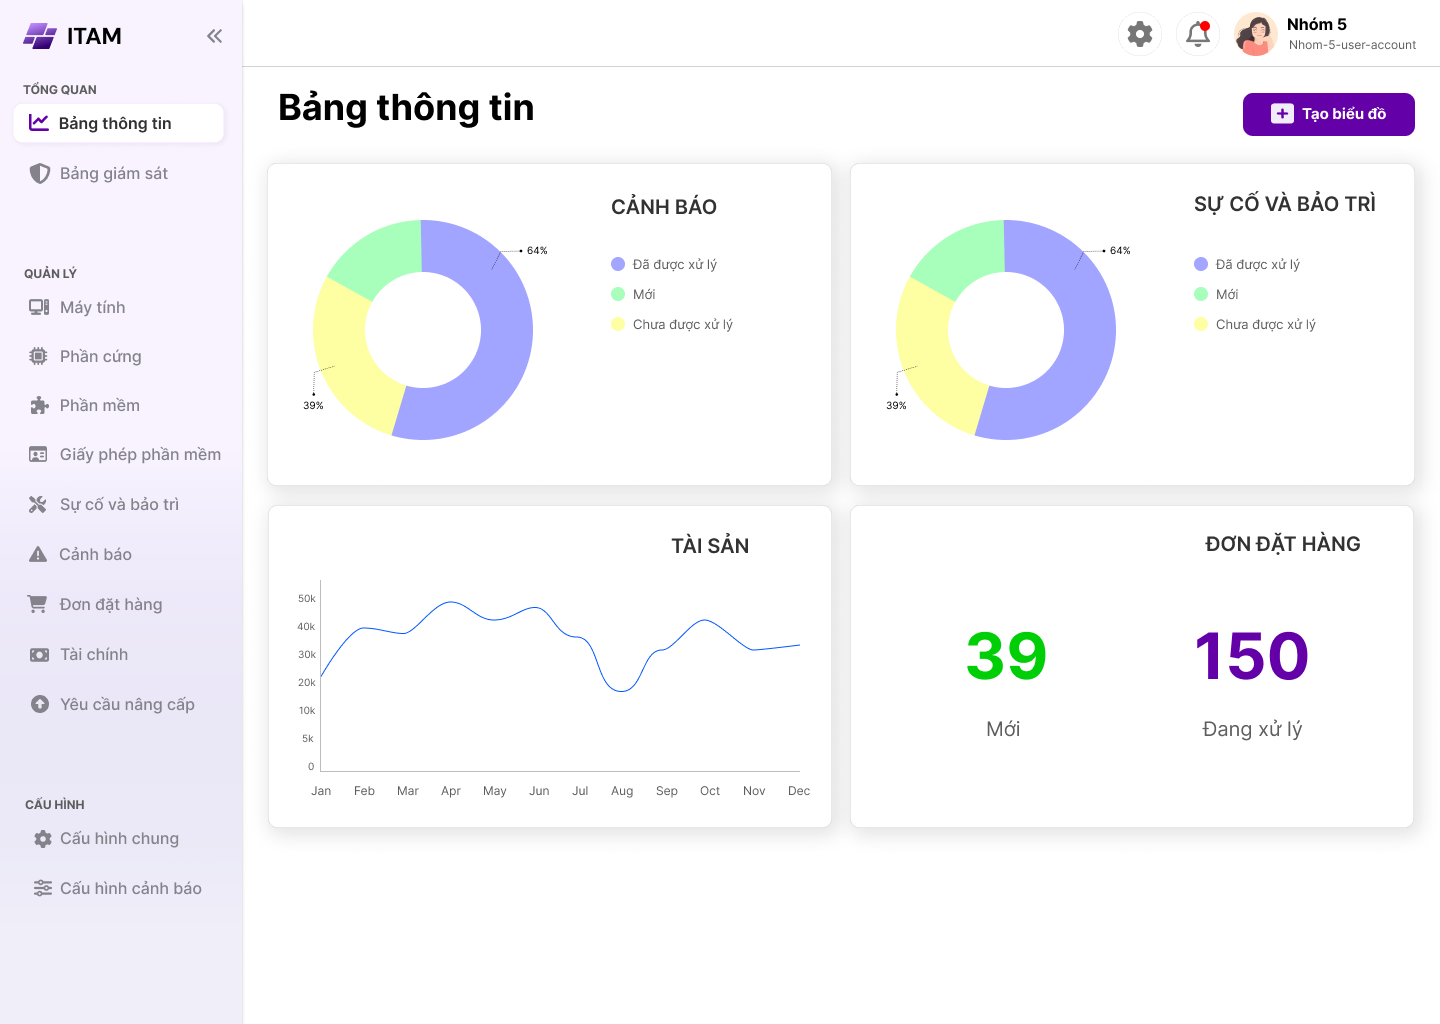
\includegraphics[width=14cm]{Images/C5/UI/Feature-Bảng thông tin.png}
        \vspace{15pt}
        \caption{Giao diện Bảng thông tin}
    \end{figure}

    \item{Bảng giám sát}\\
    \begin{figure}[H]
        \centering
        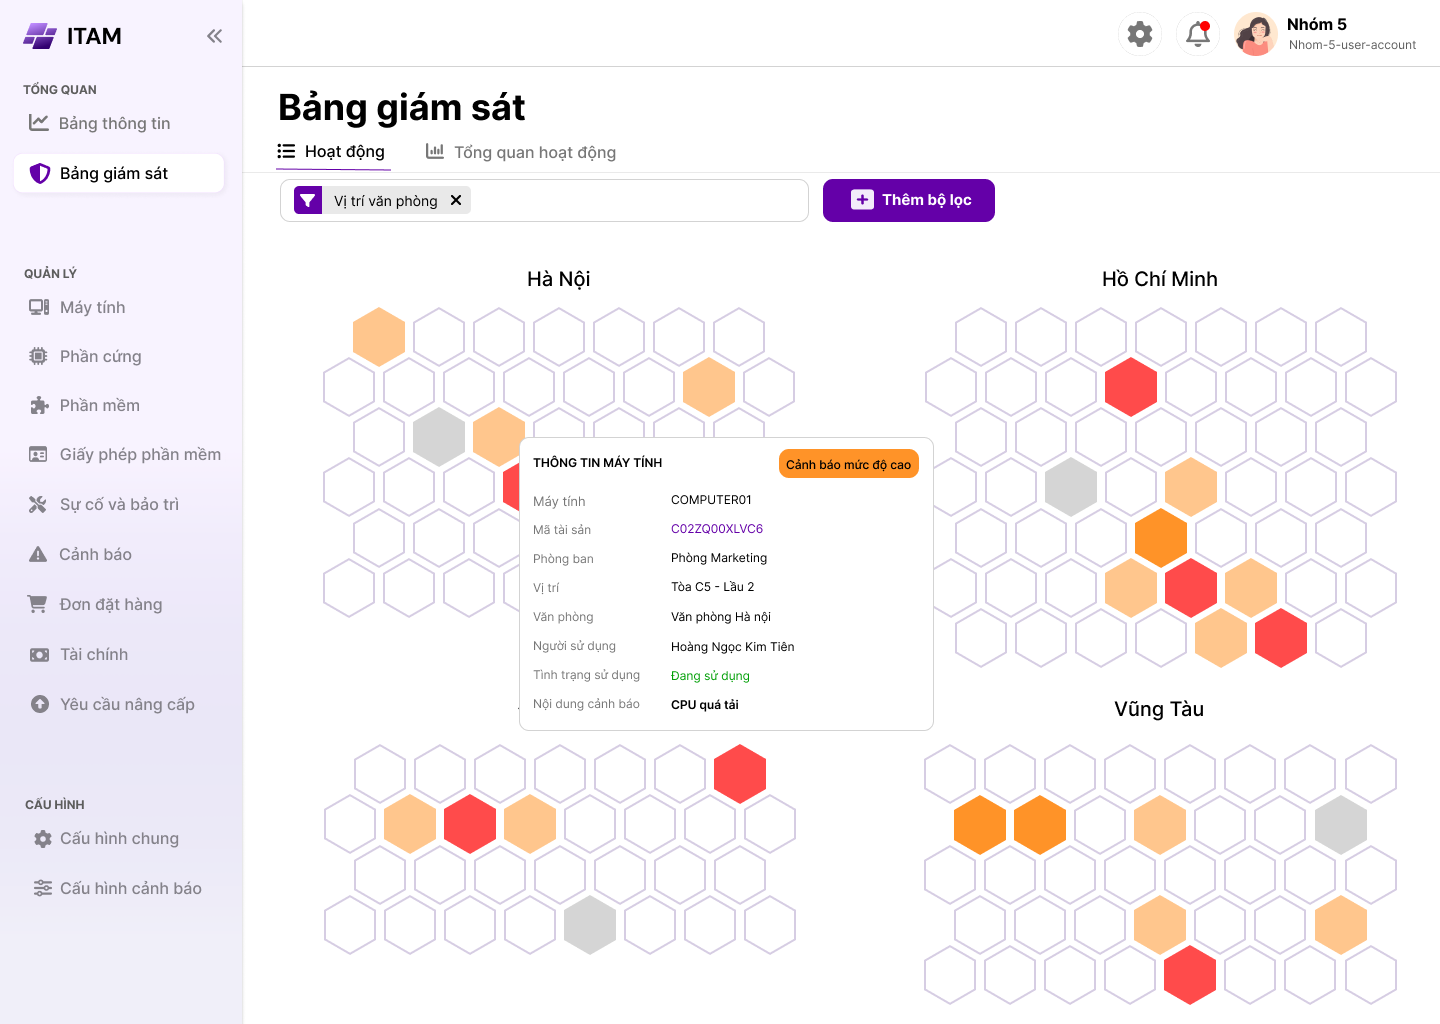
\includegraphics[width=14cm]{Images/C5/UI/Feature-Bảng giám sát 1.3.png}
        \vspace{15pt}
        \caption{Giao diện Bảng giám sát}
    \end{figure}
    \begin{figure}[H]
        \centering
        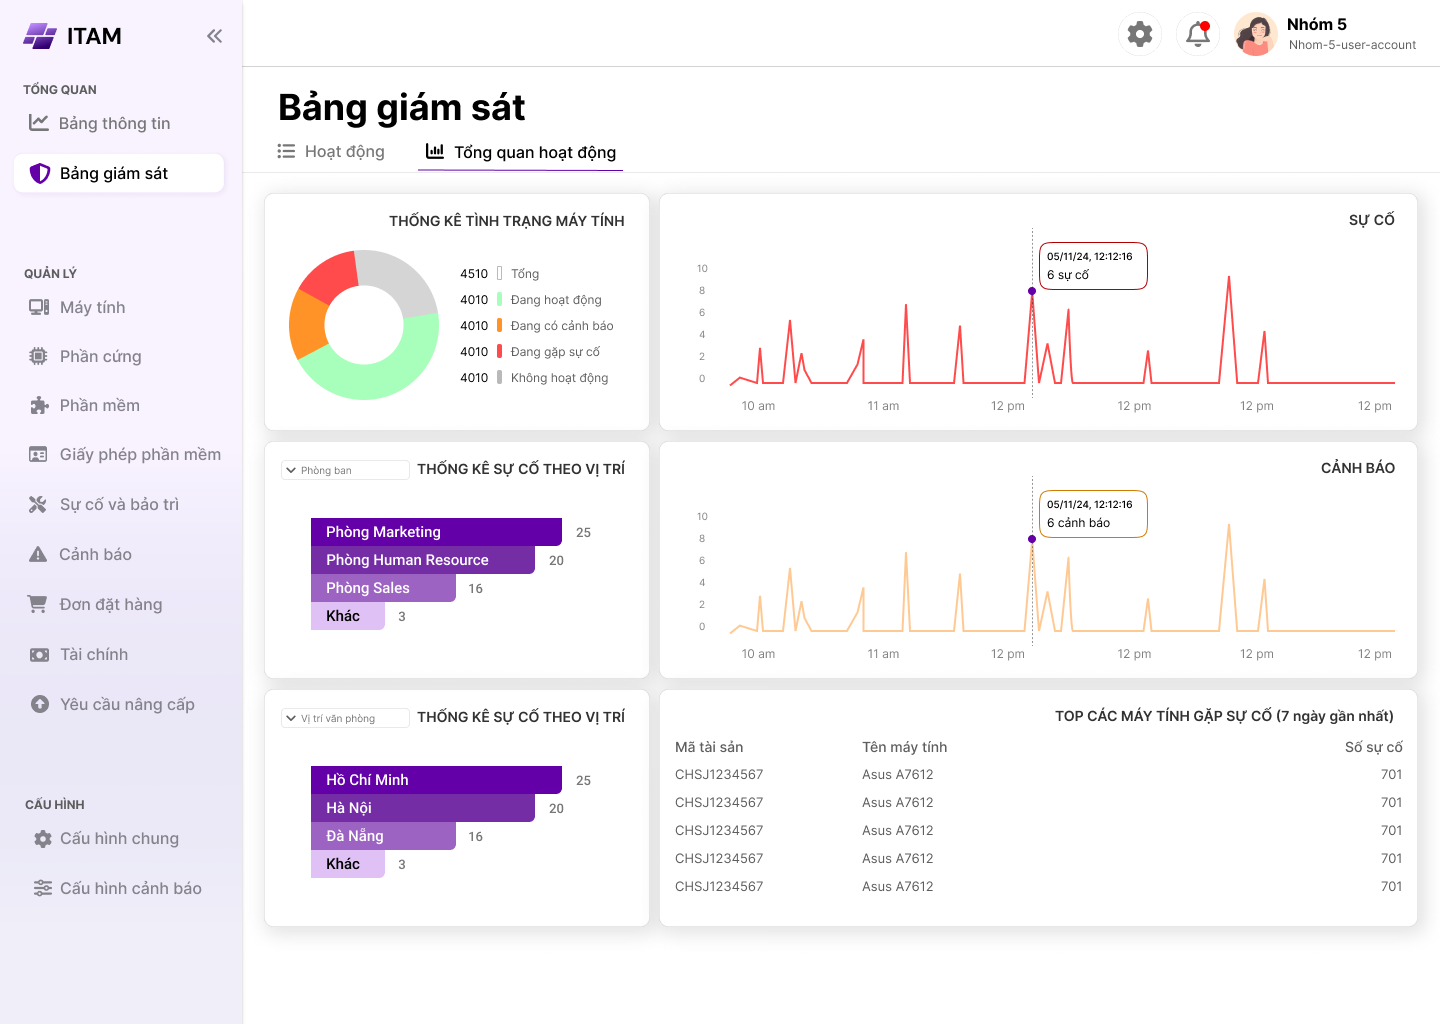
\includegraphics[width=14cm]{Images/C5/UI/Feature-Bảng giám sát 2.png}
        \vspace{15pt}
        \caption{Giao diện Tổng quan giám sát}
    \end{figure}

    \item{Quản lý máy tính}\\
    \begin{figure}[H]
        \centering
        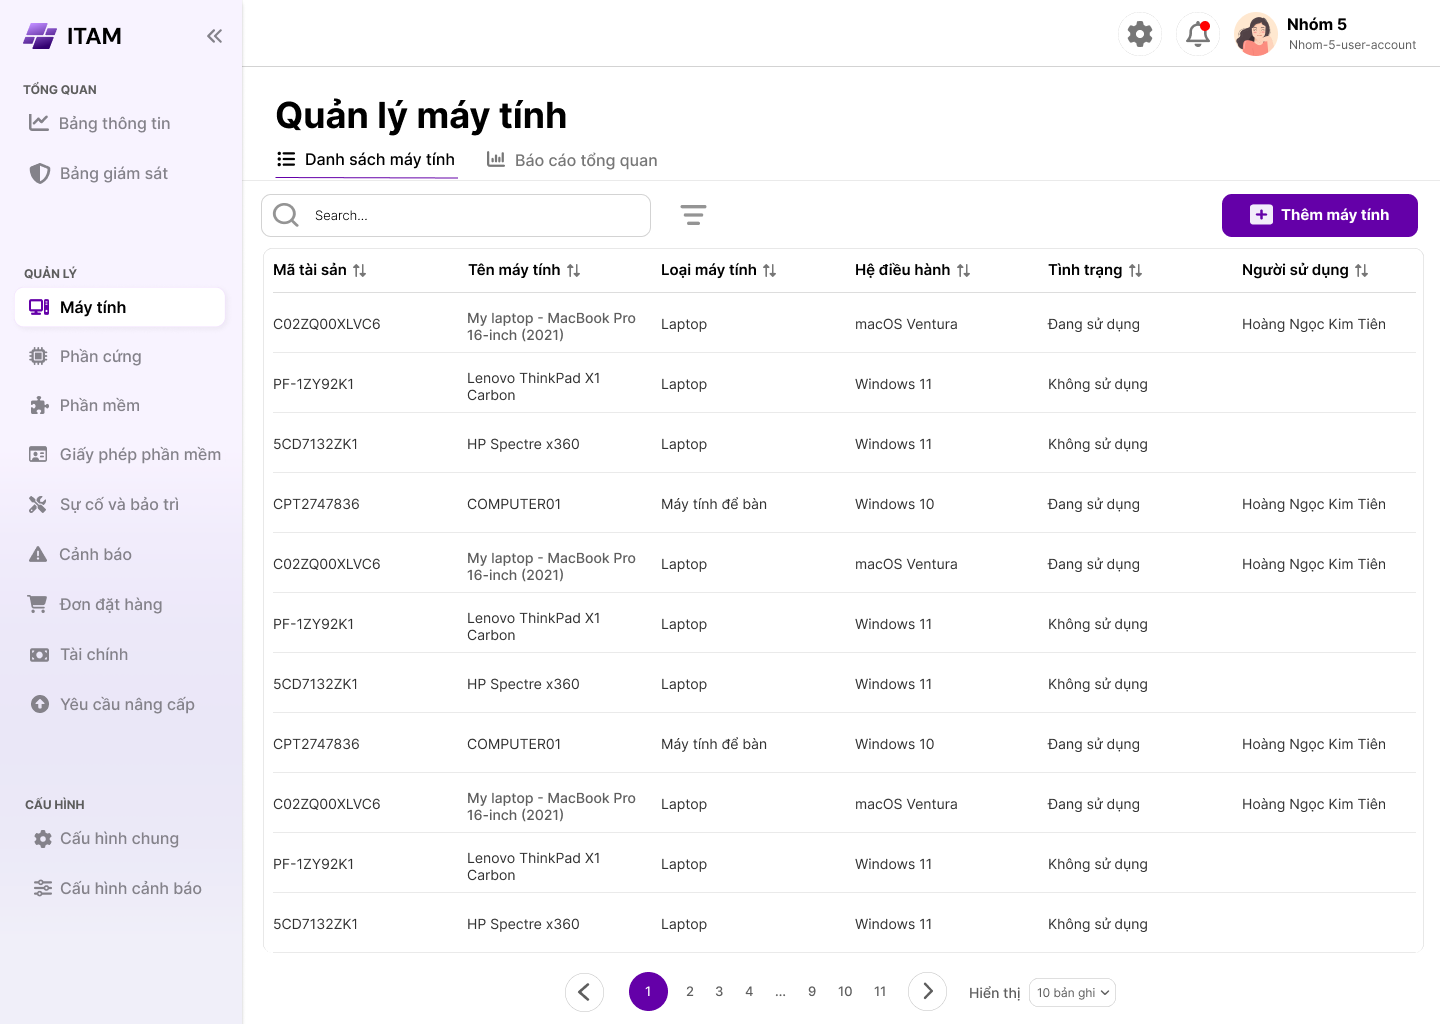
\includegraphics[width=14cm]{Images/C5/UI/Feature-Giám sát tài sản-Máy tính 1.1.png}
        \vspace{15pt}
        \caption{Giao diện Quản lý máy tính 1}
    \end{figure}
    \begin{figure}[H]
        \centering
        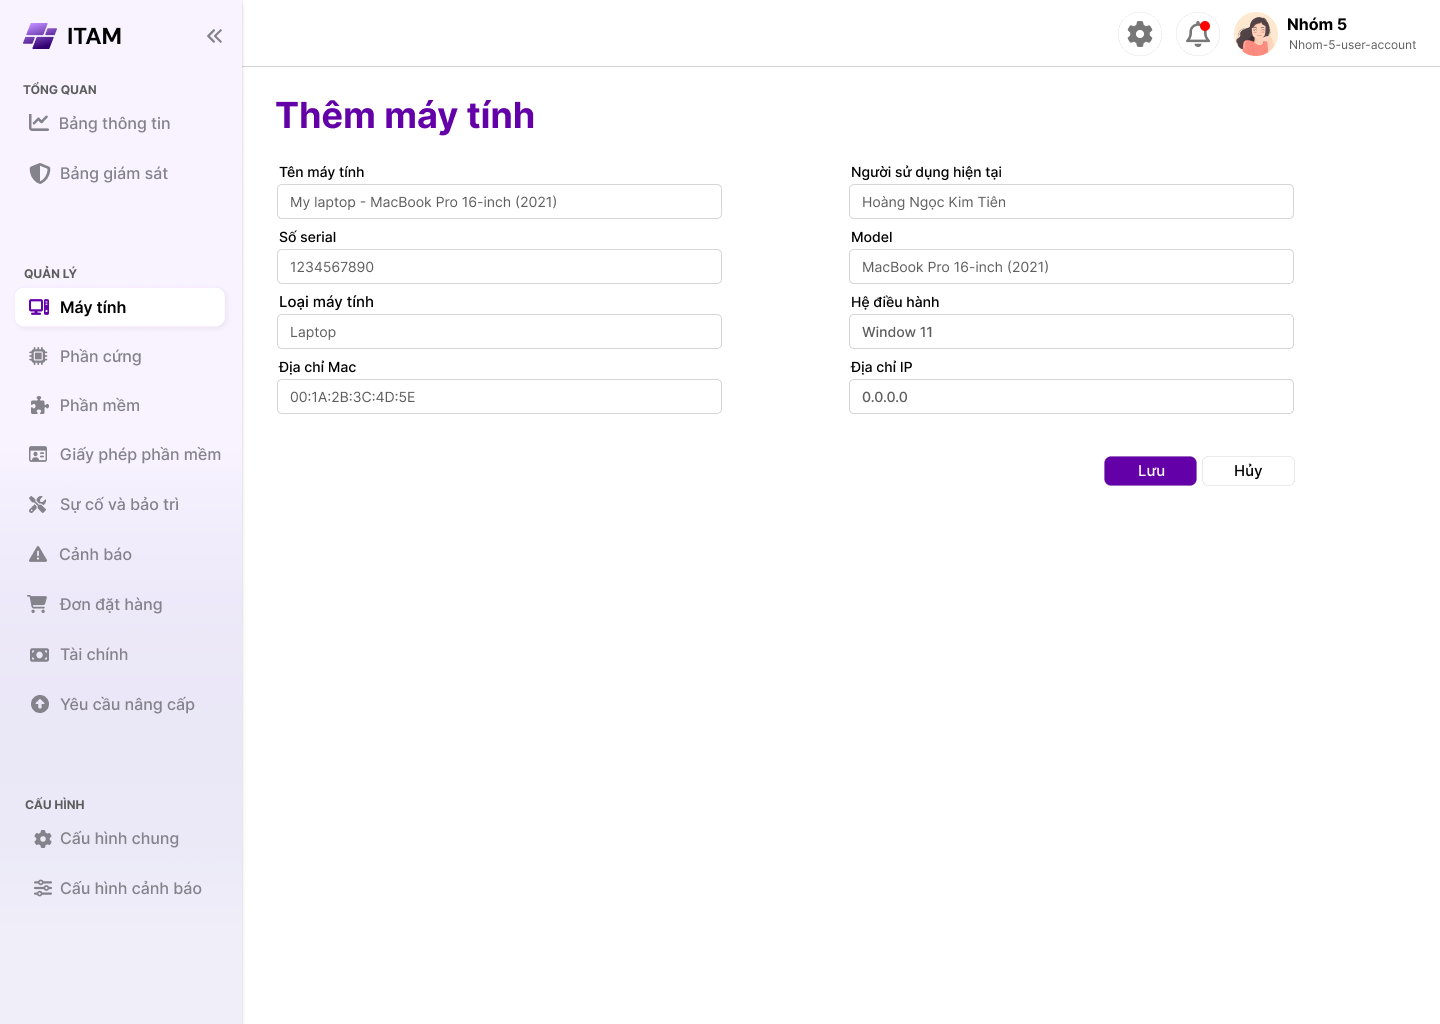
\includegraphics[width=14cm]{Images/C5/UI/Feature-Giám sát tài sản-Máy tính 1.2.png}
        \vspace{15pt}
        \caption{Giao diện Quản lý máy tính 2}
    \end{figure}
    % \begin{figure}[H]
    %     \centering
    %     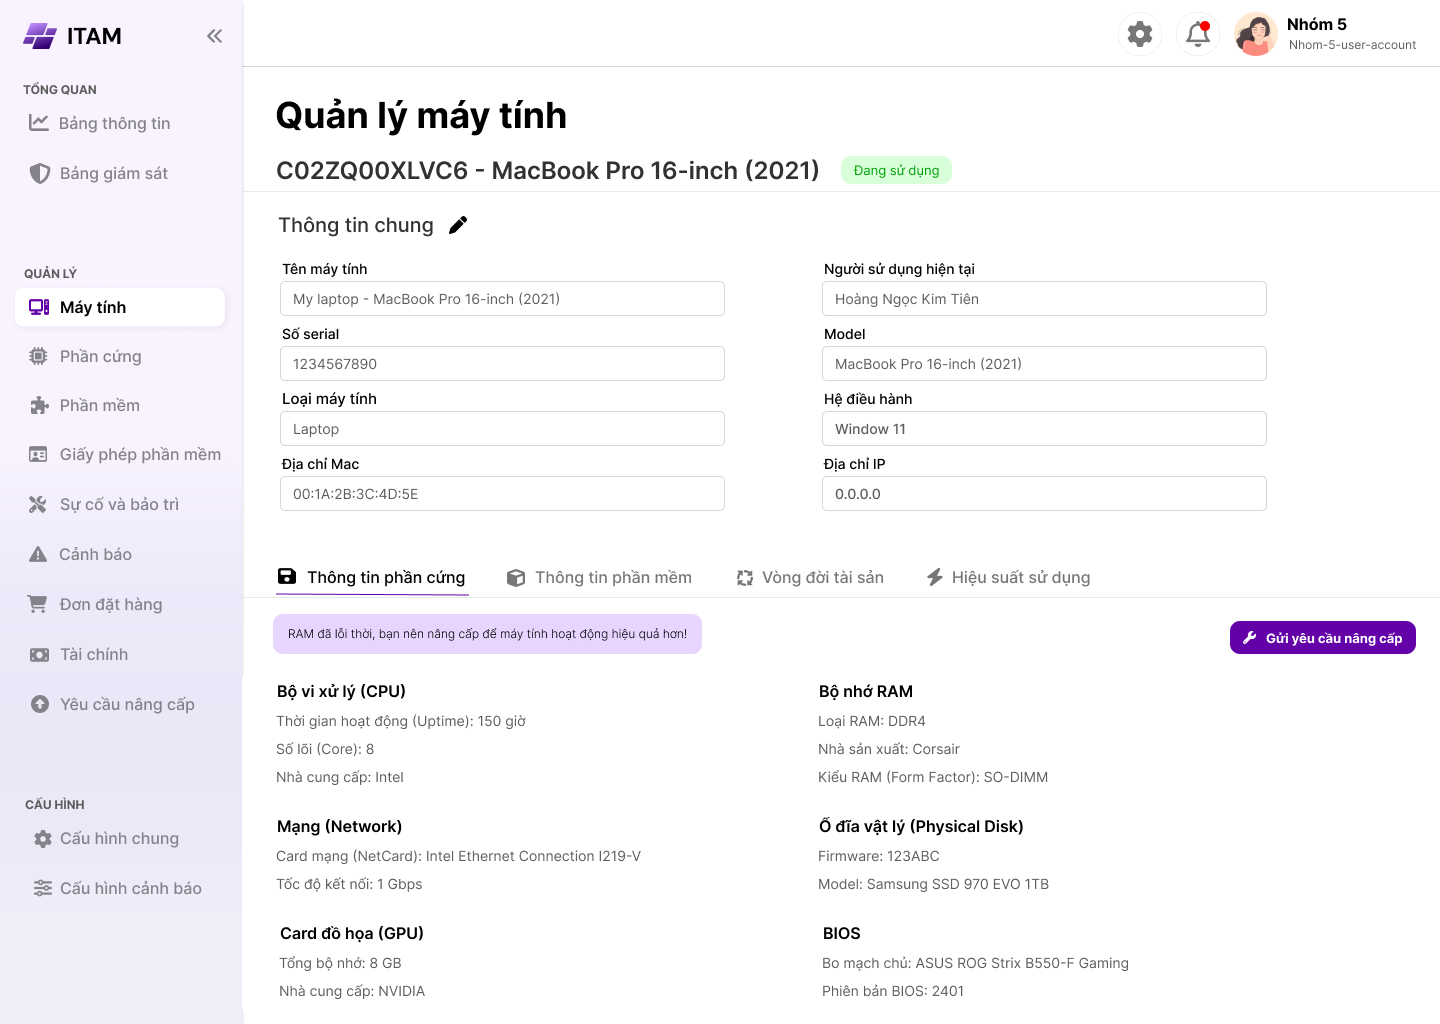
\includegraphics[width=14cm]{Images/C5/UI/Feature-Giám sát tài sản-Máy tính 2.1.png}
    %     \vspace{15pt}
    %     \caption{Giao diện Quản lý máy tính 3}
    % \end{figure}
    \begin{figure}[H]
        \centering
        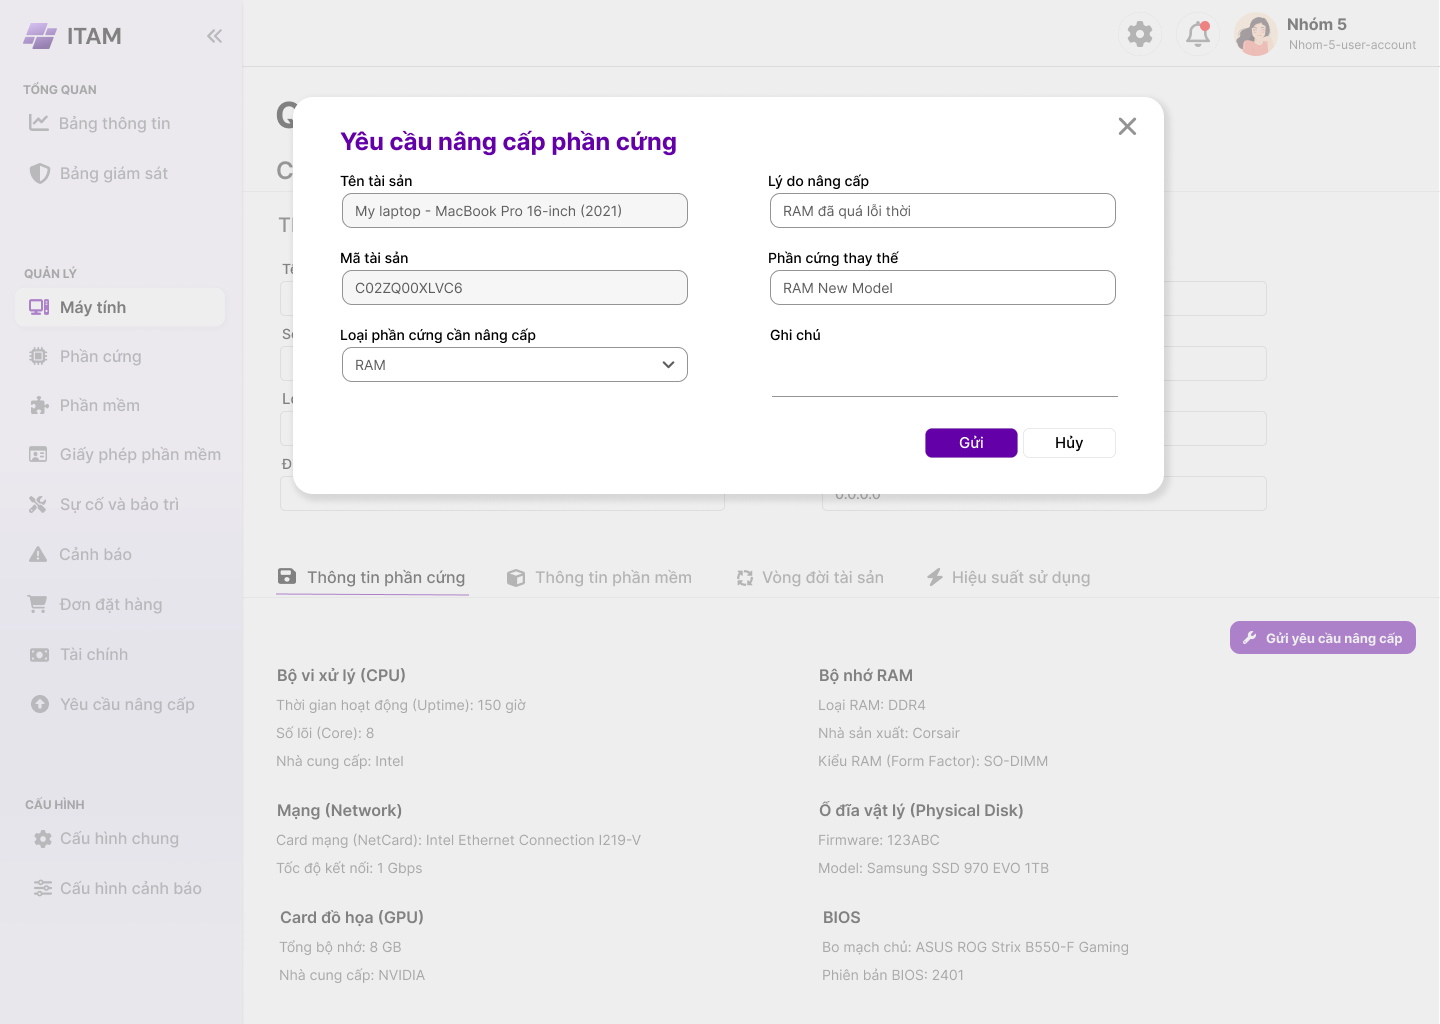
\includegraphics[width=14cm]{Images/C5/UI/Feature-Giám sát tài sản-Máy tính 2.2.png}
        \vspace{15pt}
        \caption{Giao diện Quản lý máy tính 3}
    \end{figure}
    \begin{figure}[H]
        \centering
        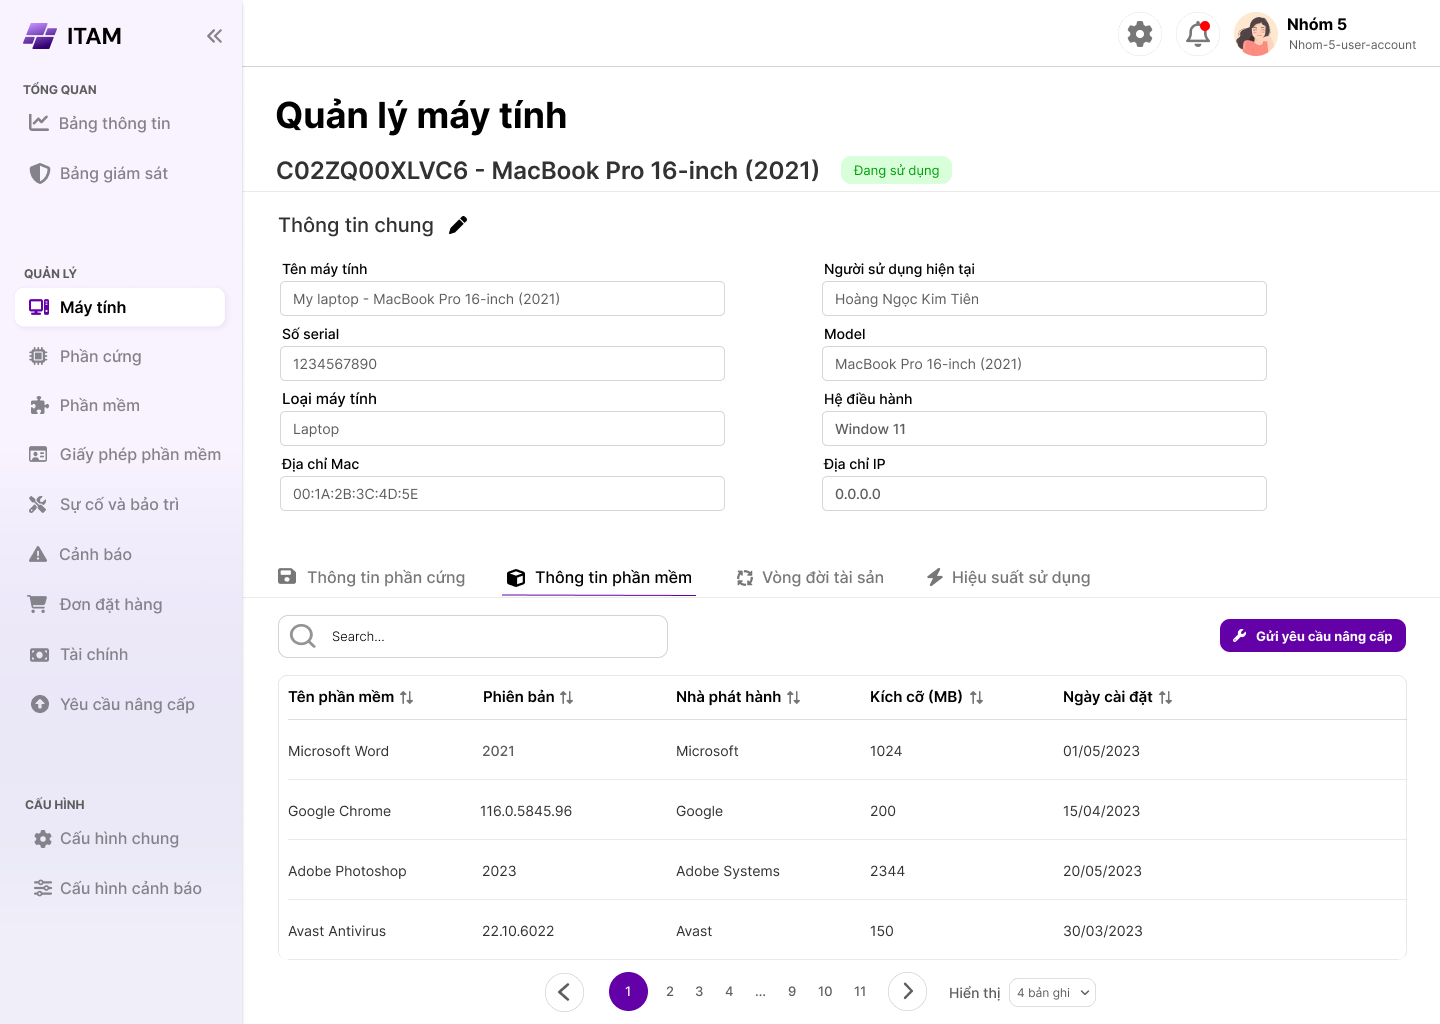
\includegraphics[width=14cm]{Images/C5/UI/Feature-Giám sát tài sản-Máy tính 3.1.png}
        \vspace{15pt}
        \caption{Giao diện Quản lý máy tính 4}
    \end{figure}
    \begin{figure}[H]
        \centering
        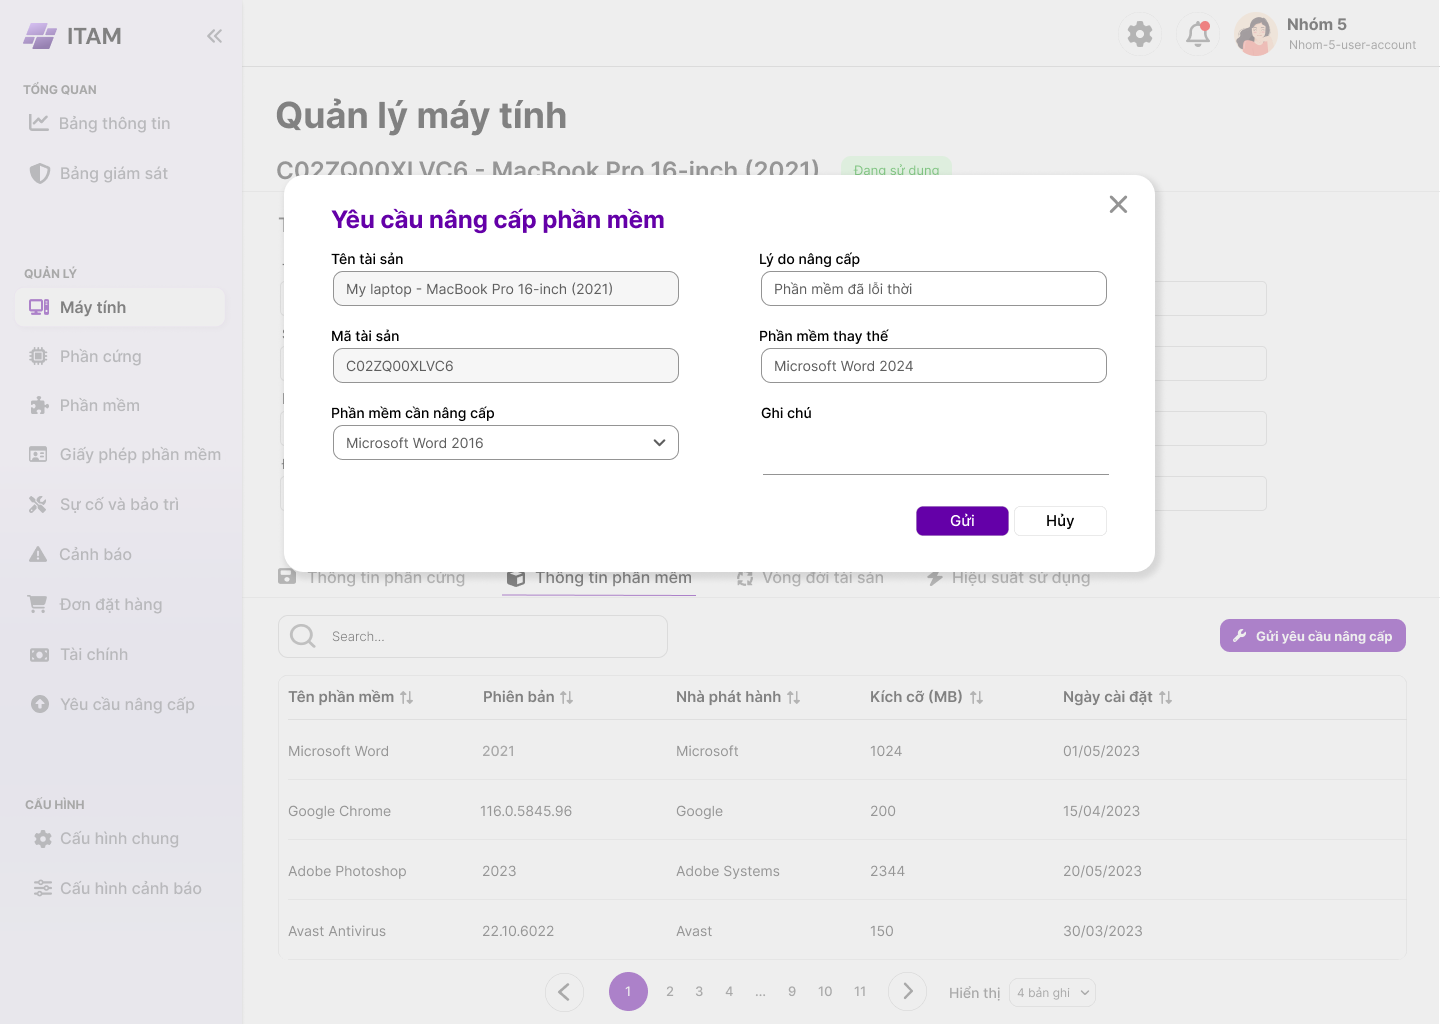
\includegraphics[width=14cm]{Images/C5/UI/Feature-Giám sát tài sản-Máy tính 3.2.png}
        \vspace{15pt}
        \caption{Giao diện Quản lý máy tính 5}
    \end{figure}
    \begin{figure}[H]
        \centering
        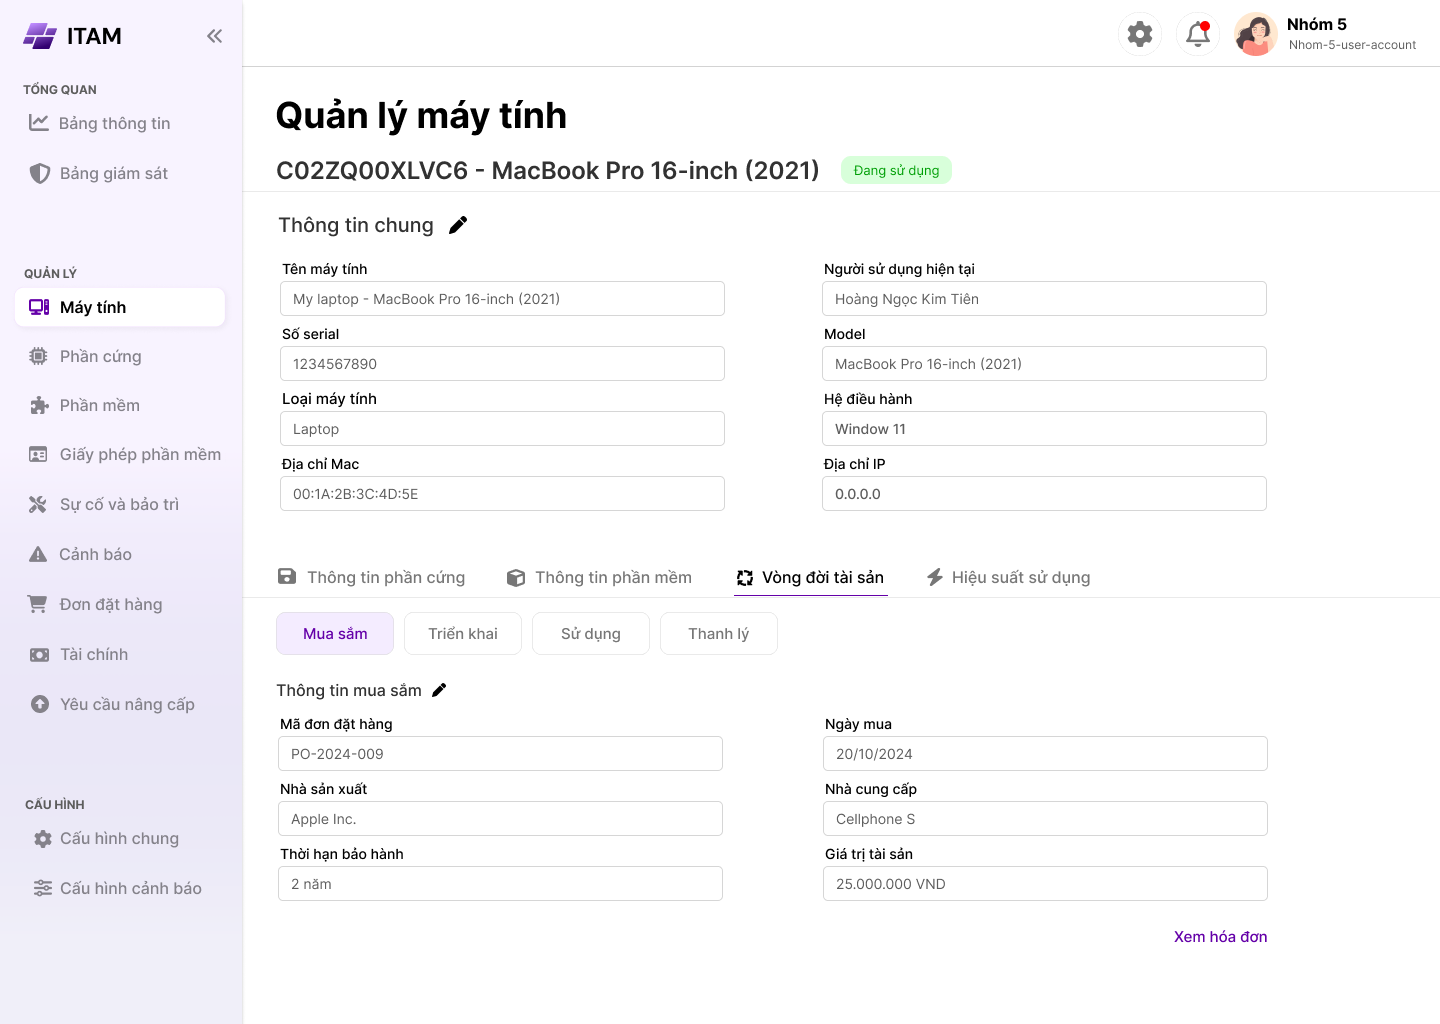
\includegraphics[width=14cm]{Images/C5/UI/Feature-Giám sát tài sản-Máy tính 4.1.png}
        \vspace{15pt}
        \caption{Giao diện Quản lý máy tính 6}
    \end{figure}
    \begin{figure}[H]
    \centering
    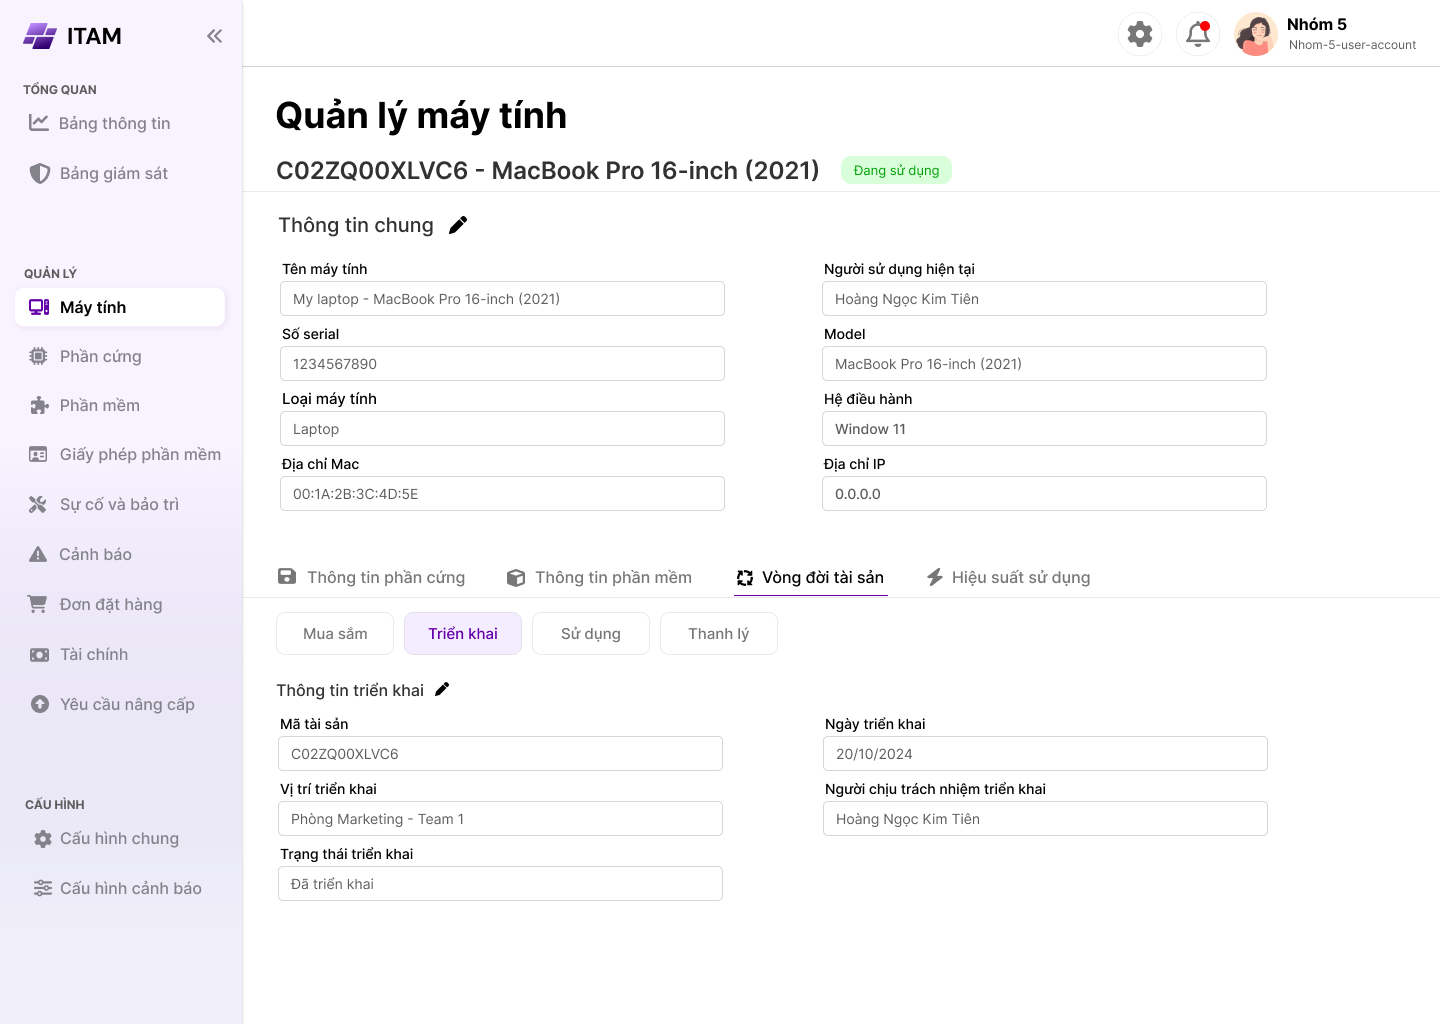
\includegraphics[width=14cm]{Images/C5/UI/Feature-Giám sát tài sản-Máy tính 5.png}
    \vspace{15pt}
    \caption{Giao diện Quản lý máy tính 7}
    \end{figure}
    \begin{figure}[H]
        \centering
        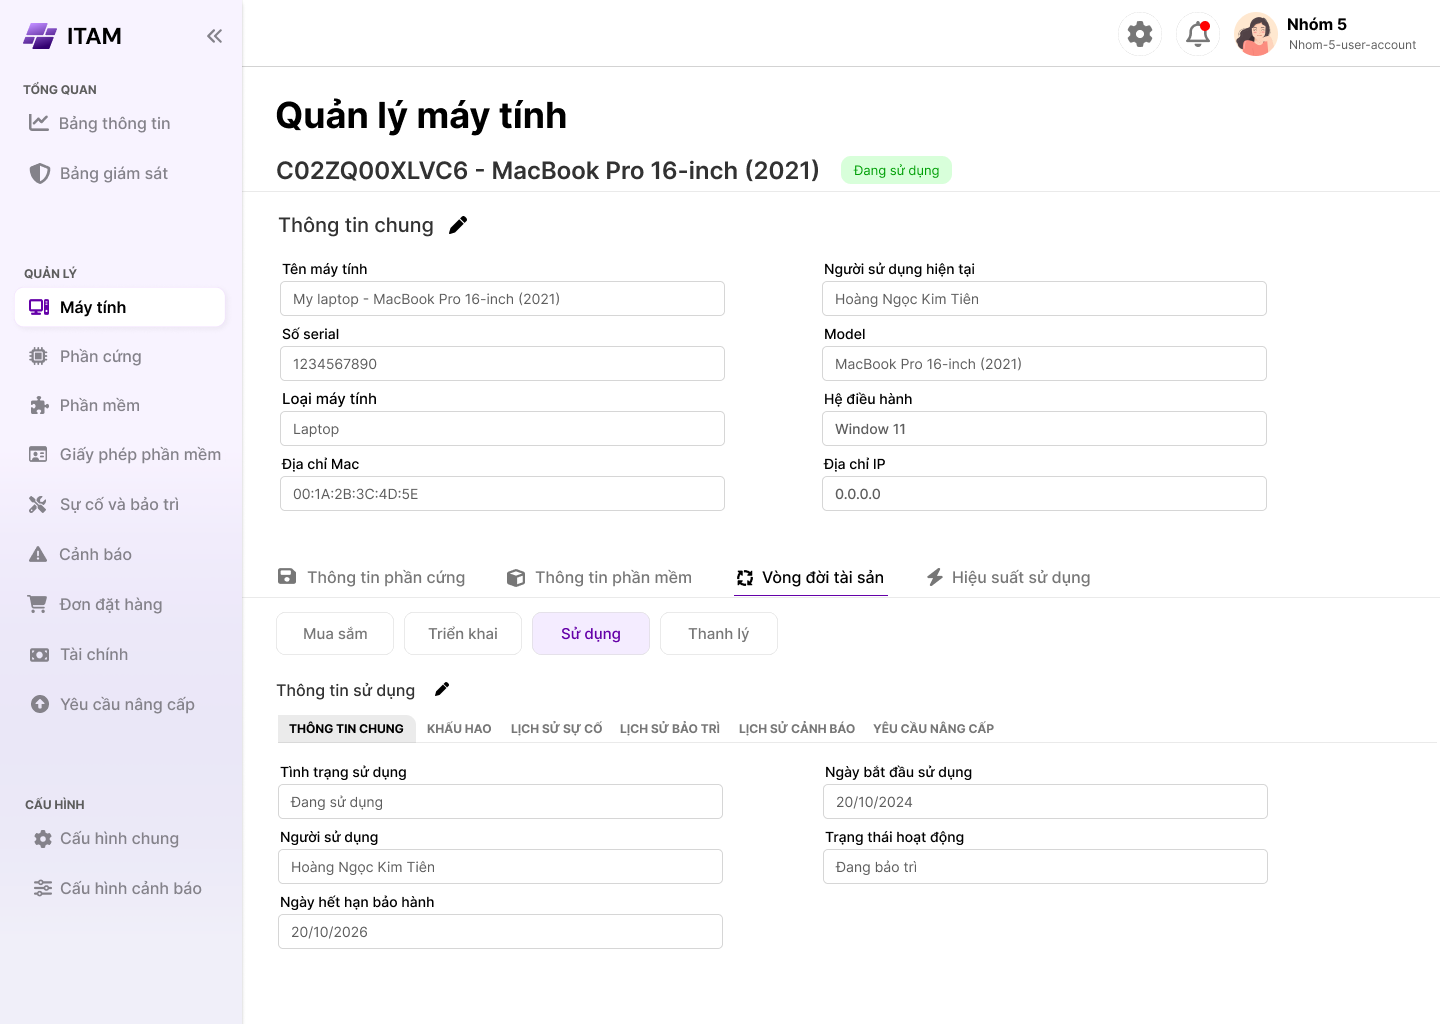
\includegraphics[width=14cm]{Images/C5/UI/Feature-Giám sát tài sản-Máy tính 6.1.png}
        \vspace{15pt}
        \caption{Giao diện Quản lý máy tính 8}
    \end{figure}
    \begin{figure}[H]
        \centering
        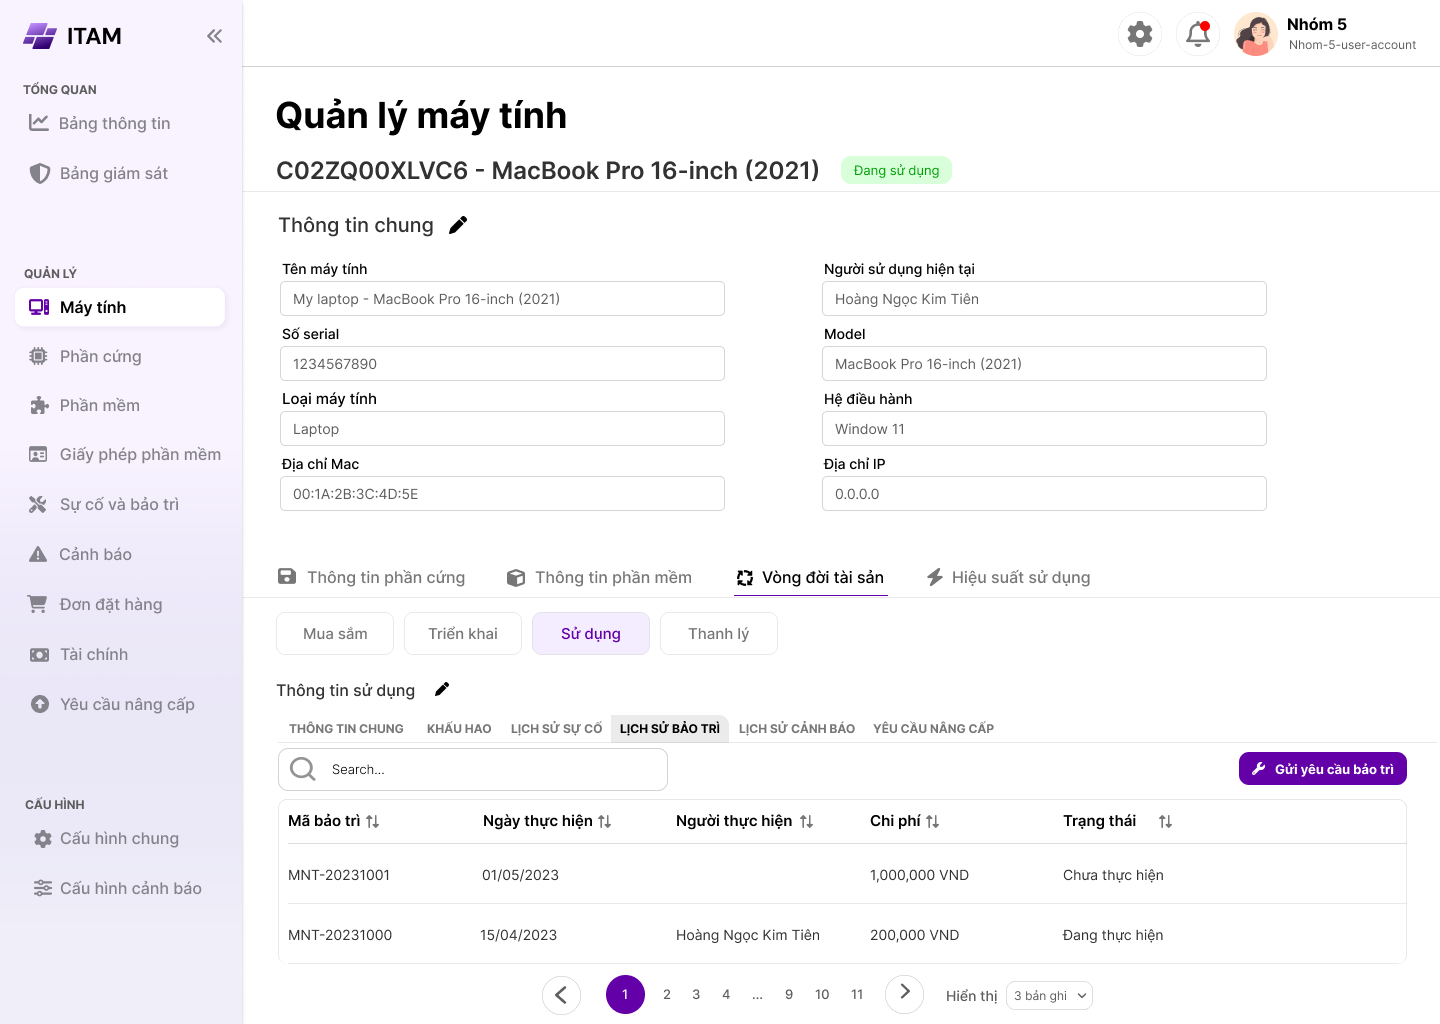
\includegraphics[width=14cm]{Images/C5/UI/Feature-Giám sát tài sản-Máy tính 6.8.png}
        \vspace{15pt}
        \caption{Giao diện Quản lý máy tính 9}
    \end{figure}
    \begin{figure}[H]
        \centering
        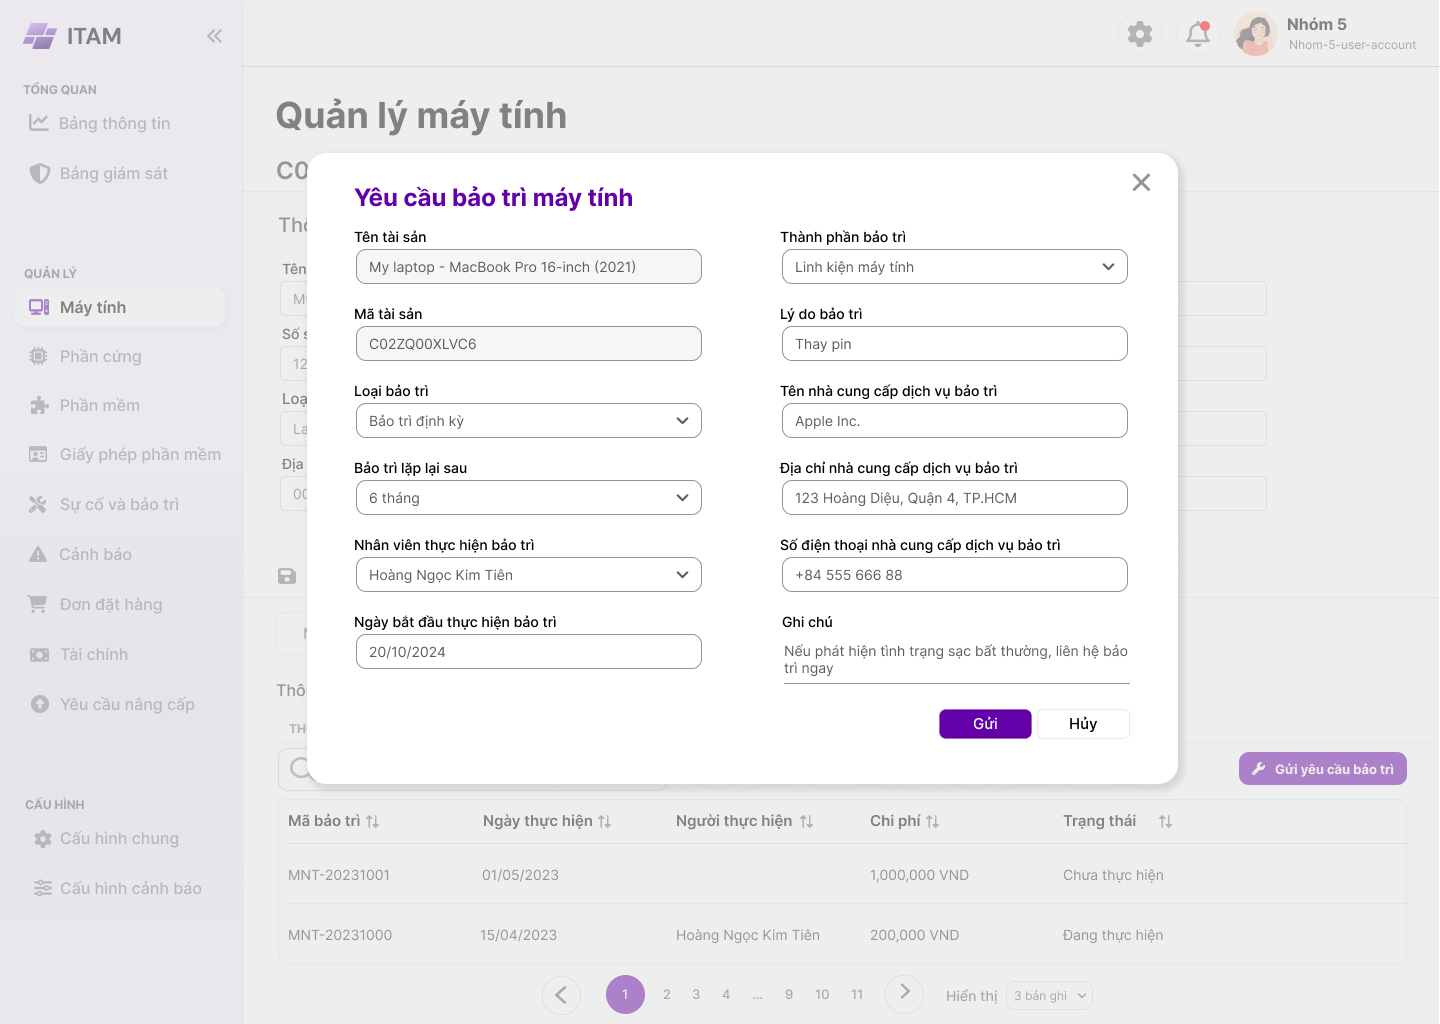
\includegraphics[width=14cm]{Images/C5/UI/Feature-Giám sát tài sản-Máy tính 6.12.png}
        \vspace{15pt}
        \caption{Giao diện Quản lý máy tính 10}
    \end{figure}
    \begin{figure}[H]
        \centering
        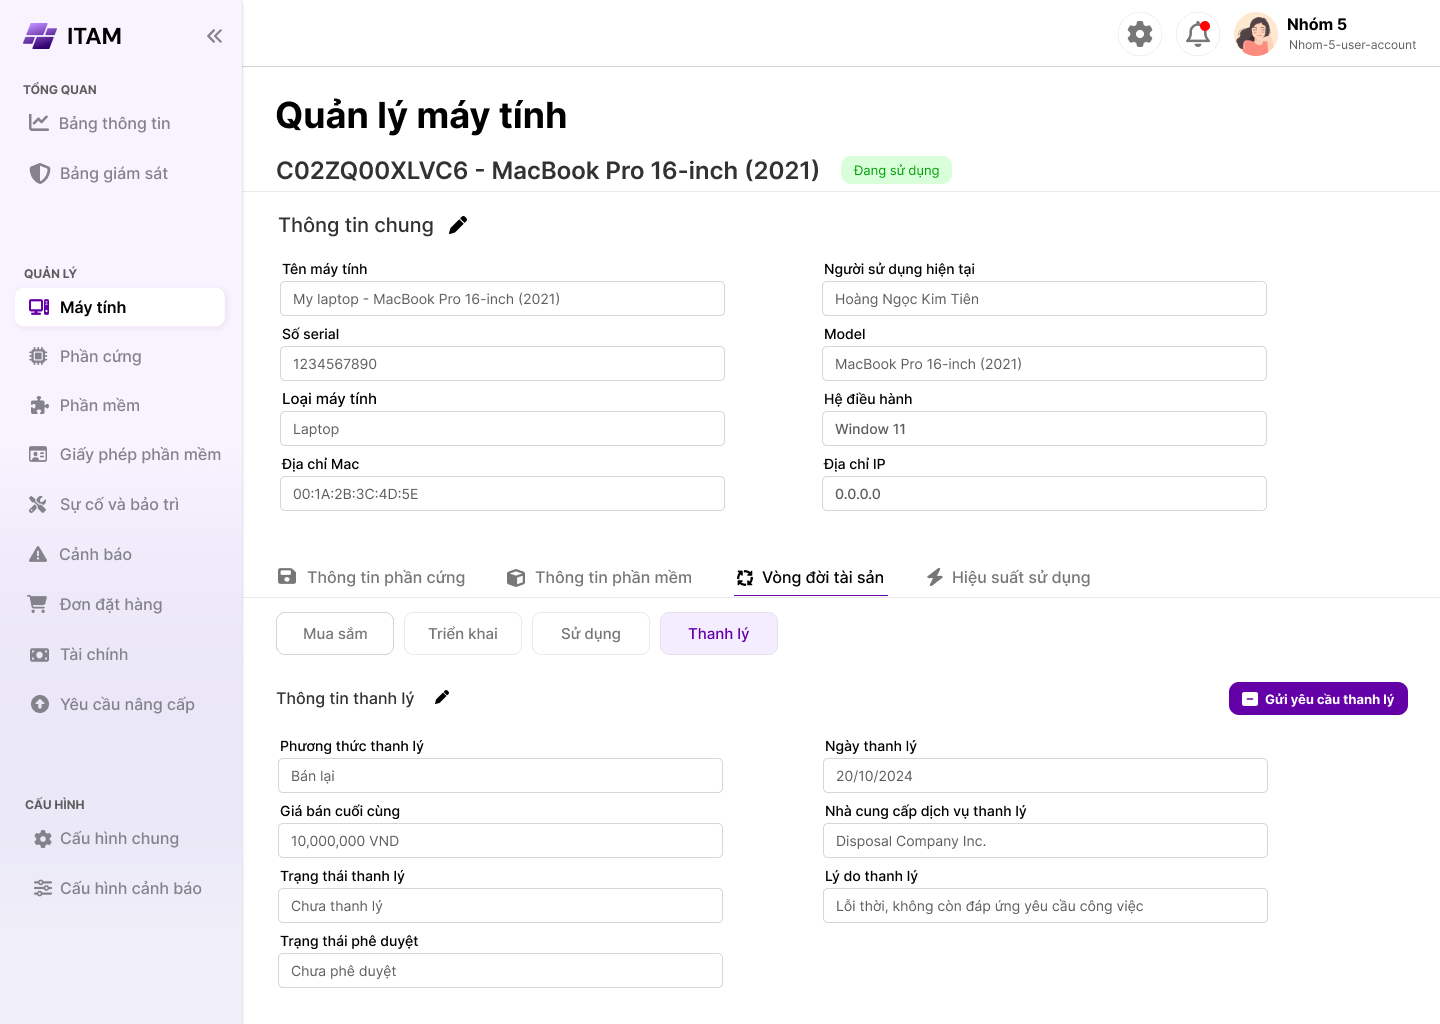
\includegraphics[width=14cm]{Images/C5/UI/Feature-Giám sát tài sản-Máy tính 7.1.png}
        \vspace{15pt}
        \caption{Giao diện Quản lý máy tính 11}
    \end{figure}
    \begin{figure}[H]
        \centering
        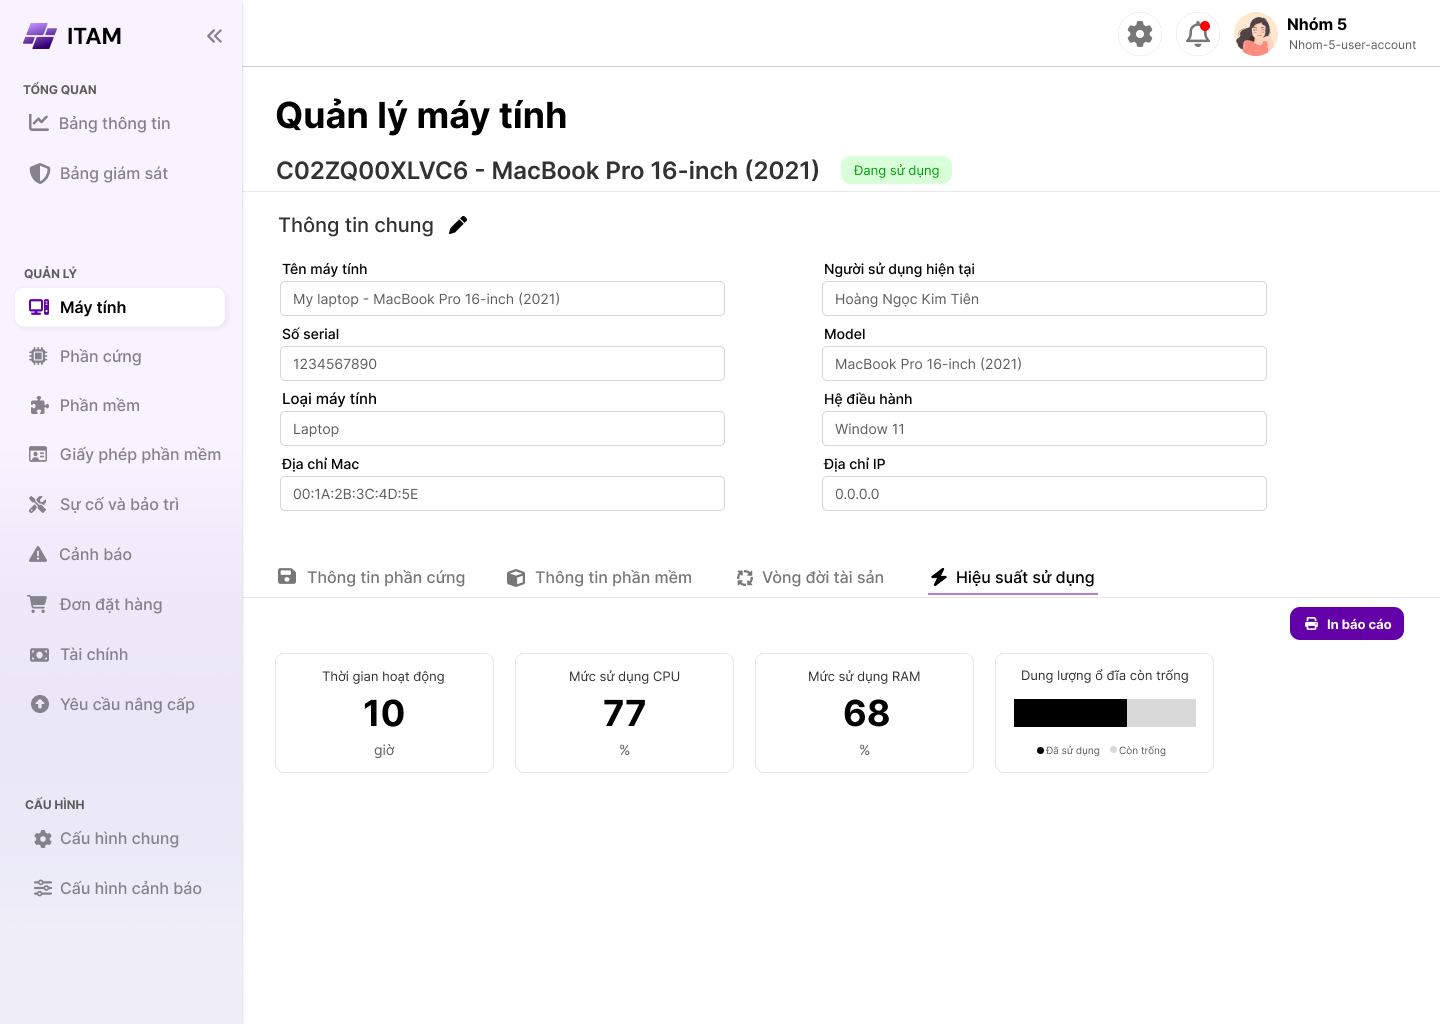
\includegraphics[width=14cm]{Images/C5/UI/Feature-Giám sát tài sản-Máy tính 9.1.png}
        \vspace{15pt}
        \caption{Giao diện Quản lý máy tính 12}
    \end{figure}
    % \begin{figure}[H]
    %     \centering
    %     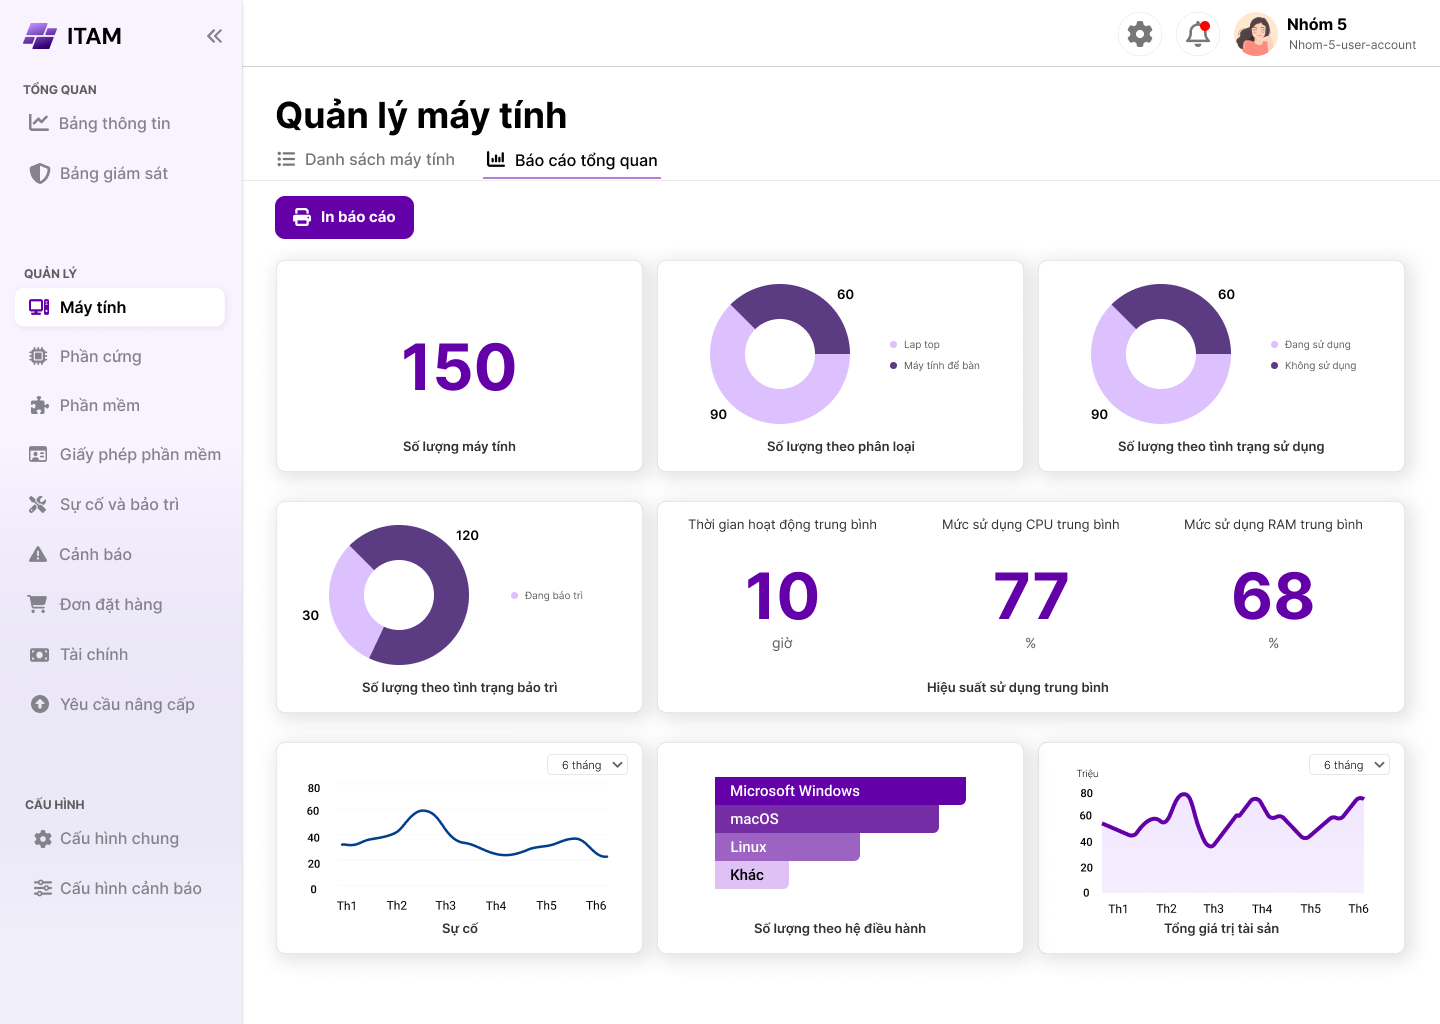
\includegraphics[width=14cm]{Images/C5/UI/Feature-Giám sát tài sản-Máy tính 10.png}
    %     \vspace{15pt}
    %     \caption{Giao diện Quản lý máy tính 14}
    % \end{figure}

    \item{Quản lý phần cứng}\\
    \begin{figure}[H]
        \centering
        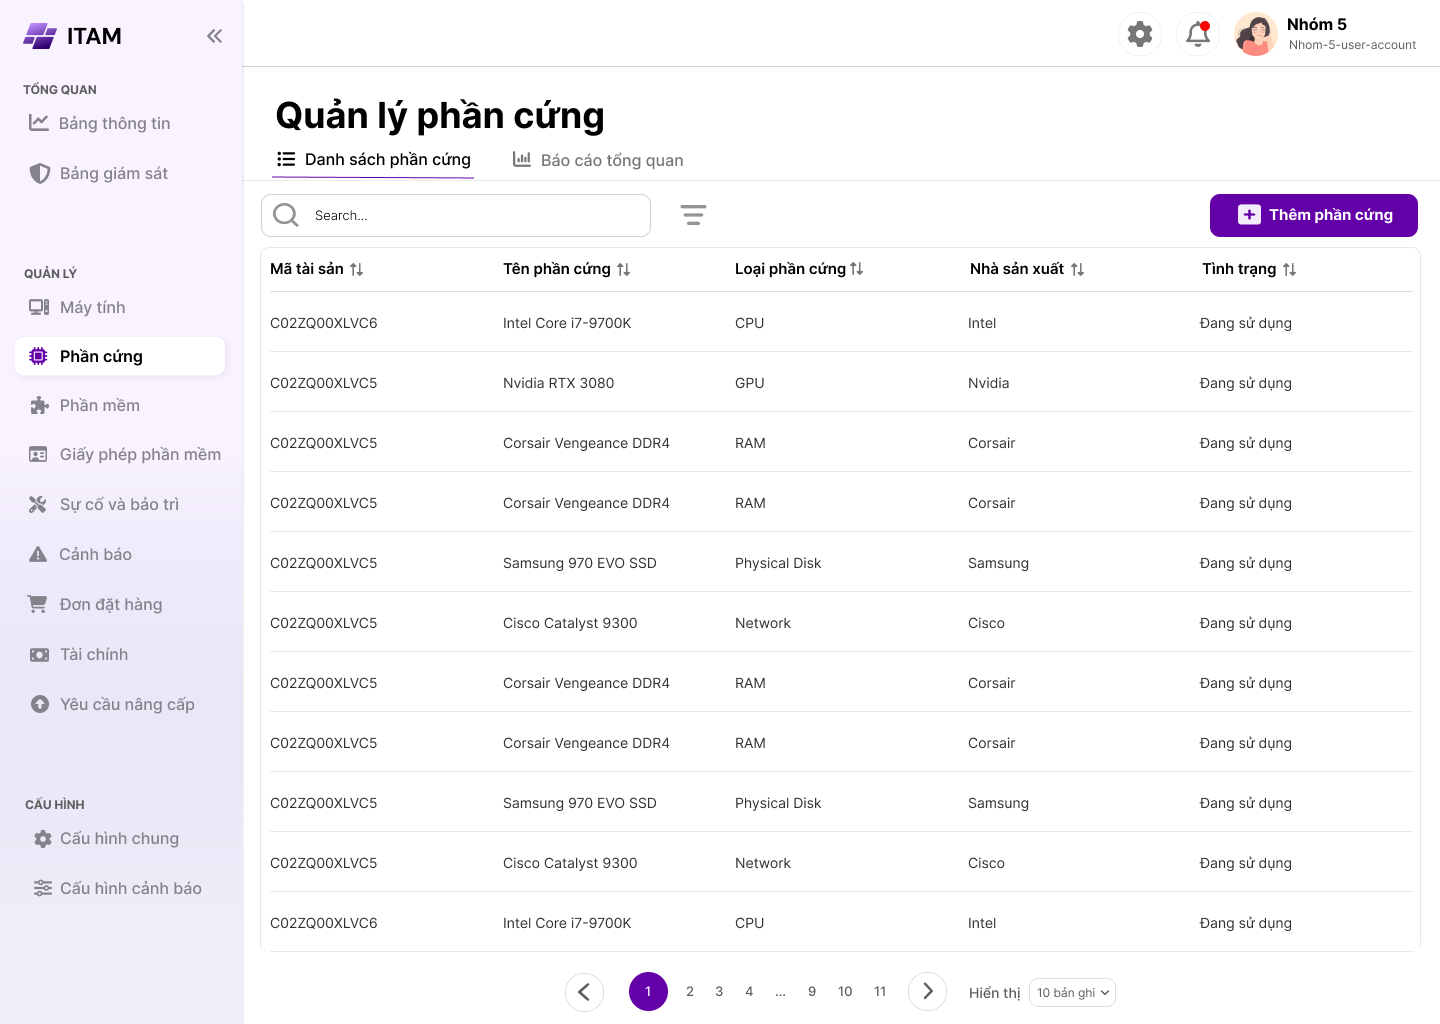
\includegraphics[width=14cm]{Images/C5/UI/Feature-Giám sát tài sản-Phần cứng 1.png}
        \vspace{15pt}
        \caption{Giao diện Quản lý phần cứng 1}
    \end{figure}
    \begin{figure}[H]
        \centering
        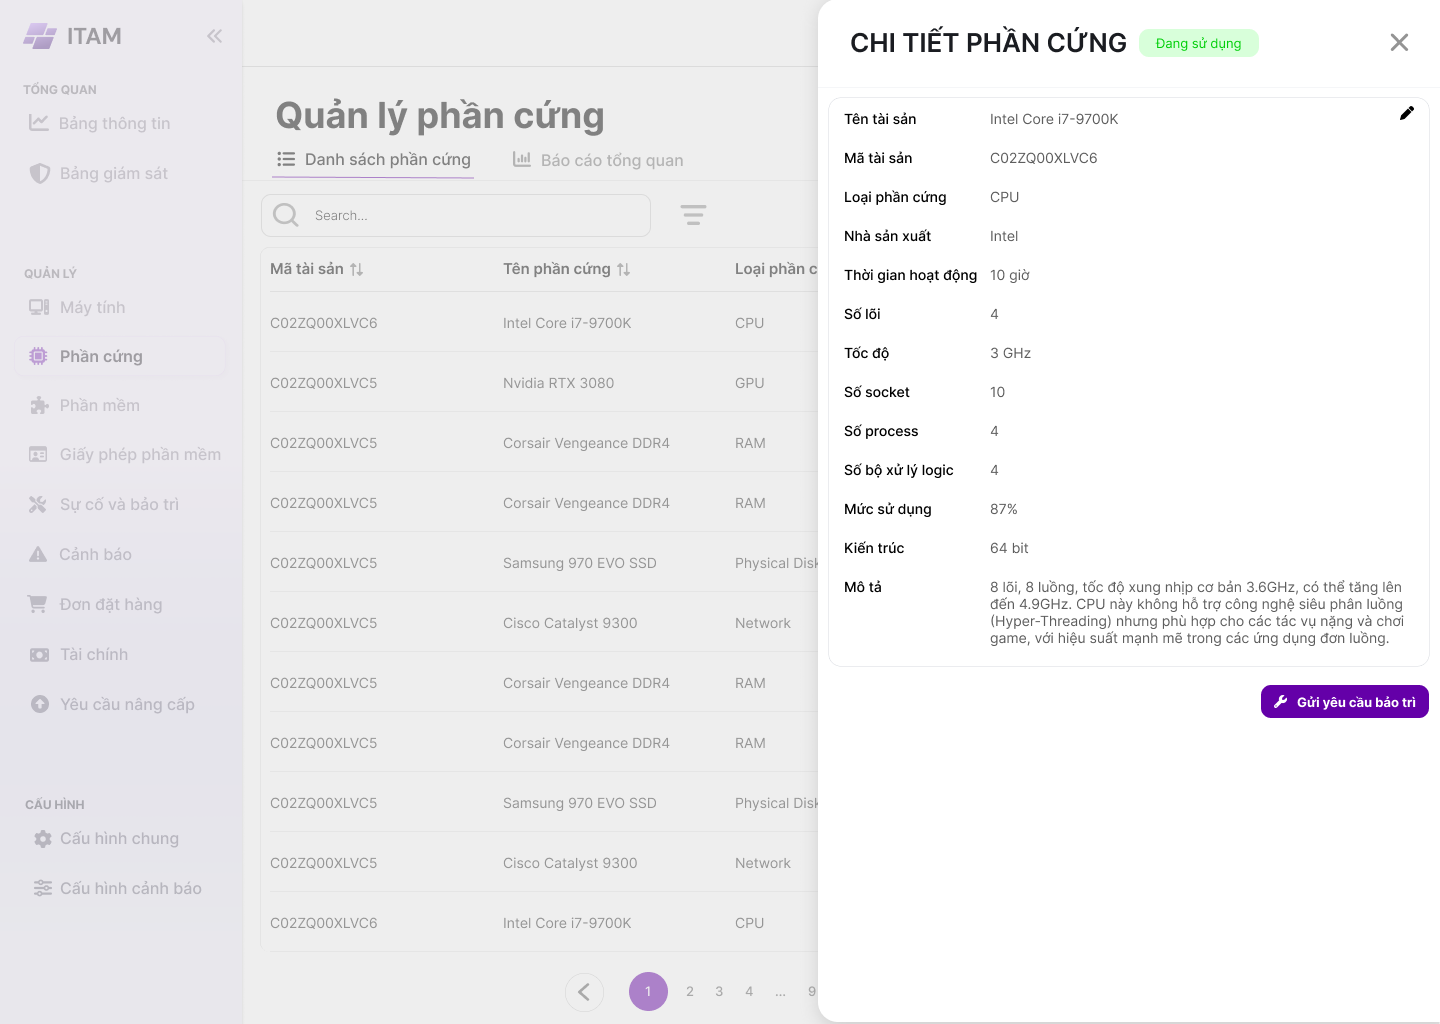
\includegraphics[width=14cm]{Images/C5/UI/Feature-Giám sát tài sản-Phần cứng 2.1-CPU.png}
        \vspace{15pt}
        \caption{Giao diện Quản lý phần cứng 2}
    \end{figure}
    \begin{figure}[H]
        \centering
        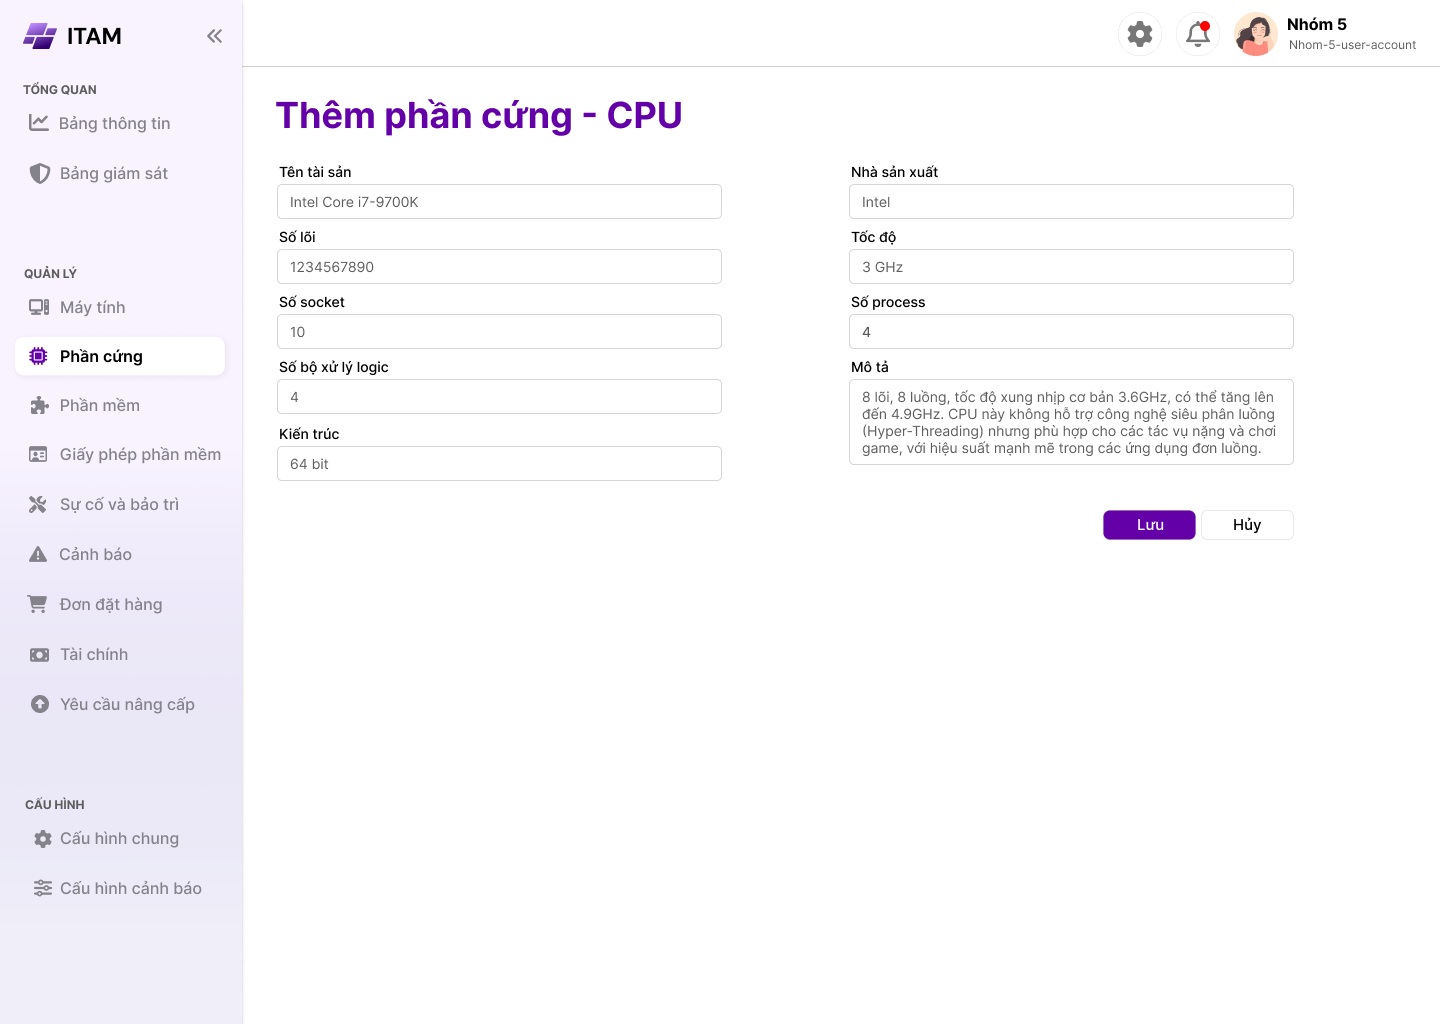
\includegraphics[width=14cm]{Images/C5/UI/Feature-Giám sát tài sản-Phần cứng 4.2.png}
        \vspace{15pt}
        \caption{Giao diện Quản lý phần cứng 3}
    \end{figure}
    \begin{figure}[H]
        \centering
        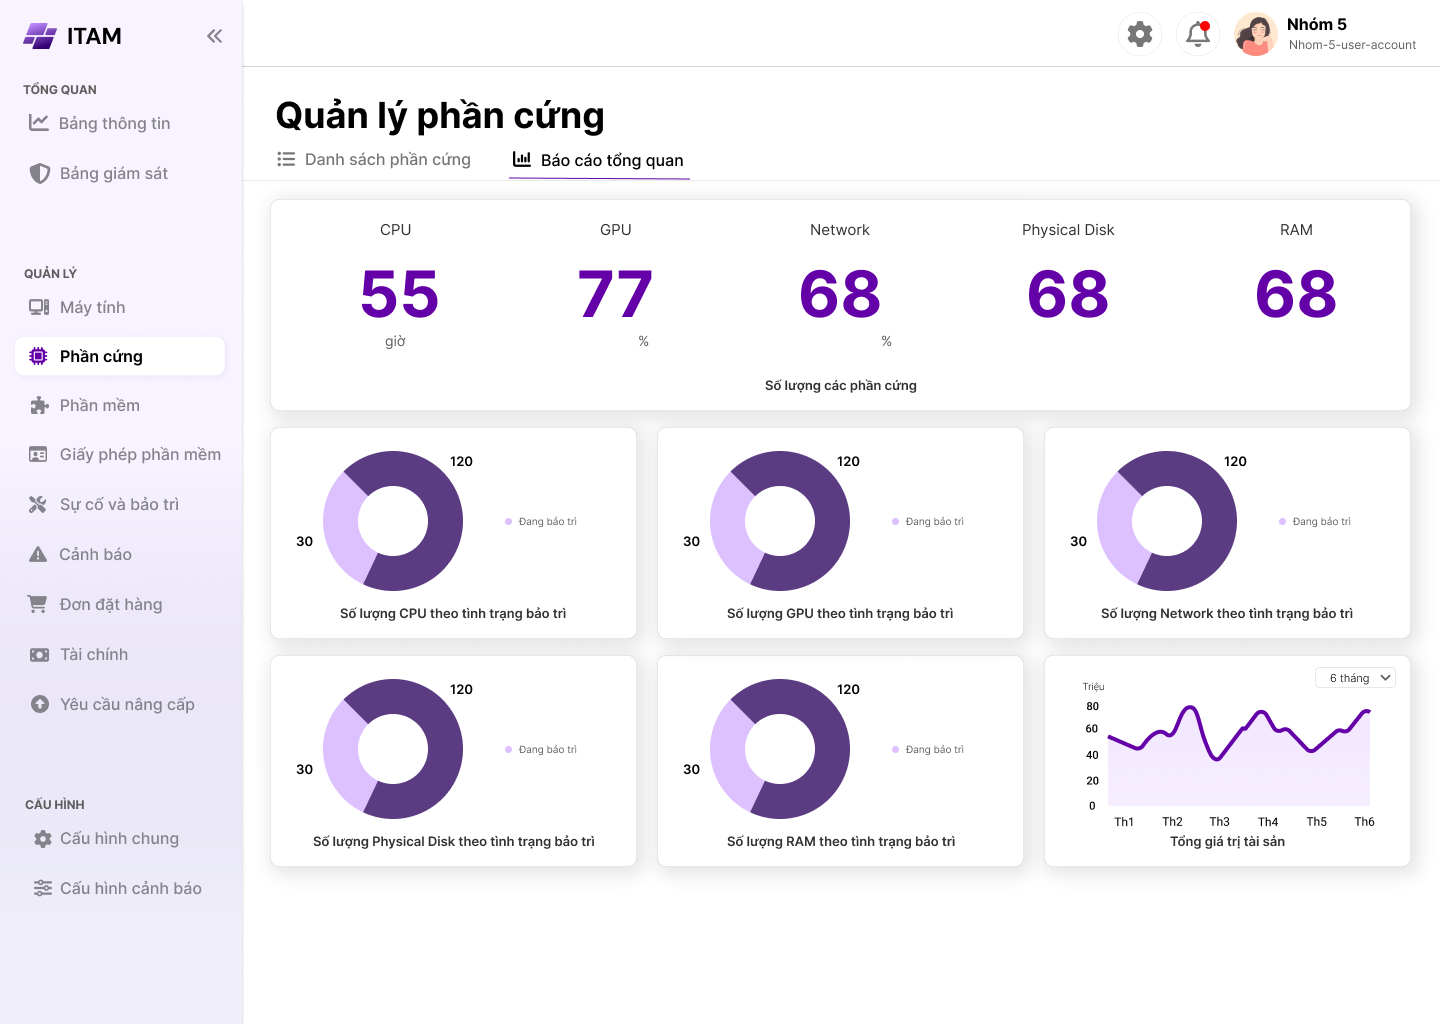
\includegraphics[width=14cm]{Images/C5/UI/Feature-Giám sát tài sản-Phần cứng 3.png}
        \vspace{15pt}
        \caption{Giao diện Quản lý phần cứng 4}
    \end{figure}

    \item{Quản lý phần mềm}\\
    \begin{figure}[H]
        \centering
        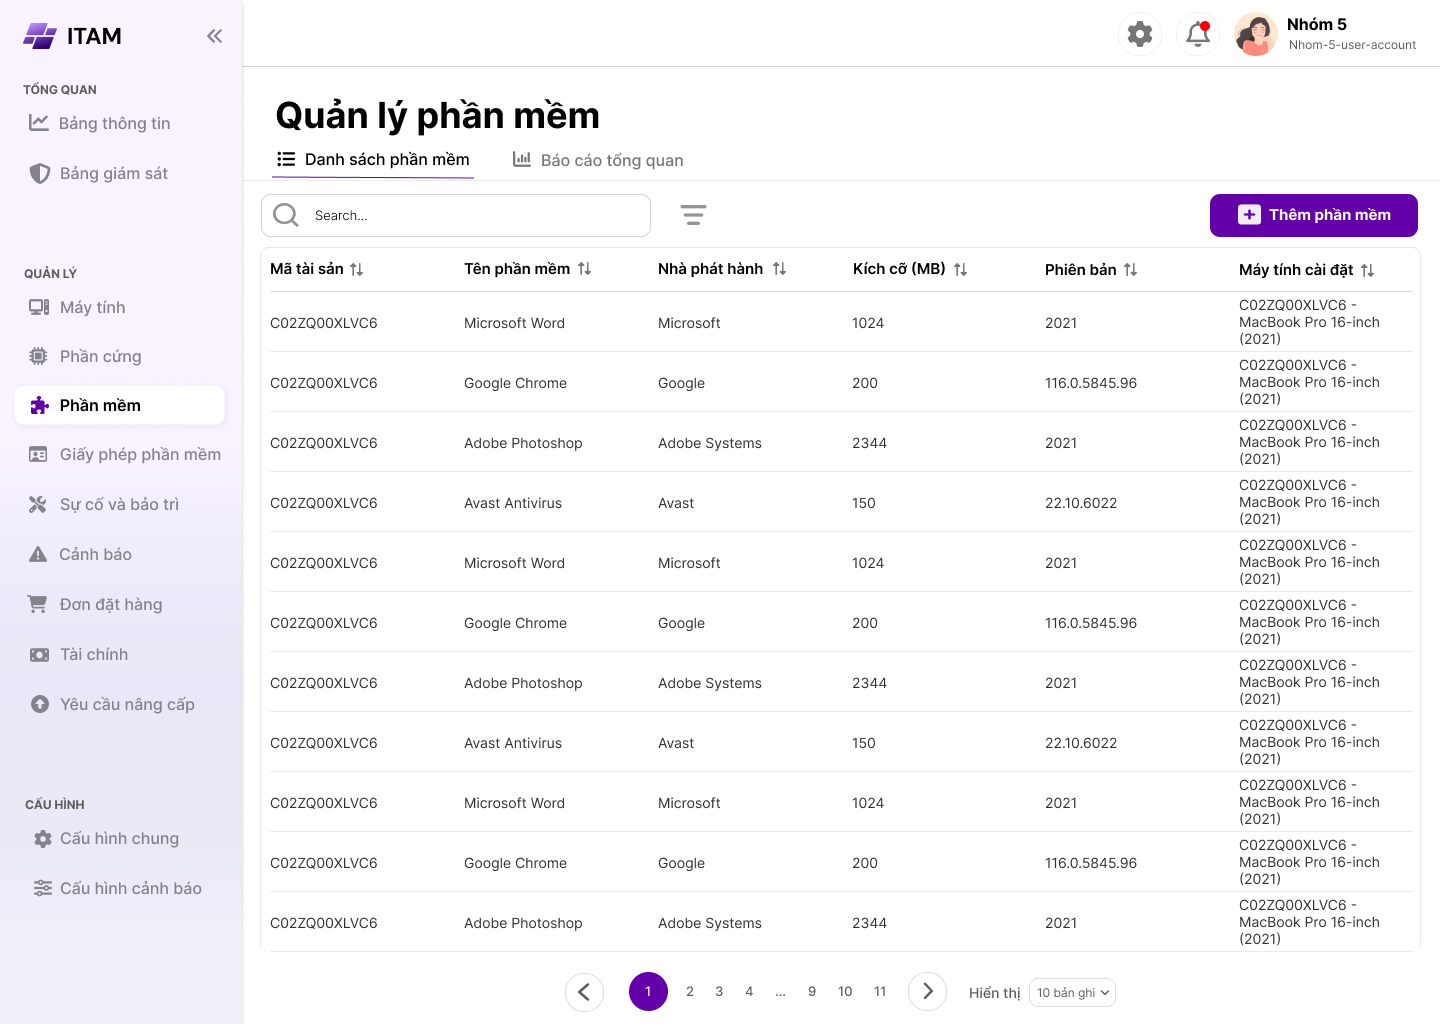
\includegraphics[width=14cm]{Images/C5/UI/Feature-Giám sát tài sản-Phần mềm 1.png}
        \vspace{15pt}
        \caption{Giao diện Quản lý phần mềm 1}
    \end{figure}
    \begin{figure}[H]
        \centering
        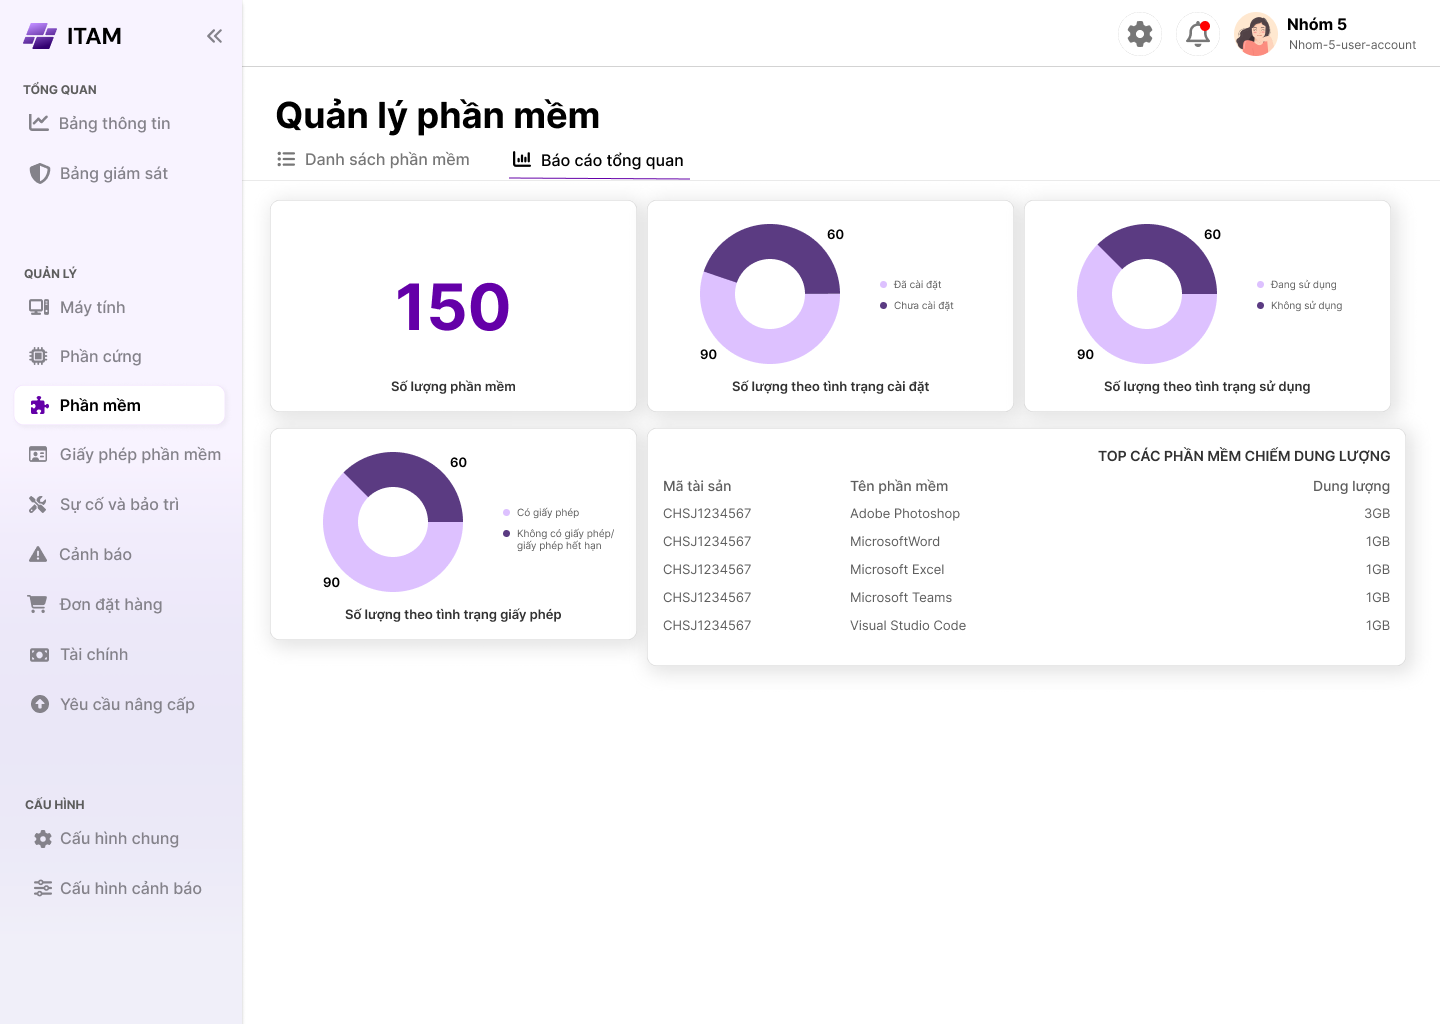
\includegraphics[width=14cm]{Images/C5/UI/Feature-Giám sát tài sản-Phần mềm 2.png}
        \vspace{15pt}
        \caption{Giao diện Quản lý phần mềm 2}
    \end{figure}
    \begin{figure}[H]
        \centering
        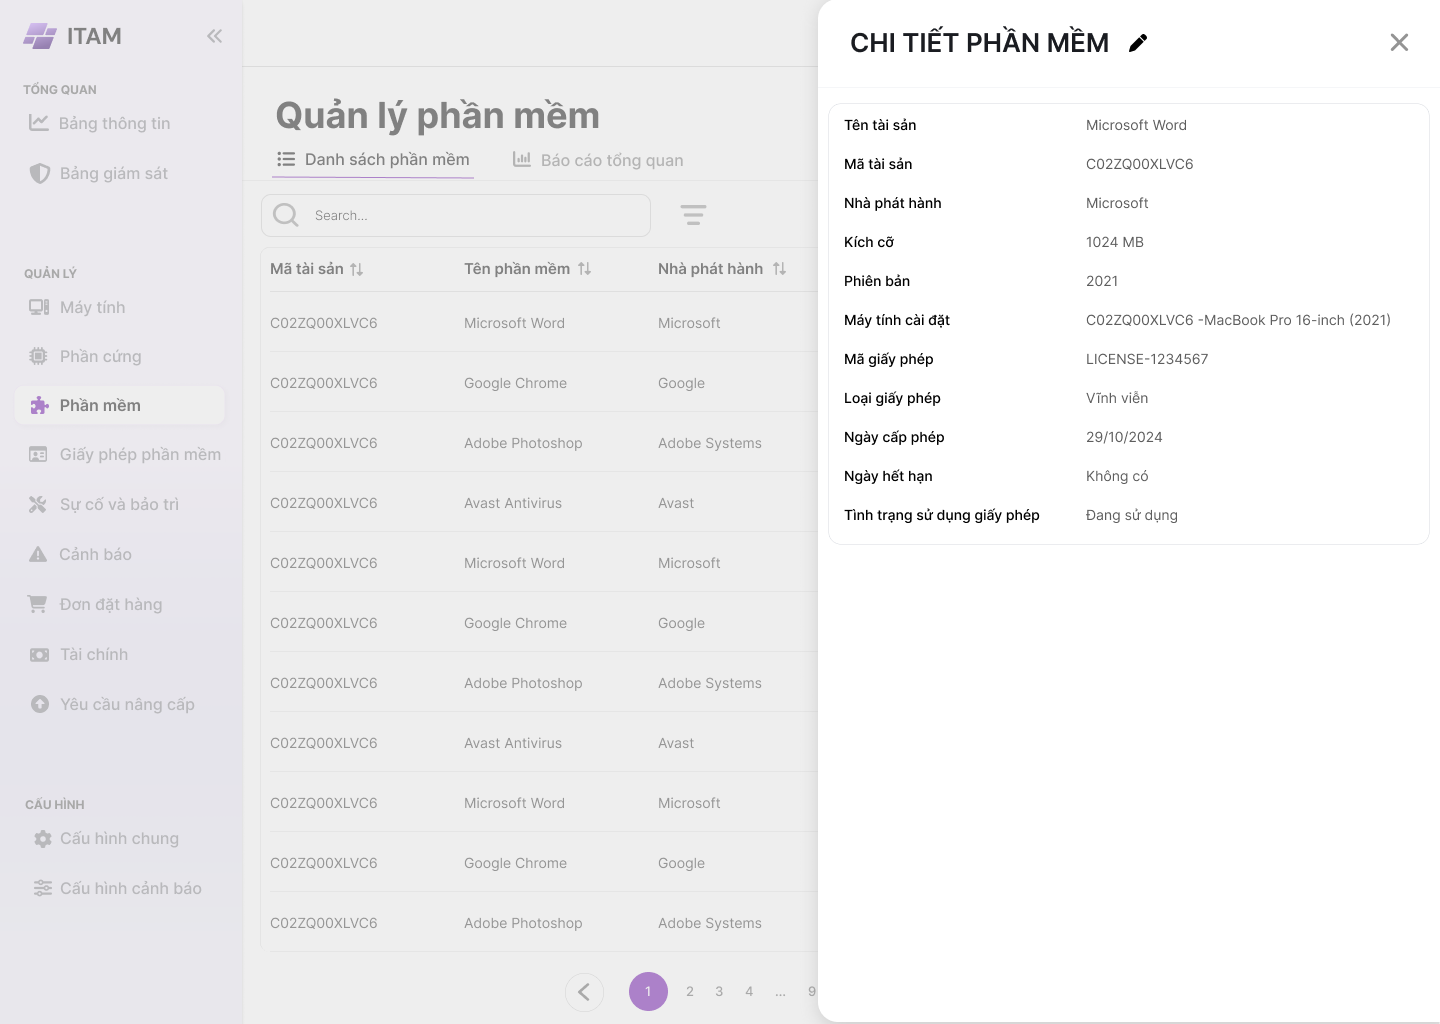
\includegraphics[width=14cm]{Images/C5/UI/Feature-Giám sát tài sản-Phần mềm 3.png}
        \vspace{15pt}
        \caption{Giao diện Quản lý phần mềm 3}
    \end{figure}
    \begin{figure}[H]
        \centering
        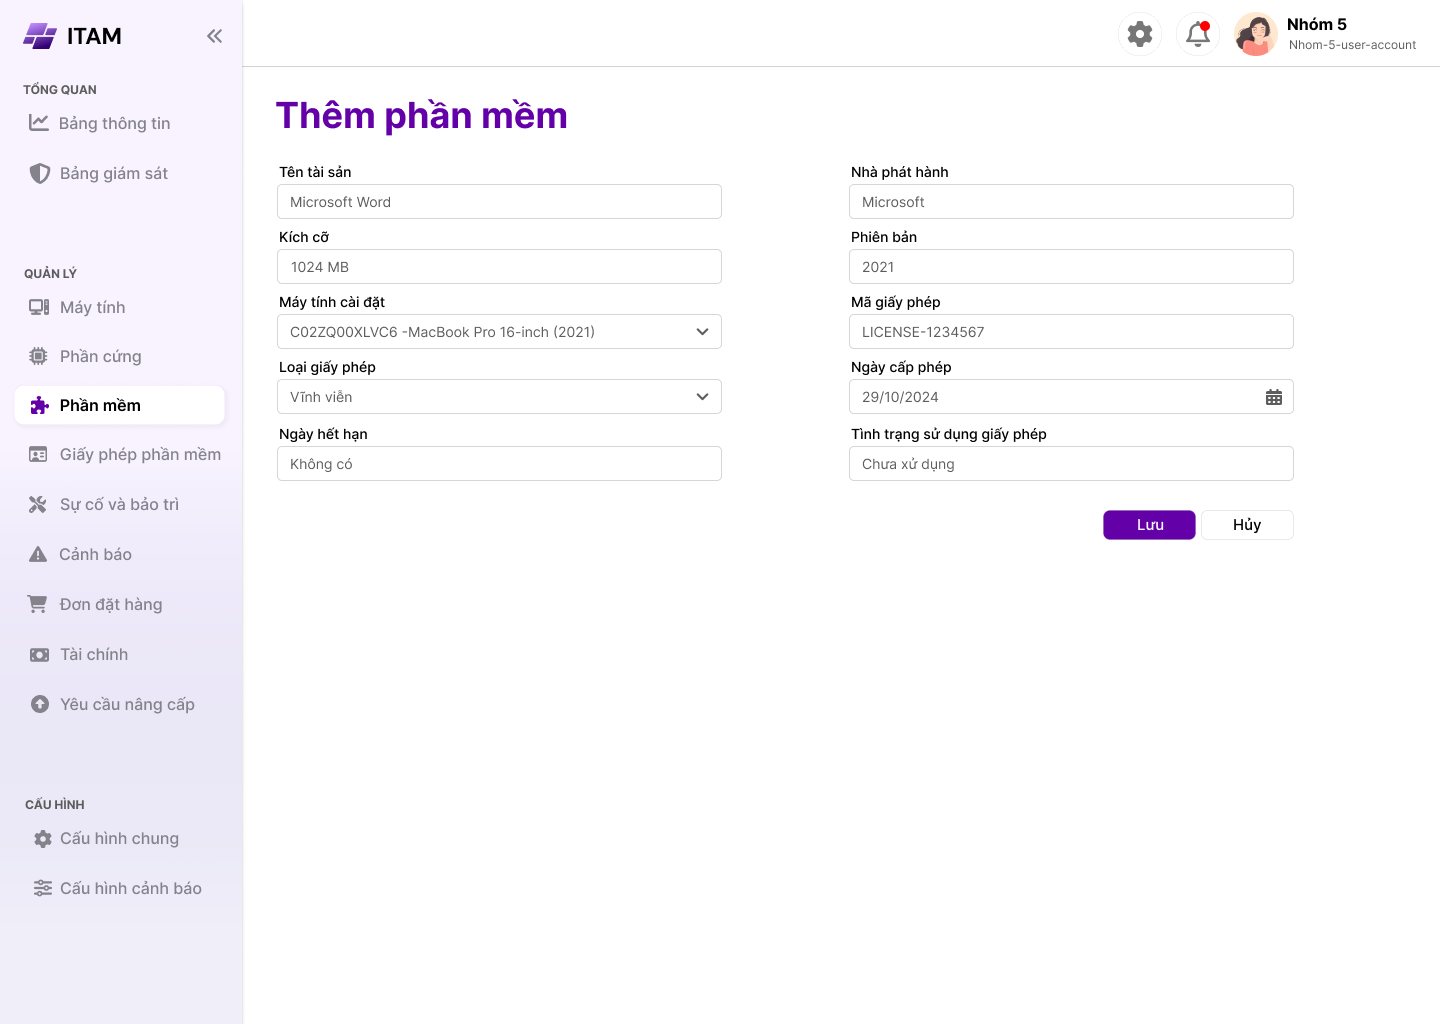
\includegraphics[width=14cm]{Images/C5/UI/Feature-Giám sát tài sản-Phần mềm 4.png}
        \vspace{15pt}
        \caption{Giao diện Quản lý phần mềm 4}
    \end{figure}

    \item{Quản lý sự cố và bảo trì}\\
    \begin{figure}[H]
        \centering
        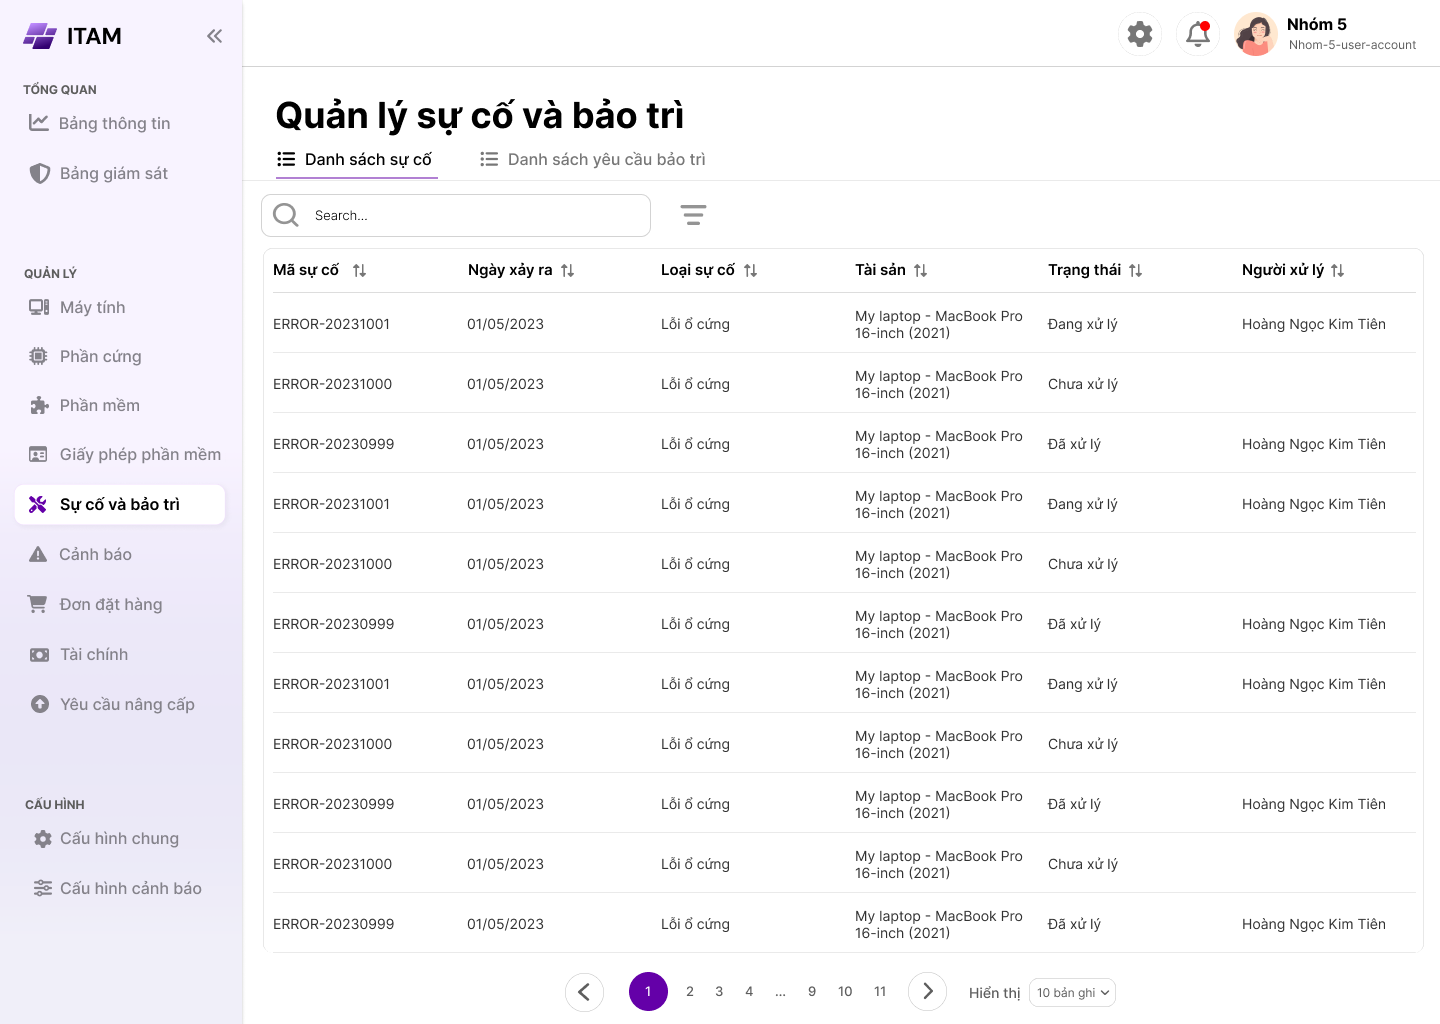
\includegraphics[width=14cm]{Images/C5/UI/Feature-Quản lý sự cố và bảo trì 1.png}
        \vspace{15pt}
        \caption{Giao diện Quản lý sự cố và bảo trì 1}
    \end{figure}
    \begin{figure}[H]
        \centering
        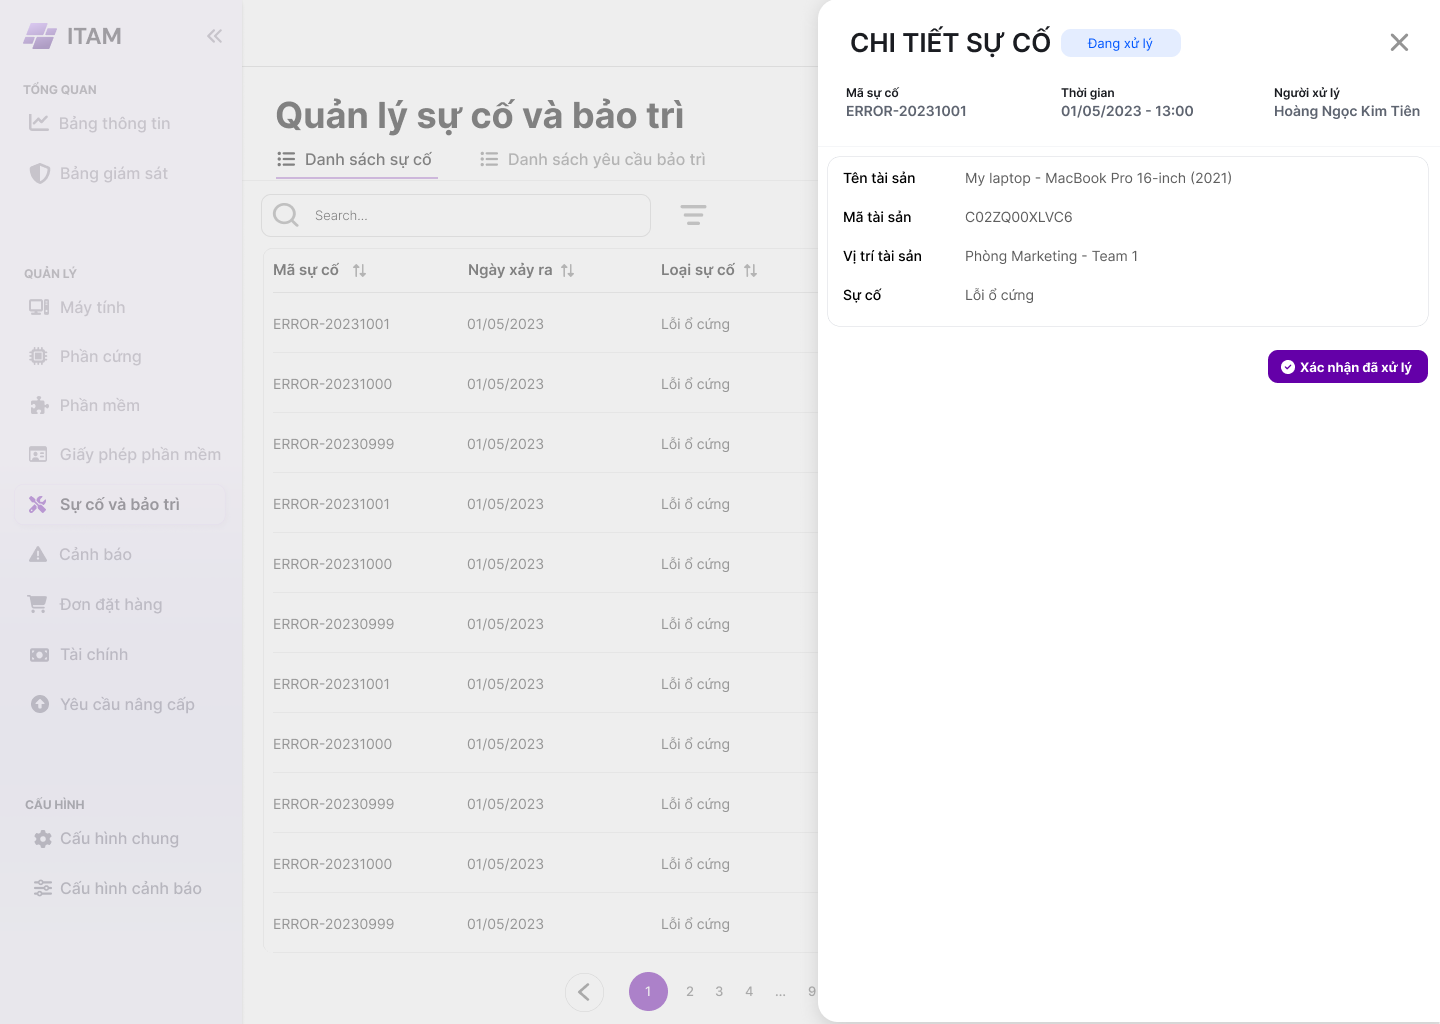
\includegraphics[width=14cm]{Images/C5/UI/Feature-Quản lý sự cố và bảo trì 2.1.png}
        \vspace{15pt}
        \caption{Giao diện Quản lý sự cố và bảo trì 2}
    \end{figure}
    \begin{figure}[H]
        \centering
        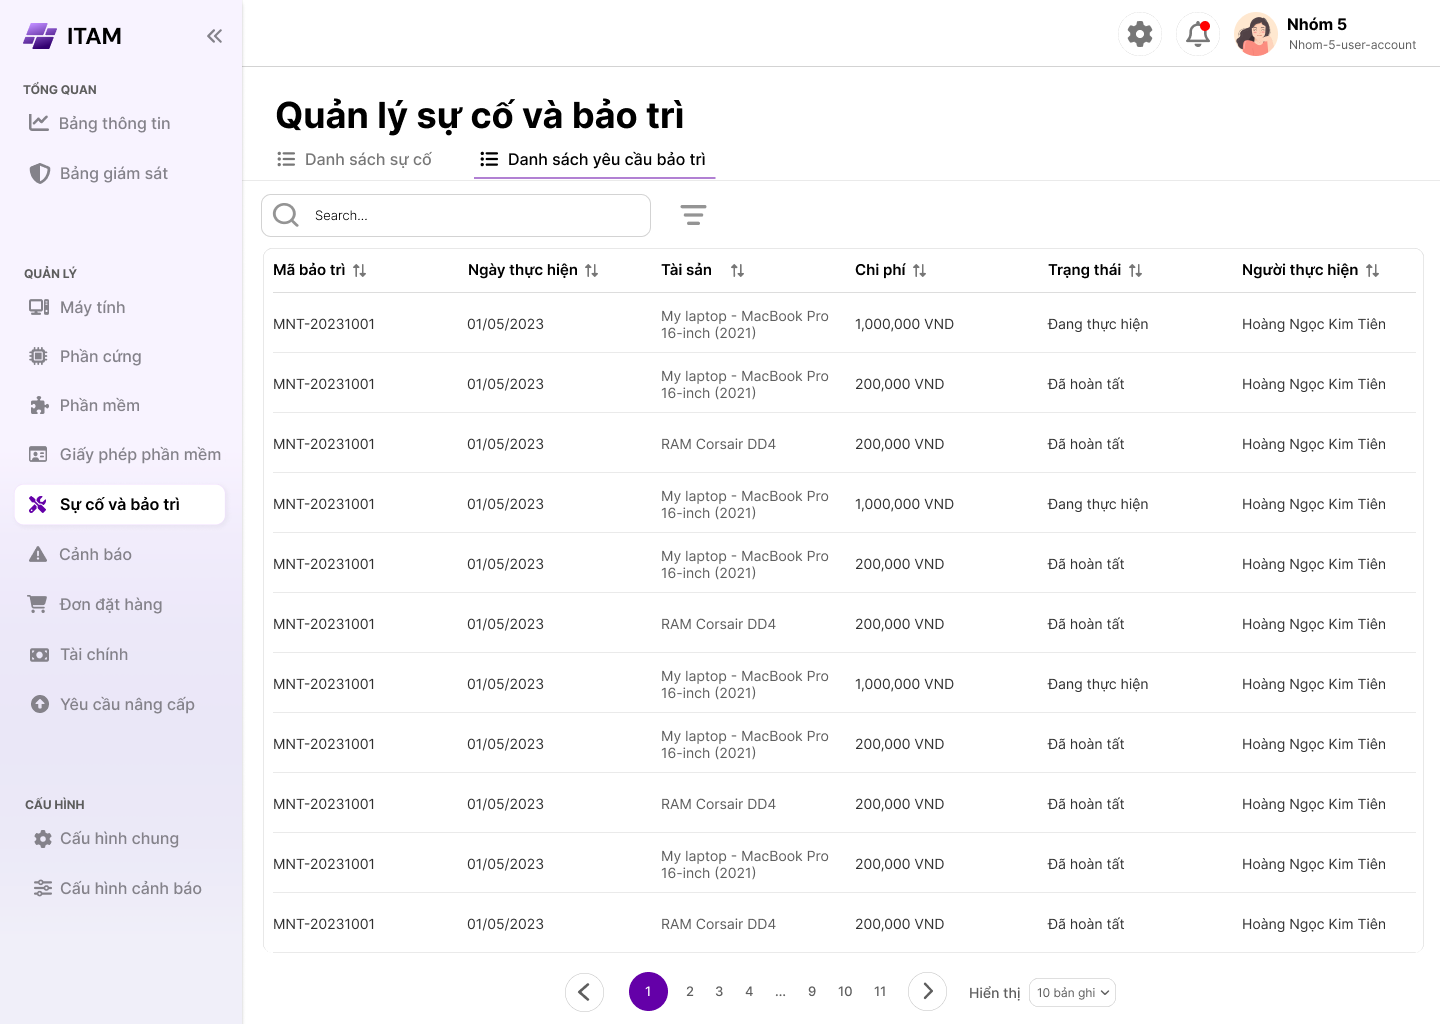
\includegraphics[width=14cm]{Images/C5/UI/Feature-Quản lý sự cố và bảo trì 3.1.png}
        \vspace{15pt}
        \caption{Giao diện Quản lý sự cố và bảo trì 3}
    \end{figure}
    \begin{figure}[H]
        \centering
        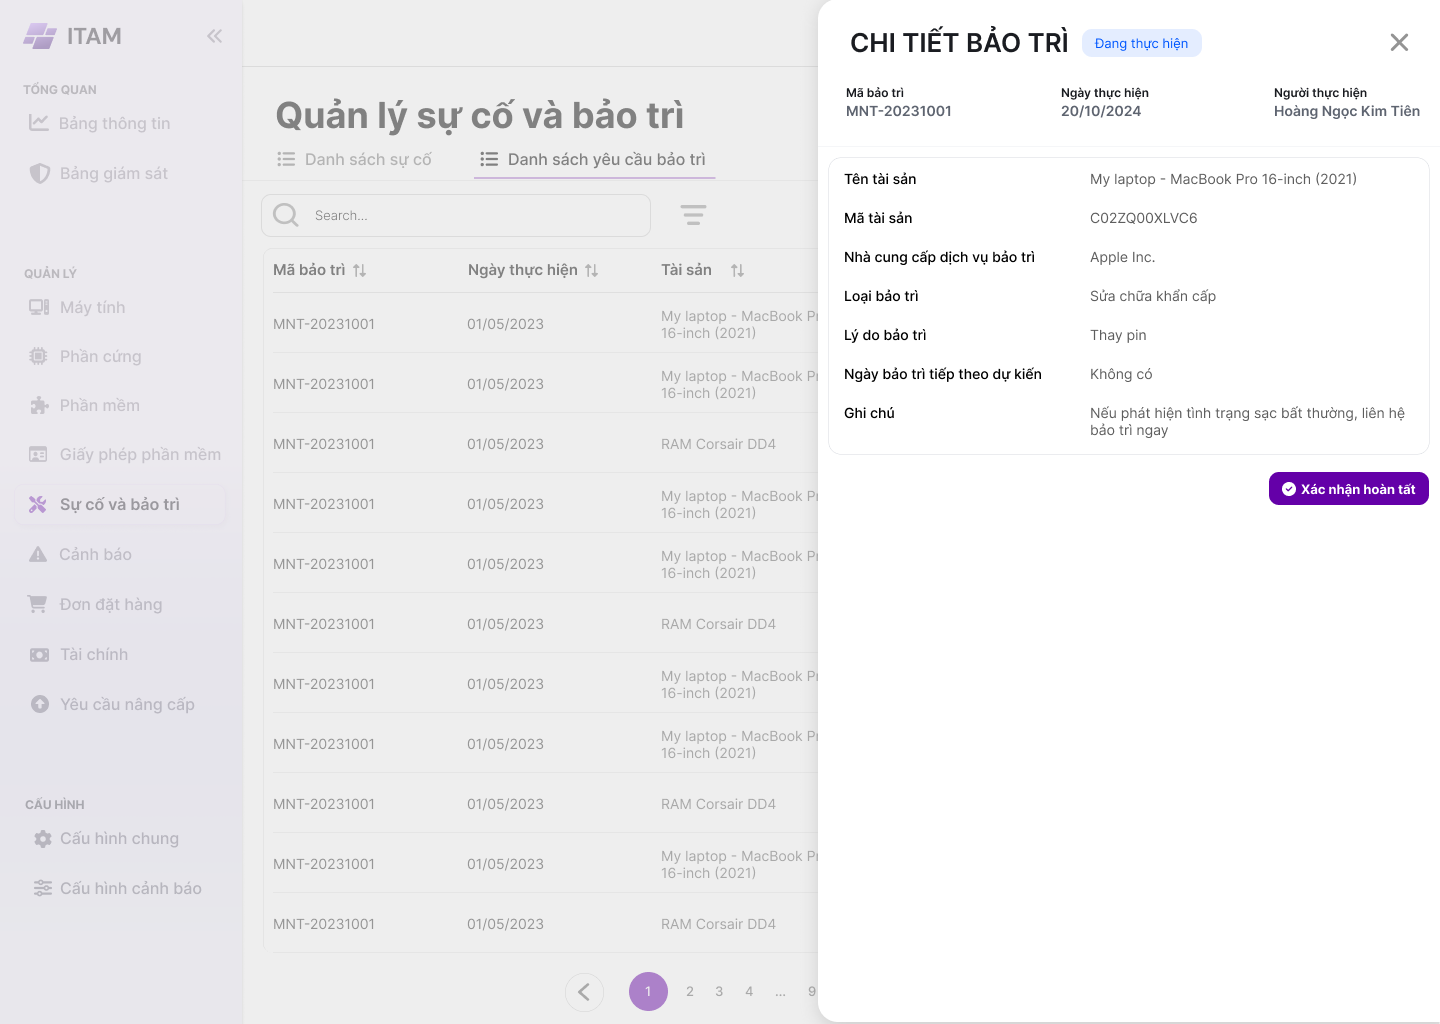
\includegraphics[width=14cm]{Images/C5/UI/Feature-Quản lý sự cố và bảo trì 3.2.png}
        \vspace{15pt}
        \caption{Giao diện Quản lý sự cố và bảo trì 4}
    \end{figure}

    \item{Quản lý cảnh báo}\\
    \begin{figure}[H]
        \centering
        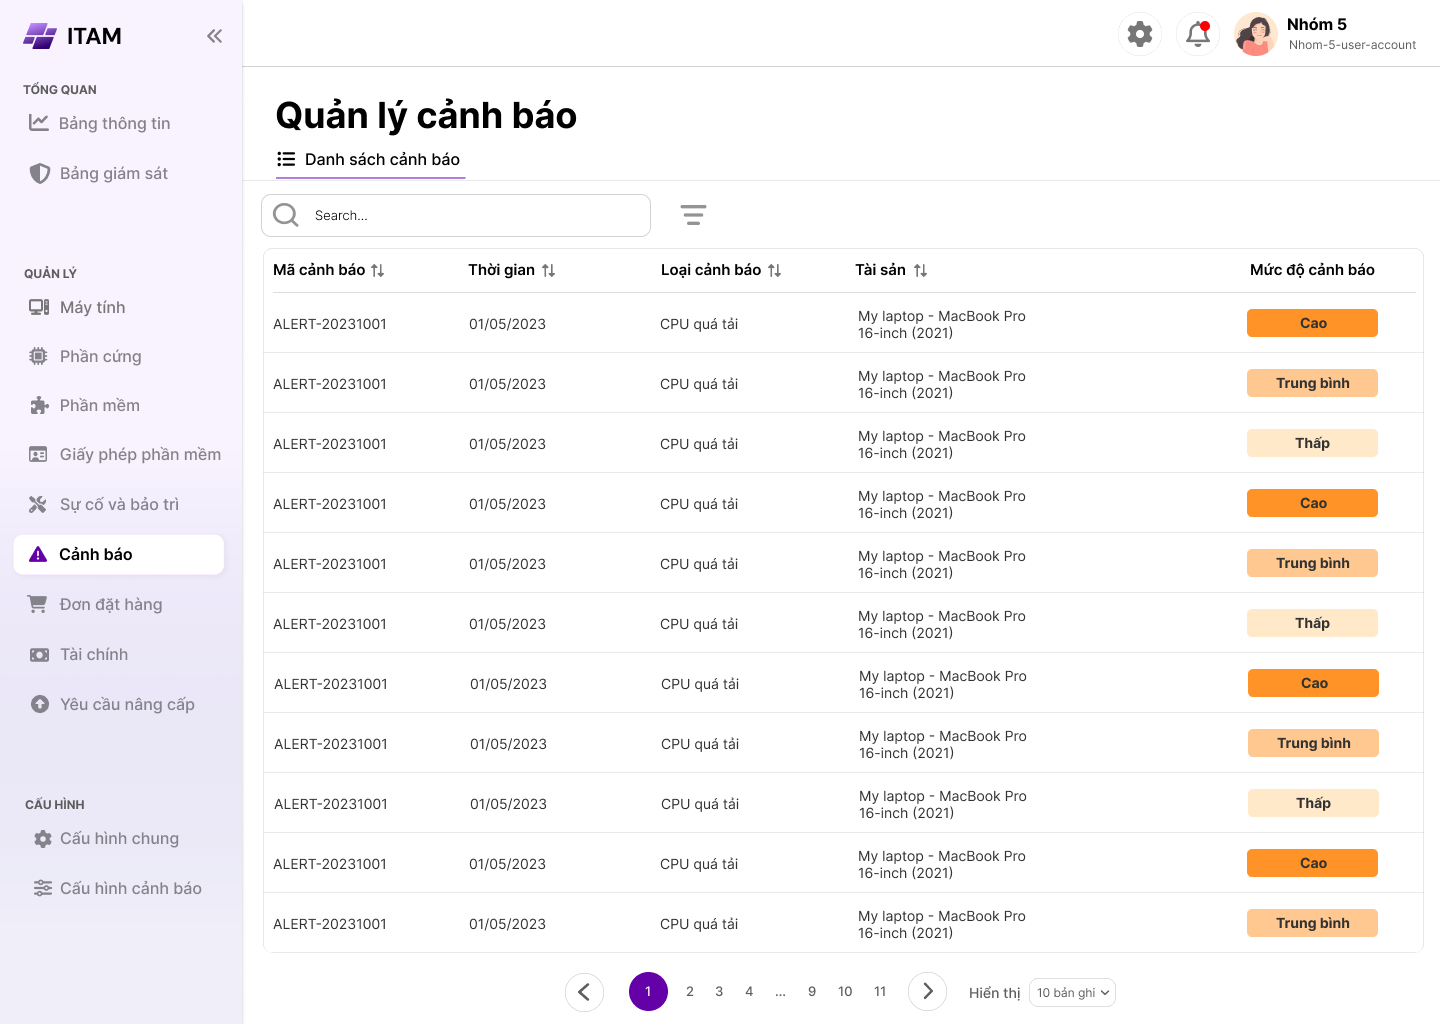
\includegraphics[width=14cm]{Images/C5/UI/Feature-Quản lý cảnh báo 1.png}
        \vspace{15pt}
        \caption{Giao diện Quản lý cảnh báo 1}
    \end{figure}
    \begin{figure}[H]
        \centering
        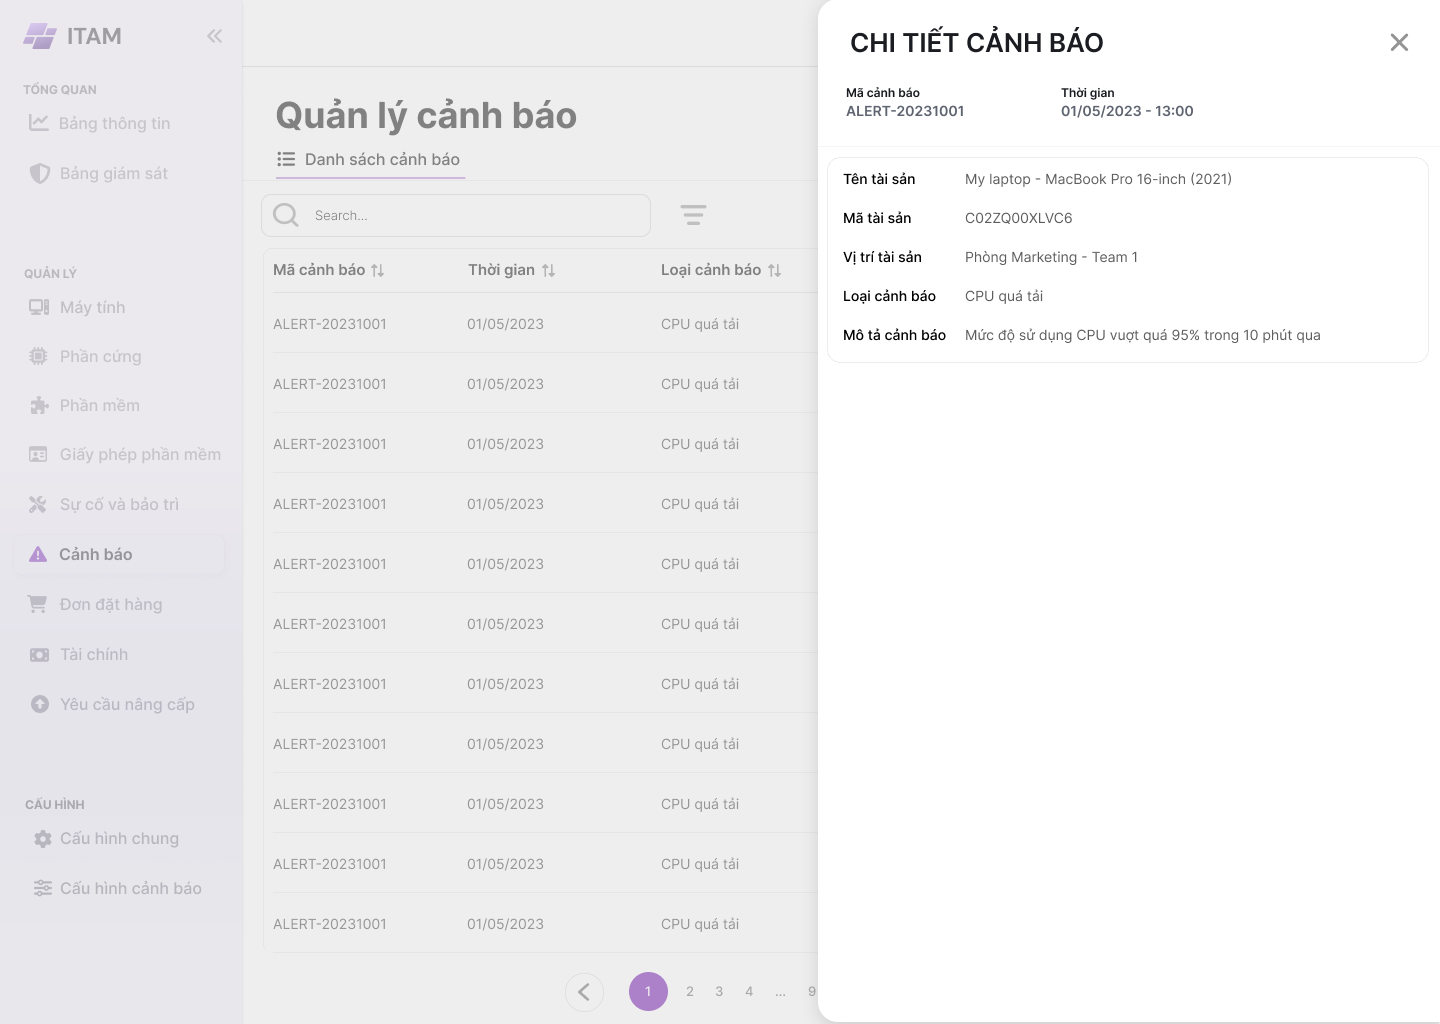
\includegraphics[width=14cm]{Images/C5/UI/Feature-Quản lý cảnh báo 2.1.png}
        \vspace{15pt}
        \caption{Giao diện Quản lý cảnh báo 2}
    \end{figure}

    \item{Quản lý yêu cầu nâng cấp}\\
    \begin{figure}[H]
        \centering
        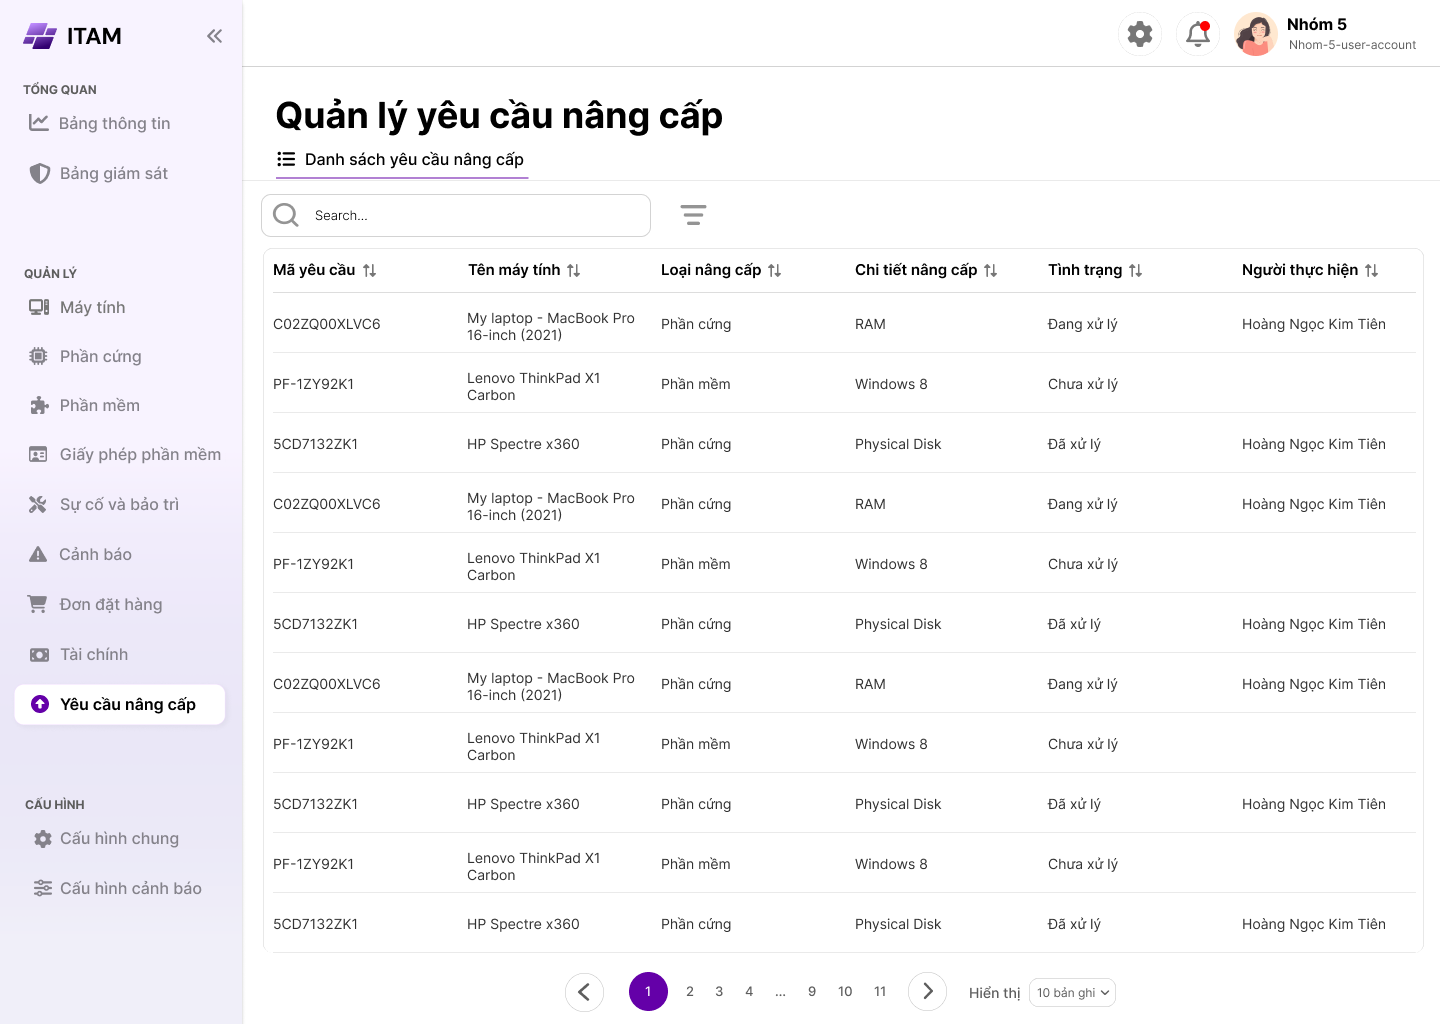
\includegraphics[width=14cm]{Images/C5/UI/Feature-Quản lý yêu cầu nâng cấp 1.png}
        \vspace{15pt}
        \caption{Giao diện Quản lý yêu cầu nâng cấp 1}
    \end{figure}
    \begin{figure}[H]
        \centering
        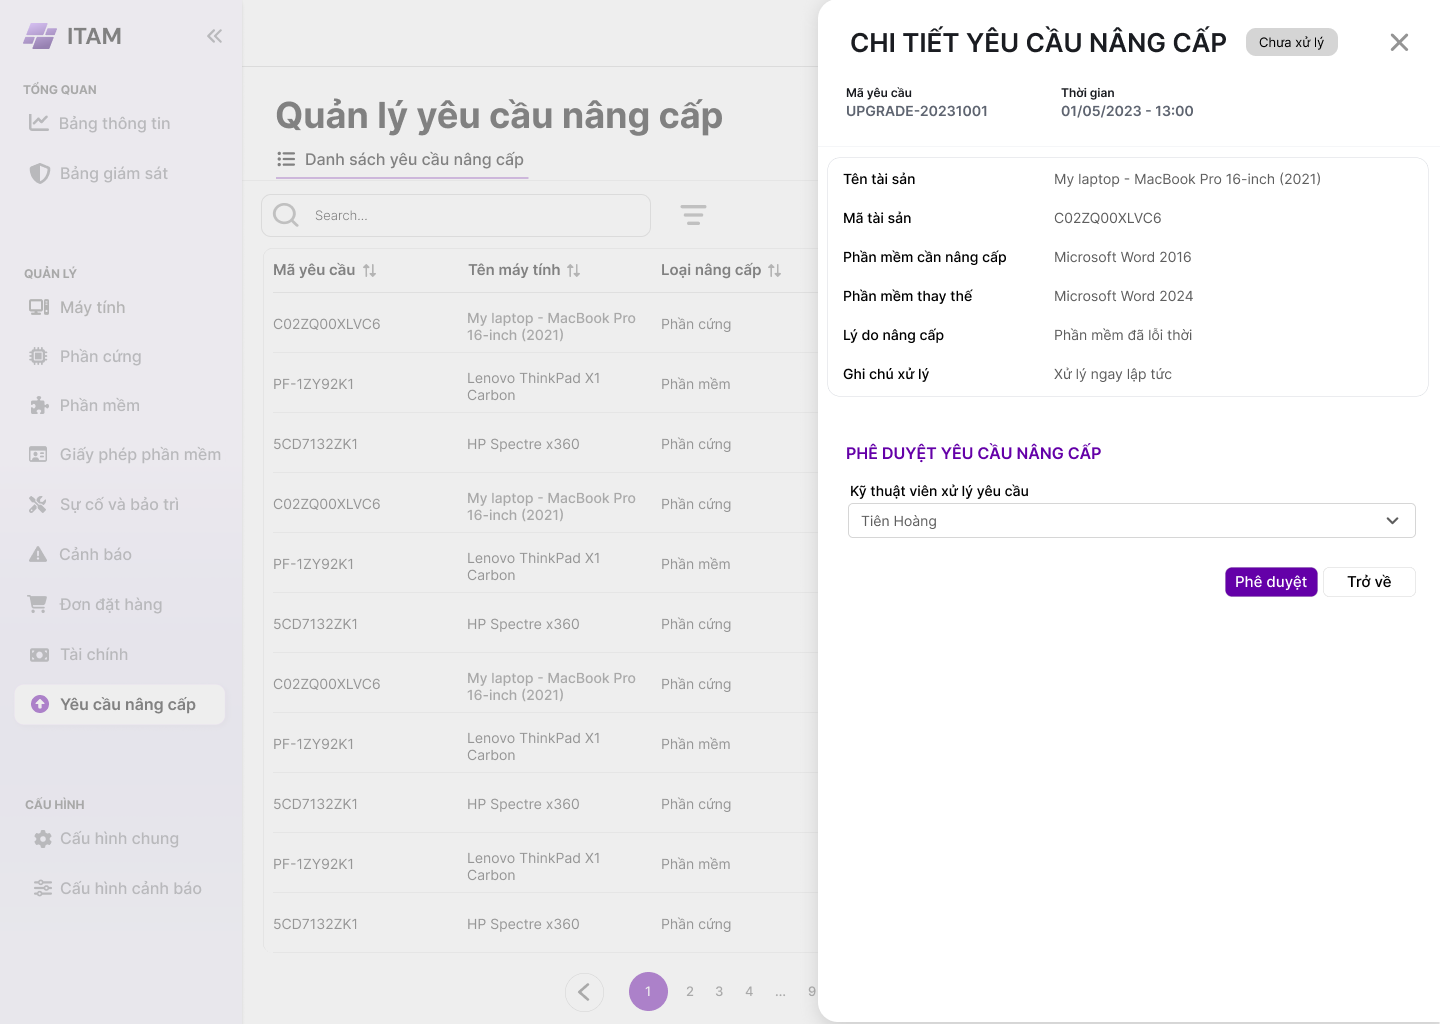
\includegraphics[width=14cm]{Images/C5/UI/Feature-Quản lý yêu cầu nâng cấp 2.4.png}
        \vspace{15pt}
        \caption{Giao diện Quản lý yêu cầu nâng cấp 2}
    \end{figure}

    \item{Quản lý đơn đặt hàng}\\
    \begin{figure}[H]
        \centering
        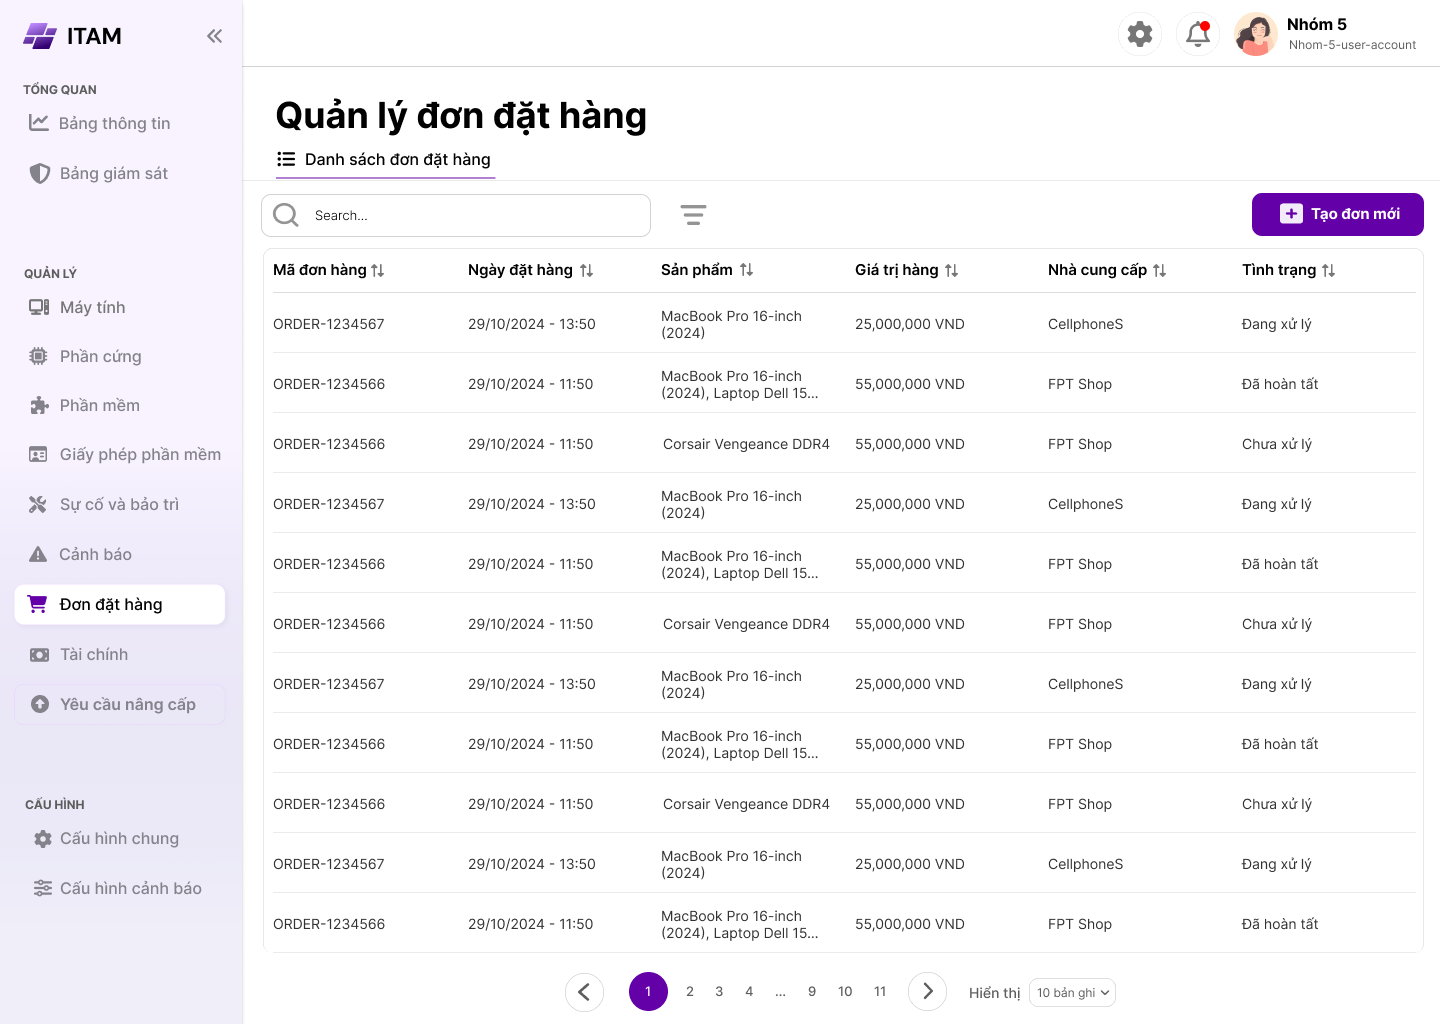
\includegraphics[width=14cm]{Images/C5/UI/Feature-Quản lý đơn đặt hàng 1.png}
        \vspace{15pt}
        \caption{Giao diện Quản lý đơn đặt hàng 1}
    \end{figure}
    \begin{figure}[H]
        \centering
        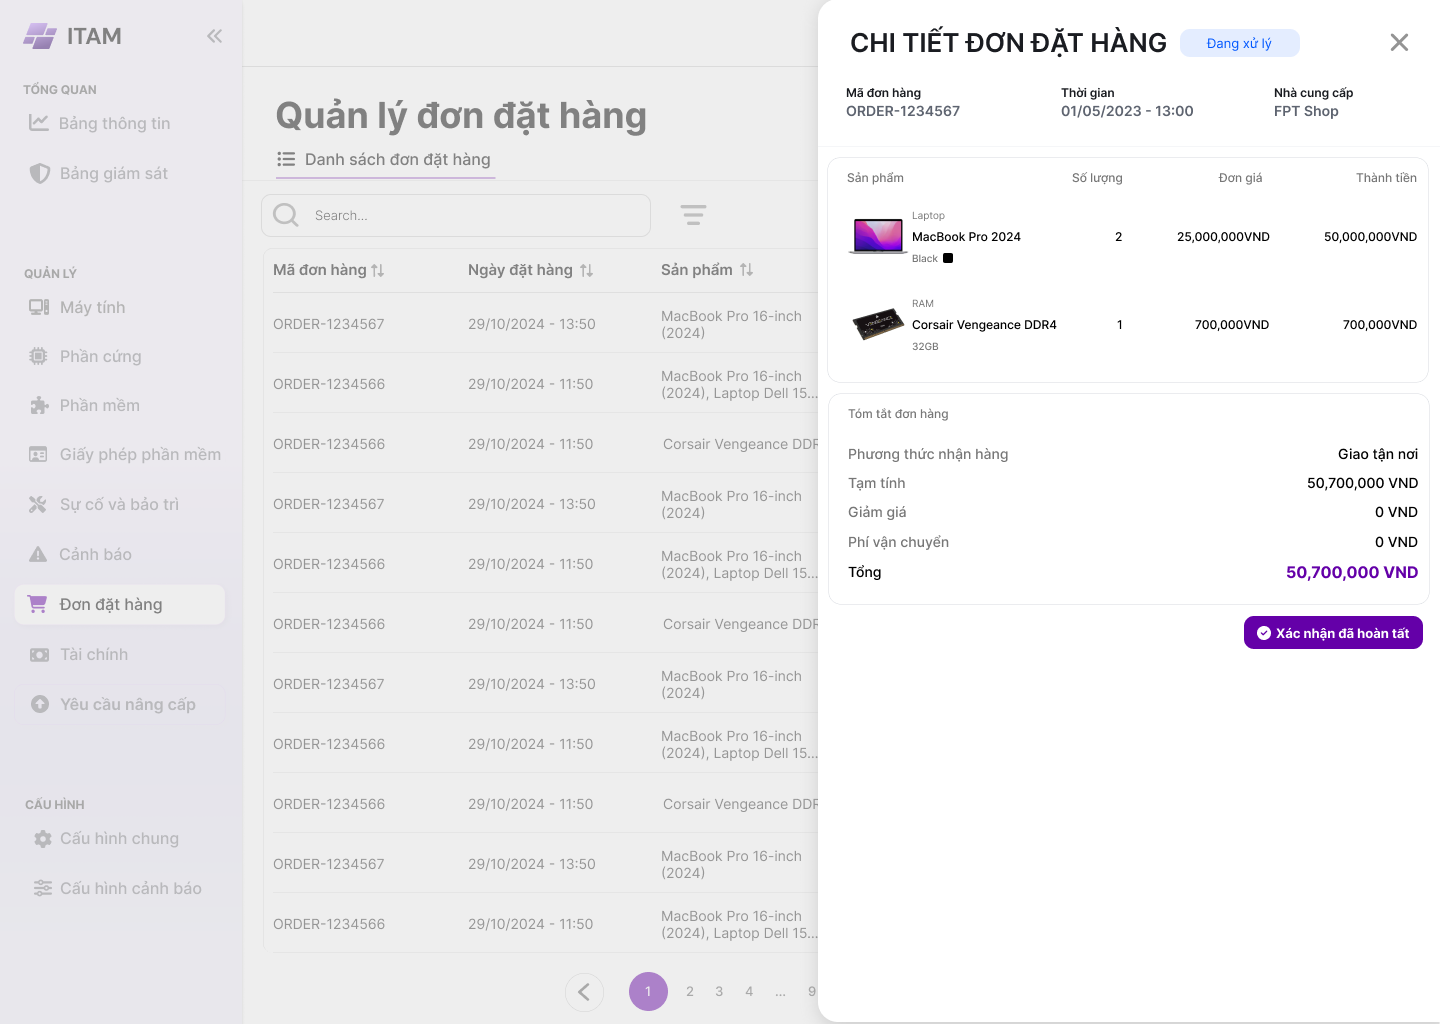
\includegraphics[width=14cm]{Images/C5/UI/Feature-Quản lý đơn đặt hàng 2.1.png}
        \vspace{15pt}
        \caption{Giao diện Quản lý đơn đặt hàng 2}
    \end{figure}
    \begin{figure}[H]
        \centering
        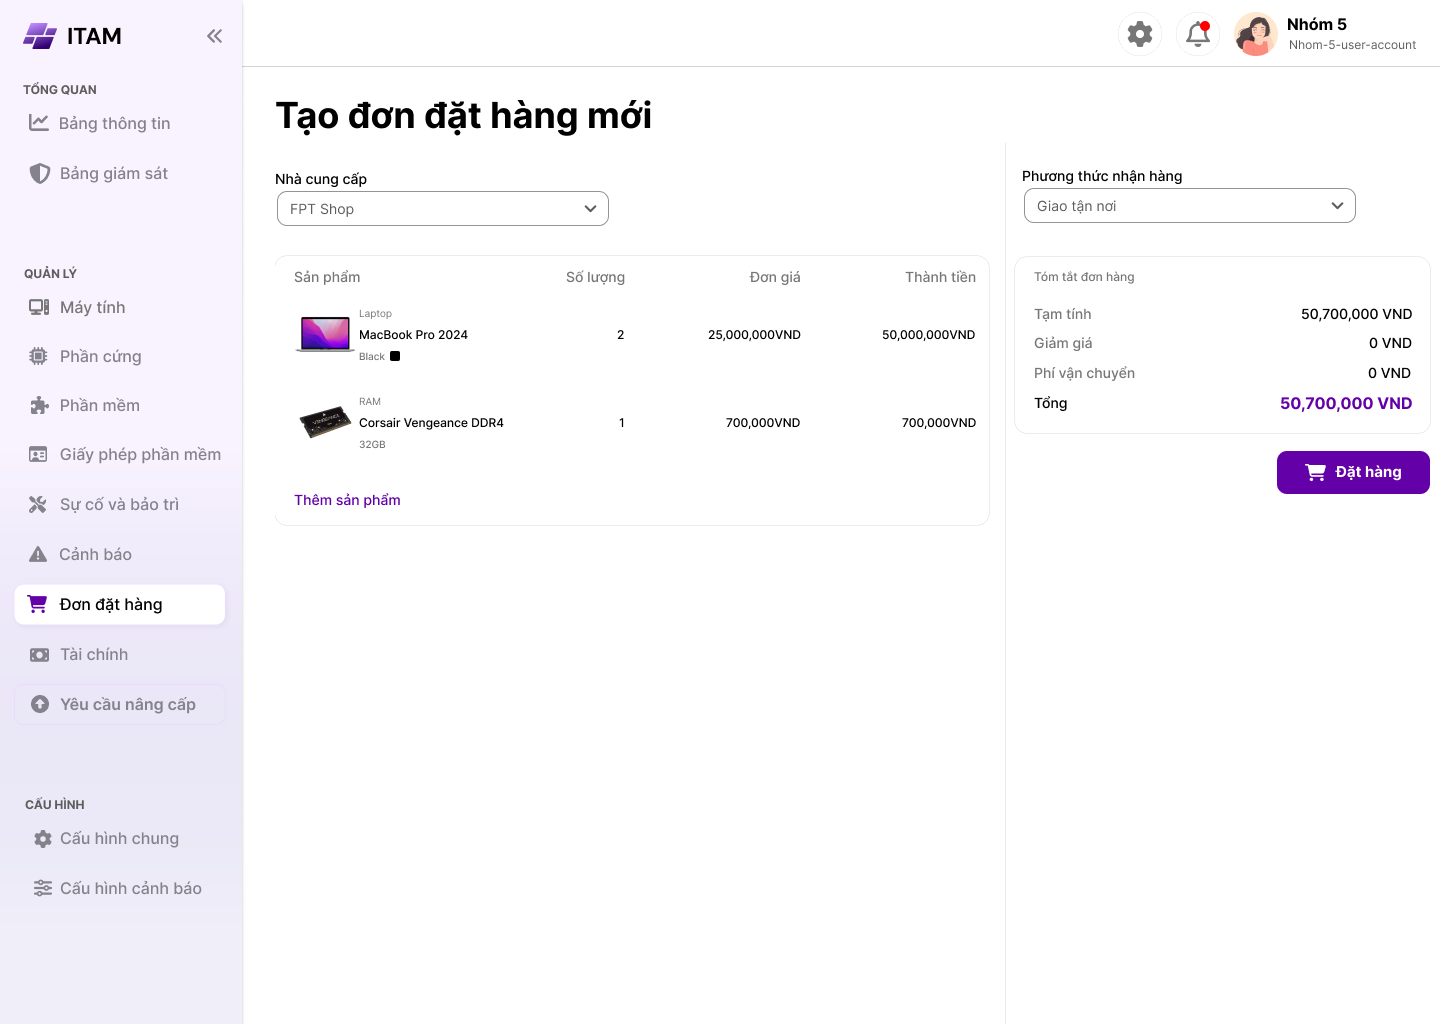
\includegraphics[width=14cm]{Images/C5/UI/Feature-Quản lý đơn đặt hàng 3.1.png}
        \vspace{15pt}
        \caption{Giao diện Quản lý đơn đặt hàng 3}
    \end{figure}

    \item{Quản lý giấy phép phần mềm}\\
    \begin{figure}[H]
        \centering
        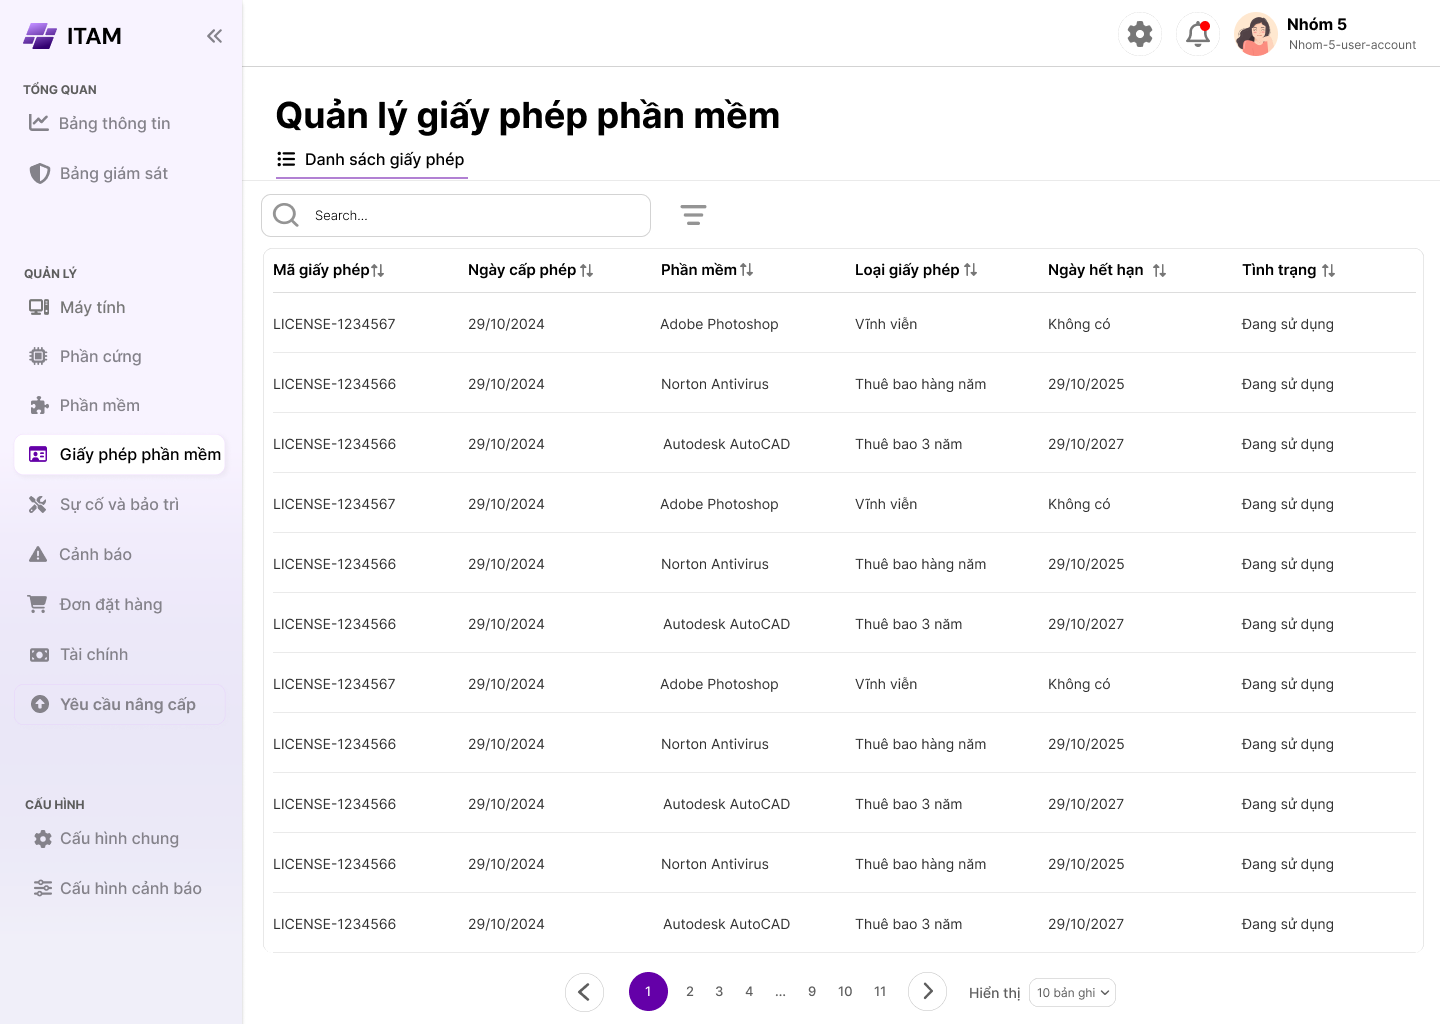
\includegraphics[width=14cm]{Images/C5/UI/Feature-Quản lý giấy phép phần mềm.png}
        \vspace{15pt}
        \caption{Giao diện Quản lý giấy phép phần mềm}
    \end{figure}

    \item{Quản lý cấu hình cảnh báo}\\
    \begin{figure}[H]
        \centering
        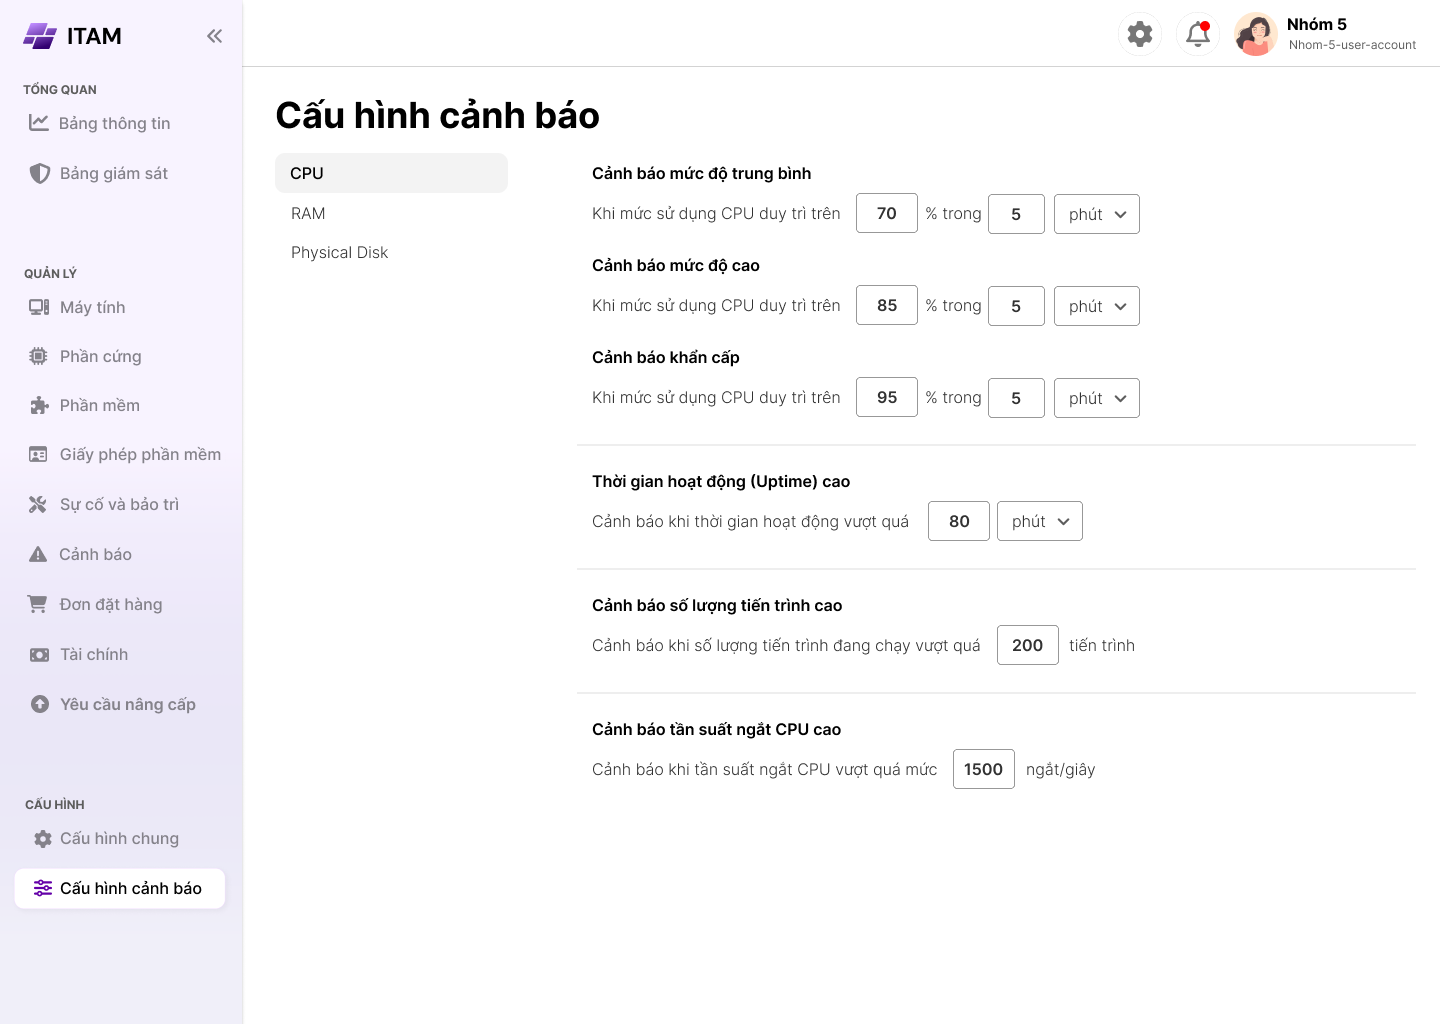
\includegraphics[width=14cm]{Images/C5/UI/Feature-Cấu hình cảnh báo 1.png}
        \vspace{15pt}
        \caption{Giao diện Quản lý cấu hình cảnh báo 1}
    \end{figure}
    \begin{figure}[H]
        \centering
        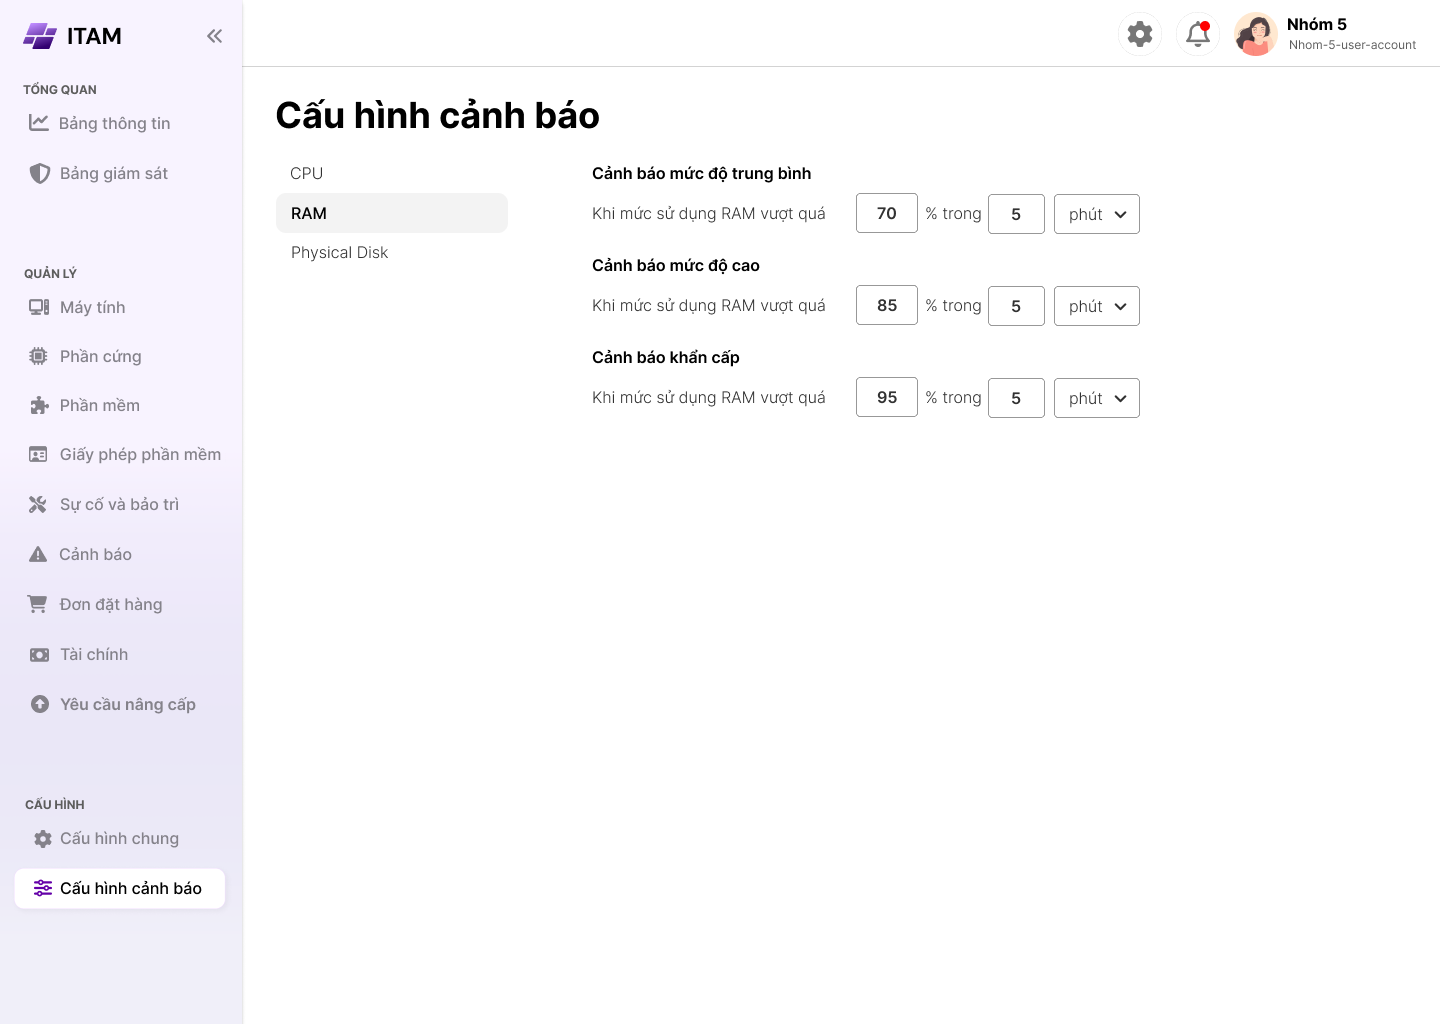
\includegraphics[width=14cm]{Images/C5/UI/Feature-Cấu hình cảnh báo 5.png}
        \vspace{15pt}
        \caption{Giao diện Quản lý cấu hình cảnh báo 2}
    \end{figure}
    \begin{figure}[H]
        \centering
        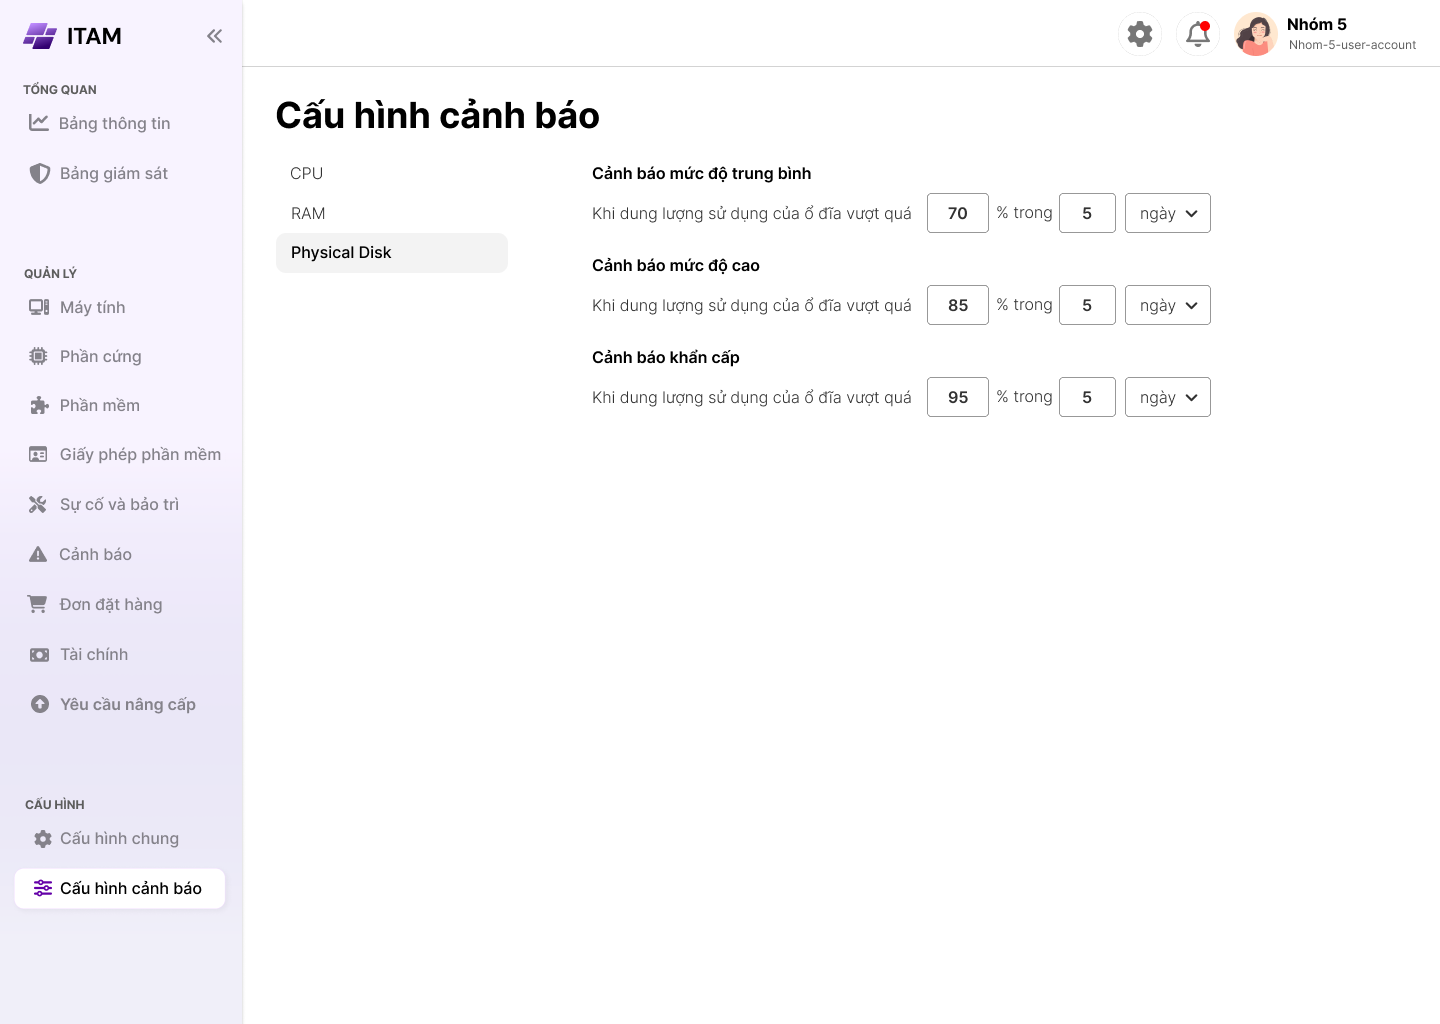
\includegraphics[width=14cm]{Images/C5/UI/Feature-Cấu hình cảnh báo 6.png}
        \vspace{15pt}
        \caption{Giao diện Quản lý cấu hình cảnh báo 3}
    \end{figure}
\end{itemize}
%%%%%%%%%%%%%%%%%%%%%%%%%%%%%%%%%%%%%%%%%%%%%%%%%%%%%%%%%%%%
\section{Phụ lục Mô tả Class Diagram}
\begin{enumerate}
    %%%%%%%%%
    \item Lớp User\\
     Các Thuộc tính:
    \begin{itemize}[label=--]
        \item Username: String (Public)
        \item Password: String(Protected)
        \item Email: String (Protected)
        \item EmployeeID: String (Protected)
        \item PhoneNumber: String (Protected)
        \item Role: String
        \item DateCreated: Datetime
        \item LoginHistorys: List<LoginHistory>
    \end{itemize}
    Phương thức:
    \begin{itemize}[label=--]
        \item getUserInfo(userID: String):  User
        \item getUserRole():String
        \item viewLoginHistory(): List<LoginHistory>
    \end{itemize}
    Mối quan hệ: Lớp Admin, ITStaff, Manager kế thừa từ lớp Admin
    %%%%%%%%%
    \item Lớp Admin: Kế thừa từ lớp User\\
    Phương thức:
    \begin{itemize}[label=--]
        \item createUser(username: String, password: String, employeeID: String, phoneNumber: String, email: String, role: String): Boolean
        \item generateEmployeeID(): string
        \item updateUser(username: String, password: String, employeeID: String, phoneNumber: String, email: String, role: String): Boolean
        \item deleteUser():Boolean
    \end{itemize}
    %%%%%%%%%%%%%%%5
    \item Lớp Manager: Kế thừa từ lớp User\\
    Các Thuộc tính:
    \begin{itemize}[label=--]
        \item ManagerID : String (Public)
        \item PurchaseOrders: List<PurchaseOrder> (Public)
        \item UpgradeRequests: List<UpgradeRequest> (Public)
    \end{itemize}
    Phương thức:
    \begin{itemize}[label=--]
        \item createPurchaseOrder(): Boolean
        \item removePurchaseOrder(): Boolean
        \item approveUpgradeRequest(UpgradeRequest):Boolean
        \item getSupplierInfo(): List<Supplier>
    \end{itemize}
    Mối quan hệ tham gia:
    \begin{itemize}[label=--]
        \item Association với lớp UpgradeRequest
        \item Composition với lớp PurchaseOrder
    \end{itemize}
    %%%%%%%%%%%%%%%%%%%%%%%%%%
    \item Lớp ITStaff: Kế thừa từ lớp User
    Các thuộc tính:
    \begin{itemize}[label=--]
        \item ITStaffID: String
        \item Maintenances: List<Maintenance>
        \item Thresholds: List<Threshold>
        \item Errors: List<Error>
        \item AssetAssignments: List<AssetAssignment>
        \item UpgradeRequests: List<UpgradeRequest>
    \end{itemize}
    Phương thức:
    \begin{itemize}[label=--]
        \item assignAsset(asset: Asset, assignmentDate: Datetime): Boolean
        \item releaseAsset(asset: Asset, returnDate: Datetime): Boolean
        \item listAssignedAssets(): List<Asset>
        \item createMaintenance(assetID: String): Boolean
        \item listMaintenance(): List<Maintenance>
        \item handleError(error: Error,handleDate: Datetime): Boolean
        \item modifyThreshold(threshold: Threshold,ModifyDate: Datetime): Boolean
        \item createUpgradeRequest(List<Asset>): Boolean
    \end{itemize}
    Mối quan hệ tham gia:
    \begin{itemize}[label=--]
        \item Association với lớp Error, Threshold, Implementation
        \item Compostion với lớp upgradeRequest, Maintenance
        \item Aggregation với lớp AssetAssignment
    \end{itemize}
    \item Lớp UpgradeRequest:\\
    Các thuộc tính:
    \begin{itemize}[label=--]
        \item RequestID: String
        \item ITStaffID: String
        \item ManagerID:String
        \item Type: String
        \item CreatedDate: Datetime
        \item Description: String
        \item ApprovalTime: Datetime
        \item Approved: Boolean
        \item PurchaseOrders: List<PurchaseOrder>
    \end{itemize}
    Phương thức:
    \begin{itemize}[label=--]
        \item setApproval(approved: Boolean, approvalTime: Datetime, requestId: String): Boolean
        \item updateRequestDetail(request: UpgradeRequest): Boolean
        \item getRequestDetail(): UpgradeRequest
    \end{itemize}
    Mối quan hệ tham gia:
    \begin{itemize}[label=--]
        \item Compostion với lớp AssetUpgrade
        \item Compostion với lớp ITStaff
    \end{itemize}
    \item Lớp Asset\\
    Các thuộc tính:
    \begin{itemize}[label=--]
        \item AssetID: String
        \item Name: String
    \end{itemize}
    Phương thức:
    \begin{itemize}[label=--]
        \item GetAllAssets(): List<Asset>
        \item  CreateAssetAsync(asset: AssetDto): Asset
        \item UpdateAsset(Id: string, asset: AssetDto): Asset
        \item DeleteAsset(Id: string): Bool  
    \end{itemize}
    Mối quan hệ tham gia:
    \begin{itemize}[label=--]
        \item Aggregation với lớp AssetUpgrade, AssetAssignment
        \item Compostion với lớp Error
        \item Association với lớp Maintenance, Disposal, Implementation, Utilization, DisposalRequest, Procurement
    \end{itemize}
    \item Lớp AssetAssignment: Lớp trung gian cho mối quan hệ nhiều nhiều giữa Asset và ITStaff
    Các phương thức:
    \begin{itemize}[label=--]
        \item assignAsset(staff: ITStaff, asset: Asset): Boolean
        \item ExtendDate( extendDate: Datetime) : Boolean 
    \end{itemize}
    Tham gia mối quan hệ Aggregation với lớp ITStaff và lớp Asset
    %%%%%%%%%%%%%
    \item Lớp AssetUpgrade: Lớp trung gian cho mối quan hệ nhiều nhiều giữa Asset và UpgradeRequest
    Các phương thức:
    \begin{itemize}[label=--]
        \item getStaffID(): String
        \item getAssetDetail(): Asset 
    \end{itemize}
    Tham gia mối quan hệ Aggregation với  lớp Asset và Compostion với lớp UpgradeRequest
    %%%%%%%%%
    \item Lớp Maintenance:\\
    Các thuộc tính:
    \begin{itemize}[label=--]
        \item StartDate: Datetime
        \item EndDate: Datetime
        \item MaintenanceID: String
        \item Cost: double
        \item AssetID: String
        \item ITStaffID: String
        \item MaintenanceCycle: String
        
    \end{itemize}
    Phương thức:
    \begin{itemize}[label=--]
        \item GetAllMaintenance(): List<Maintenance>
        \item CreateMaintenance(MaintenanceDto): Maintenance 
        \item GetMaintenances(page: int, pageSize: Int, search: string, sortColumn: string, sortOrder: string): PageResult<MaintenanceDto>
        \item GetMaintenanceByComputerId(ComputerId: String, page: int, pageSize: Int, search: string, sortColumn: string, sortOrder: string): PageResult<Maintenance>
    \end{itemize}
    Mối quan hệ tham gia:
    \begin{itemize}[label=--]
        \item Compostion với lớp ITstaff
        \item Association với lớp Asset
    \end{itemize}
    %%%%%%%%%
    \item Lớp Error:\\
    Các thuộc tính:
    \begin{itemize}[label=--]
        \item ErrorID: String
        \item ErrorType: String
        \item DectectedDate: String
        \item AssetID: String
        \item ITStaffID: String
        \item Description: String
        \item ResolveDate: Datetime
        \item Status: String
    \end{itemize}
    Phương thức:
    \begin{itemize}[label=--]
        \item GetAllErrors(): List<Error>
        \item CreateError(ErrorDto): Error 
        \item GetErrors(page: int, pageSize: Int, search: string, sortColumn: string, sortOrder: string):PageResult<ErrorDto>
        \item GetErrorByComputerId(ComputerId: String, page: int, pageSize: Int, search: string, sortColumn: string, sortOrder: string): PageResult<ErrorDto>
    \end{itemize}
    Mối quan hệ tham gia:
    \begin{itemize}[label=--]
        \item Association với lớp ITStaff
    \end{itemize}
    %%%%%%%%%%%%%
    \item Lớp Threshold:\\
    Các thuộc tính:
    \begin{itemize}[label=--]
        \item ThresholdID: String
        \item CreatedDate: Datetime
        \item DateModify: Datetime
        \item ThresholdType: String
        \item ITStaffID: String
        \item ComputerID: String 
        \item Value: double
        \item Priority: int
        \item Category: String
    \end{itemize}
    Phương thức:
    \begin{itemize}[label=--]
        \item GetThreshold( Category: string): List<Threshold>
        \item UpdateThreshold(ThresholdDto): Threshold
    \end{itemize}
    Mối quan hệ tham gia:
    \begin{itemize}[label=--]
        \item Association với lớp ITStaff
        \item Compostion với lớp Alert
        \item Aggregation với lớp Computer
    \end{itemize}
    %%%%%%%%%
    \item Lớp Alert:\\
    Các thuộc tính:
    \begin{itemize}[label=--]
        \item AlertID: String
        \item Severity: String
        \item TriggerDate: Datetime
        \item ThresholdID: String
        \item ComputerID: String
        \item Unit: String
        \item Message: String
        \item AlertType: String
    \end{itemize}
    Phương thức:
    \begin{itemize}[label=--]
        \item GetAlertById (Id: string) : Alert
        \item  CreateAlertAsync (alert: AlertDto): Alert
        \item GetAlerts (page: int, pageSize: Int, search: string, sortColumn: string, sortOrder: string): PageResult<AlertDto>
        \item GetAlertsByComputerId(page: int, pageSize: Int, search: string, sortColumn: string, sortOrder: string, computerId: string): PageResult<AlertDto>
    \end{itemize}
    Mối quan hệ tham gia:
    \begin{itemize}[label=--]
        \item Compostion với lớp Threshold, lớp Computer
    \end{itemize}
    %%%%%%%%%%%
    \item Lớp Computer Kế thừa từ lớp Asset:\\
    Các thuộc tính:
    \begin{itemize}[label=--]
        \item Mac: String
        \item IP: String
        \item BIOS: String
        \item OS: String
        \item SystemModel: String
        \item SerialNumber: String
         \item ComputerID: String
         \item InstallSoftwares: List<InstallSoftware>
        \item Hardwares: List<Hardware>
        \item CurrentUser: String
        \item Status: String
    \end{itemize}
    Phương thức:
    \begin{itemize}[label=--]
        \item GetComputerById(Id: string): Computer
        \item CreateComputerAsync(computer: ComputerDto): Computer
        \item GetComputers(page: int, pageSize: Int, search: string, sortColumn: string, sortOrder: string): PageResult<Computer>
        \item GetInstalledSoftwares():PageResult<InstalledSoftware>
        \item UpdateComputer(Computer: ComputerDto, Id: String): Computer 
    \end{itemize}
    Mối quan hệ tham gia:
    \begin{itemize}[label=--]
        \item Aggregation với lớp Hardware, lớp InstallSoftware
        \item Aggregation với lớp Threshold
        \item Composition với lớp Alert, một máy tính có thể có nhiều Alert
    \end{itemize}
    %%%%%%%%%%%%%%%
    \item Lớp Software Kế thừa từ lớp Asset:\\
    Các thuộc tính:
    \begin{itemize}[label=--]
        \item SoftwareID: String
        \item Version: String
        \item Name: String
        \item Size: Double
        \item Manufacturer: String
        \item InstallSoftwares:List<InstallSoftware>
    \end{itemize}
    Phương thức:
    \begin{itemize}[label=--]
        \item getInstallSoffwares(): List<InstallSoftware>
        \item  checkLicense(): Boolean
        \item  checkInstall(SoftwareID: String): Boolean
        \item  getAllSoftware(): List<Software>
        \item  UpdateSoftware(SoftwareDto, Id: String): Software 
        \item  DeleteSoftware(Id: String): Bool
    \end{itemize}
    Mối quan hệ tham gia:
    \begin{itemize}[label=--]
        \item Aggregation lớp InstallSoftware
        \item Association với lớp License
    \end{itemize}
    %%%%%%%%%%%
    \item Lớp InstallSoftware: Lớp trung gian cho mối quan hệ nhiều nhiều giữa Software và Computer
    Các phương thức:
    \begin{itemize}[label=--]
        \item getComputer(): Computer
        \item getSoftware(): Software
        \item isLegal(software: Software): Boolean
    \end{itemize}
    Tham gia mối quan hệ Aggregation với  lớp Computer, Software
    %%%%%%%%%%%%%%
    \item Lớp Hardware kế thừa từ lớp Asset:
    Các thuộc tính
    \begin{itemize}[label=--]
        \item SerialNumber: String
        \item ComputerID: String
        \item HardwareType: String
        \item Manufacturer: String
    \end{itemize}
    Phương thức:
    \begin{itemize}[label=--]
        \item GetHardwares(): List<Hardware>
        \item UpdateHardware(HardwareDto): Hardware
        \item GetHardareByComputerId(ComputerId): List<Hardware>
    \end{itemize}
    Mối quan hệ tham gia:
    \begin{itemize}[label=--]
        \item Aggregation với lớp Computer
        \item Các lớp RAM, CPU, PhysicalDisk, GPU, Network kế thừa lớp Hardware
    \end{itemize}
%%%%%%%%%%%%%%%%%%%%%%%%%%%%%%
    \item Lớp Location:
    Các thuộc tính
    \begin{itemize}[label=--]
        \item LocationId: String
        \item Department: String
        \item  ImplemetationDate: Datetime
        \item  StaffId: String
        \item  AssetId: String
        \item  Status: String
    \end{itemize}
    Mối quan hệ tham gia:
    \begin{itemize}[label=--]
        \item Association với lớp Implementation
    \end{itemize}
    %%%%%%%%%%%%%%%%%%%%%%%%%
    \item Lớp Implementation :
    Các thuộc tính
    \begin{itemize}[label=--]
        \item ImplementationId: String
        \item Department: String
        \item ImplemetationDate: Datetime
        \item StaffId: String
        \item AssetId: String
        \item Status: String
    \end{itemize}
    Phương thức:
    \begin{itemize}[label=--]
        \item GetAllImplementationAsync(): List<Implementation>
        \item GetImplementationById(Id : String): Implementation
        \item CreateImplemetation(Implemtation: ImplemetationDto): Implemetation
        \item UpdateImplemetation(ImplemetationDto, Id: String): Implemetation
        \item DelelteImplemetation(Id: String): bool 
        \item GetAllLocation(): List<Location>
    \end{itemize}
    Mối quan hệ tham gia:
    \begin{itemize}[label=--]
        \item Association với lớp Location và lớp Asset
    \end{itemize}
    %%%%%%%%%%%%%%%%%%
    \item Lớp Procurement:
    Các thuộc tính
    \begin{itemize}[label=--]
        \item ProcurementId: String
        \item PurchaseOrderId: String
        \item Supplier: String
        \item PurchaseDate: Datetime
        \item AssetValue: Decimal 
        \item AssetId: String
    \end{itemize}
    Phương thức:
    \begin{itemize}[label=--]
        \item GetAllProcurementAsync(): List<Procurement>
        \item GetProcurementById(Id : String): Procurement
        \item CreateProcurementAsync(Procurement: ProcurementDto): Procurement
        \item UpdateProcurement(ProcurementDto, Id: String): Procurement
        \item DeleteProcurement(Id: String): bool 
    \end{itemize}
    Mối quan hệ tham gia:
    \begin{itemize}[label=--]
        \item Association với lớp Asset, PurchaseOrder, Suplier
    \end{itemize}
    %%%%%%%%%%%%%%%%%%%%%%
    \item Lớp Utilization :
    Các thuộc tính
    \begin{itemize}[label=--]
        \item UtilizationId: String
        \item UtilizationState: String
        \item StartUsageDate: String
        \item WarrantyExpirationDate: Datetime
        \item DepreciationMethod: String
        \item DepreciationStartDate: Datetime
        \item TotlaDepreciatedValue: Decimal
        \item RemainingAssetValue: Decimal
        \item AssetId: String
    \end{itemize}
    Phương thức:
    \begin{itemize}[label=--]
        \item GetAllUtilizationAsync(): List<Utilization>
        \item GetUtilizationById(Id : String): Utilization
        \item CreateUtilization(Utilization: UtilizationDto): Utilization
        \item UpdateUtilization(UlitzationDto, Id: String): Utilization
        \item DeleteUtilization(Id: String): bool 
    \end{itemize}
    Mối quan hệ tham gia:
    \begin{itemize}[label=--]
        \item Association lớp Asset
    \end{itemize}
    %%%%%%%%%%%%%%%%%%%%%%%%%%%%%
    \item Lớp Disposal:
    Các thuộc tính
    \begin{itemize}[label=--]
        \item DisposalId: String
        \item DisposalRequestId: String
        \item DisposalMethod: String
        \item DisposalDate: String
        \item FinalSellingPrice: Decimal
        \item DisposalStatus: String
        \item AssetId: String
    \end{itemize}
    Phương thức:
    \begin{itemize}[label=--]
        \item GetAllDisposalAsync(): DisposalDto
        \item GetDisposalByAssetId(Id: String): Disposal
        \item CreateDisposal(Disposal: DisposalDto)
        \item UpdateDisposal(Id: String, Disposal: DisposalDto): Disposal
        \item ProcessDisposalRequest(requestId: String): bool
    \end{itemize}
    Mối quan hệ tham gia:
    \begin{itemize}[label=--]
        \item Association với lớp DisposalRequest và lớp Asset
    \end{itemize}
    %%%%%%%%%%%%%%%%%%%%%%%%%%%%%
    \item Lớp DisposalRequest:
    Các thuộc tính
    \begin{itemize}[label=--]
        \item RequestId: String
        \item AssetId: String
        \item RequestDate: Datetime
        \item RequestStatus: String
        \item ApprovalDate: Datetime
        \item RelatedHardwaresId: List<String>
    \end{itemize}
    Phương thức:
    \begin{itemize}[label=--]
        \item GetDisposalRequests():List<DisposalRequest>
        \item GetDisposalRequestbyId(Id: string): DisposalRequest
        \item CreateDisposalRequest(requestDto: DisposalRequestDto)
        \item  UpdateRequestStatus(Id: string, status: string)
    \end{itemize}
    Mối quan hệ tham gia:
    \begin{itemize}[label=--]
        \item Association với lớp Disposal và lớp Asset
    \end{itemize}
    %%%%%%%%%%%%%%%%%%%%%%%%%%%%%
    \item Lớp Avg:
    Các thuộc tính
    \begin{itemize}[label=--]
        \item Id: String
        \item AvgUptime: Int
        \item AvgCpuUsage: Int
        \item AvgRamUsage: Int
        \item TimeStamp: Datetime
    \end{itemize}
    Phương thức:
    \begin{itemize}[label=--]
        \item GetAvgPerformance(): AvgPerformance
    \end{itemize}
    Mối quan hệ tham gia:
    \begin{itemize}[label=--]
        \item Association với lớp RAM, CPU
    \end{itemize}
\end{enumerate}
\section{Phụ lục Thiết kế Sequence Diagram}
\begin{enumerate}
    \item \textbf{Quét máy tính lần đầu}
    \begin{figure}[H]
        \centering
        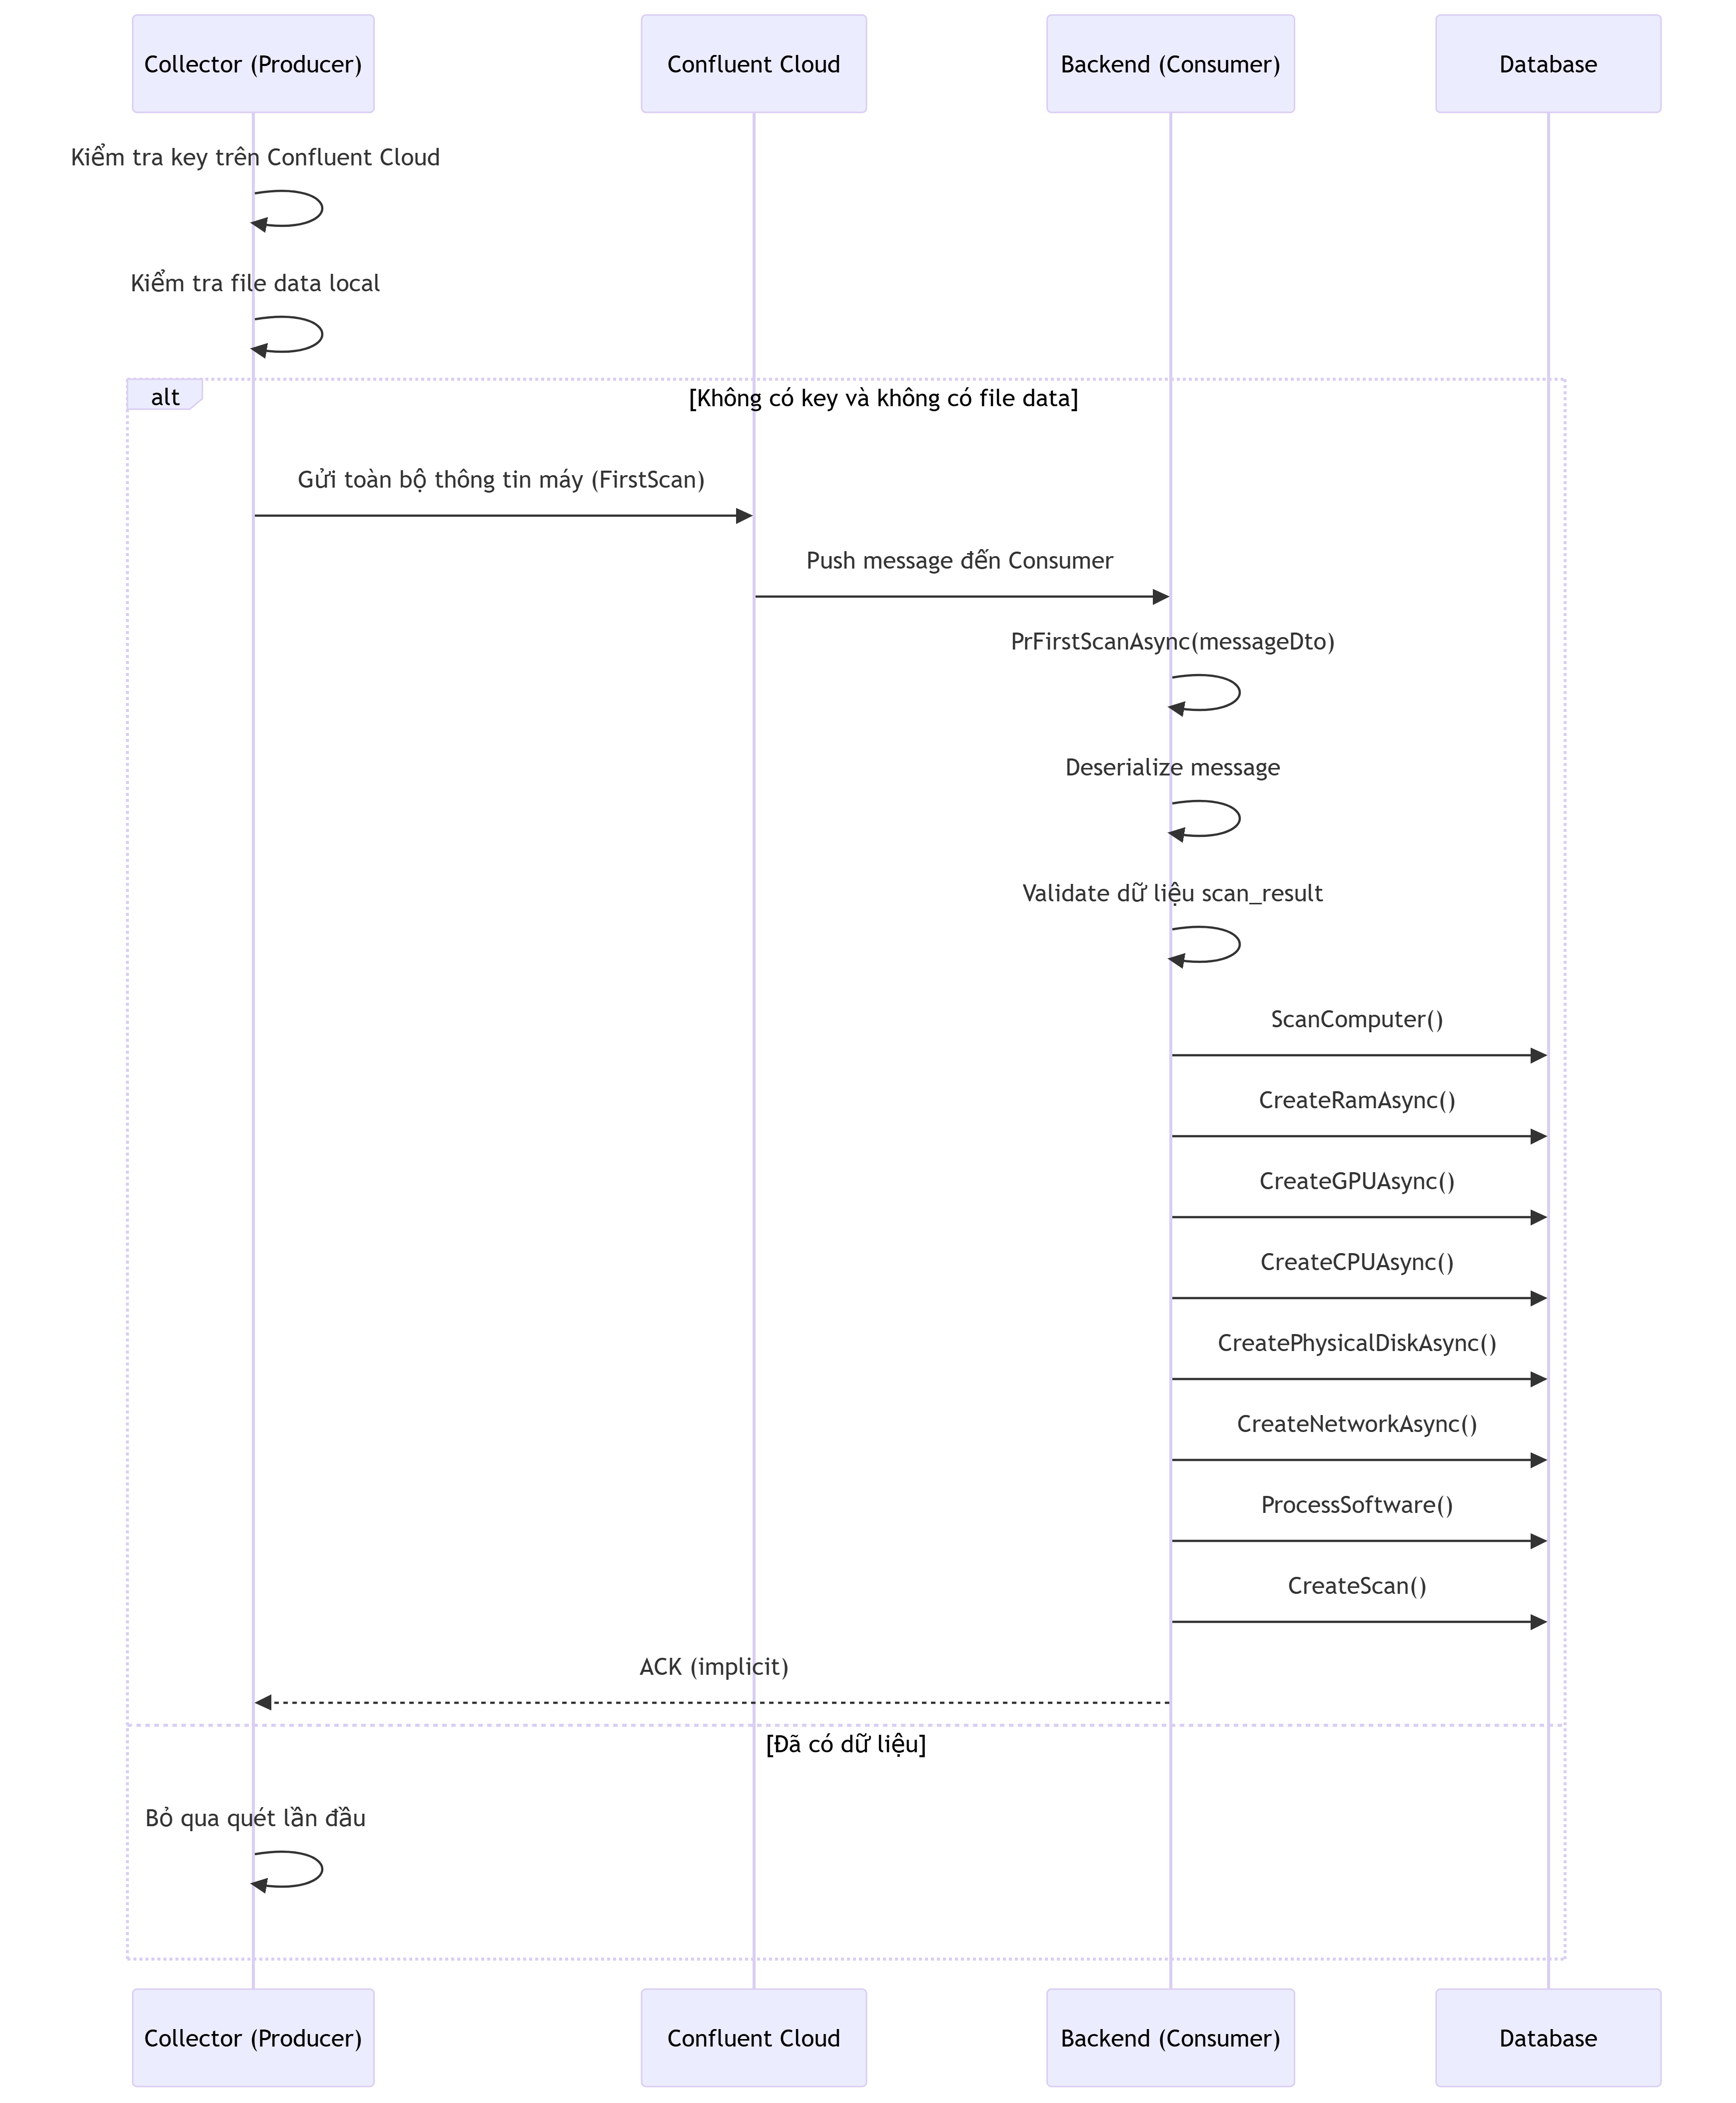
\includegraphics[width=0.8\linewidth]{Images/C6/firstScan.png}
        \vspace{10pt}
        \caption{Sequence Diagram cho quét máy tính lần đầu} 
        \label{fig:enter-label}
    \end{figure}
    \item \textbf{Quét cập nhật thay đổi}
    \begin{figure}[H]
        \centering
        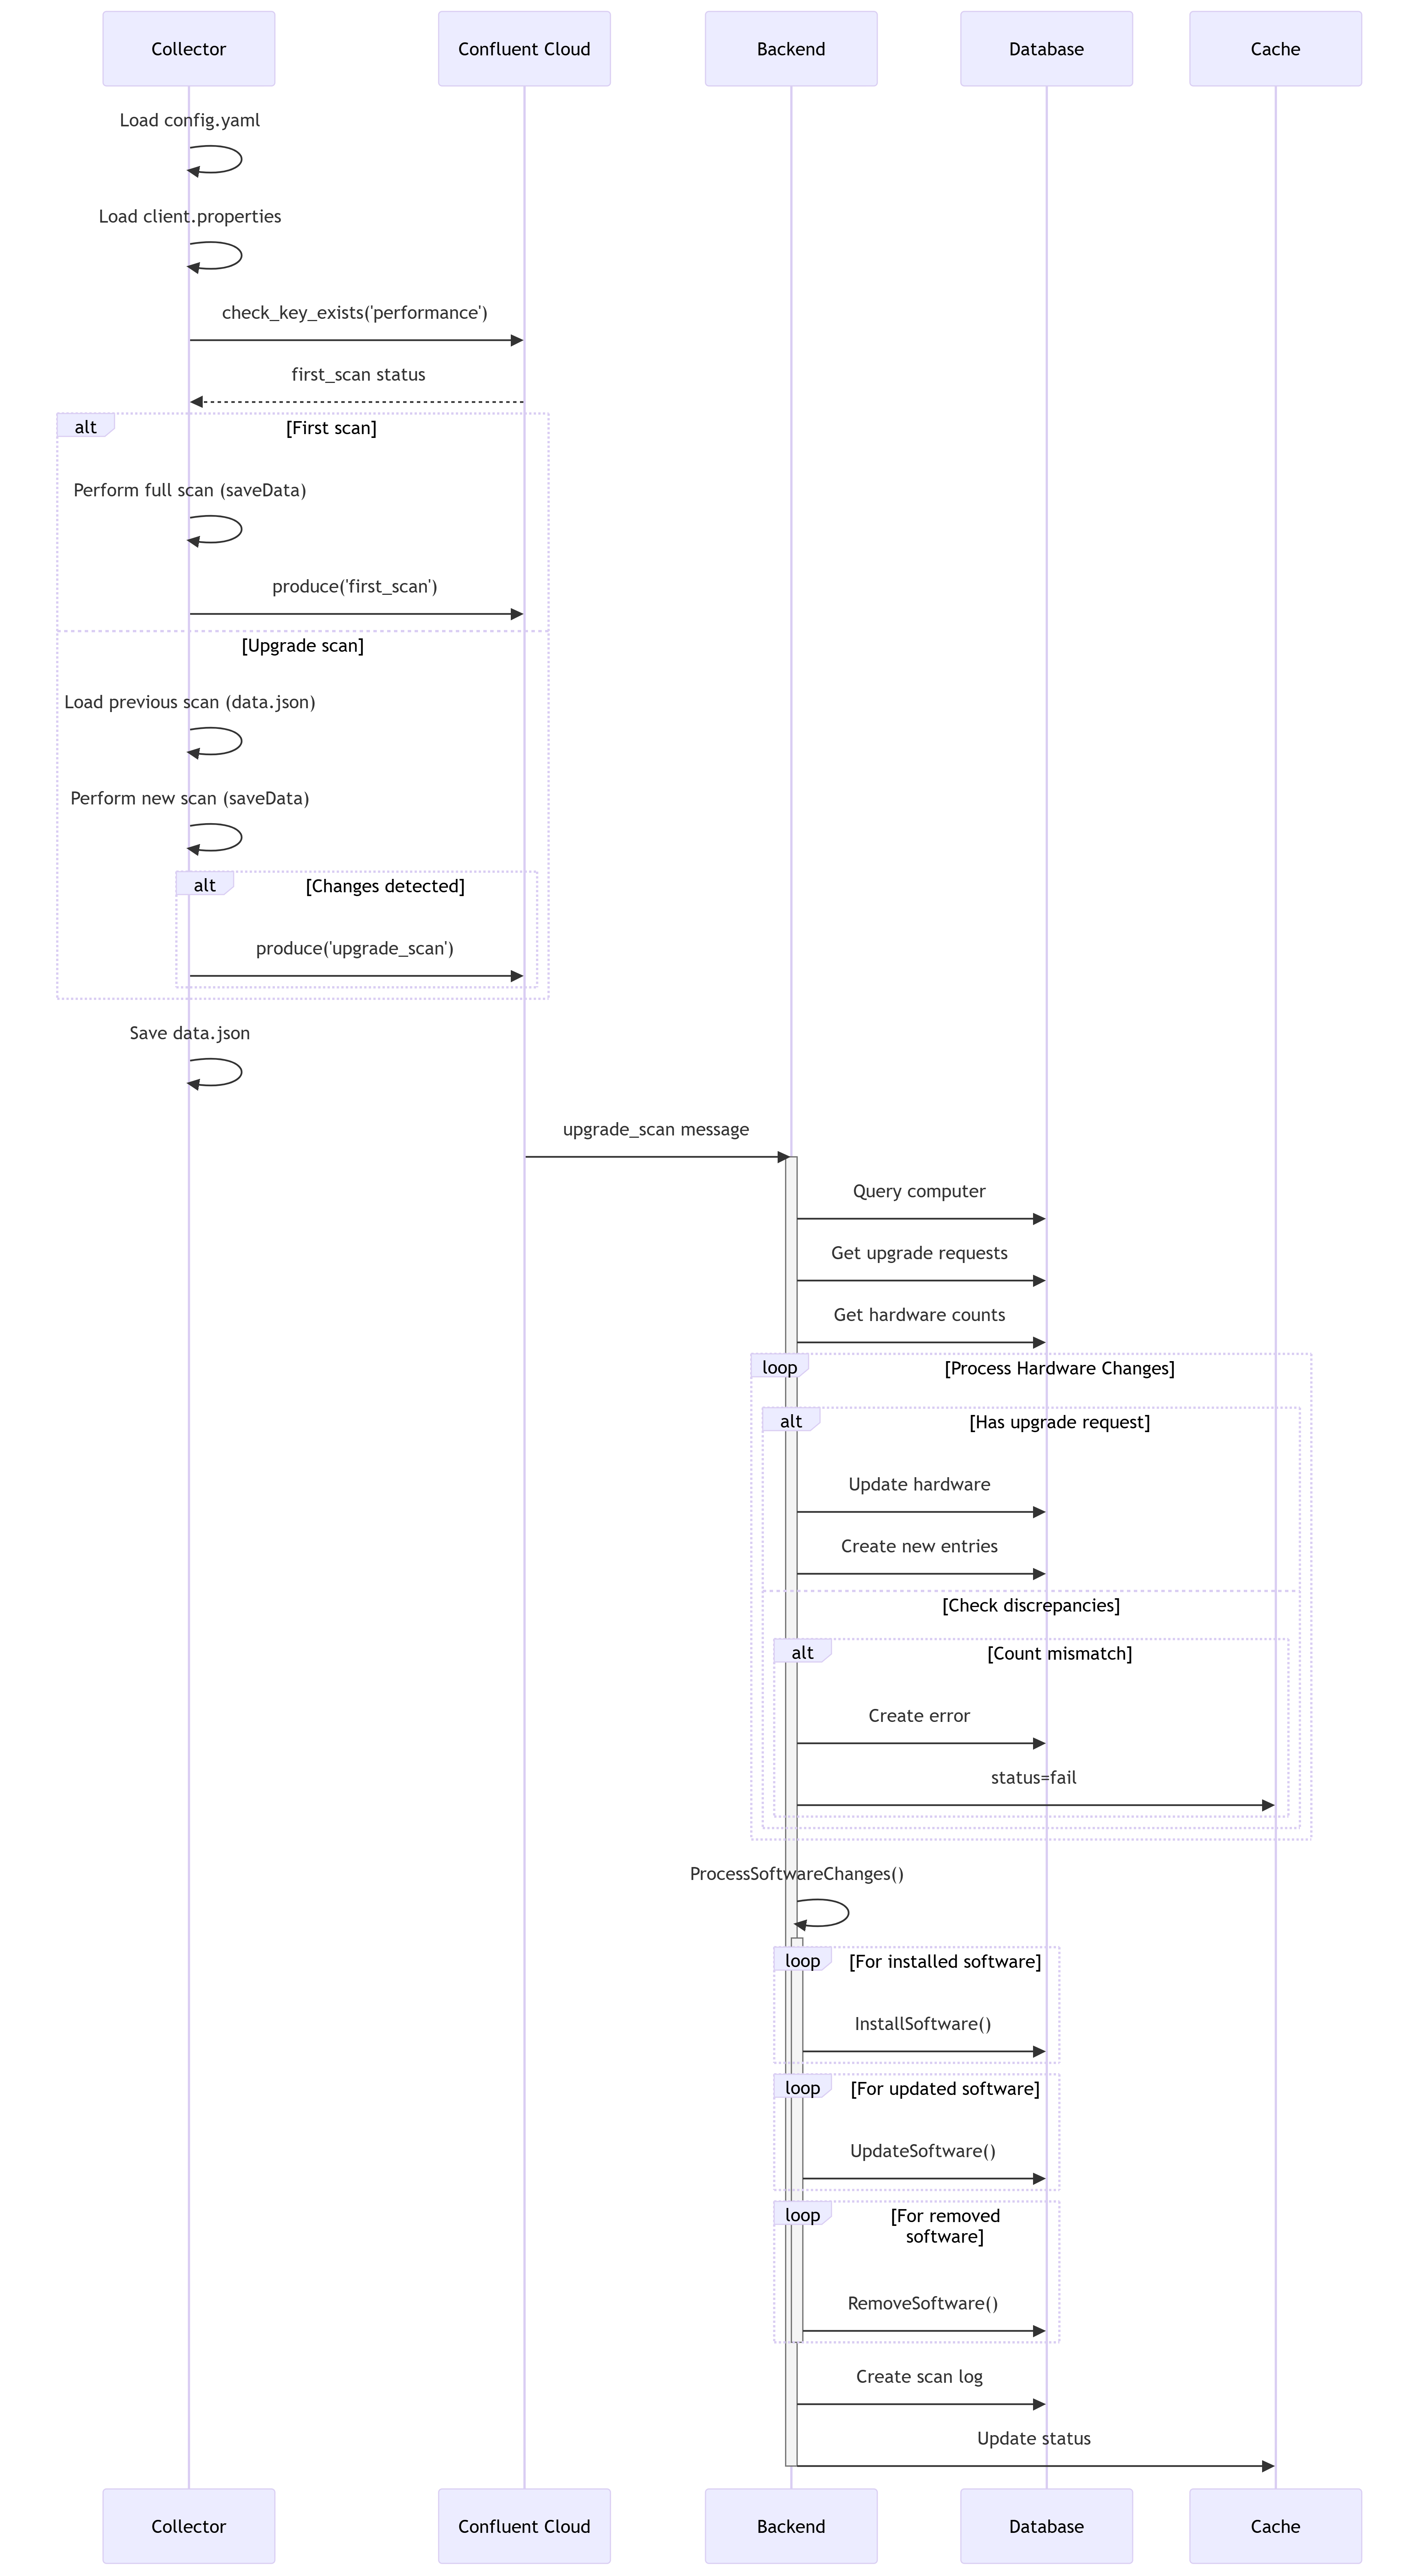
\includegraphics[width=0.8\linewidth]{Images/C6/Sequence-diagrams/upgradeScan.png}
        \vspace{10pt}
        \caption{Sequence Digram cho cập nhật thay đổi}
    \end{figure}
    \item \textbf{Phát hiện lỗi}
    \begin{figure}[H]
        \centering
        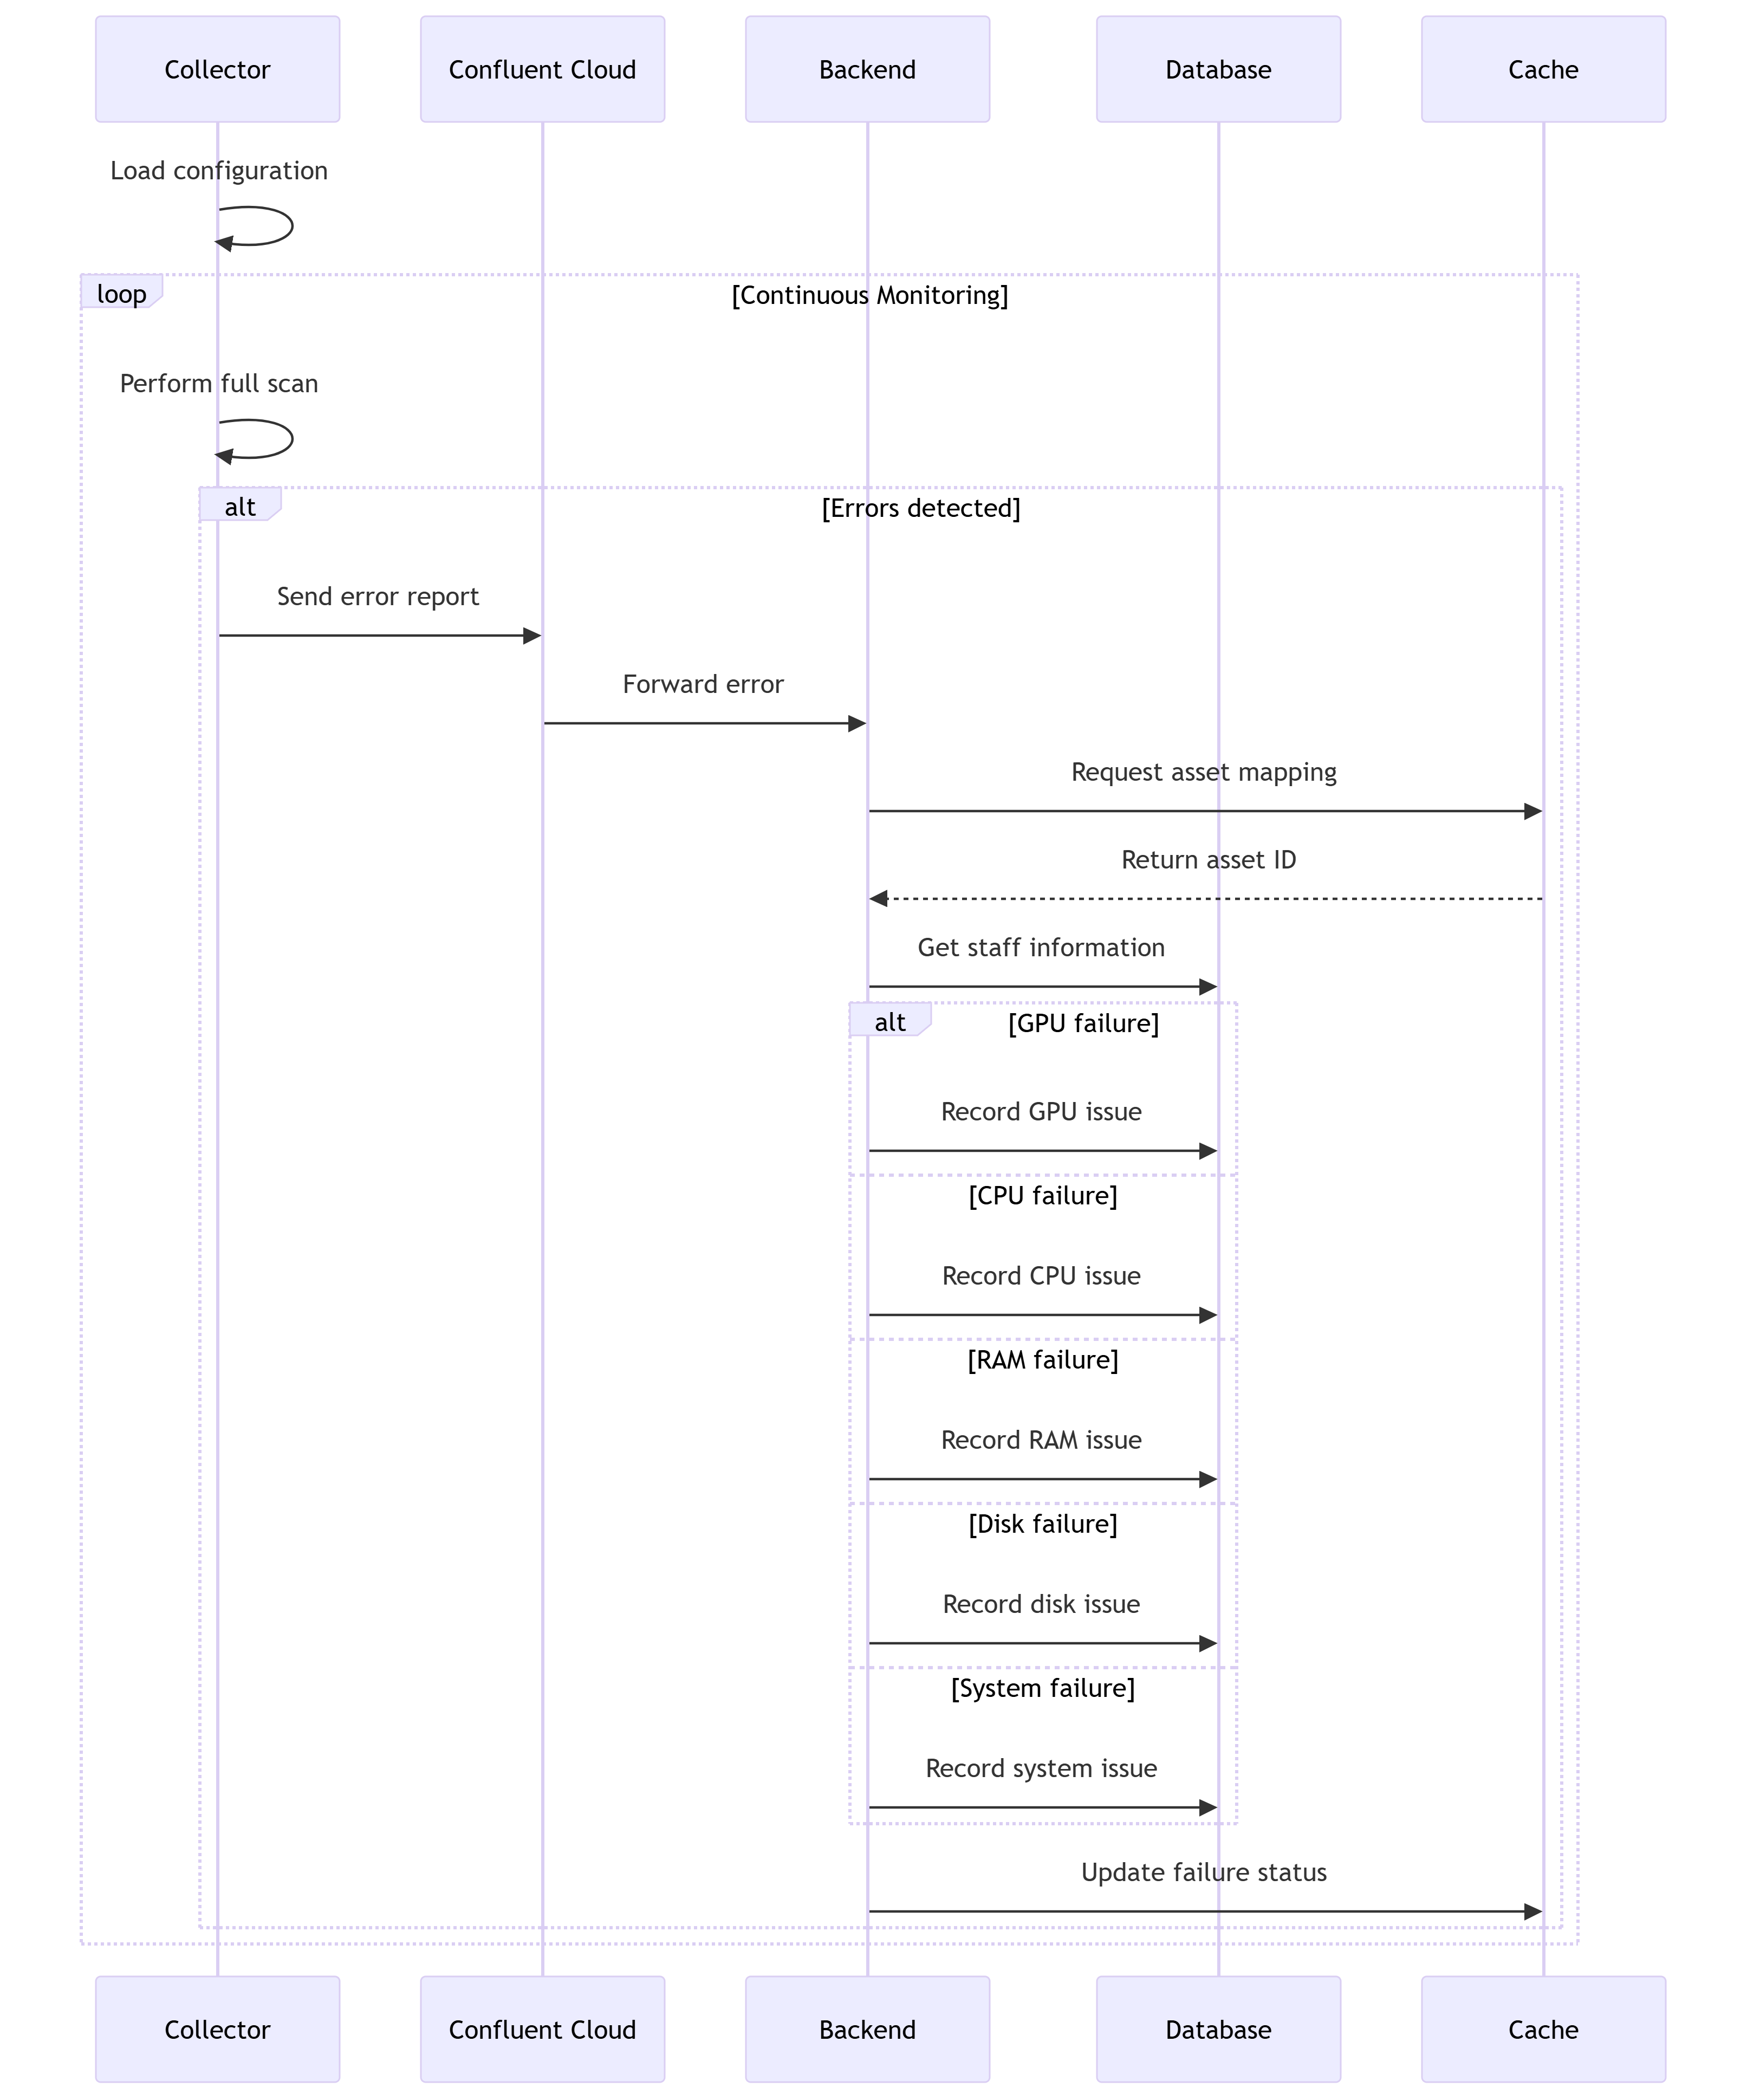
\includegraphics[width=\linewidth]{Images/C6/Sequence-diagrams/errorScan.png}
        \vspace{10pt}
        \caption{Sequence Digram cho phát hiện lỗi}
    \end{figure}
    \item \textbf{Dự đoán hiệu suất tài sản}
    \begin{figure}[H]
        \centering
        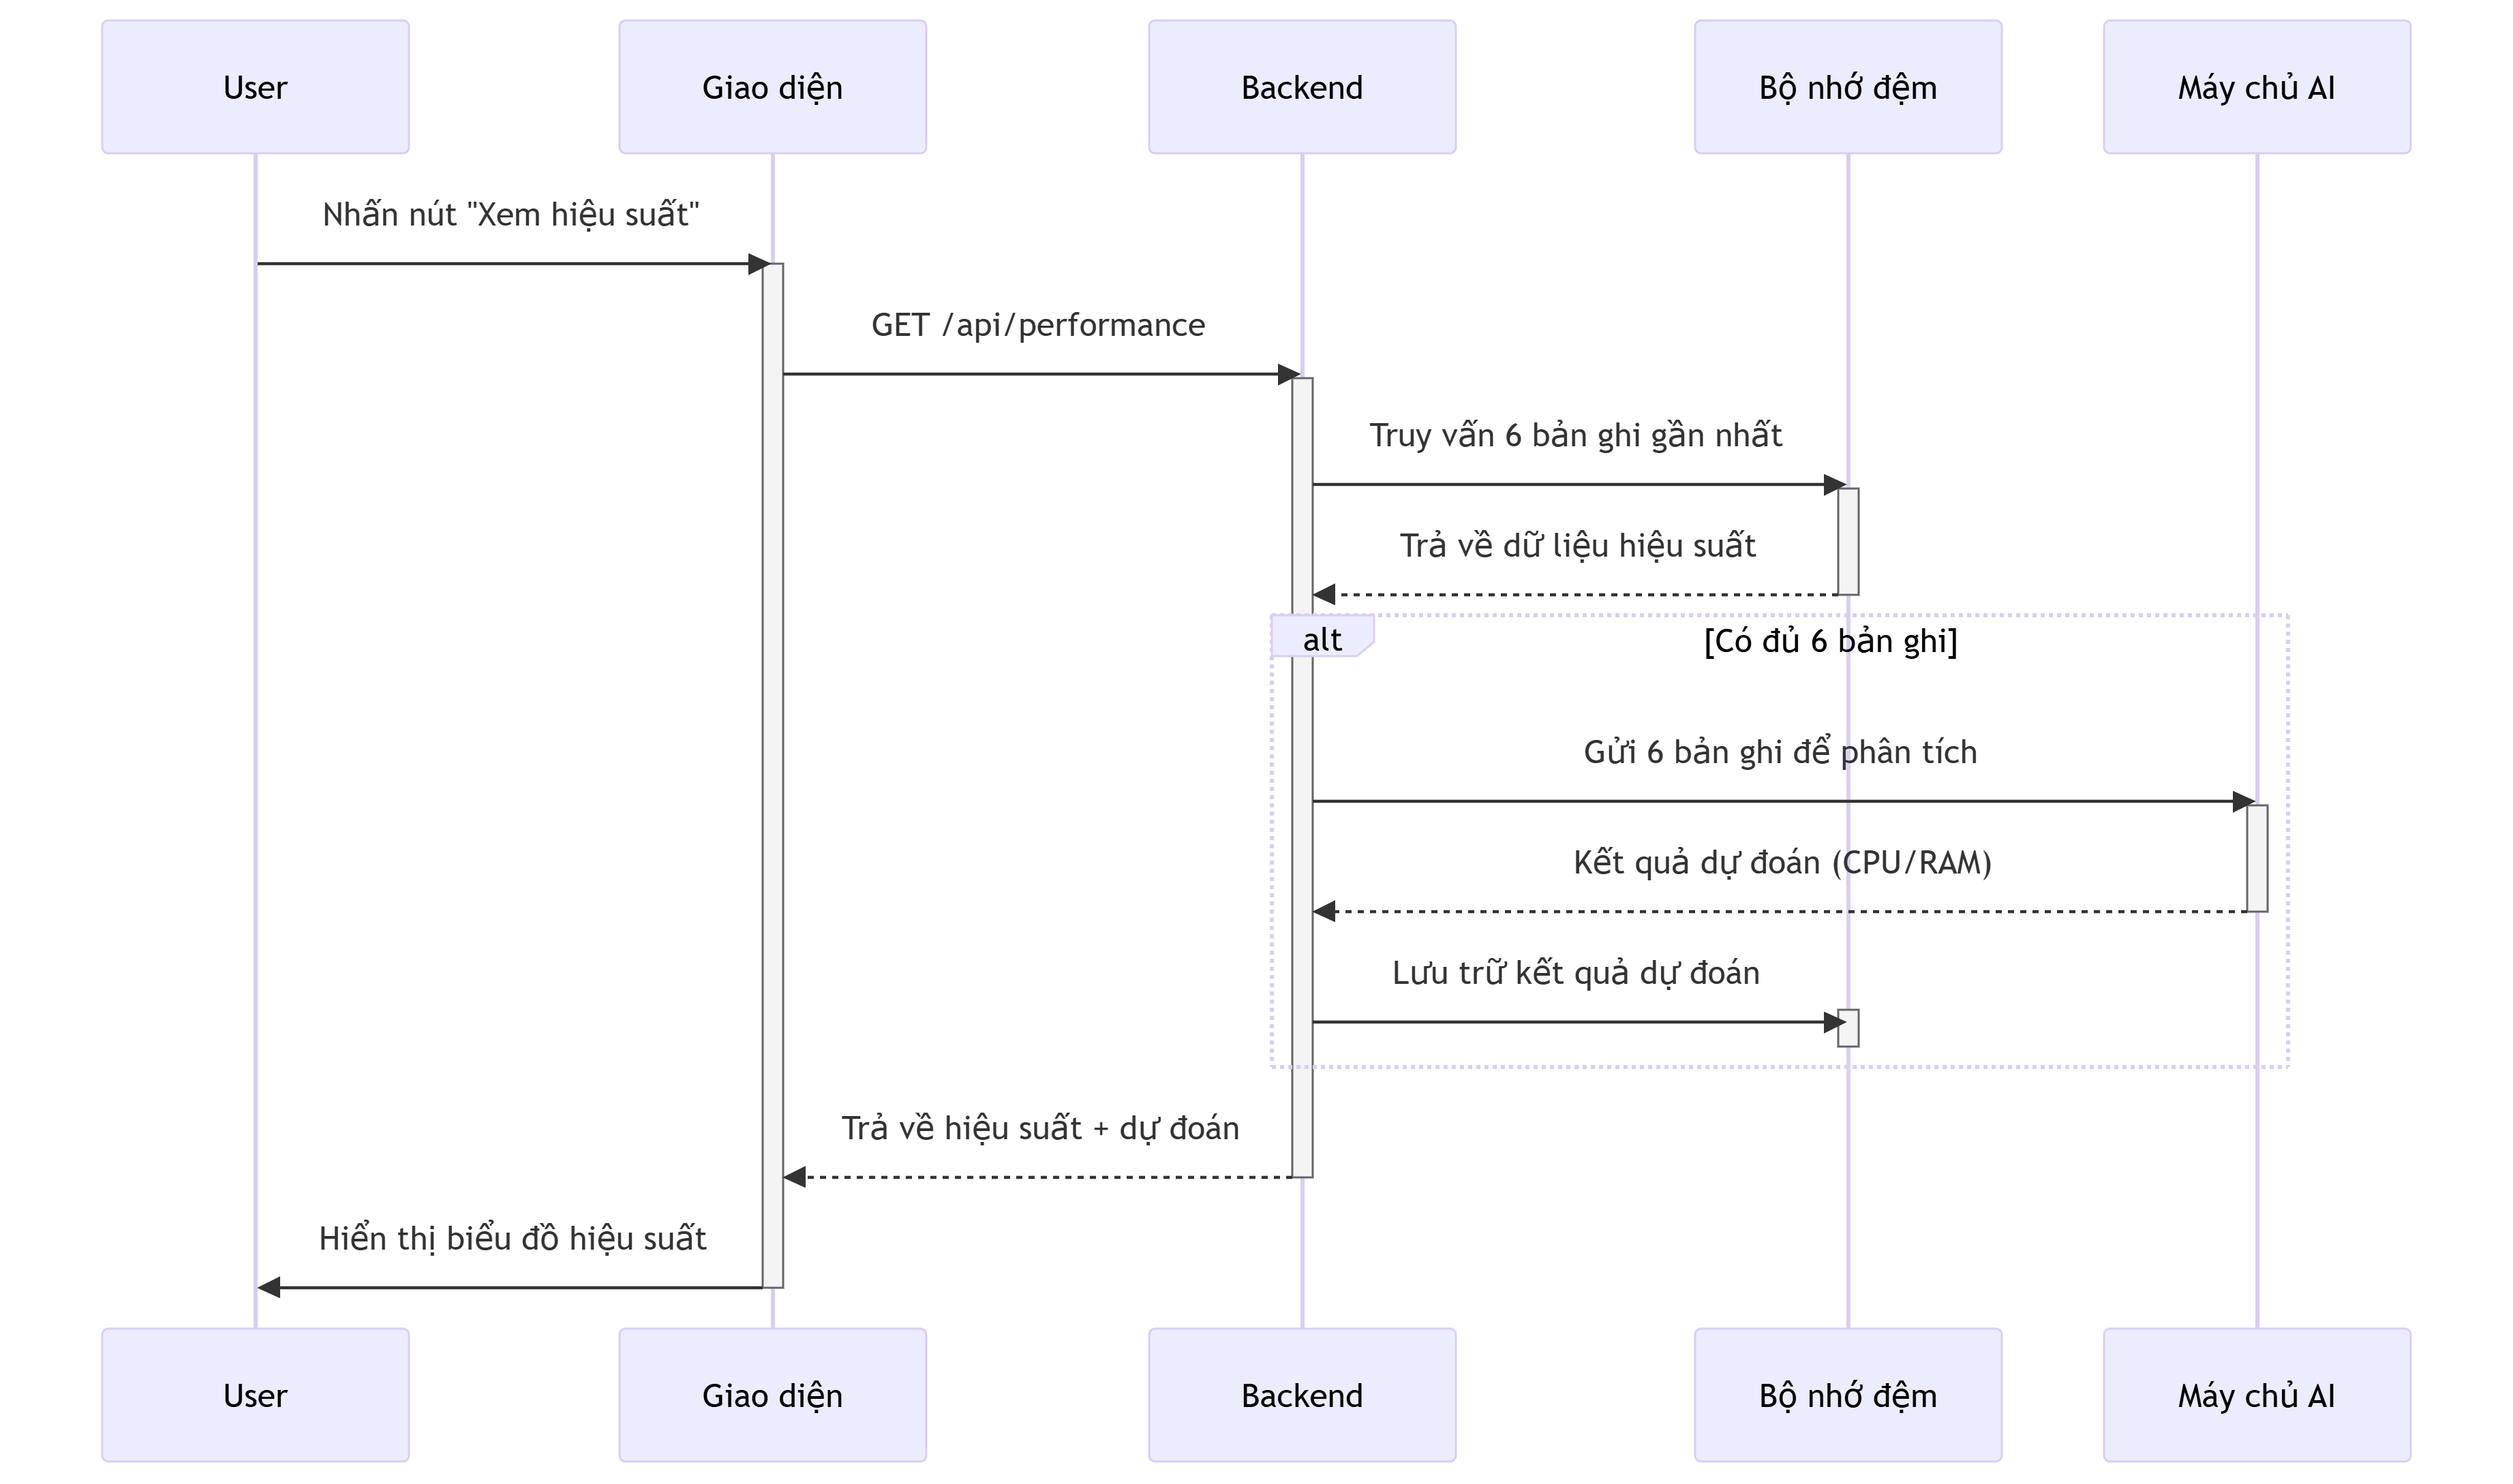
\includegraphics[width=\linewidth]{Images//C6/ai_sequence.png}
        \vspace{10pt}
        \caption{Sequence Diagram cho dự đoán hiệu suất tài sản} 
        \label{fig:enter-label}
    \end{figure}
    \item \textbf{Giám sát máy tính}
    \begin{figure}[H]
        \centering
        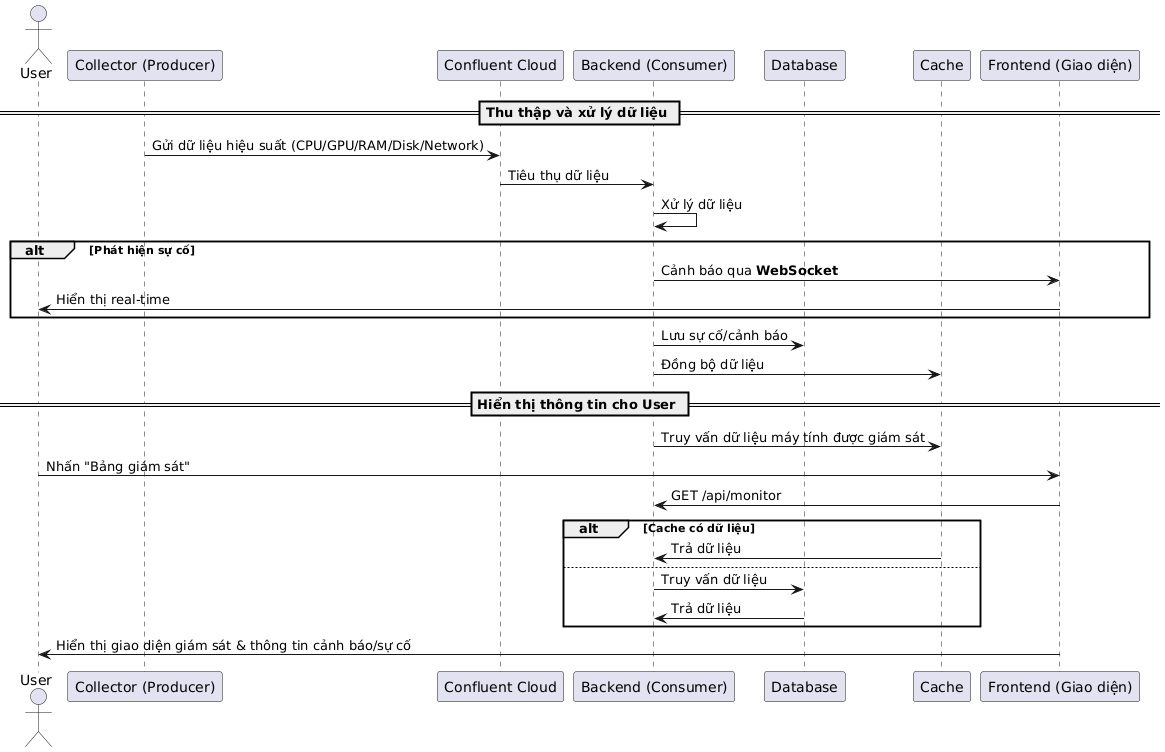
\includegraphics[width=\linewidth]{Images/C6/Sequence-diagrams/sequence-monitor.png}
        \vspace{10pt}
        \caption{Sequence Diagram cho Giám sát máy tính} 
        \label{fig:enter-label}
    \end{figure}
    \item \textbf{Thanh lý tài sản}
    \begin{figure}[H]
        \centering
        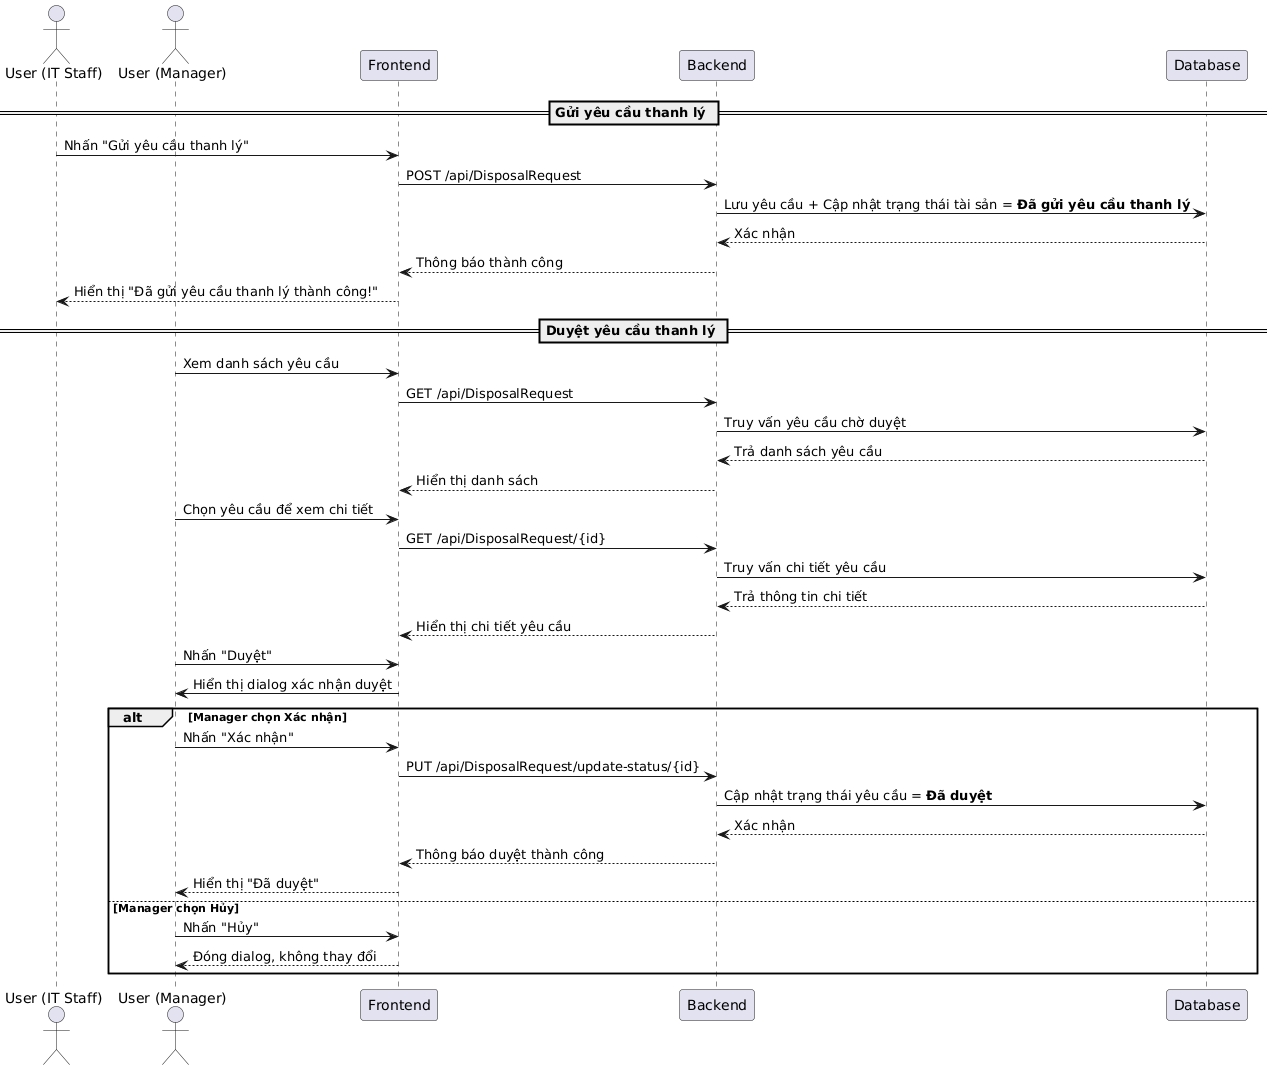
\includegraphics[width=\linewidth]{Images/C6/Sequence-diagrams/sequence-disposal.png}
        \vspace{10pt}
        \caption{Sequence Diagram cho Thanh lý tài sản} 
        \label{fig:enter-label}
    \end{figure}
\end{enumerate}
%%%%%%%%%%%%%%%%%%%%%%%%%%%%%%%%%%%%%%%%%%%%%%
\section{Phụ lục Hiện thực giao diện hệ thống}
\begin{itemize}[label=--]
    \item Hiện thực tính năng Bảng thông tin chung
    \begin{figure}[H]
        \centering
        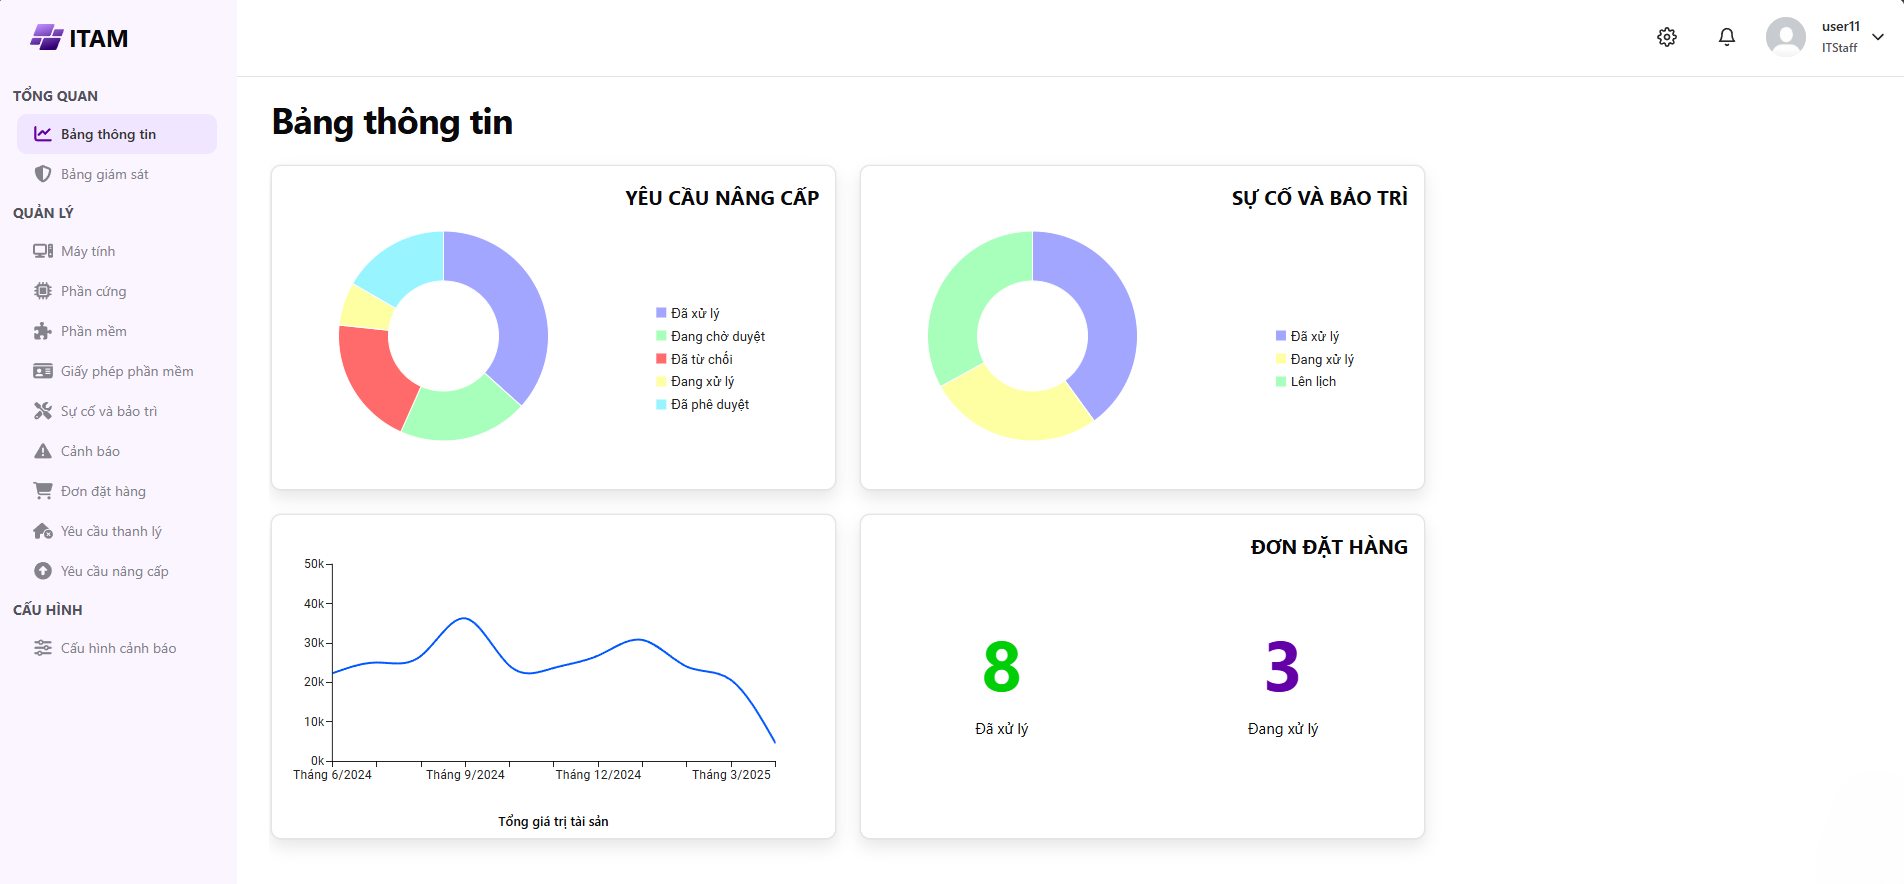
\includegraphics[width=14cm]{Images/C6/UI-Hienthuc/bangthongtin1.png}
        \vspace{15pt}
        \caption{Giao diện hiện thực tính năng Bảng thông tin chung}
    \end{figure}
    
    \item Hiện thực tính năng Giám sát máy tính
    \begin{figure}[H]
        \centering
        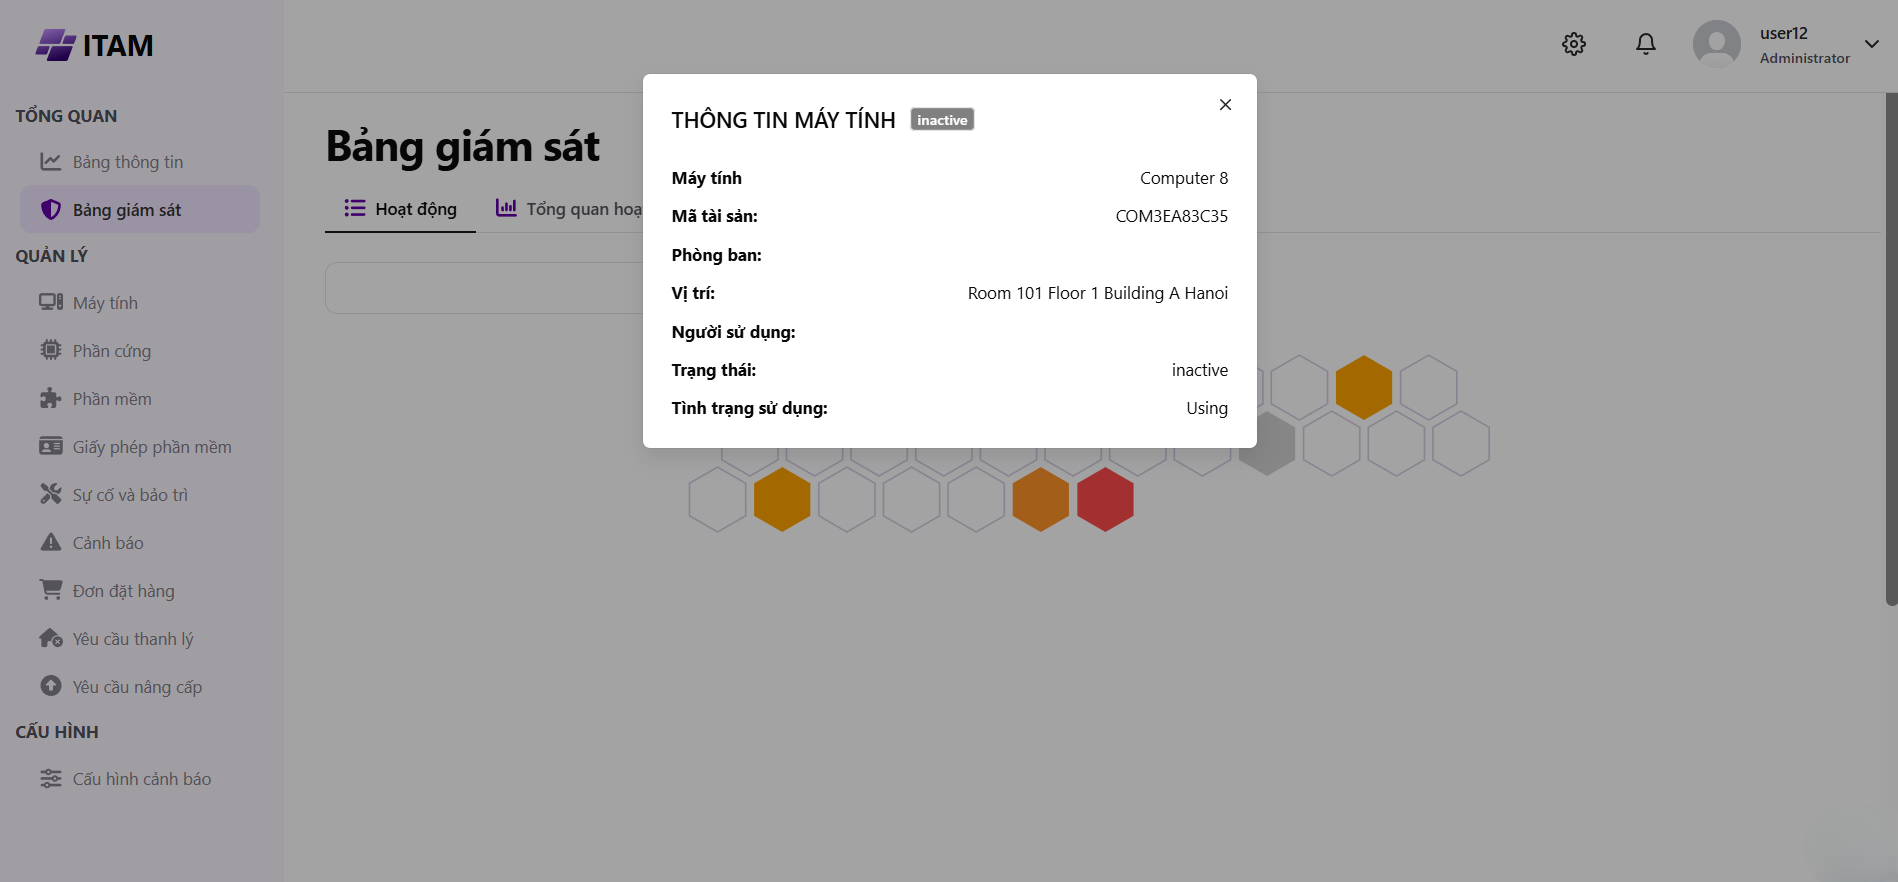
\includegraphics[width=14cm]{Images/C6/UI-Hienthuc/giamsat2.png}
        \vspace{15pt}
        \caption{Giao diện hiện thực tính năng Giám sát - thông tin máy tính}
    \end{figure}

    \item Hiện thực tính năng Quản lý máy tính
    \begin{figure}[H]
        \centering
        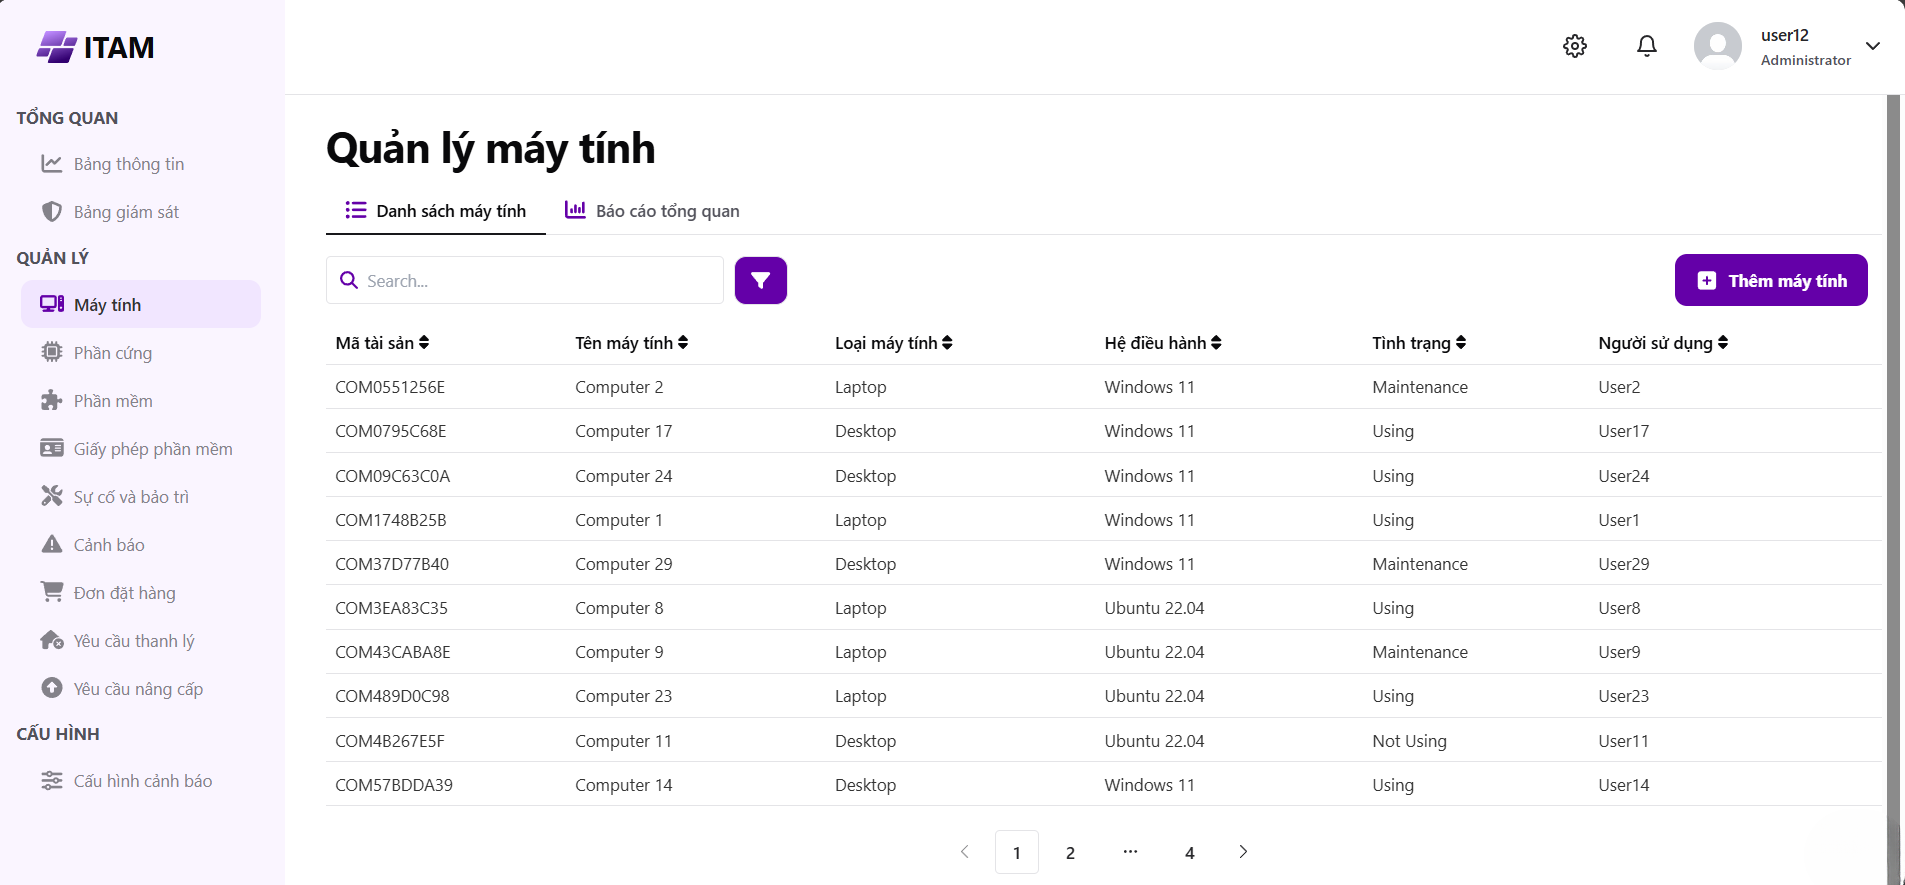
\includegraphics[width=14cm]{Images/C6/UI-Hienthuc/quanlymt0.png}
        \vspace{15pt}
        \caption{Giao diện hiện thực tính năng Quản lý máy tính - danh sách máy tính}
    \end{figure}
    \begin{figure}[H]
        \centering
        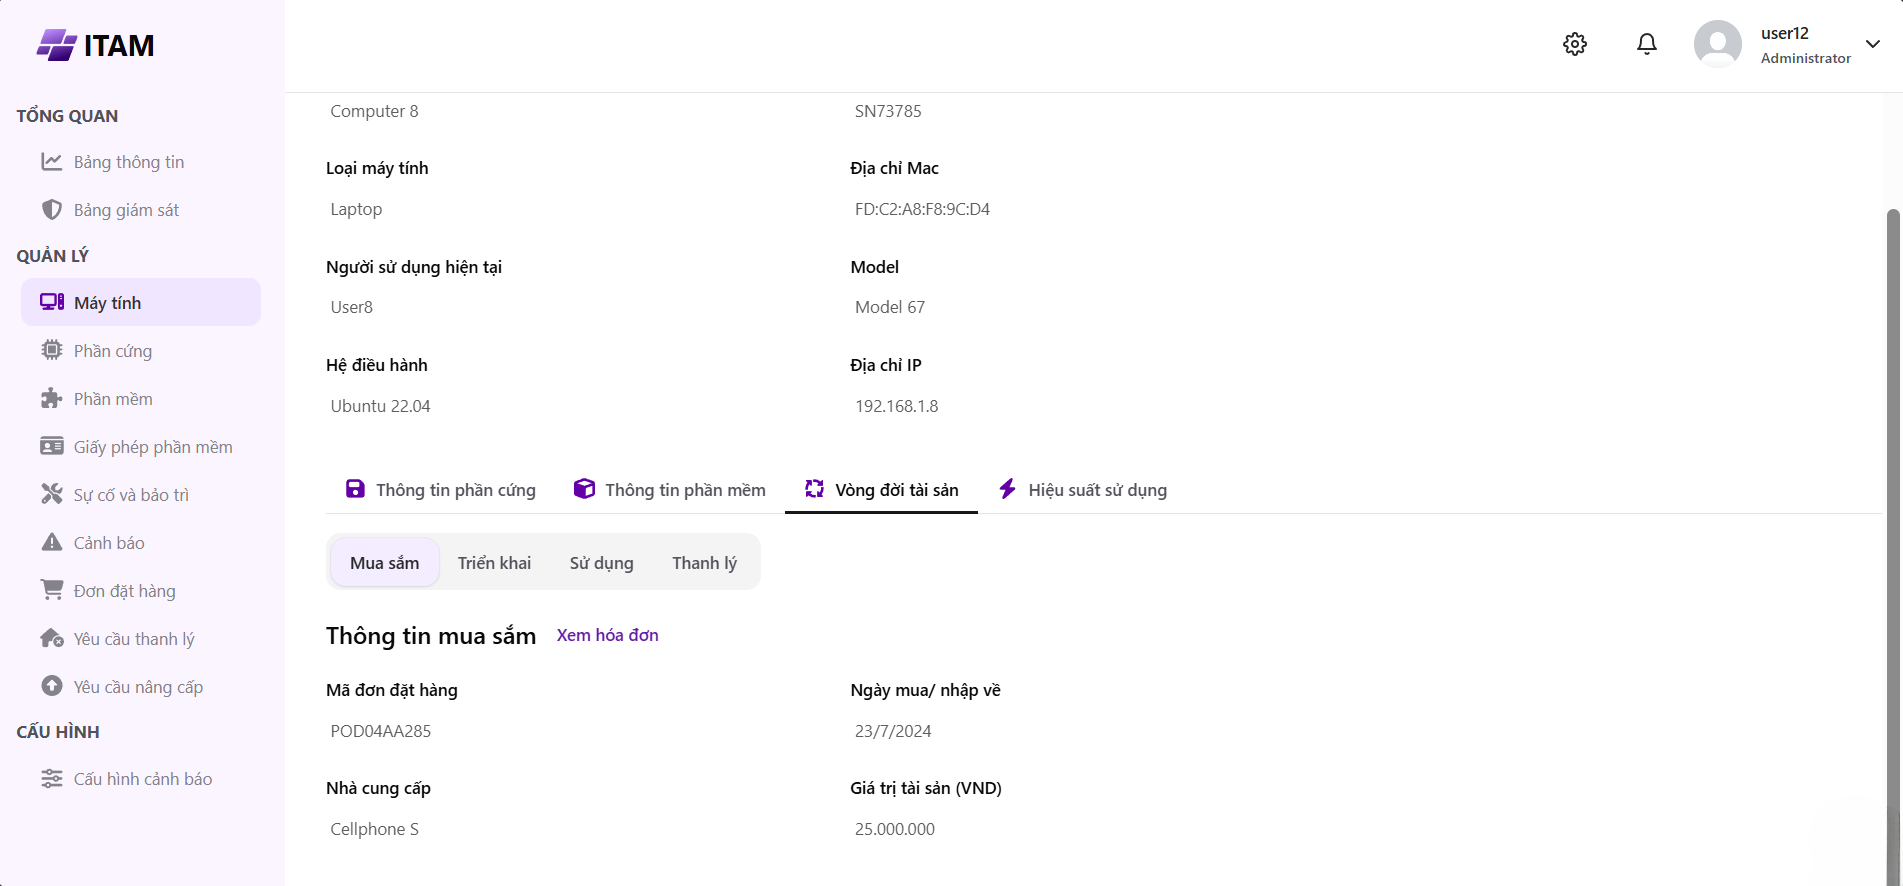
\includegraphics[width=14cm]{Images/C6/UI-Hienthuc/quanlymt2.png}
        \vspace{15pt}
        \caption{Giao diện hiện thực tính năng Quản lý máy tính - vòng đời}
    \end{figure}
    \begin{figure}[H]
        \centering
        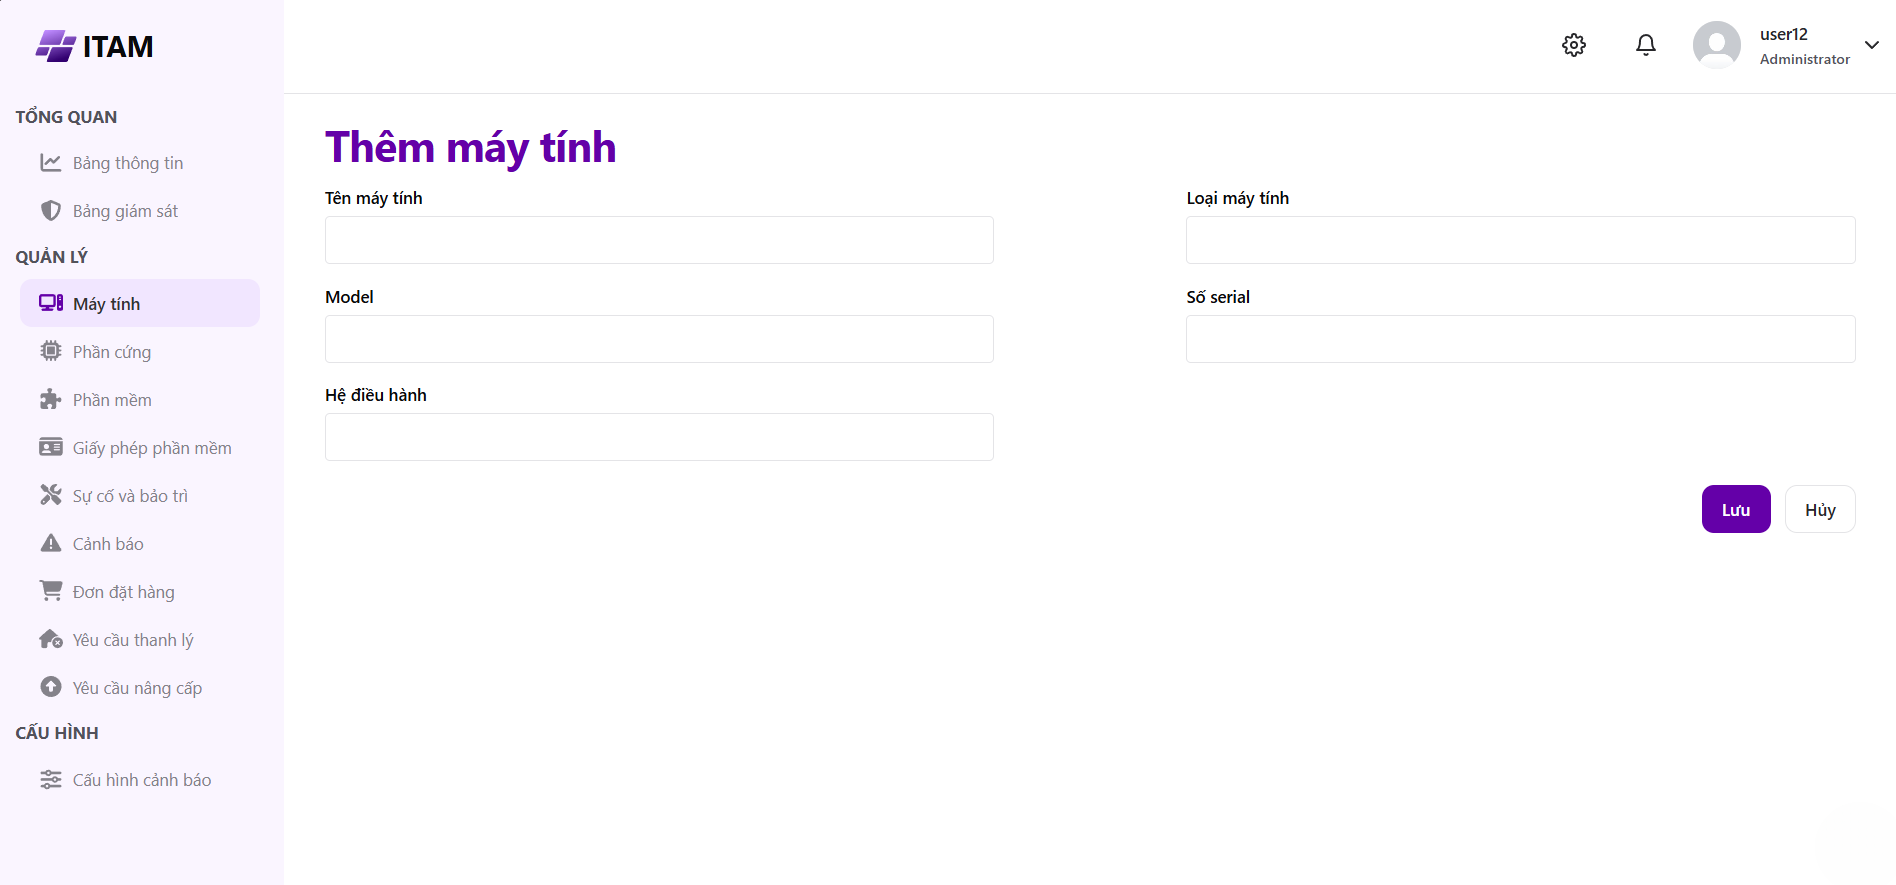
\includegraphics[width=14cm]{Images/C6/UI-Hienthuc/quanlymt4.png}
        \vspace{15pt}
        \caption{Giao diện hiện thực tính năng Quản lý máy tính - thêm máy tính}
    \end{figure}

    \item Hiện thực tính năng Quản lý phần cứng, phần mềm
    \begin{figure}[H]
        \centering
        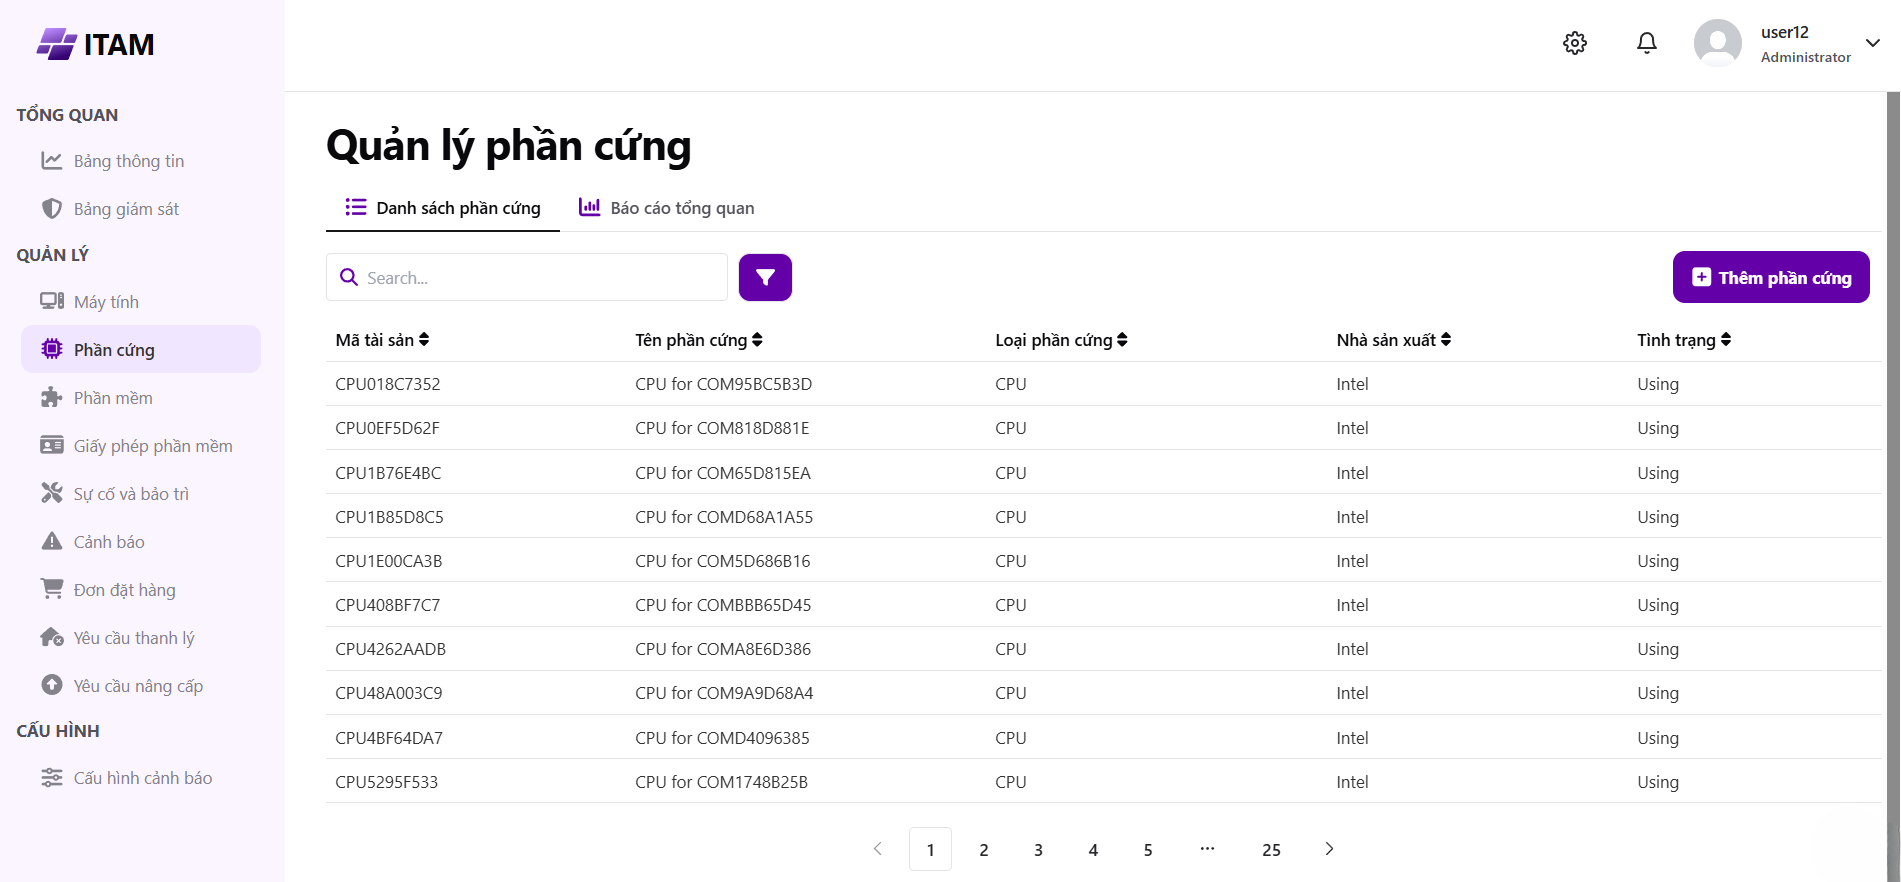
\includegraphics[width=14cm]{Images/C6/UI-Hienthuc/phancung1.png}
        \vspace{15pt}
        \caption{Giao diện hiện thực tính năng Quản lý phần cứng - danh sách}
    \end{figure}
    \begin{figure}[H]
        \centering
        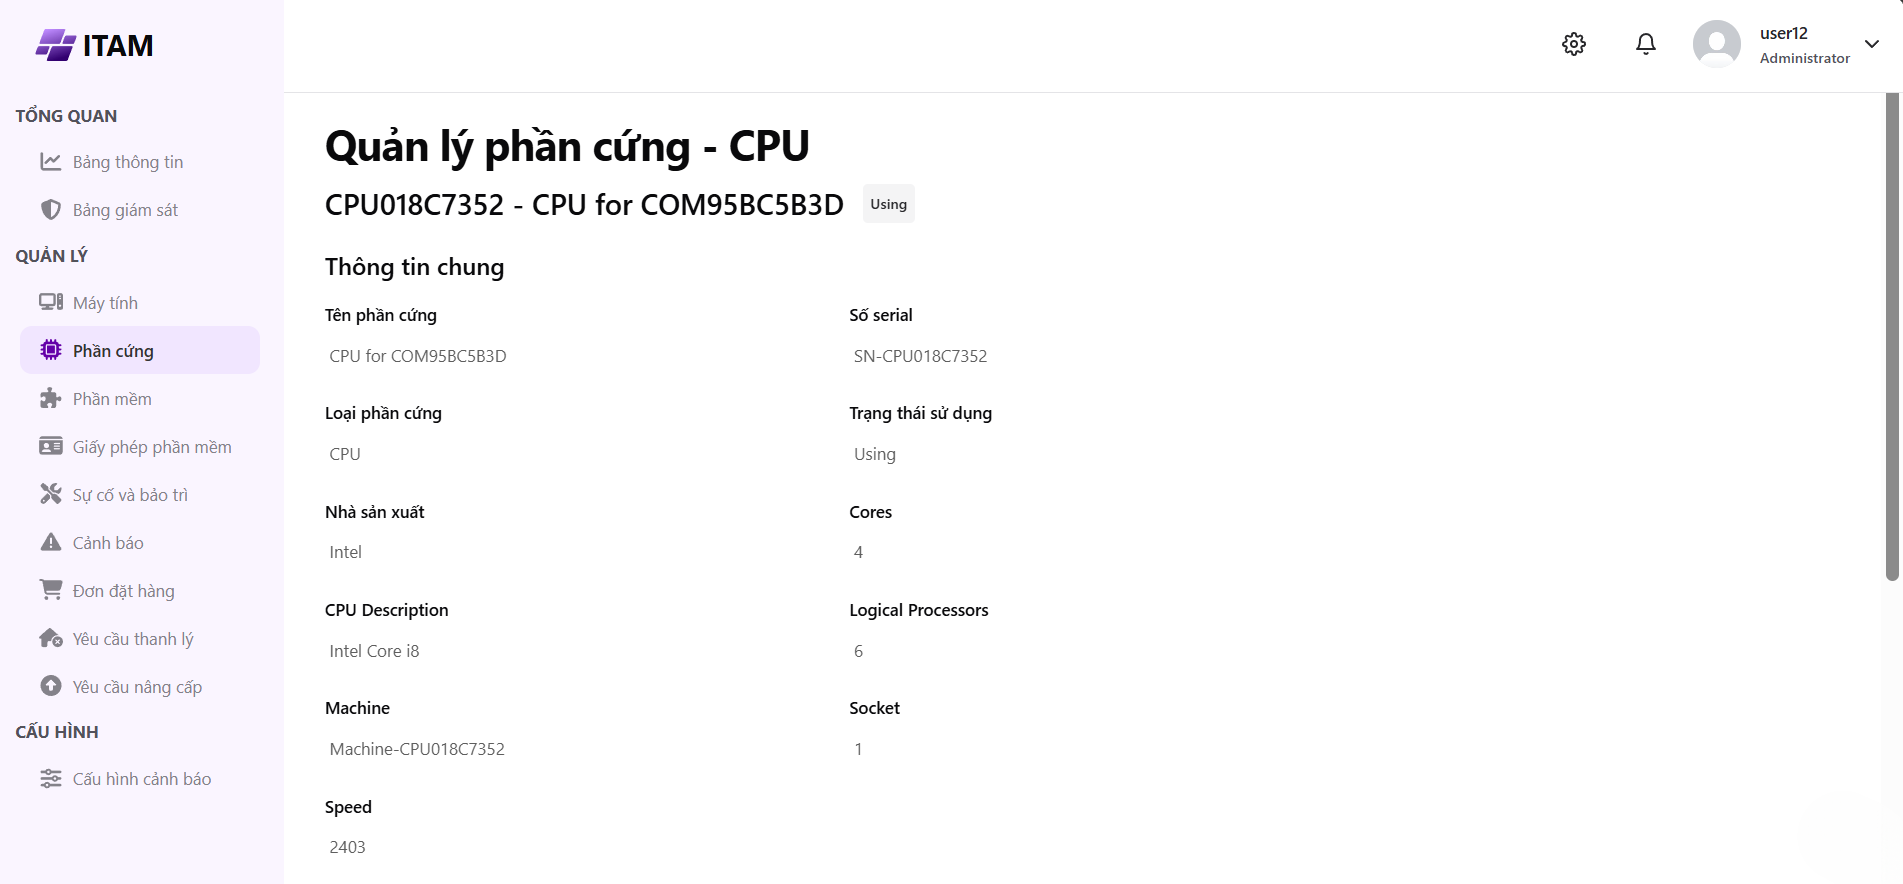
\includegraphics[width=14cm]{Images/C6/UI-Hienthuc/phancung2.png}
        \vspace{15pt}
        \caption{Giao diện hiện thực tính năng Quản lý phần cứng - chi tiết}
    \end{figure}
    \begin{figure}[H]
        \centering
        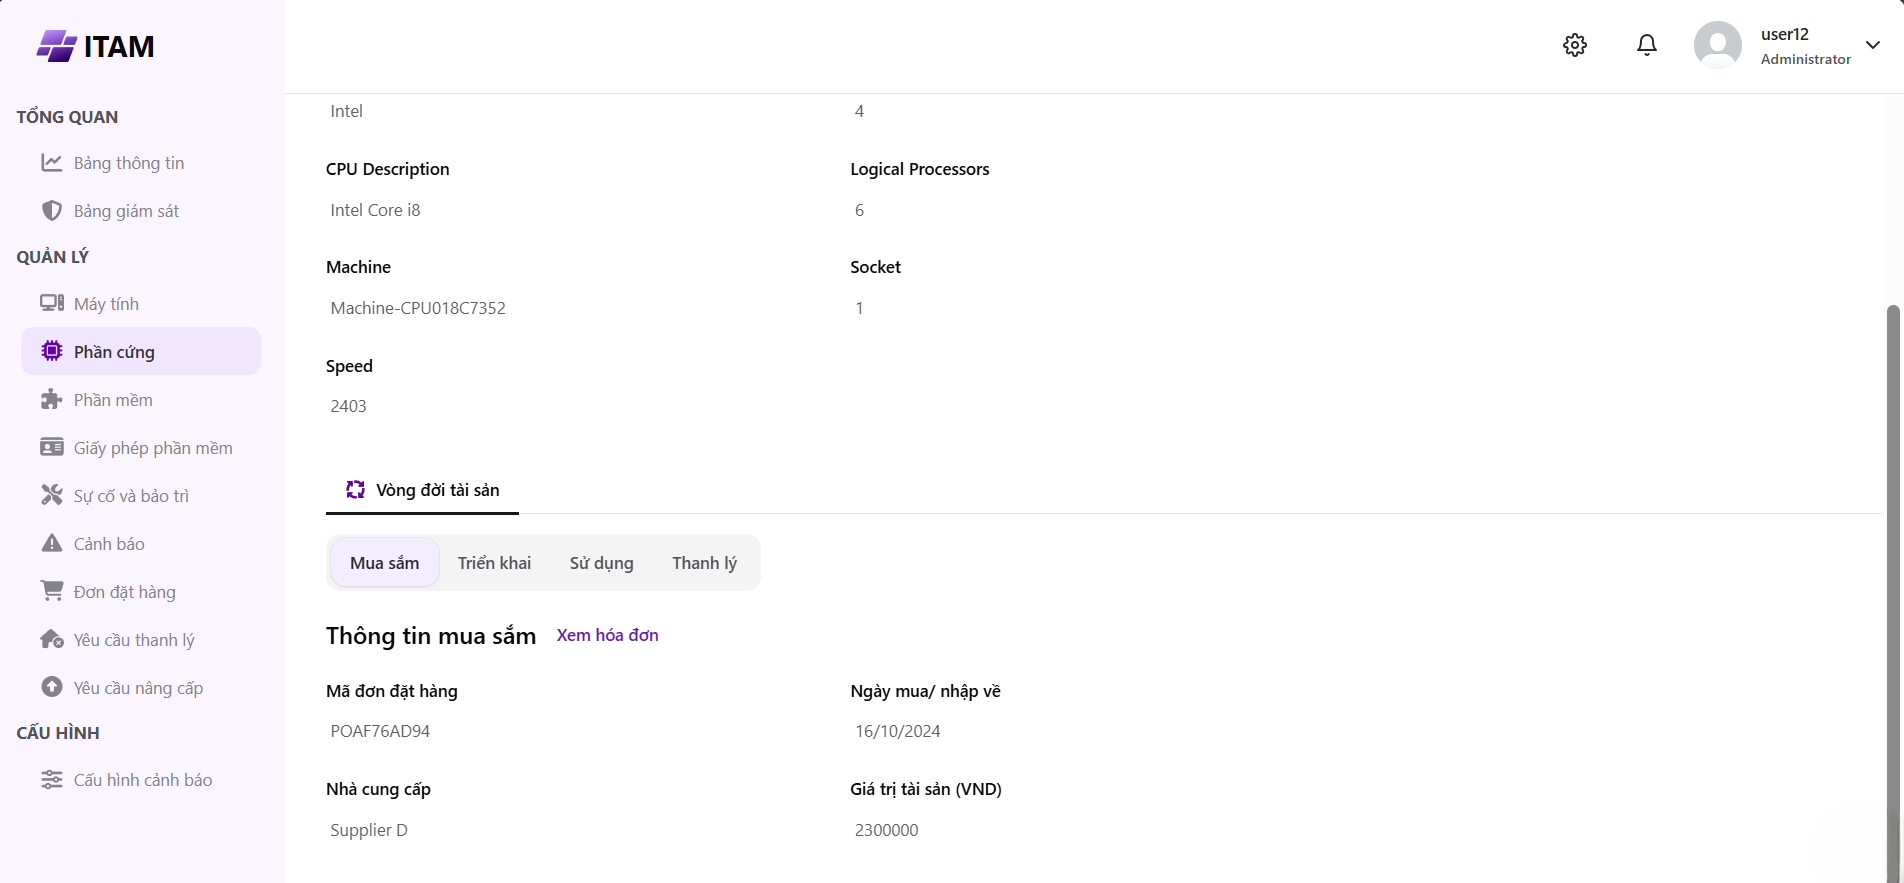
\includegraphics[width=14cm]{Images/C6/UI-Hienthuc/phancung3.png}
        \vspace{15pt}
        \caption{Giao diện hiện thực tính năng Quản lý phần cứng - vòng đời}
    \end{figure}
    \begin{figure}[H]
        \centering
        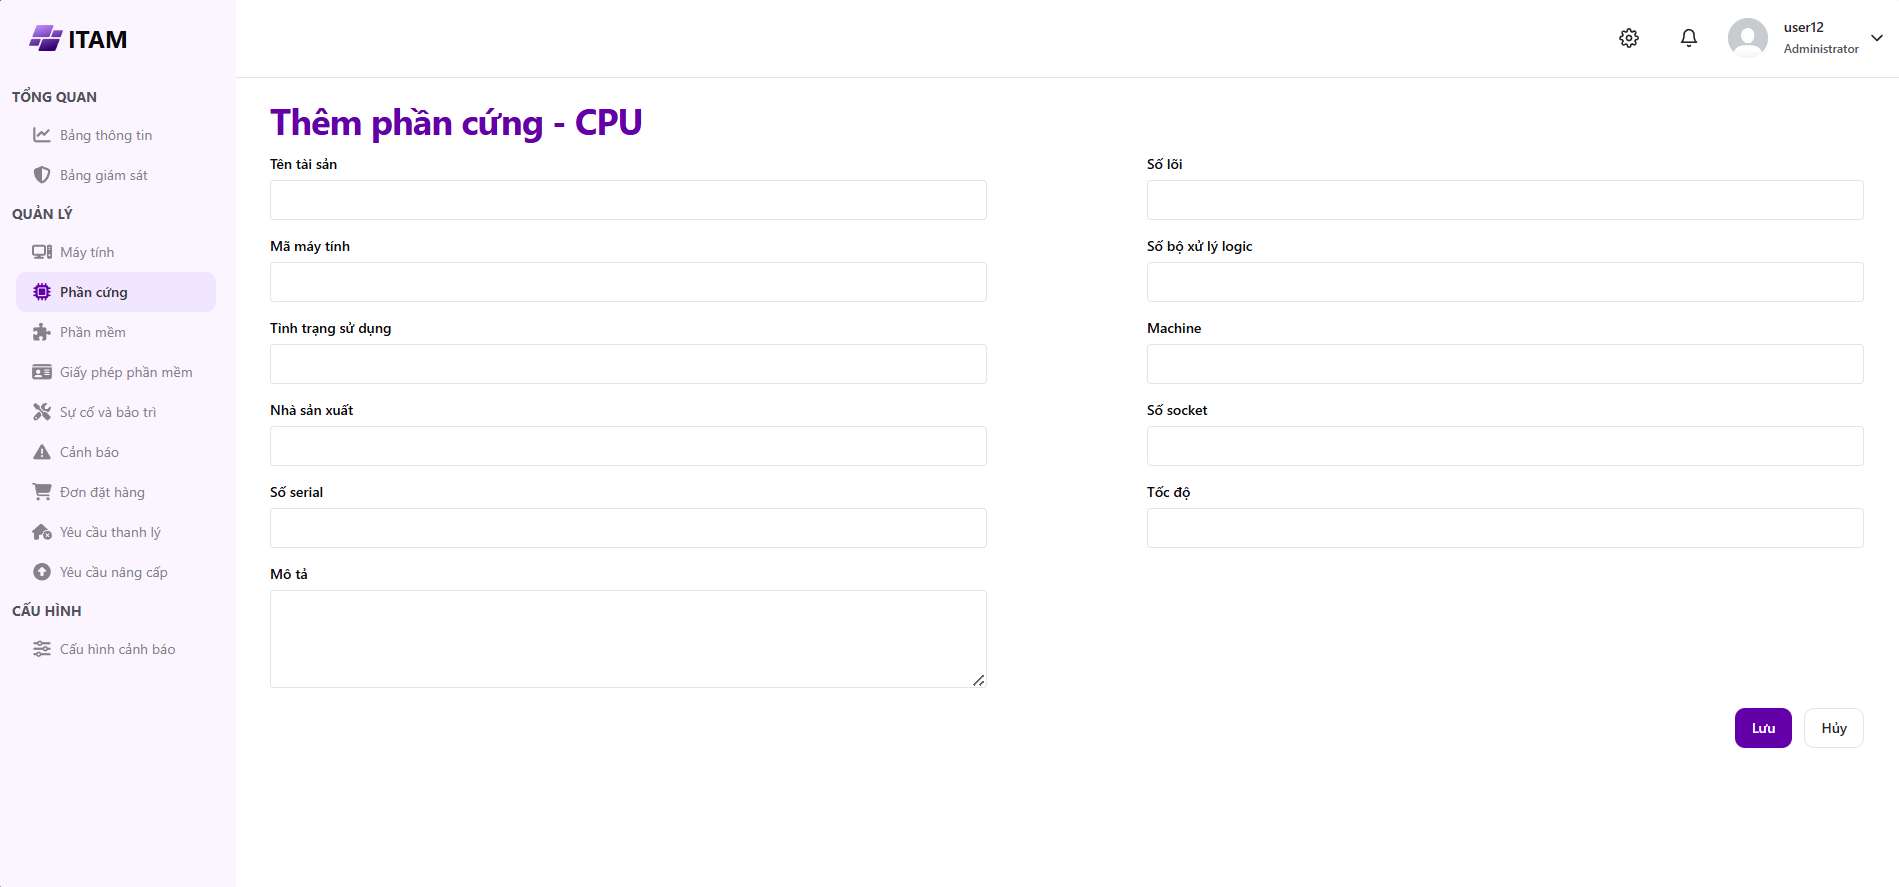
\includegraphics[width=14cm]{Images/C6/UI-Hienthuc/phancung4.png}
        \vspace{15pt}
        \caption{Giao diện hiện thực tính năng Quản lý phần cứng - thêm phần cứng}
    \end{figure}
    \begin{figure}[H]
        \centering
        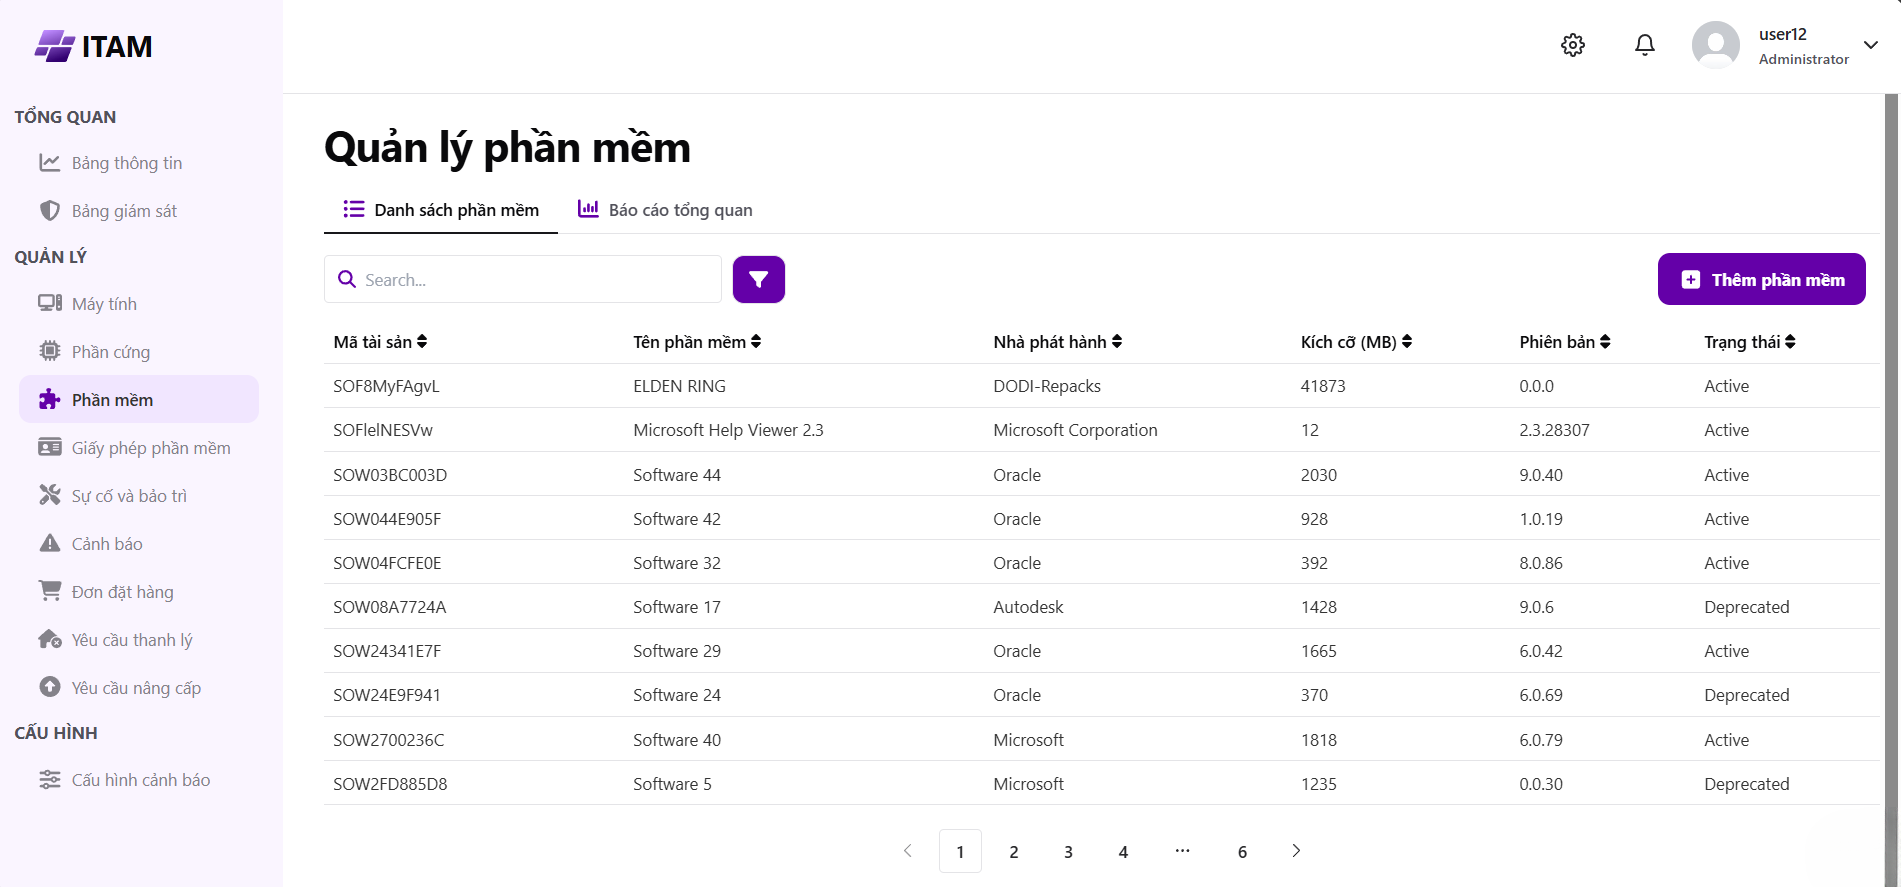
\includegraphics[width=14cm]{Images/C6/UI-Hienthuc/phanmem1.png}
        \vspace{15pt}
        \caption{Giao diện hiện thực tính năng Quản lý phần mềm - danh sách}
    \end{figure}
    \begin{figure}[H]
        \centering
        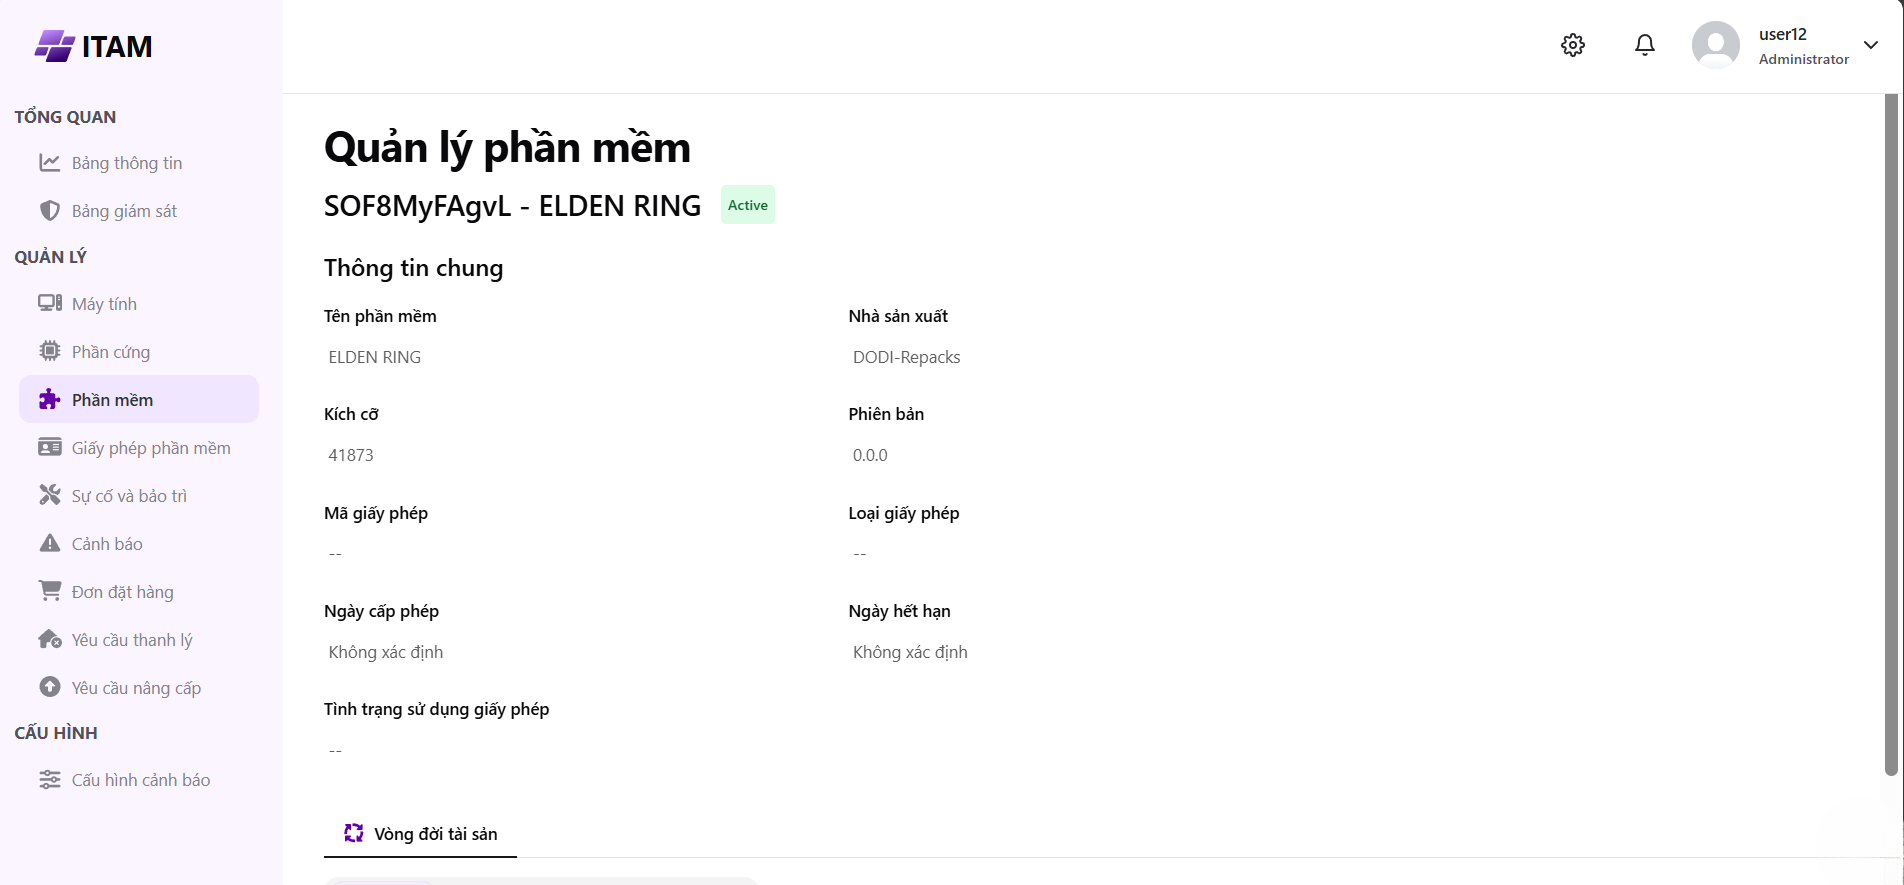
\includegraphics[width=14cm]{Images/C6/UI-Hienthuc/phanmem2.png}
        \vspace{15pt}
        \caption{Giao diện hiện thực tính năng Quản lý phần mềm - chi tiết}
    \end{figure}
    \begin{figure}[H]
        \centering
        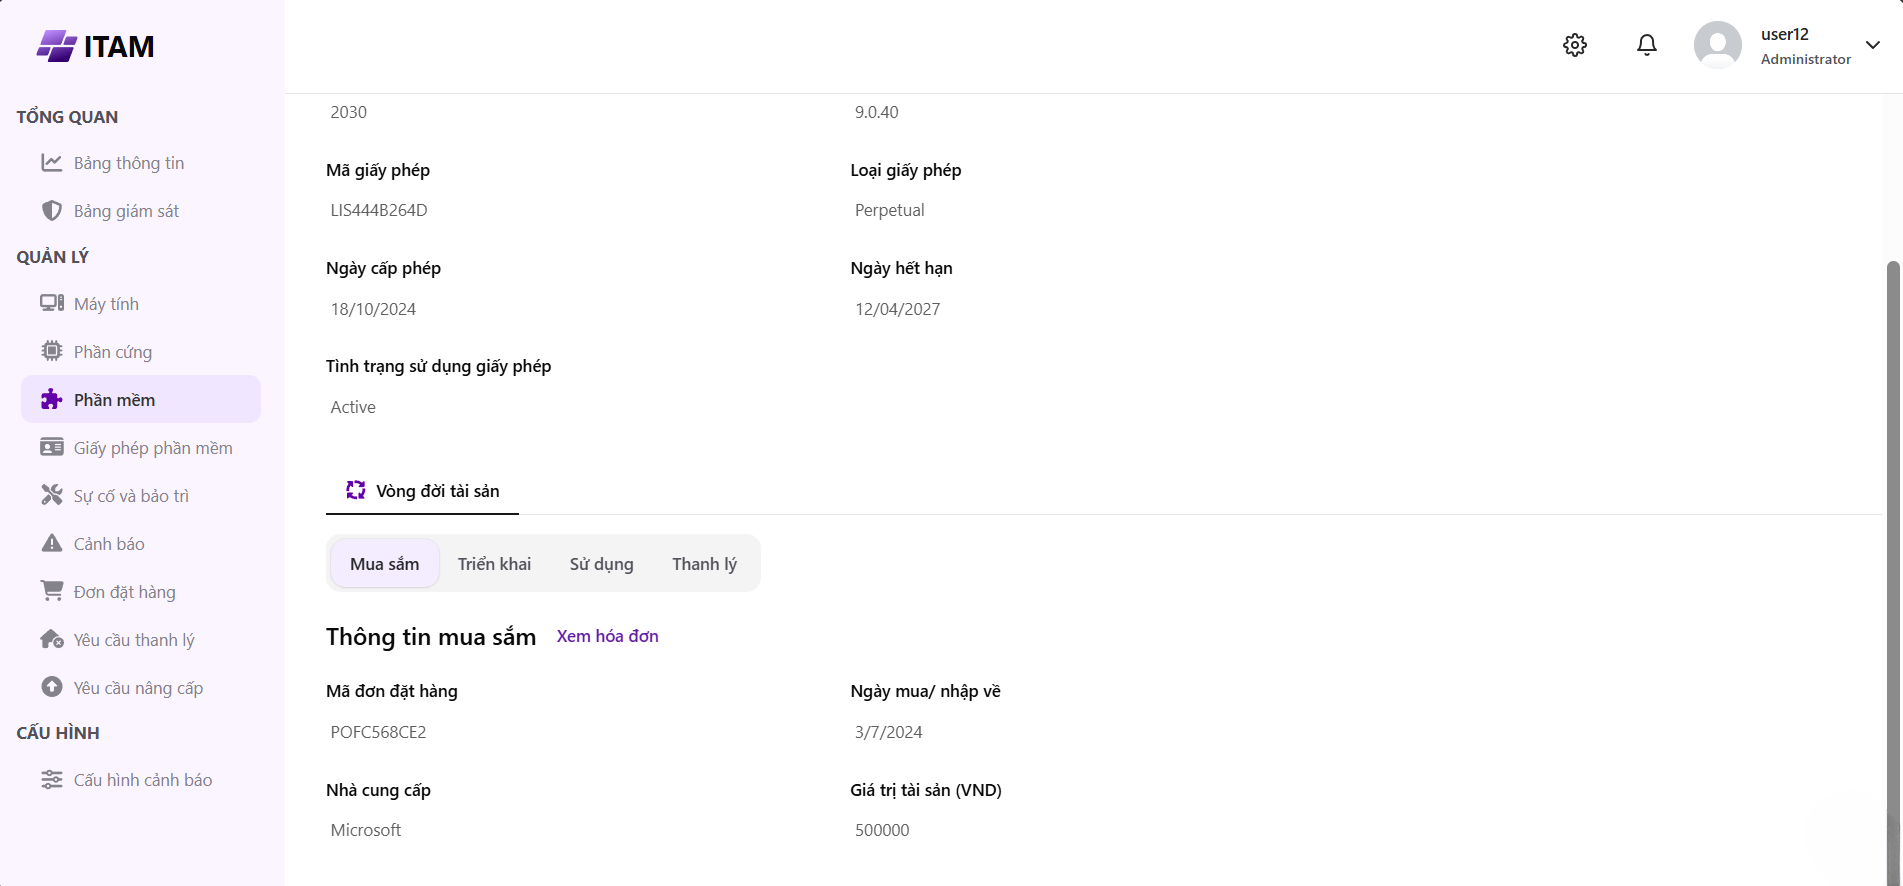
\includegraphics[width=14cm]{Images/C6/UI-Hienthuc/phanmem3.png}
        \vspace{15pt}
        \caption{Giao diện hiện thực tính năng Quản lý phần mềm - vòng đời}
    \end{figure}
    \begin{figure}[H]
        \centering
        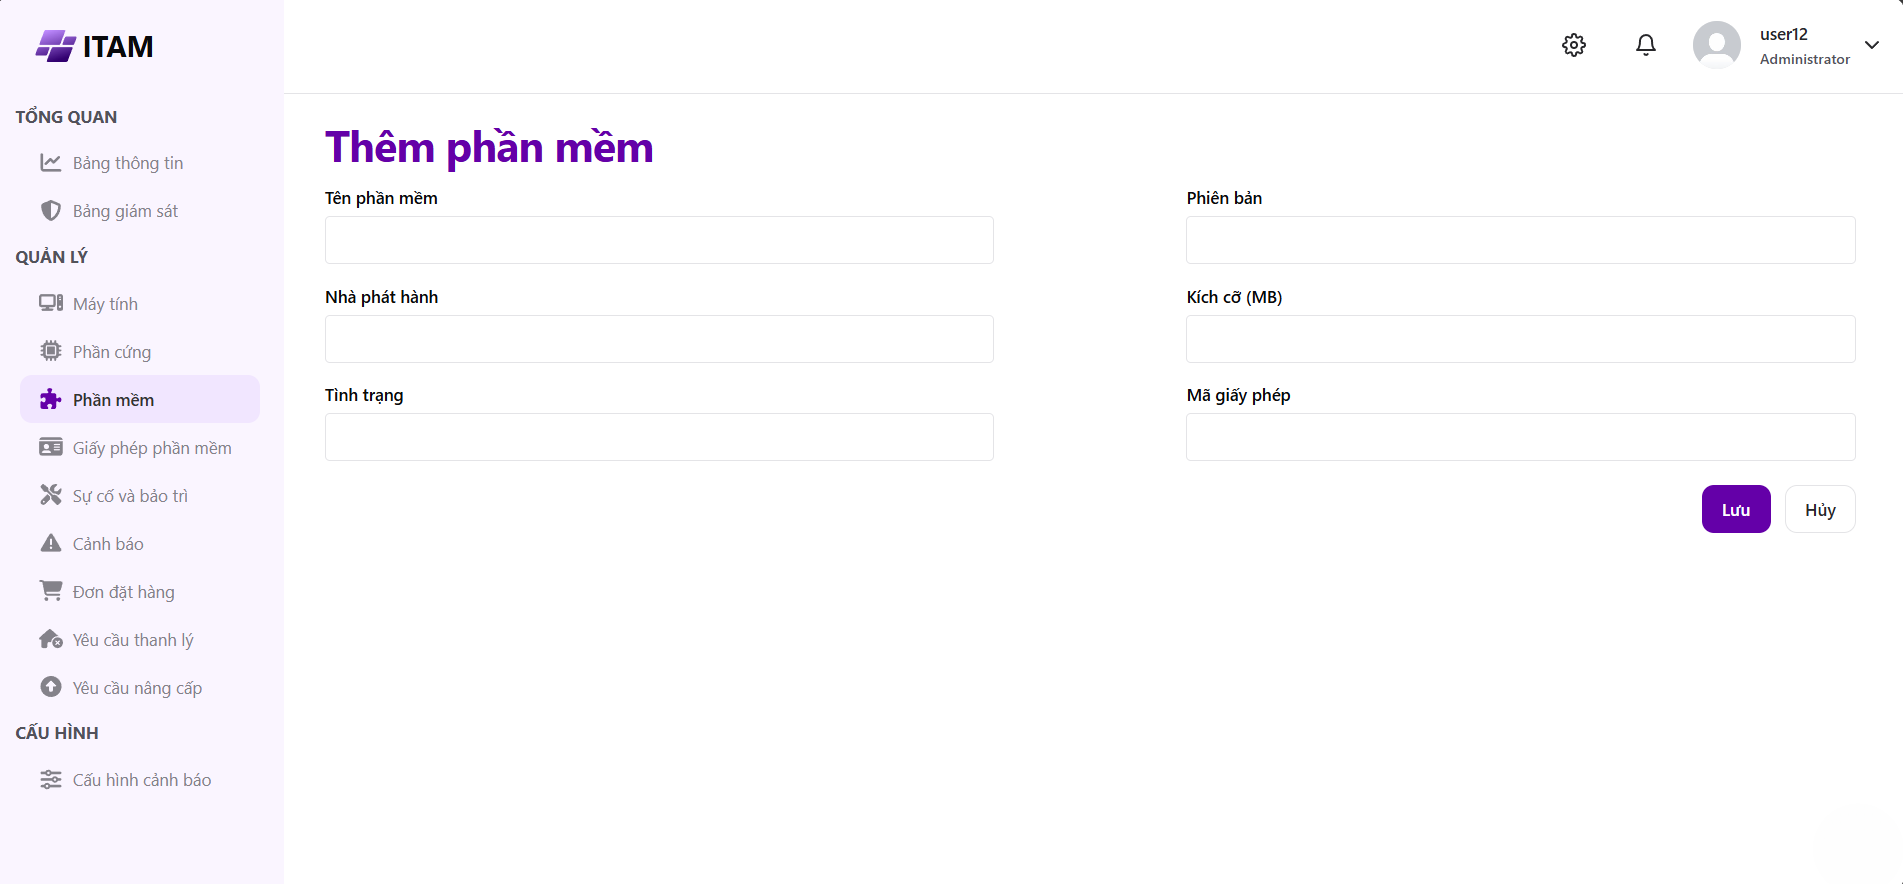
\includegraphics[width=14cm]{Images/C6/UI-Hienthuc/phanmem4.png}
        \vspace{15pt}
        \caption{Giao diện hiện thực tính năng Quản lý phần mềm - thêm phần mềm}
    \end{figure}

    \item Hiện thực tính năng Quản lý Giấy phép phần mềm
    \begin{figure}[H]
        \centering
        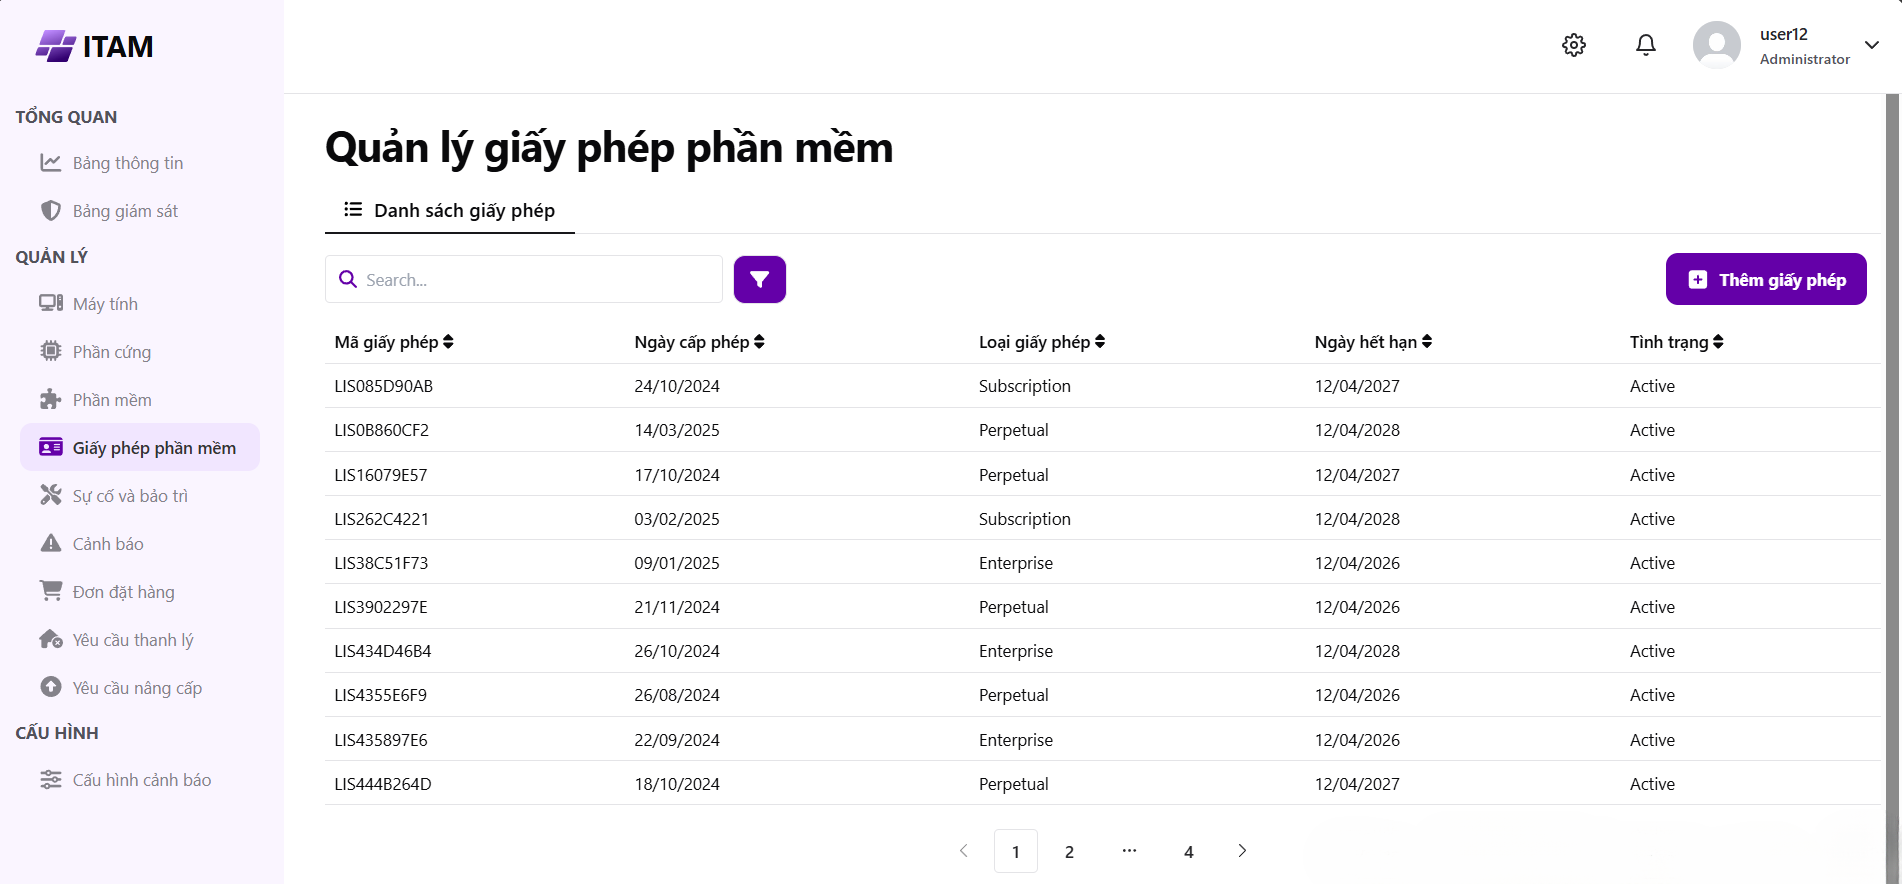
\includegraphics[width=14cm]{Images/C6/UI-Hienthuc/license1.png}
        \vspace{15pt}
        \caption{Giao diện hiện thực tính năng Quản lý Giấy phép phần mềm - danh sách}
    \end{figure}
    \begin{figure}[H]
        \centering
        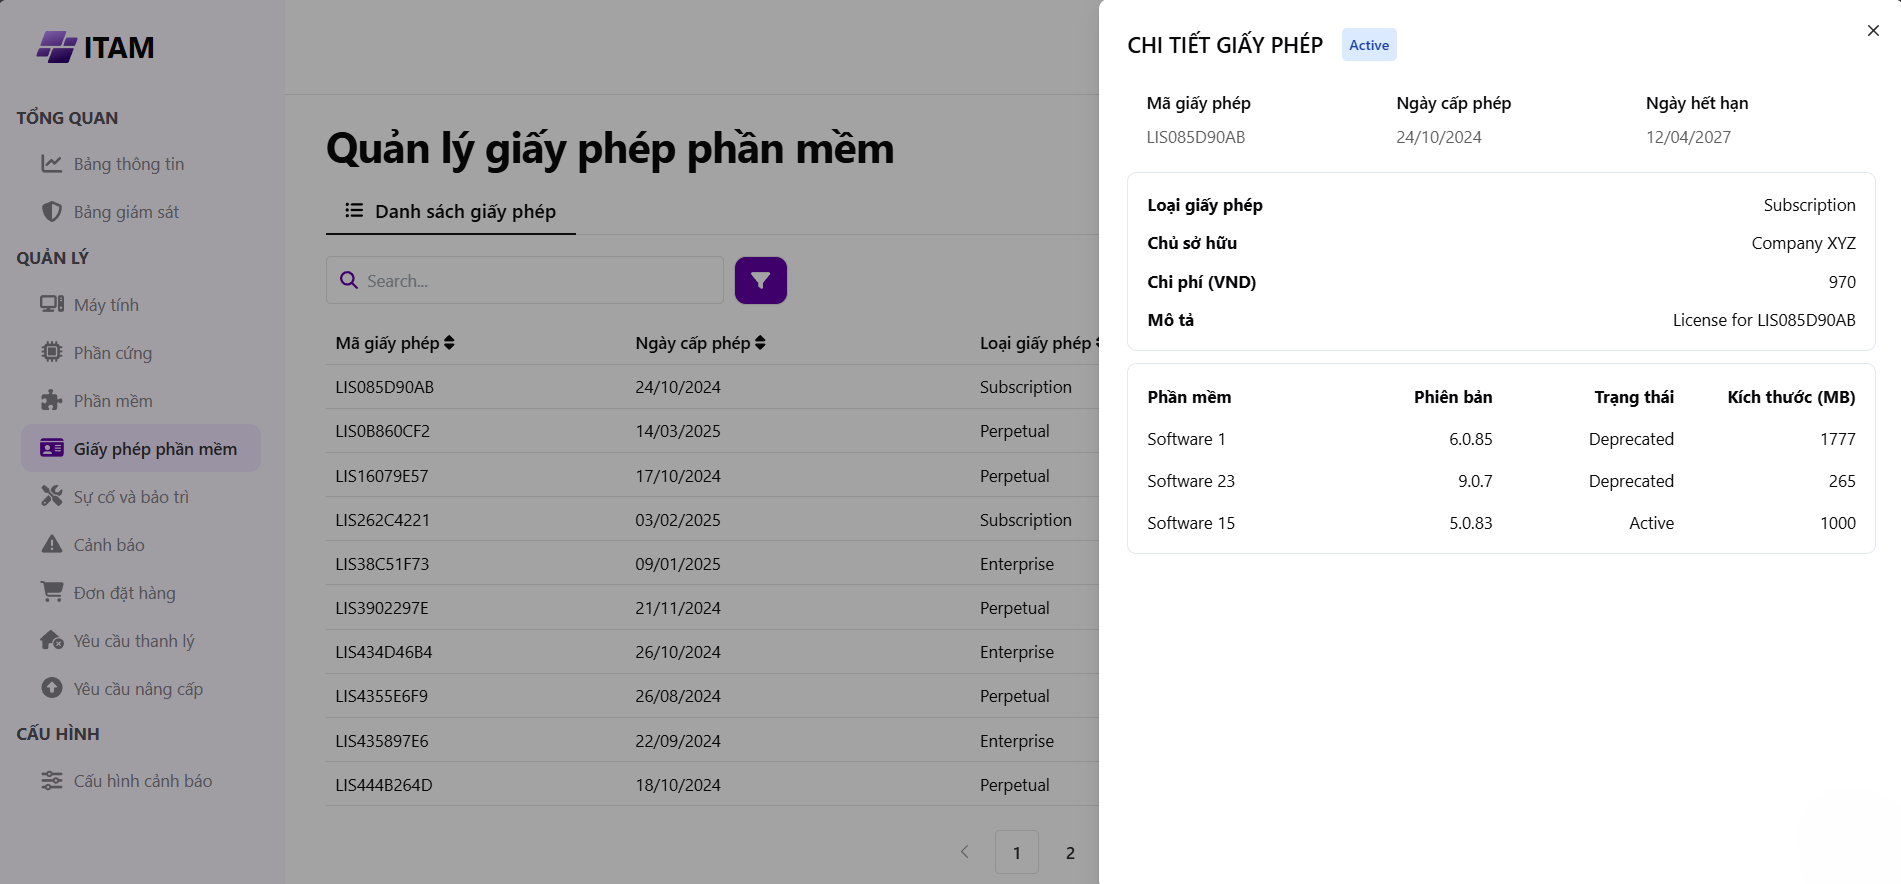
\includegraphics[width=14cm]{Images/C6/UI-Hienthuc/license2.png}
        \vspace{15pt}
        \caption{Giao diện hiện thực tính năng Quản lý Giấy phép phần mềm - chi tiết}
    \end{figure}
    \begin{figure}[H]
        \centering
        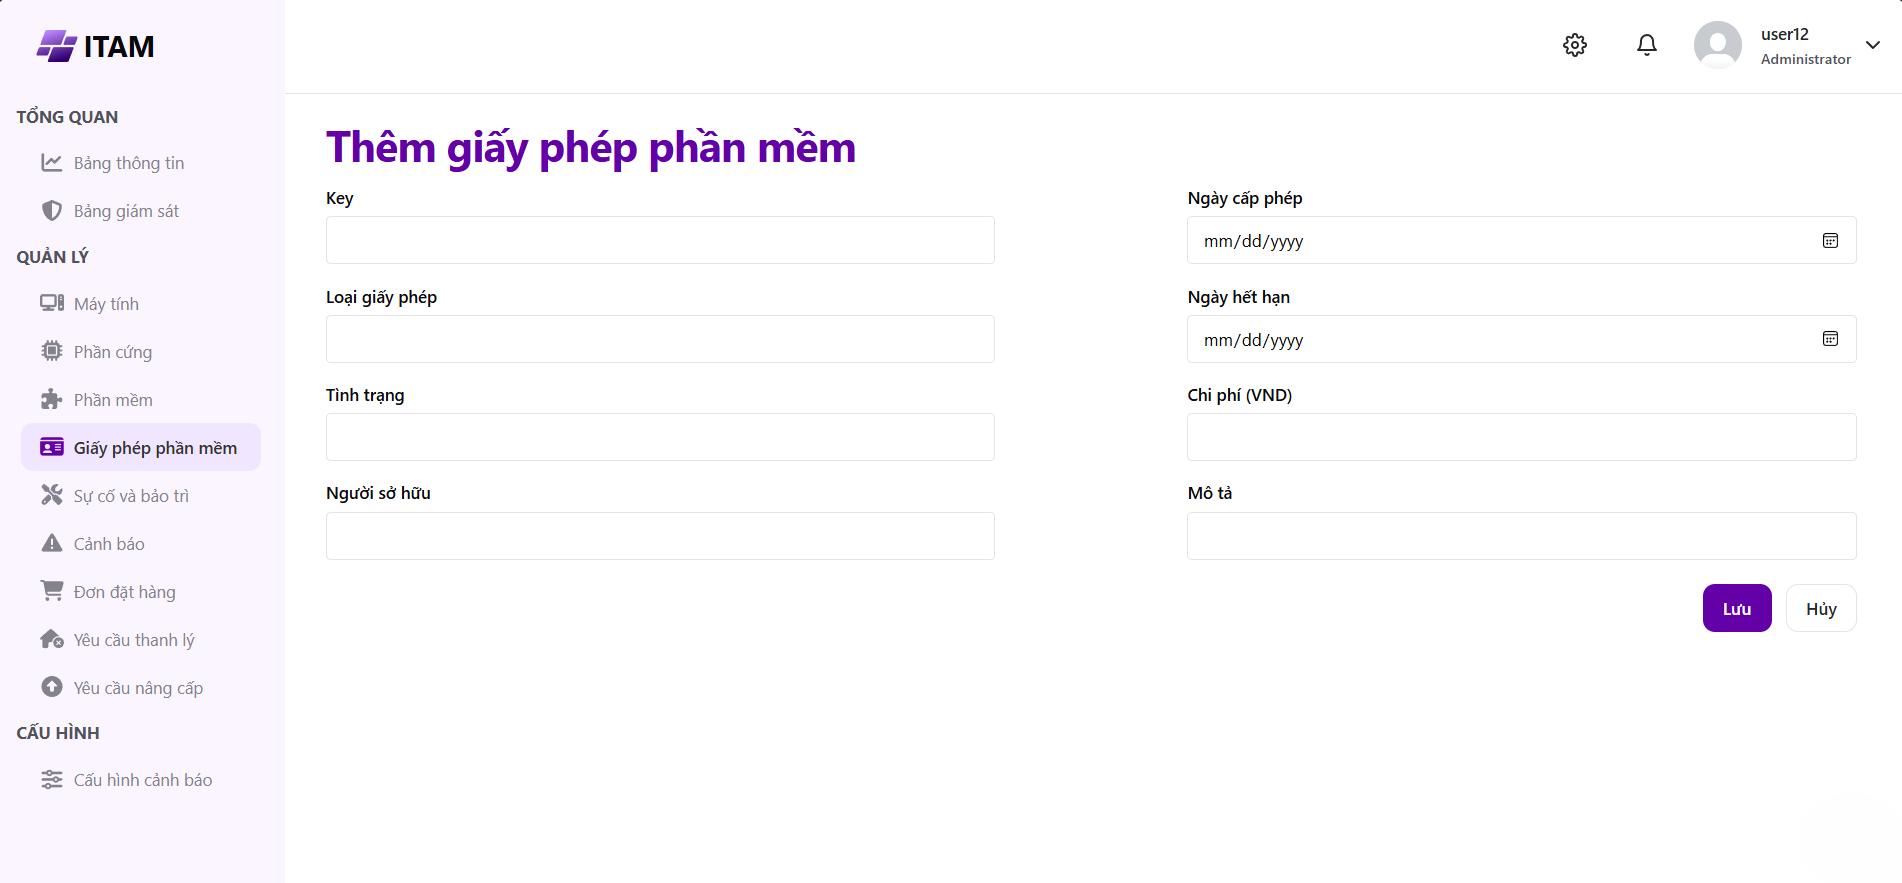
\includegraphics[width=14cm]{Images/C6/UI-Hienthuc/license3.png}
        \vspace{15pt}
        \caption{Giao diện hiện thực tính năng Quản lý Giấy phép phần mềm - thêm giấy phép}
    \end{figure}

    \item Hiện thực tính năng Quản lý Sự cố và bảo trì
    \begin{figure}[H]
        \centering
        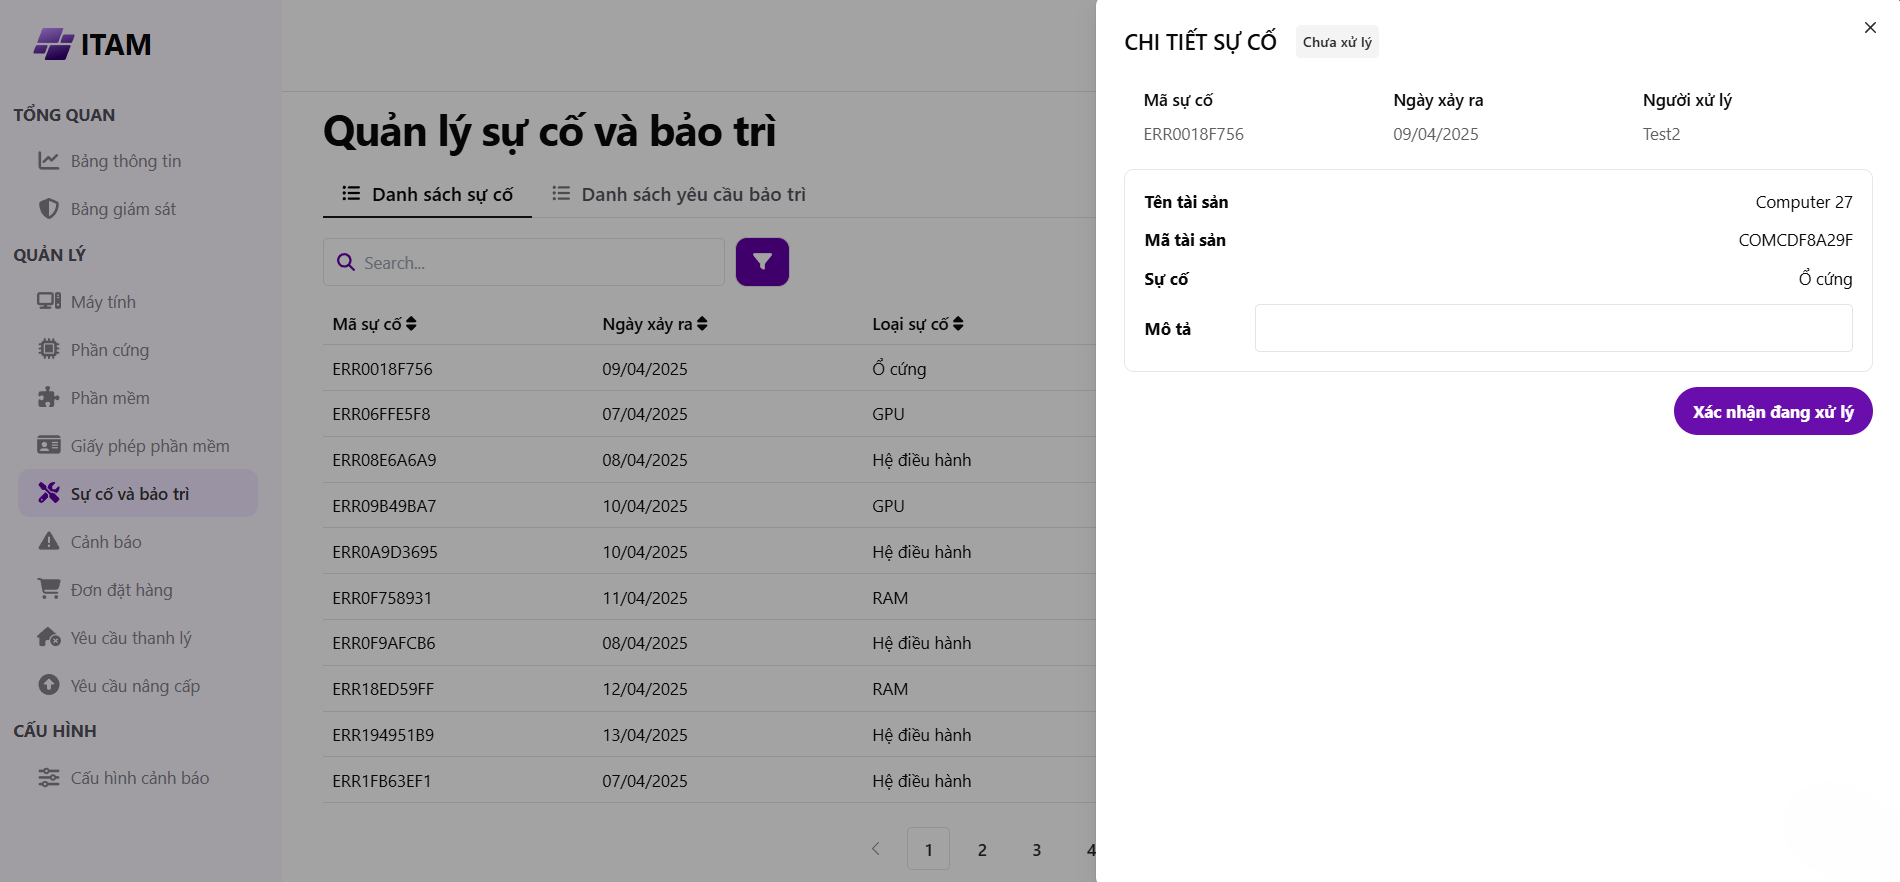
\includegraphics[width=14cm]{Images/C6/UI-Hienthuc/sucobaotri1.png}
        \vspace{15pt}
        \caption{Giao diện hiện thực tính năng Quản lý sự cố}
    \end{figure}
    \begin{figure}[H]
        \centering
        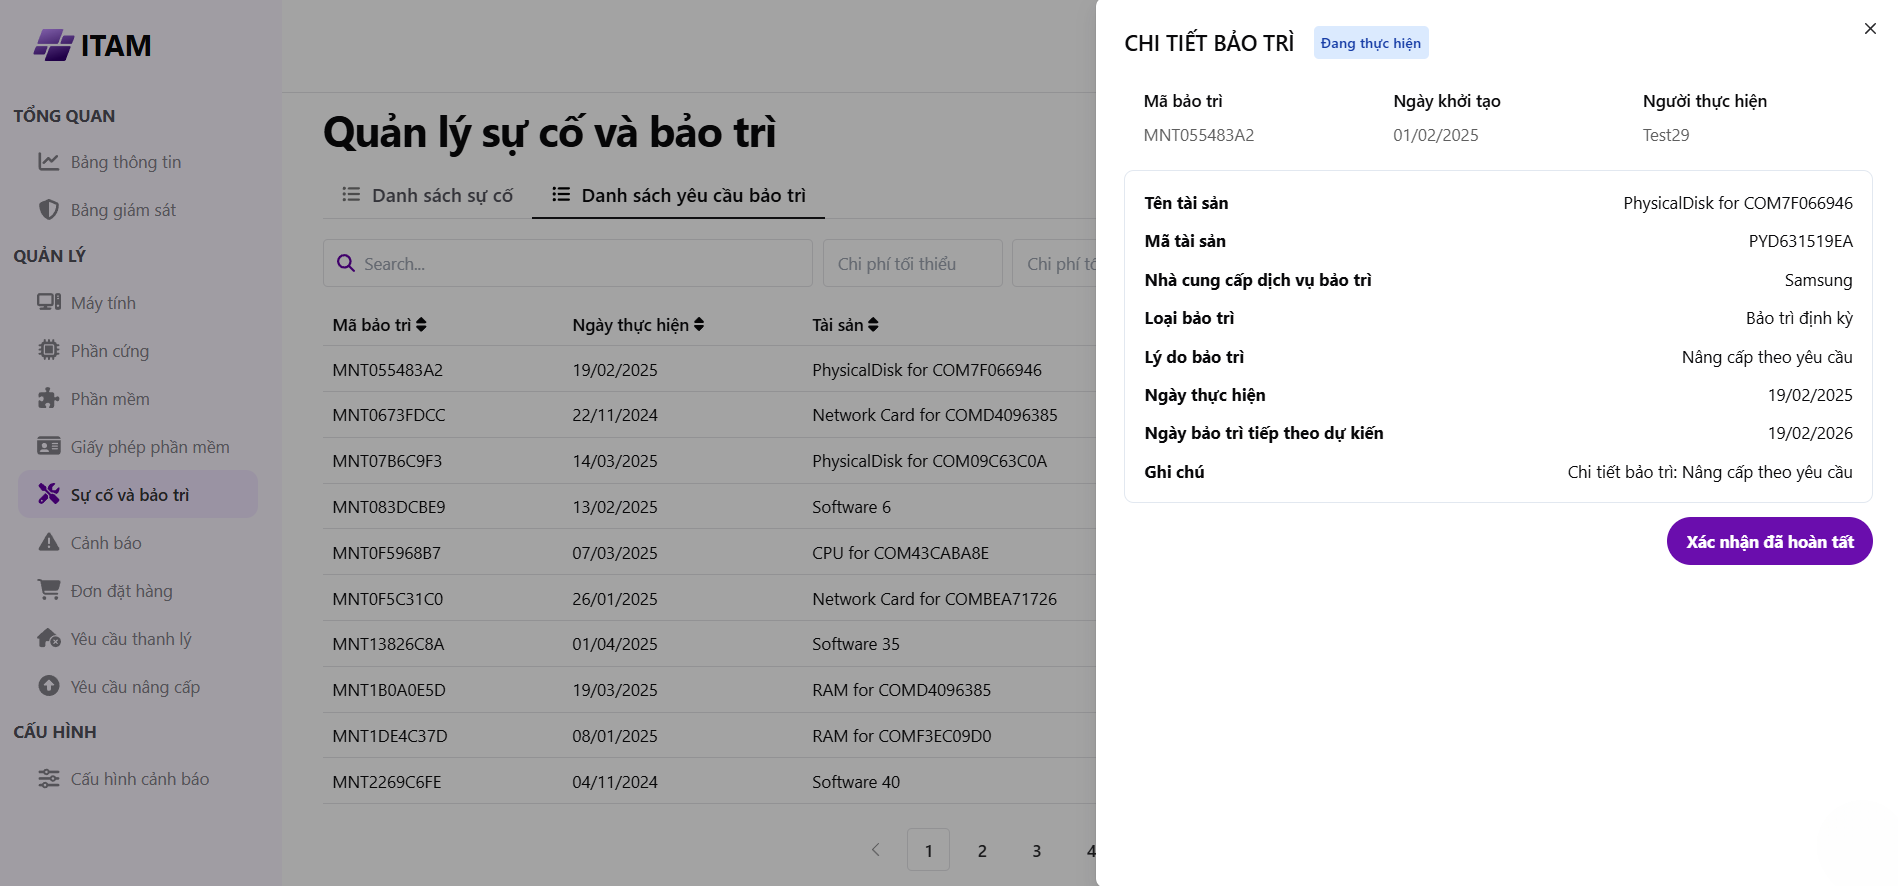
\includegraphics[width=14cm]{Images/C6/UI-Hienthuc/sucobaotri2.png}
        \vspace{15pt}
        \caption{Giao diện hiện thực tính năng Quản lý bảo trì}
    \end{figure}

    \item Hiện thực tính năng Quản lý Cảnh báo
    \begin{figure}[H]
        \centering
        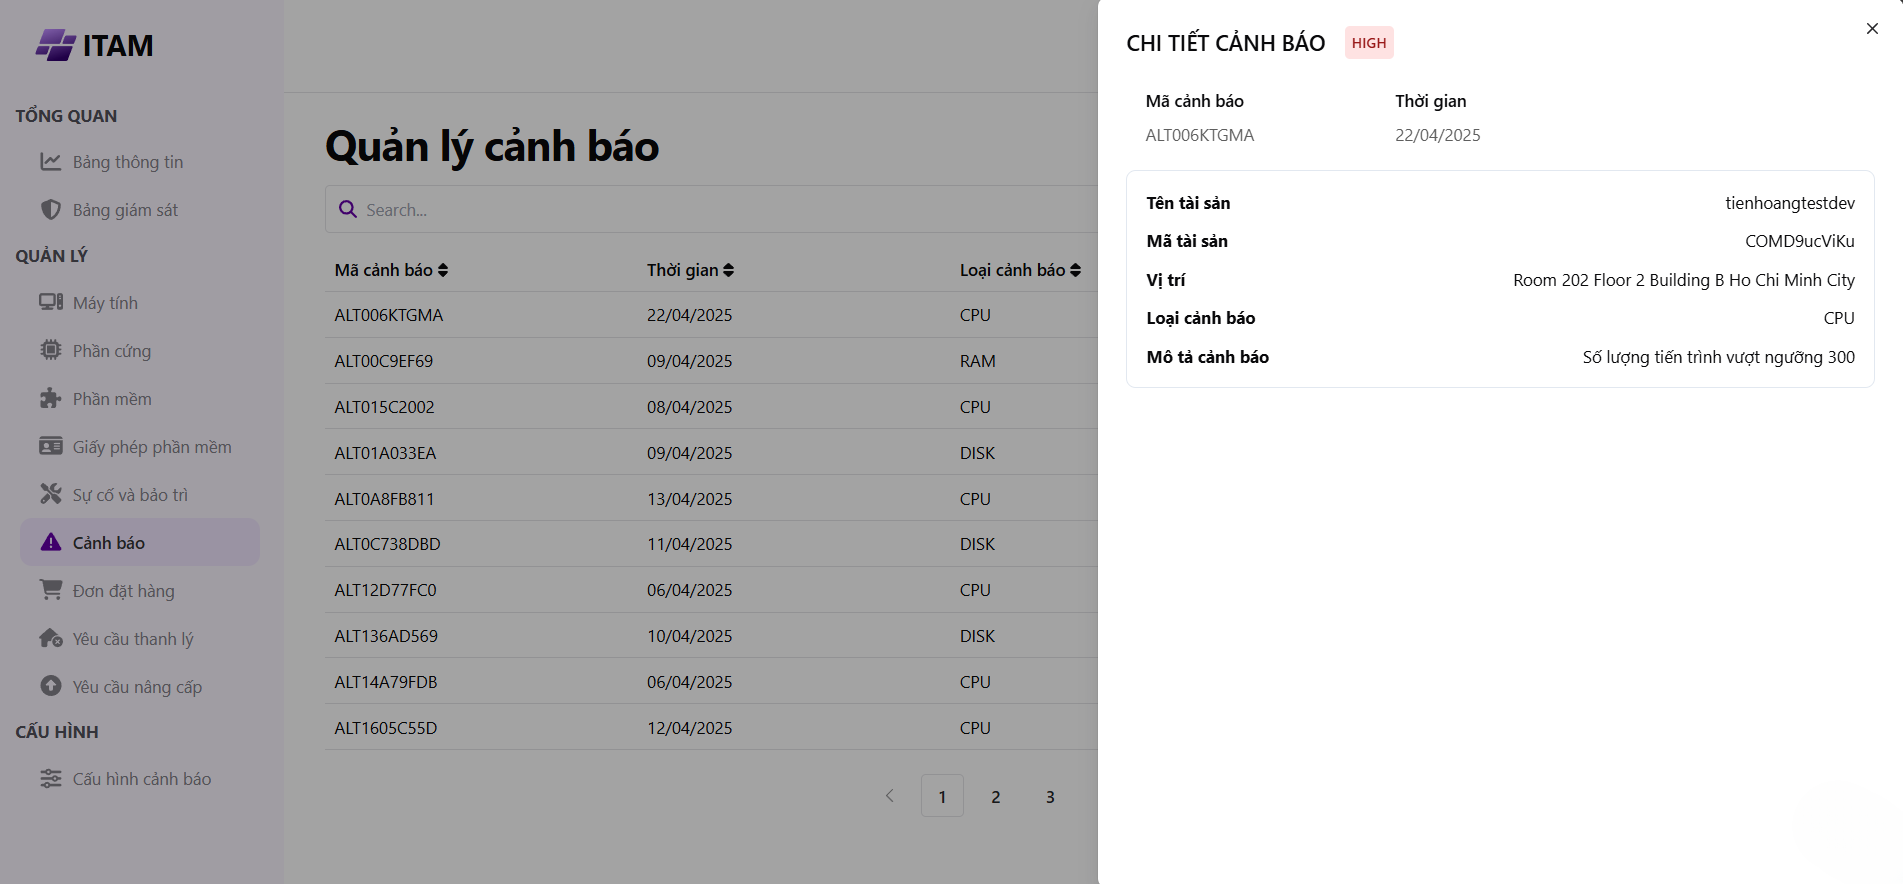
\includegraphics[width=14cm]{Images/C6/UI-Hienthuc/canhbao1.png}
        \vspace{15pt}
        \caption{Giao diện hiện thực tính năng Quản lý Cảnh báo}
    \end{figure}

    \item Hiện thực tính năng Quản lý Đơn đặt hàng
    \begin{figure}[H]
        \centering
        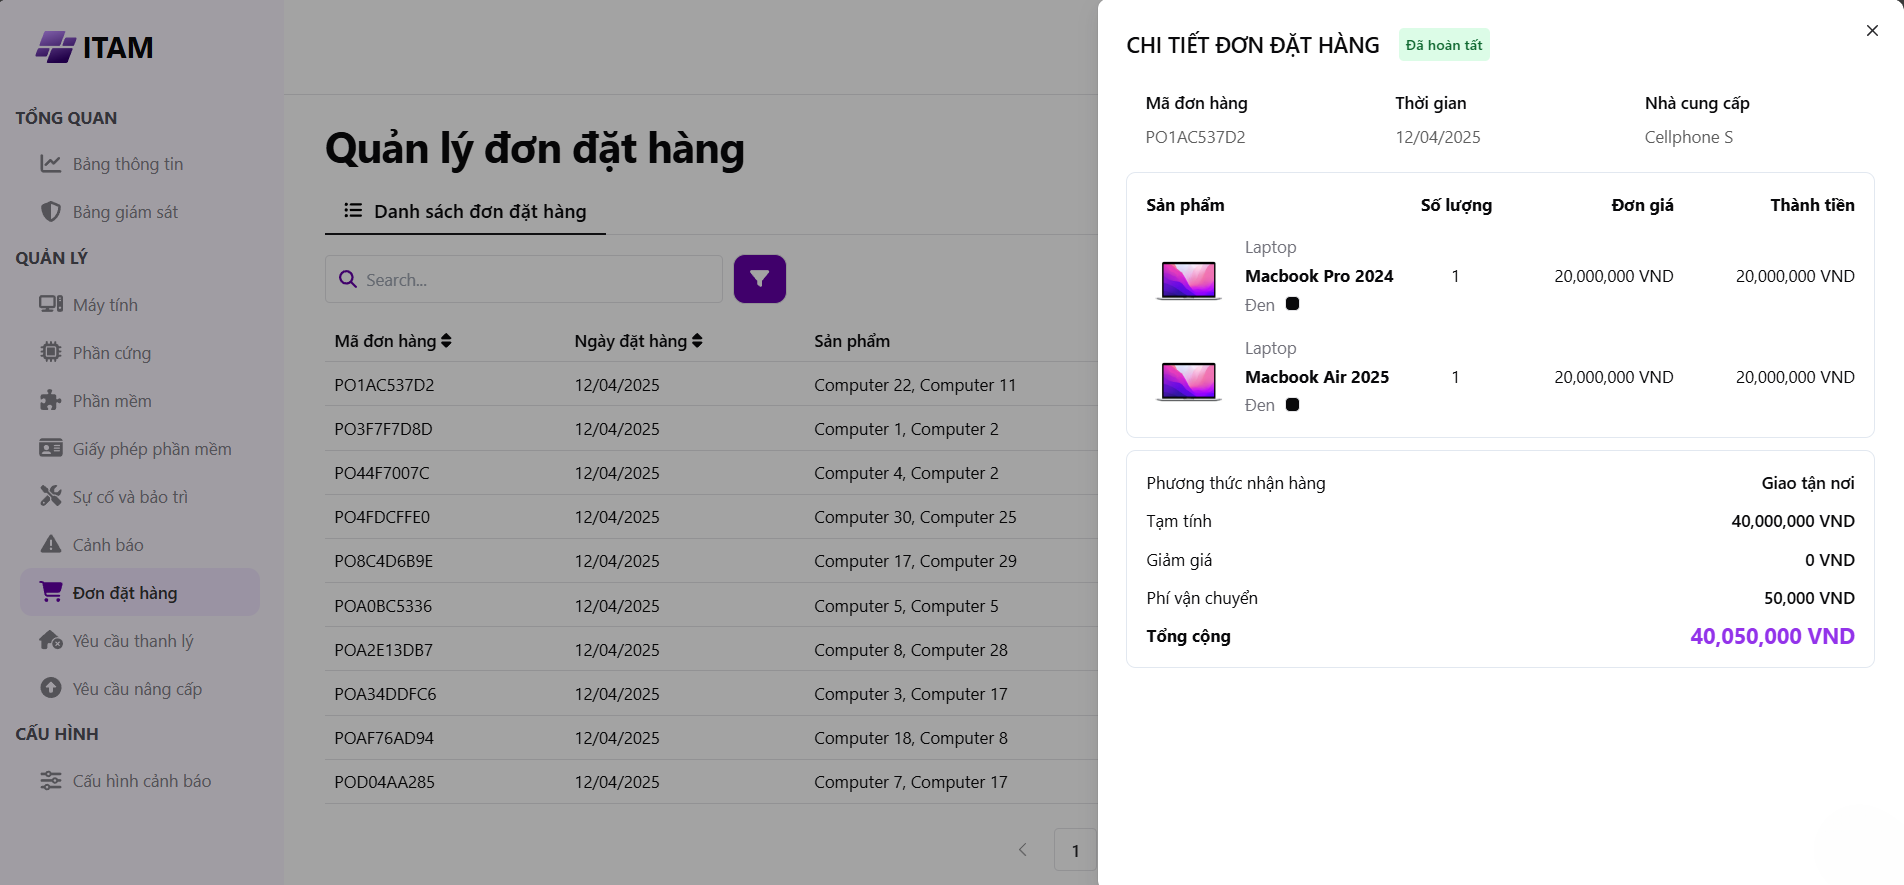
\includegraphics[width=14cm]{Images/C6/UI-Hienthuc/order1.png}
        \vspace{15pt}
        \caption{Giao diện hiện thực tính năng Quản lý Đơn đặt hàng - chi tiết}
    \end{figure}
    \begin{figure}[H]
        \centering
        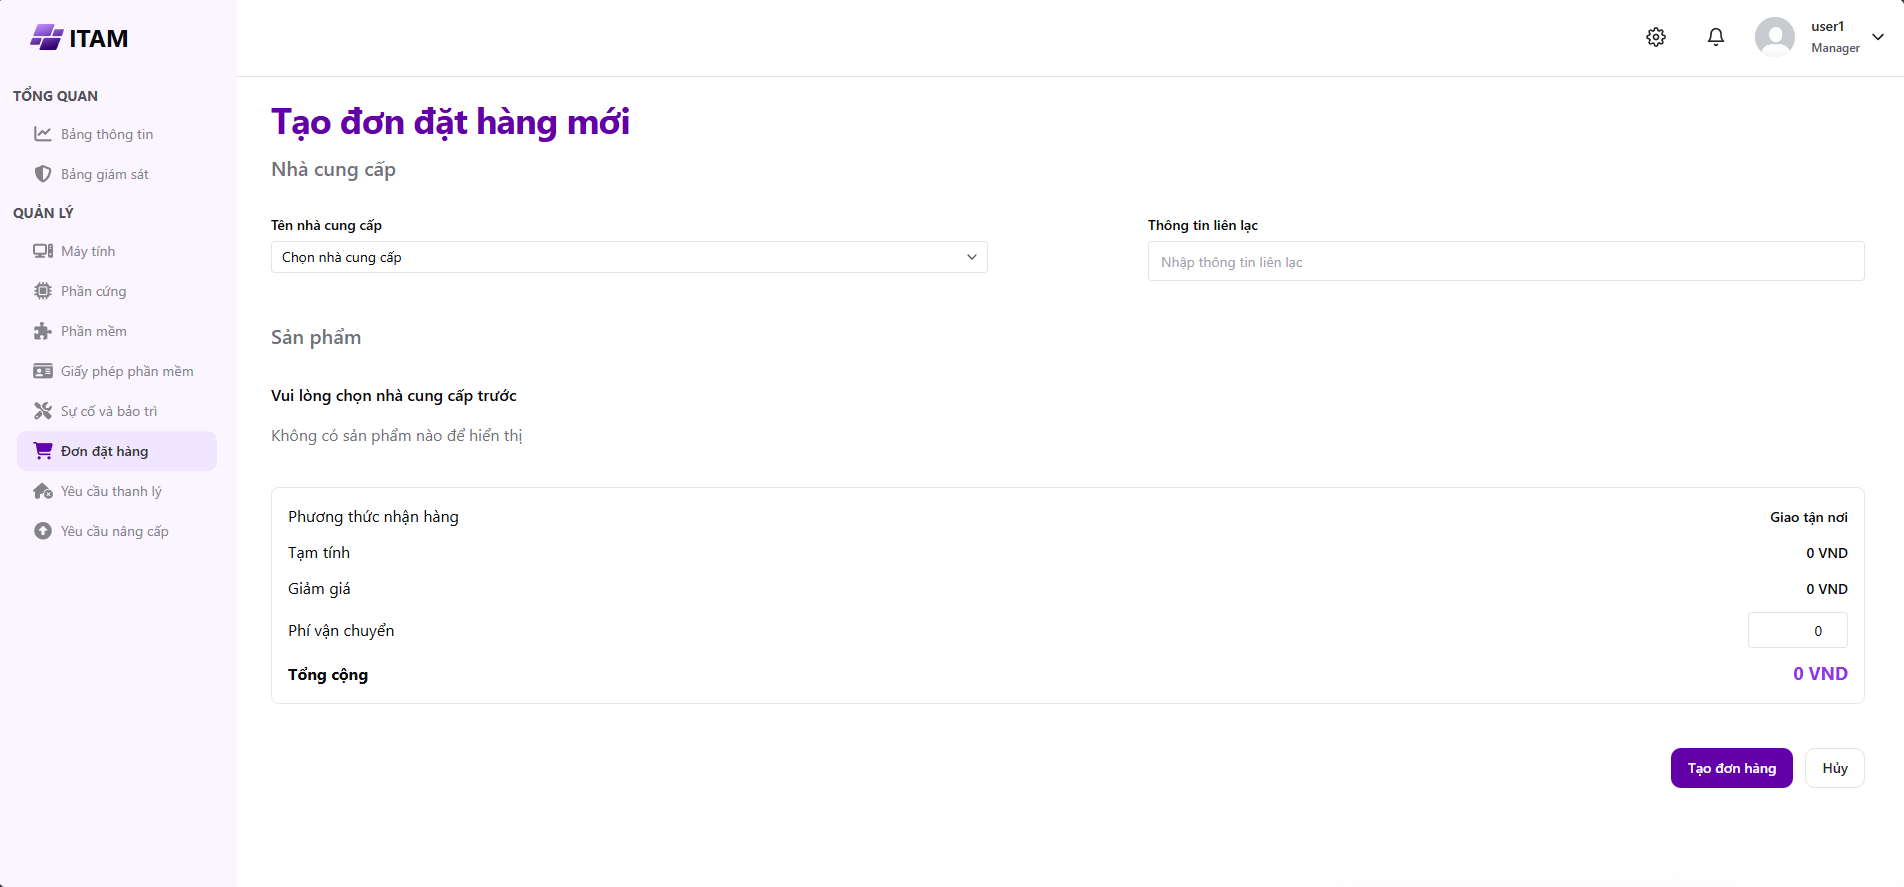
\includegraphics[width=14cm]{Images/C6/UI-Hienthuc/order2.png}
        \vspace{15pt}
        \caption{Giao diện hiện thực tính năng Quản lý Đơn đặt hàng - tạo đơn mới}
    \end{figure}
    \begin{figure}[H]
        \centering
        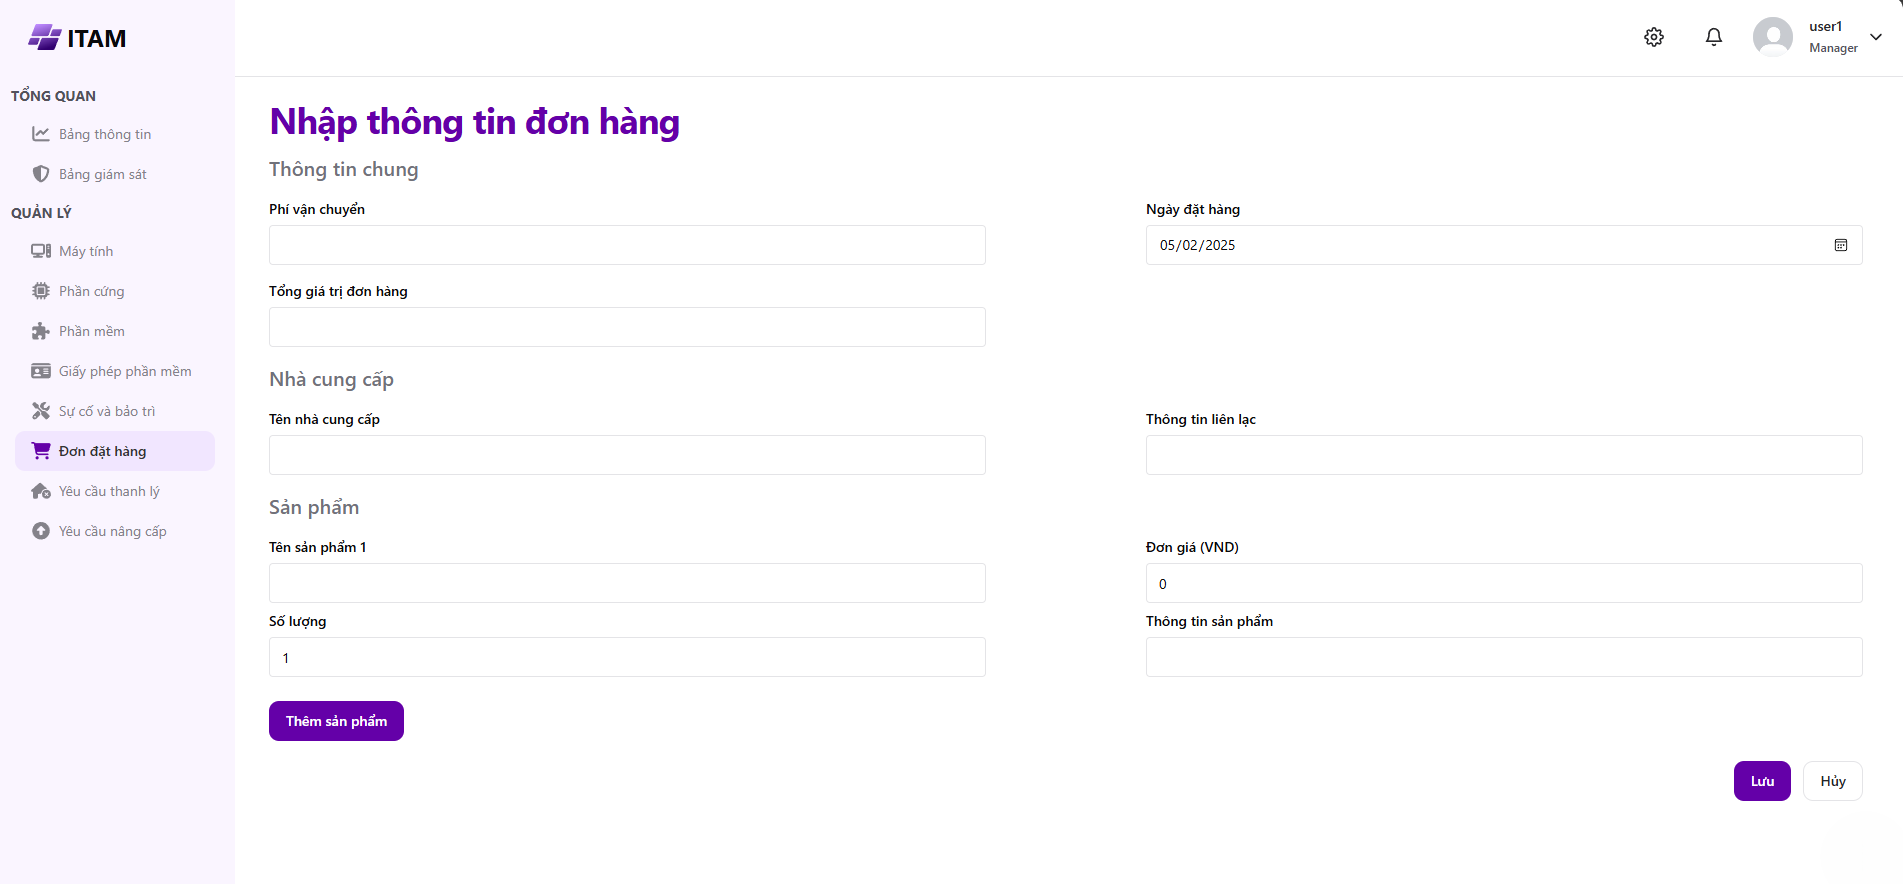
\includegraphics[width=14cm]{Images/C6/UI-Hienthuc/order3.png}
        \vspace{15pt}
        \caption{Giao diện hiện thực tính năng Quản lý Đơn đặt hàng - nhập đơn mới}
    \end{figure}

    \item Hiện thực tính năng Quản lý Yêu cầu nâng cấp, Yêu cầu thanh lý
    \begin{figure}[H]
        \centering
        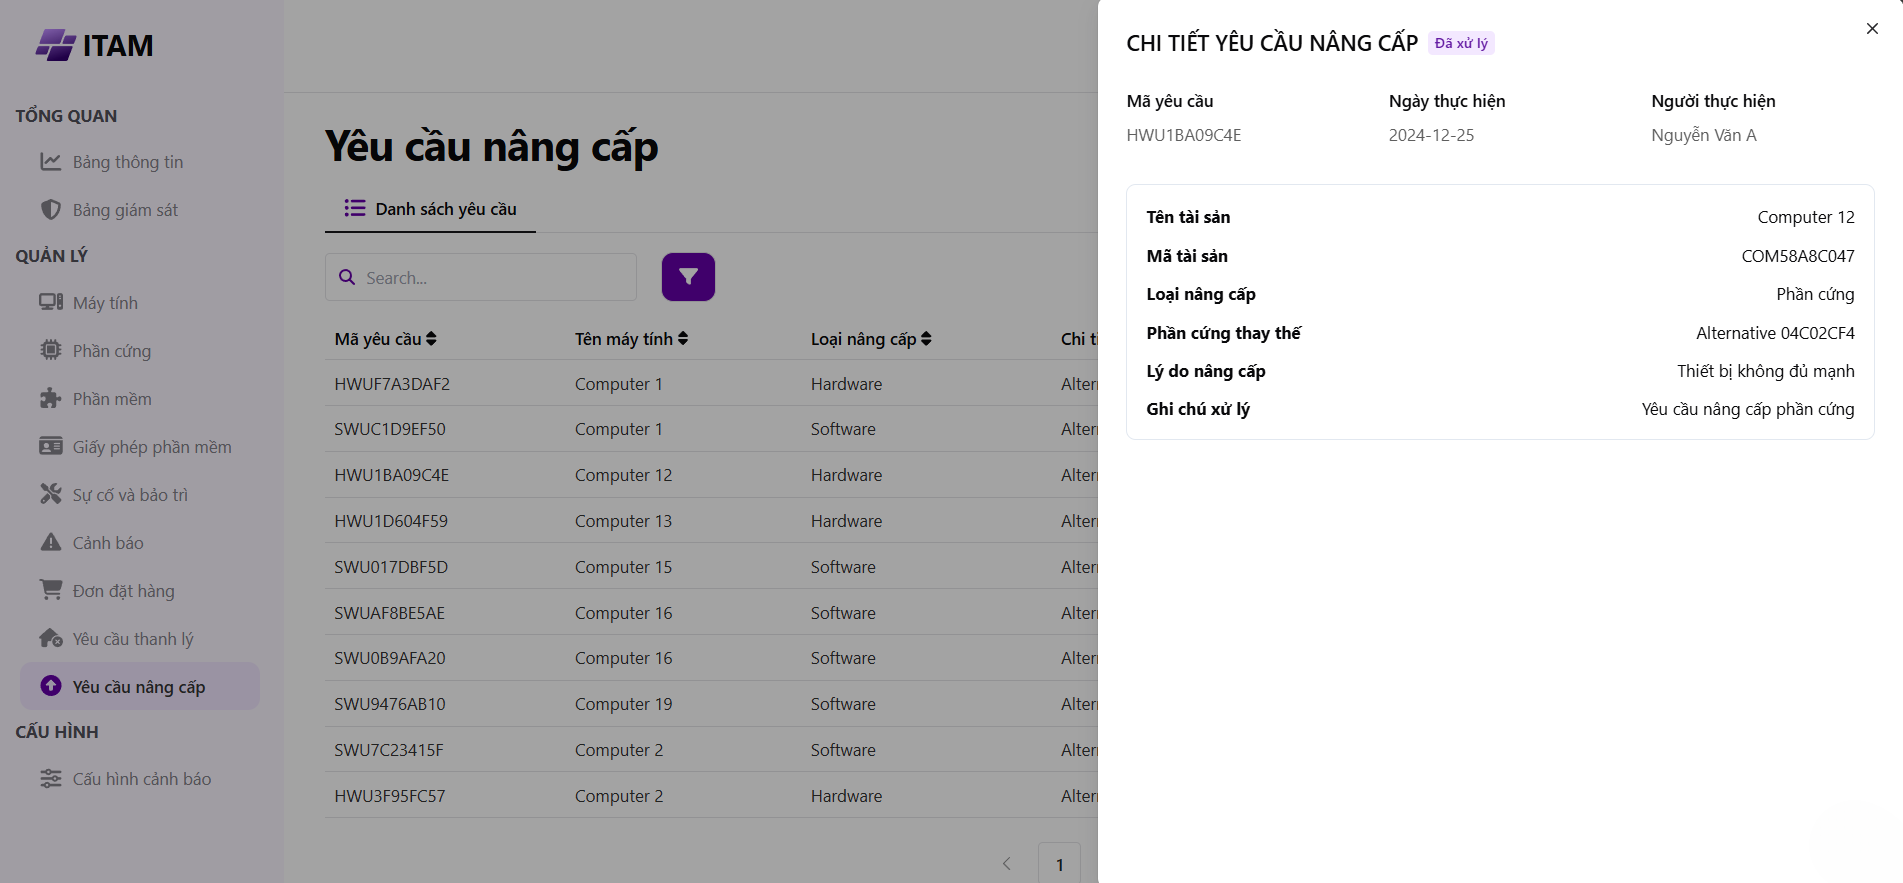
\includegraphics[width=14cm]{Images/C6/UI-Hienthuc/upgrade1.png}
        \vspace{15pt}
        \caption{Giao diện hiện thực tính năng Quản lý Yêu cầu nâng cấp}
    \end{figure}
    \begin{figure}[H]
        \centering
        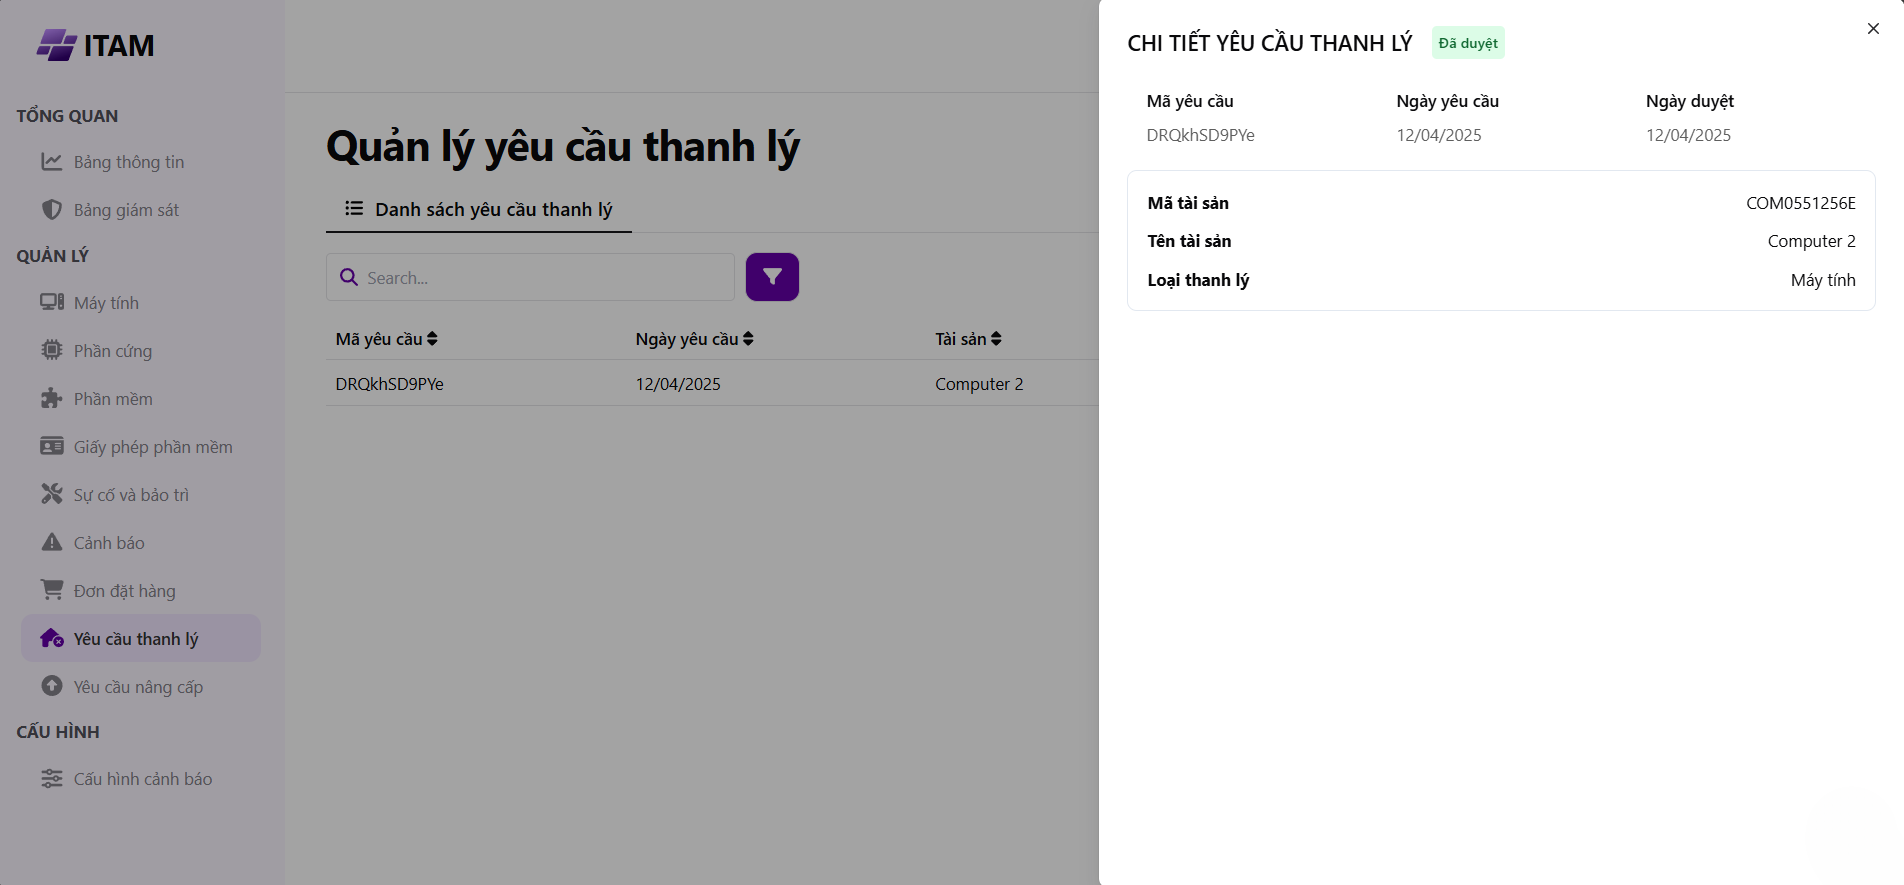
\includegraphics[width=14cm]{Images/C6/UI-Hienthuc/disposal1.png}
        \vspace{15pt}
        \caption{Giao diện hiện thực tính năng Quản lý Yêu cầu thanh lý}
    \end{figure}

    \item Hiện thực tính năng Cấu hình cảnh báo
    \begin{figure}[H]
        \centering
        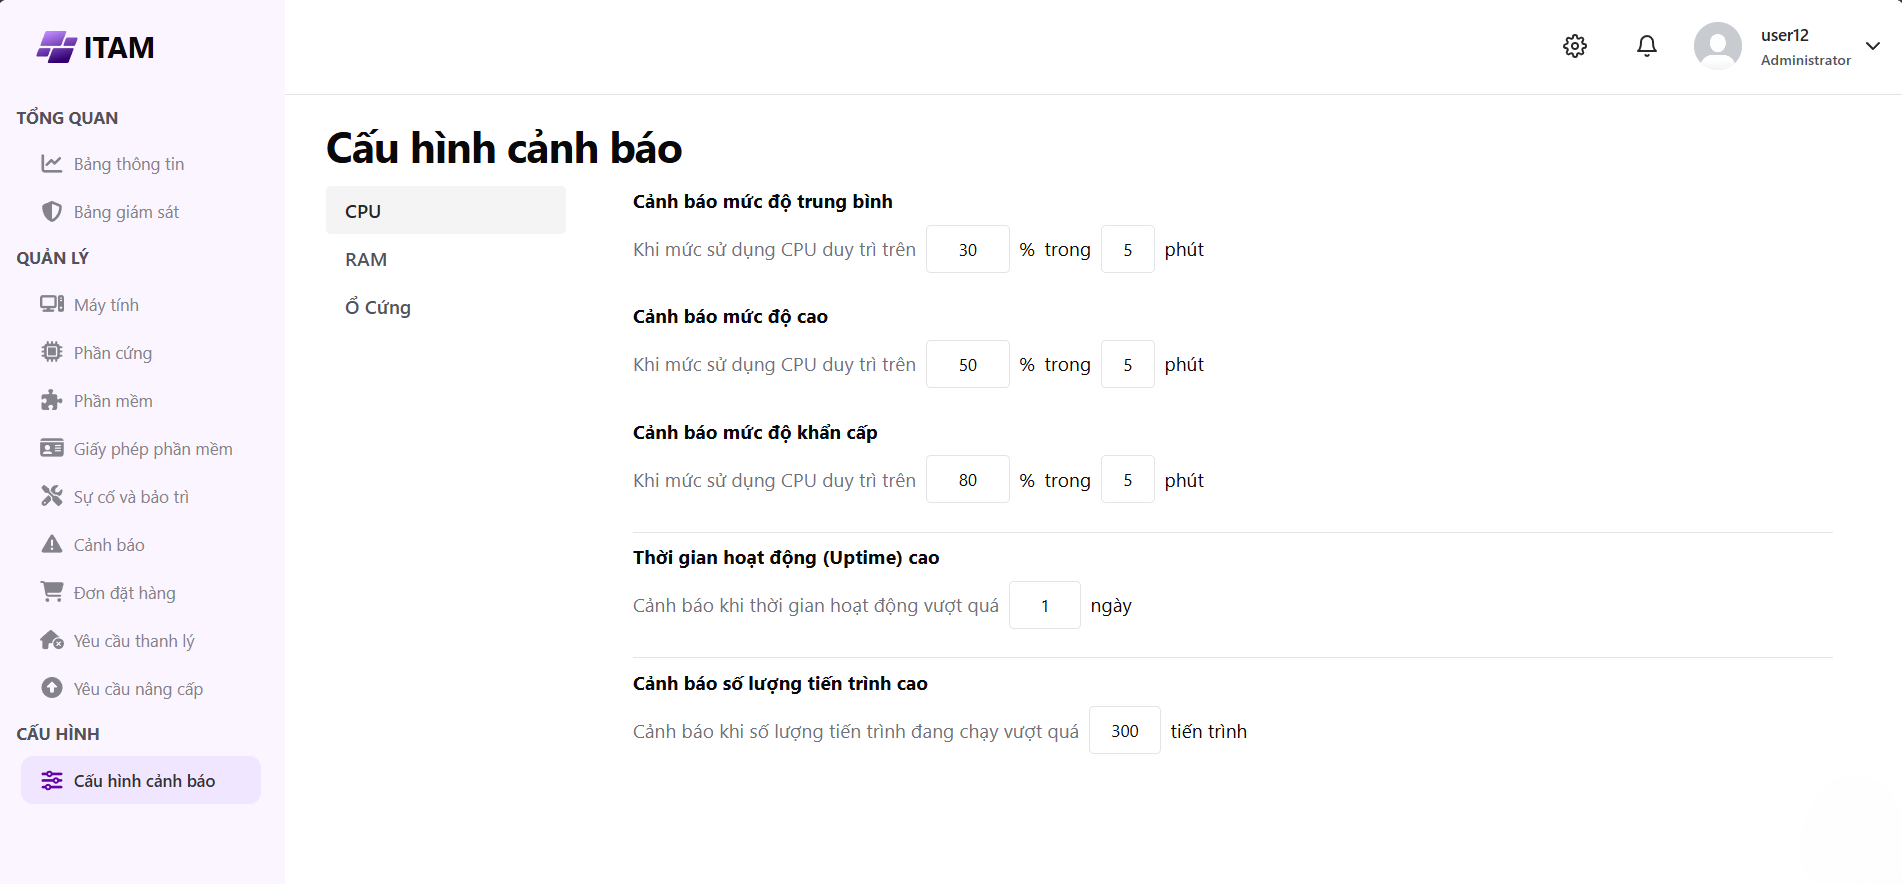
\includegraphics[width=14cm]{Images/C6/UI-Hienthuc/settings1.png}
        \vspace{15pt}
        \caption{Giao diện hiện thực tính năng Cấu hình cảnh báo}
    \end{figure}

    \item Hiện thực tính năng Báo cáo tổng quan
    \begin{figure}[H]
        \centering
        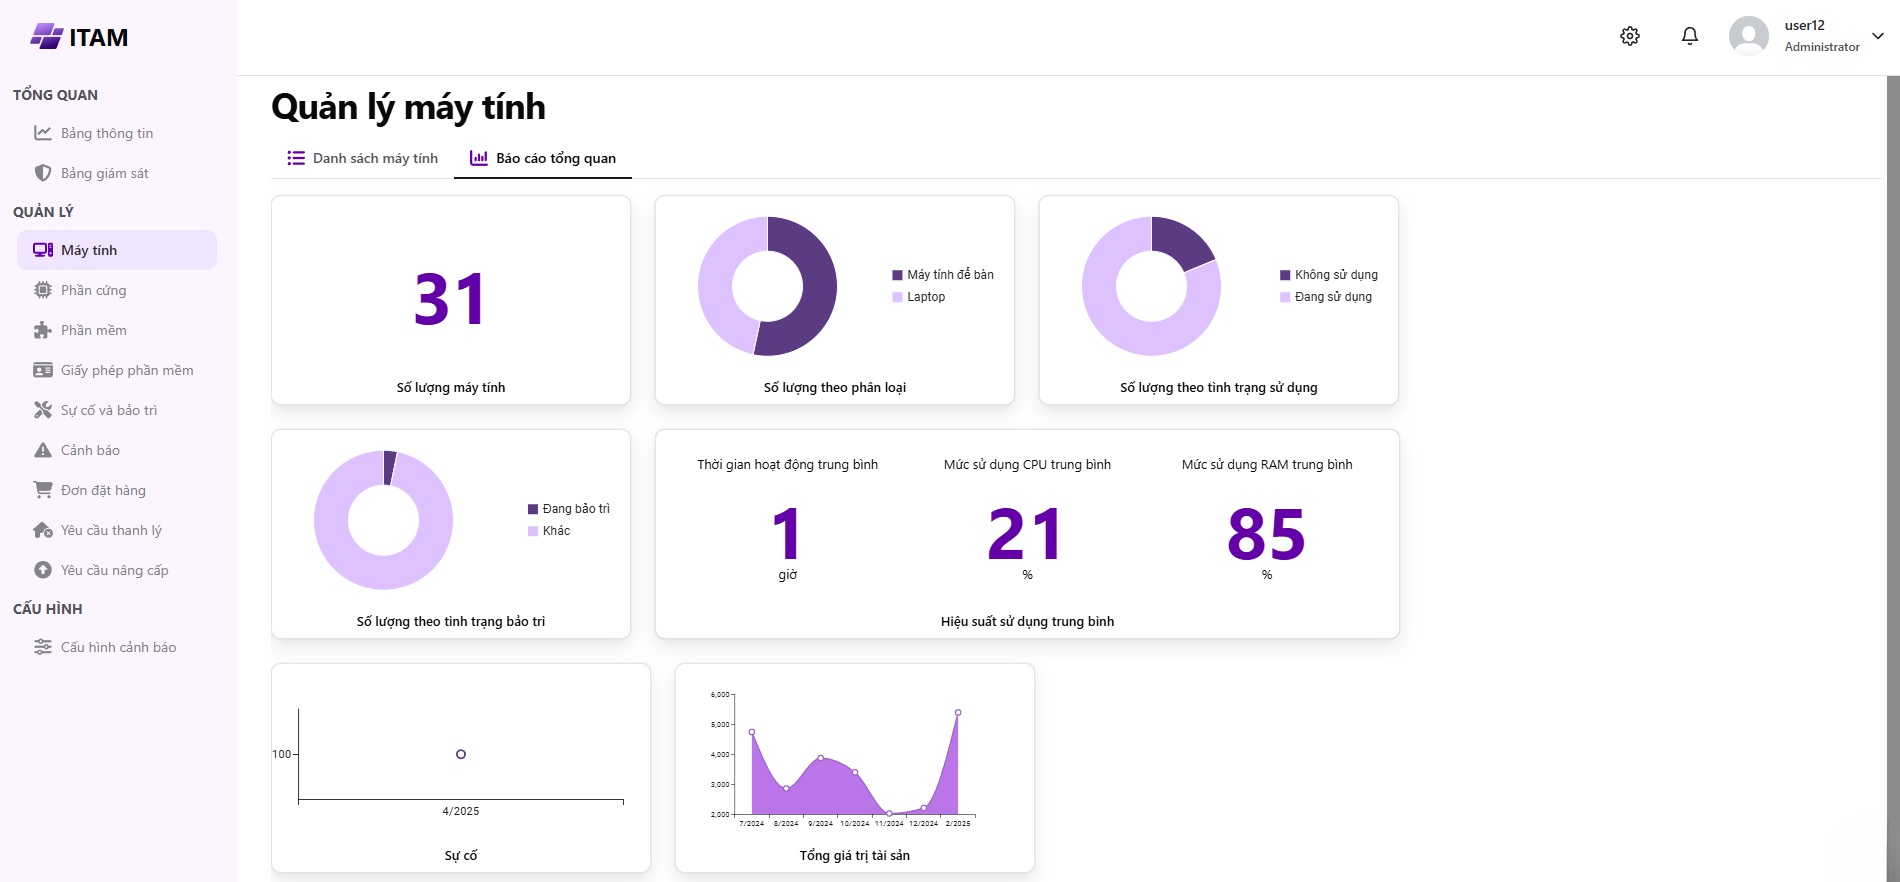
\includegraphics[width=14cm]{Images/C6/UI-Hienthuc/overview1.png}
        \vspace{15pt}
        \caption{Giao diện hiện thực tính năng Báo cáo tổng quan - máy tính}
    \end{figure}
    \begin{figure}[H]
        \centering
        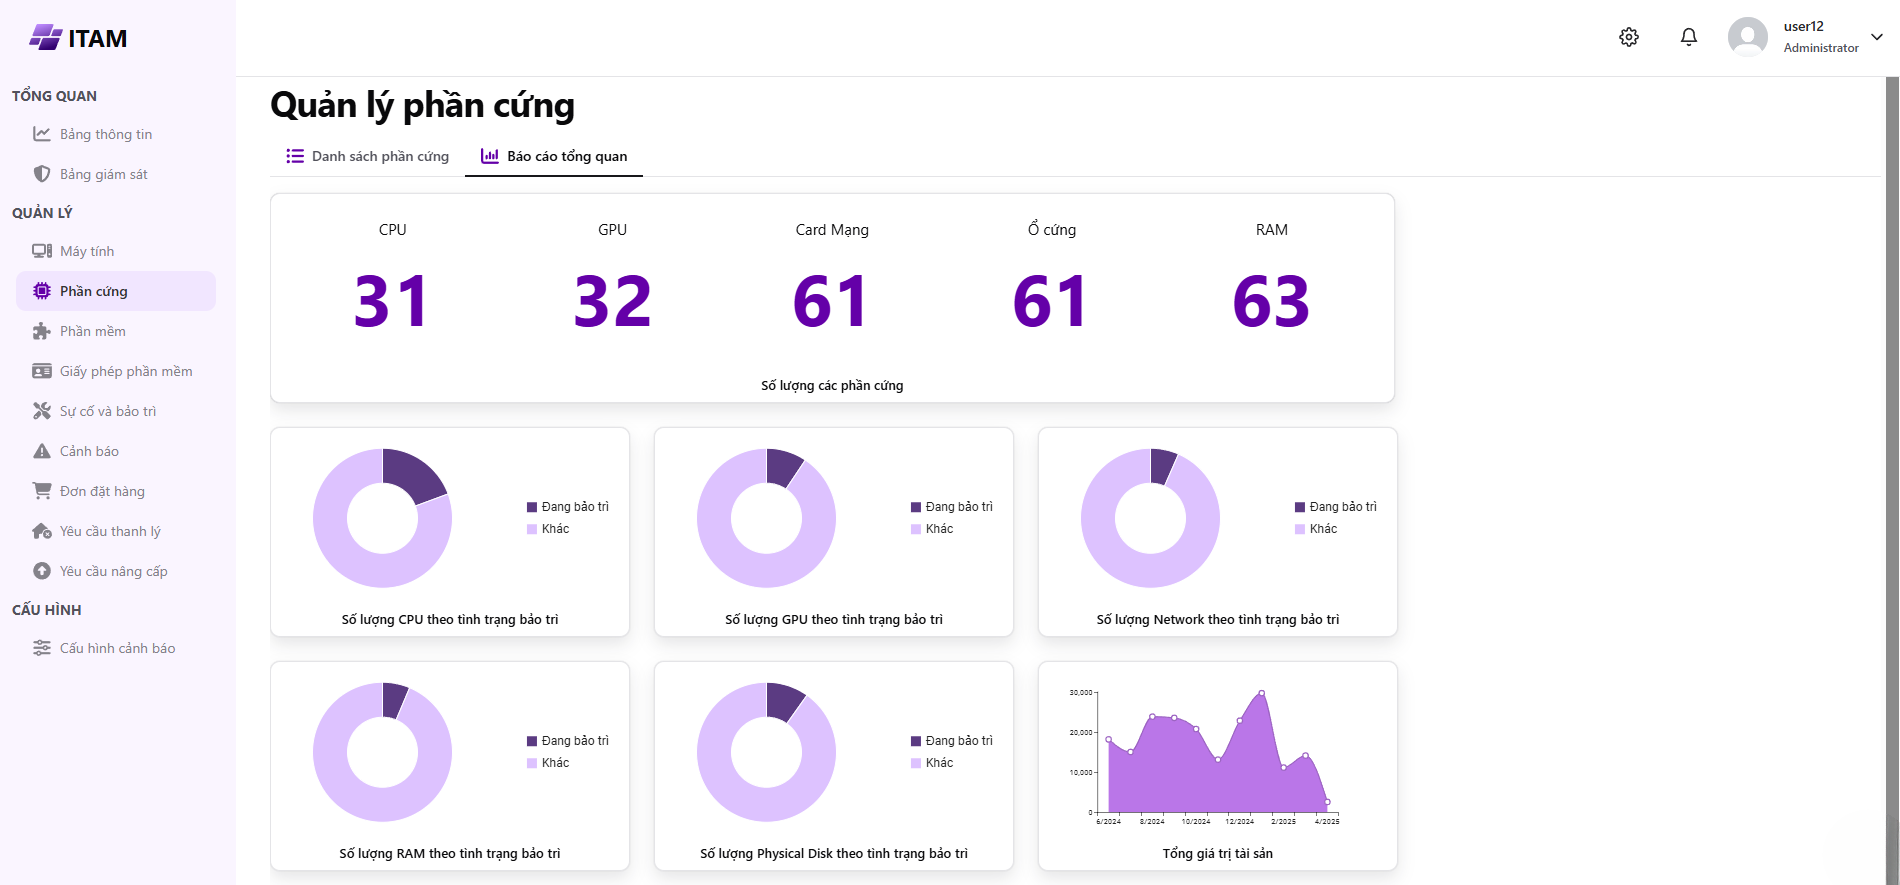
\includegraphics[width=14cm]{Images/C6/UI-Hienthuc/overview2.png}
        \vspace{15pt}
        \caption{Giao diện hiện thực tính năng Báo cáo tổng quan - phần cứng}
    \end{figure}
    \begin{figure}[H]
        \centering
        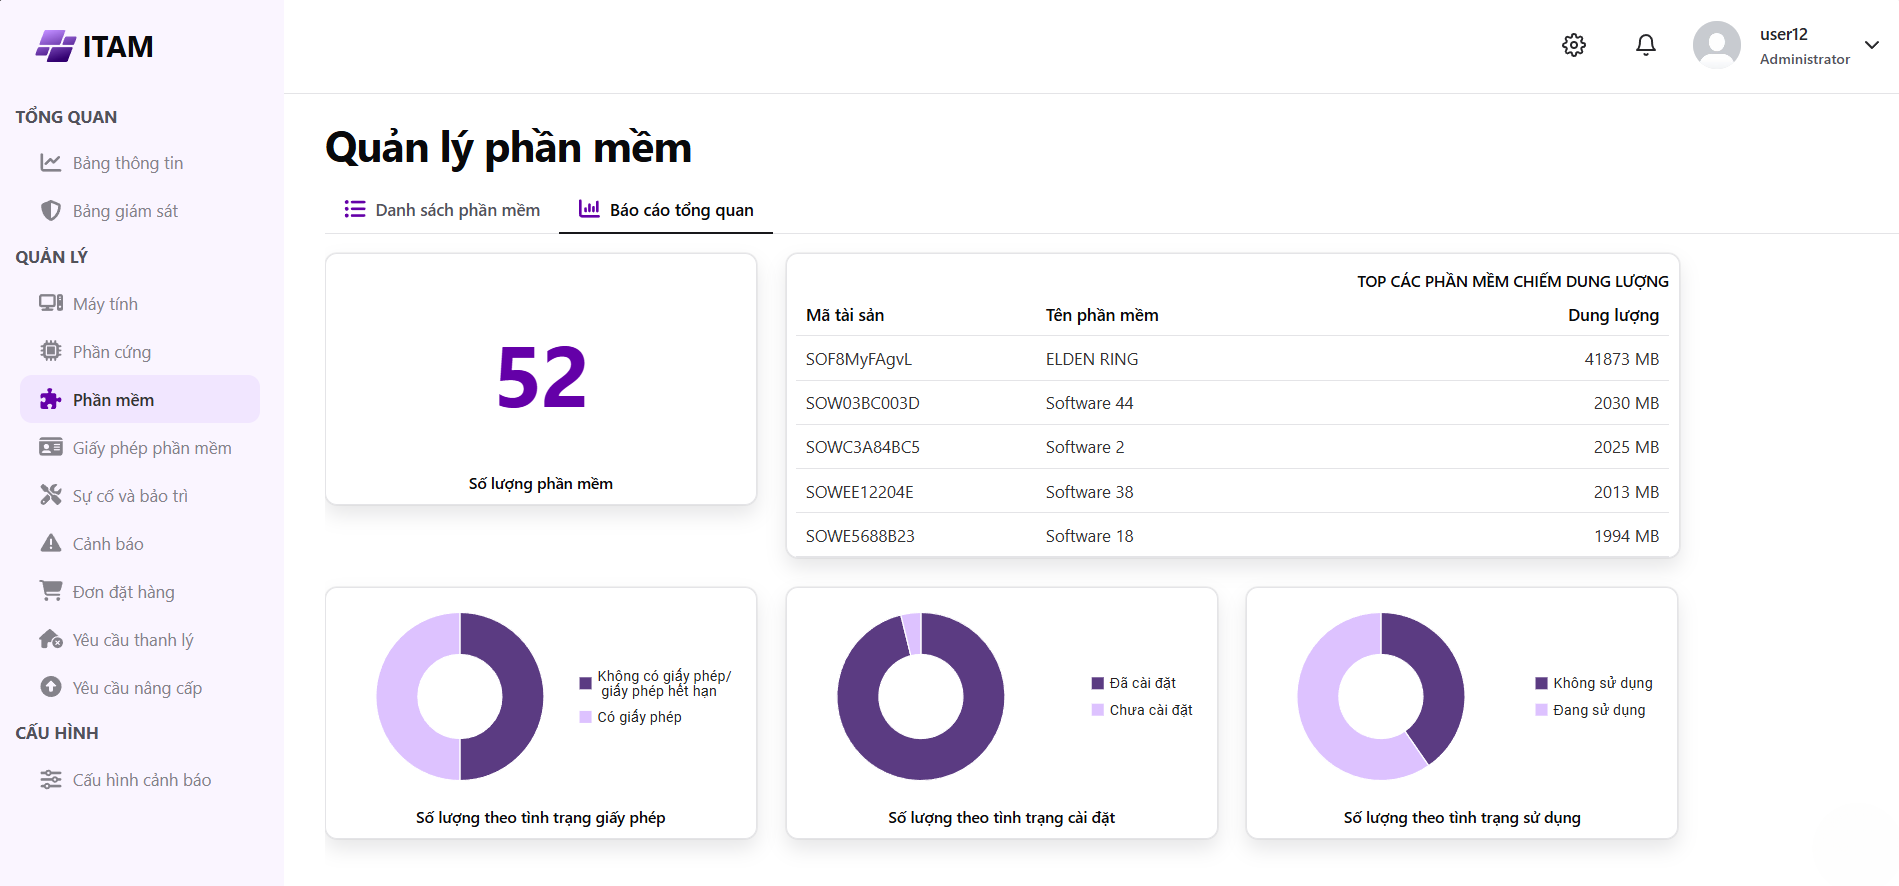
\includegraphics[width=14cm]{Images/C6/UI-Hienthuc/overview3.png}
        \vspace{15pt}
        \caption{Giao diện hiện thực tính năng Báo cáo tổng quan - phần mềm}
    \end{figure}
\end{itemize}

\section{Phụ lục Các bước cài đặt Collector}
\begin{itemize}[label=--]
    \item \textbf{Bước 1}\\
    Tải Collector từ Drive\\
    \begin{figure}[H]
        \centering
        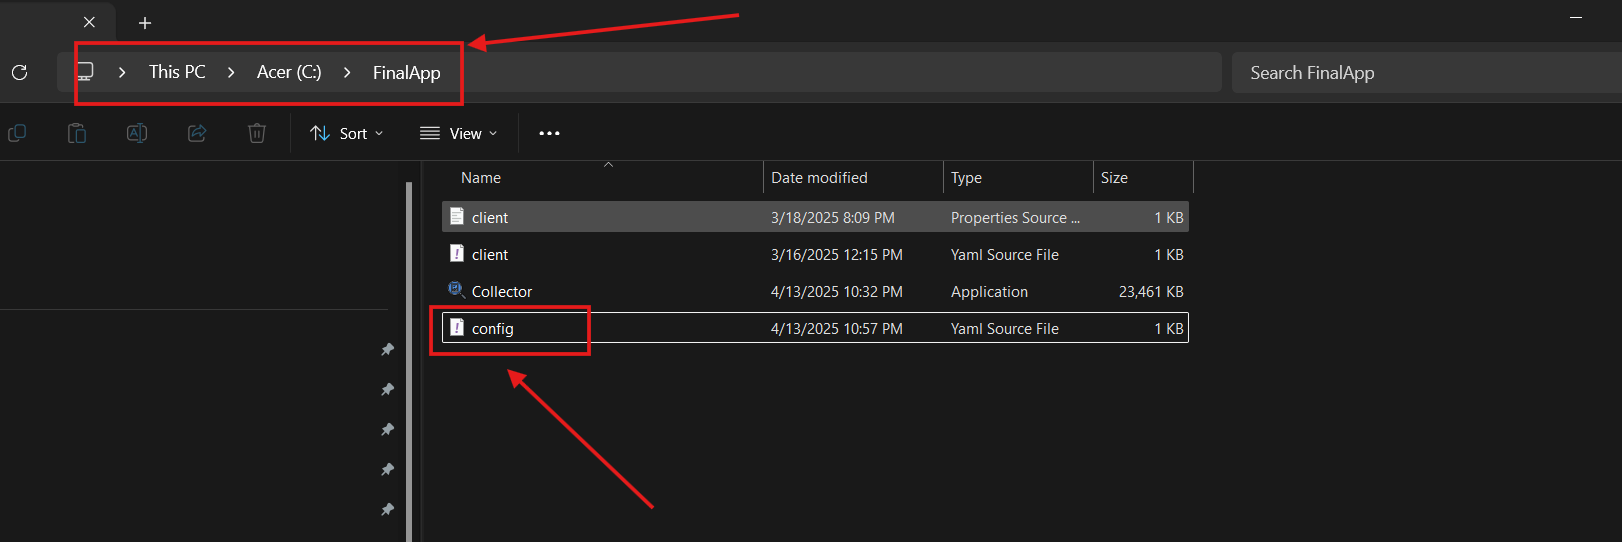
\includegraphics[width=14cm]{Images/C6/Cai-dat-Collector/collector1.png}
        \vspace{15pt}
        \caption{Thư mục chứa Collector}
    \end{figure}
    Đảm bảo đường dẫn thư mục như trong hình.\\
    Mở file Config bằng notepad\\
    \begin{figure}[H]
        \centering
        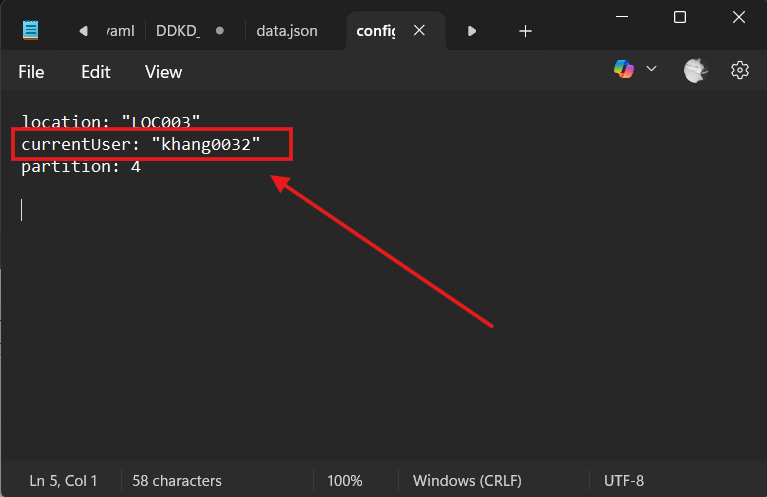
\includegraphics[width=14cm]{Images/C6/Cai-dat-Collector/collector2.png}
        \vspace{15pt}
        \caption{File Config cho Collector}
    \end{figure}
    Thay đổi dòng currentUser thành tên máy tính (ví dụ “khang0032” như trên hình) sau đó lưu lại

    \item \textbf{Bước 2}\\
    \begin{figure}[H]
        \centering
        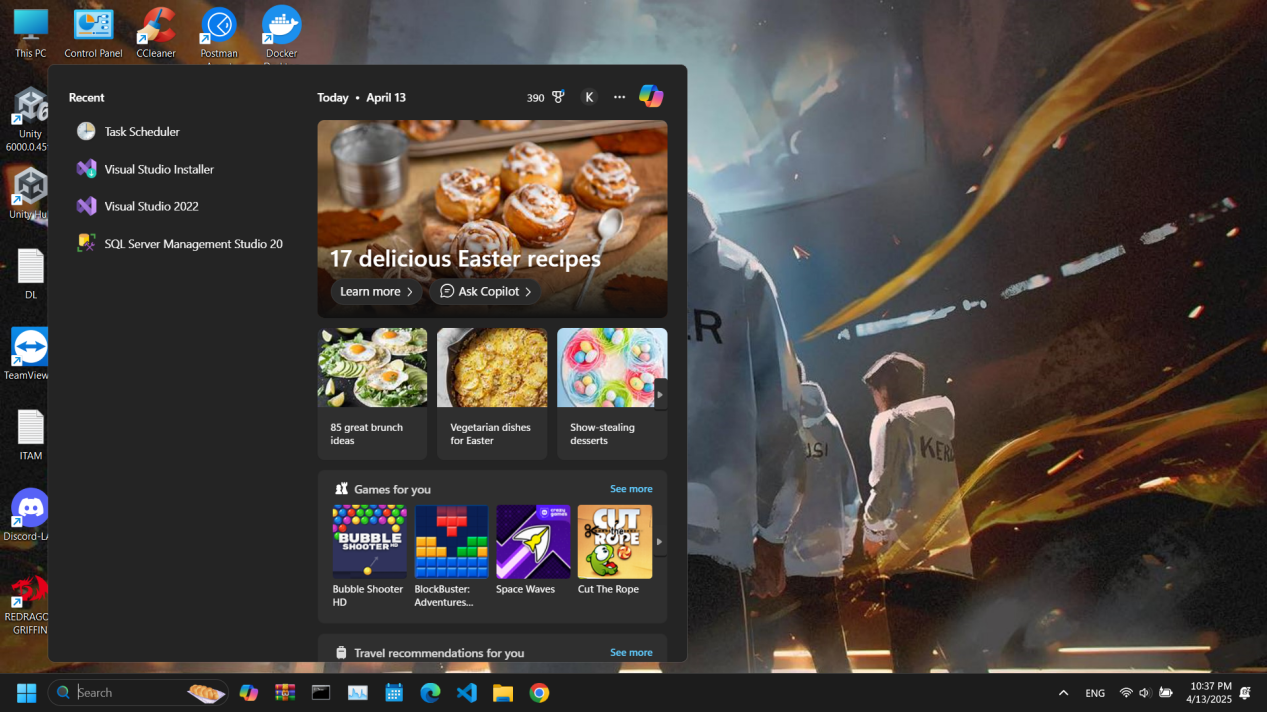
\includegraphics[width=14cm]{Images/C6/Cai-dat-Collector/collector3.png}
        \vspace{15pt}
        \caption{Tìm kiếm Task Scheduler}
    \end{figure}
    Tìm kiếm \textbf{Task Scheduler} trên thanh tìm kiếm\\
    Màn hình hiện ra như ở dưới
    \begin{figure}[H]
        \centering
        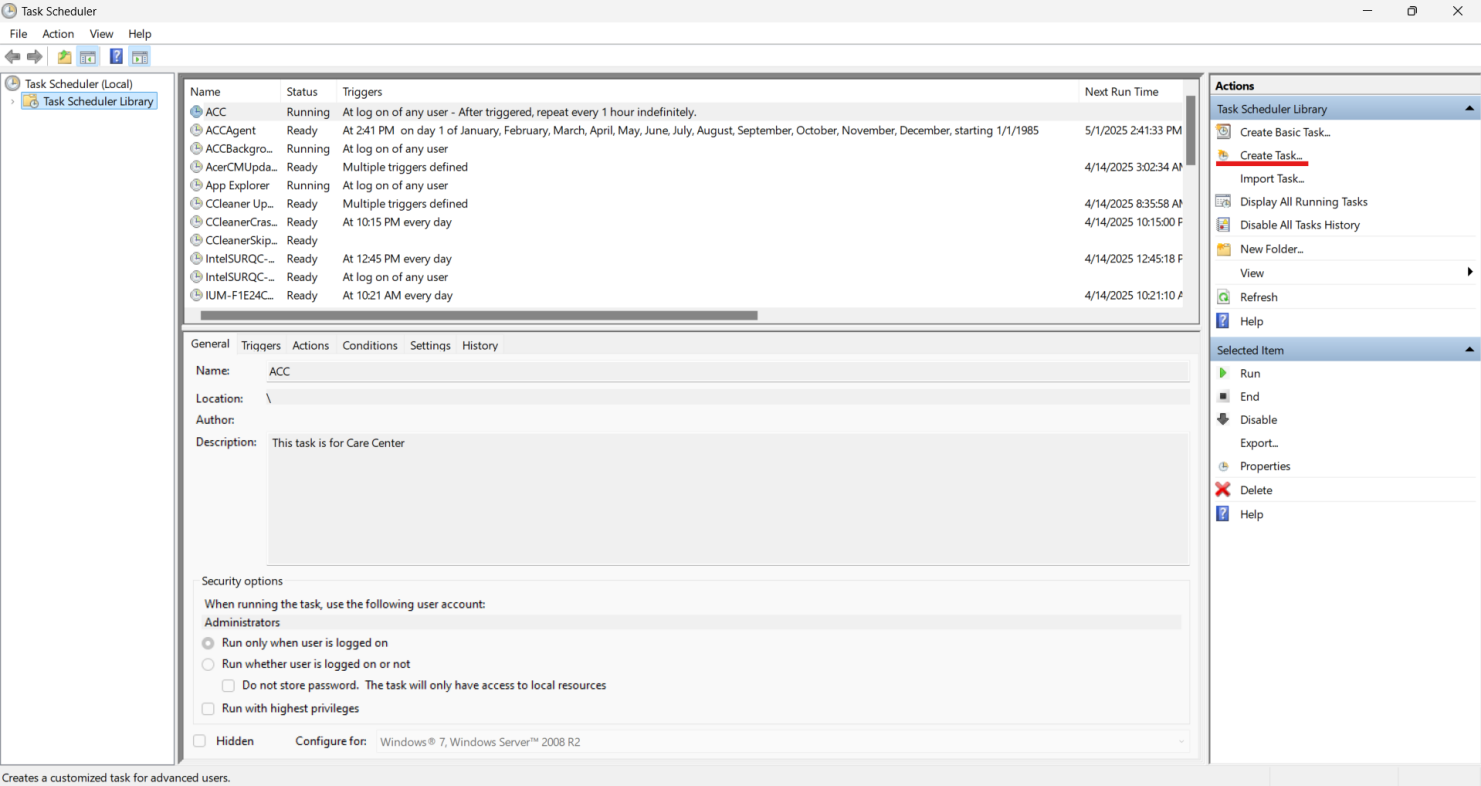
\includegraphics[width=14cm]{Images/C6/Cai-dat-Collector/collector4.png}
        \vspace{15pt}
        \caption{Giao diện Task Scheduler}
    \end{figure}
    Nhấn vào \textbf{Create Task} (như hình trên)\\
    \begin{figure}[H]
        \centering
        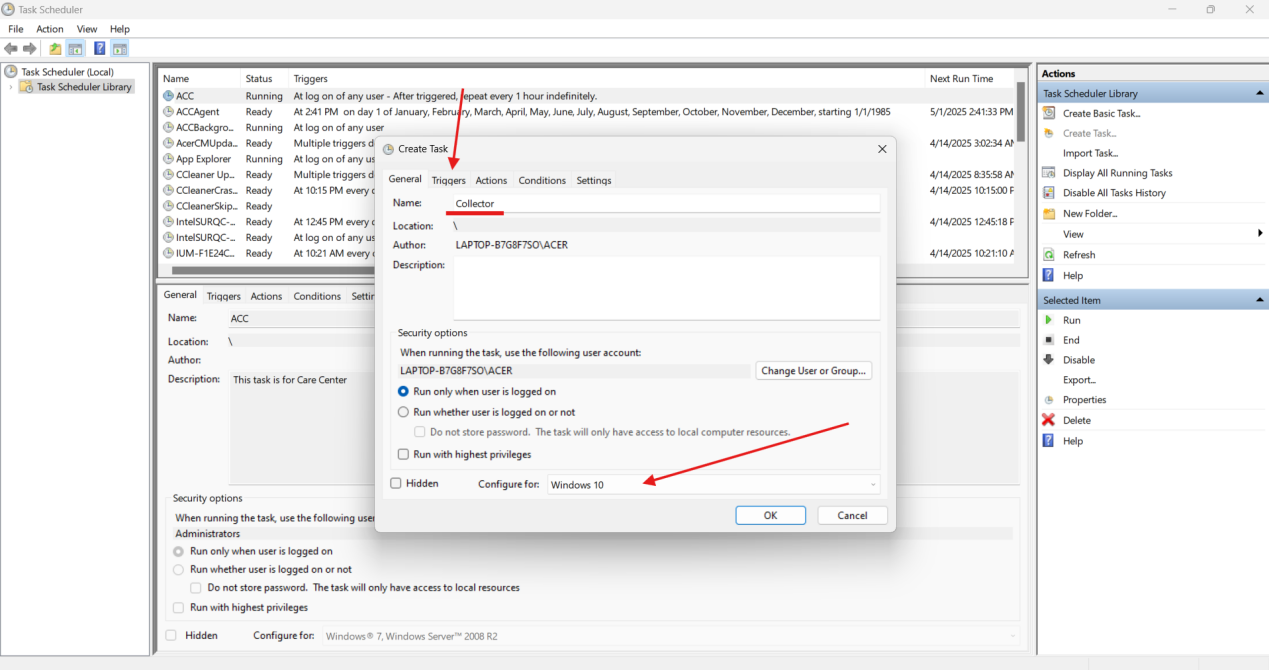
\includegraphics[width=14cm]{Images/C6/Cai-dat-Collector/collector5.png}
        \vspace{15pt}
        \caption{Giao diện Create Task}
    \end{figure}
    Cửa sổ hiện lên như hình trên. Sau đó, nhập tên vào ô \textbf{Name} , ở mục \textbf{Configure for} nhấn vào và chọn Windows 10. \\
    
    Sau khi đã điền tên và chọn hệ điều hành, nhấn chuyển qua Tab \textbf{Triggers} bên cạnh sẽ hiện màn hình như hình dưới.\\
    \begin{figure}[H]
        \centering
        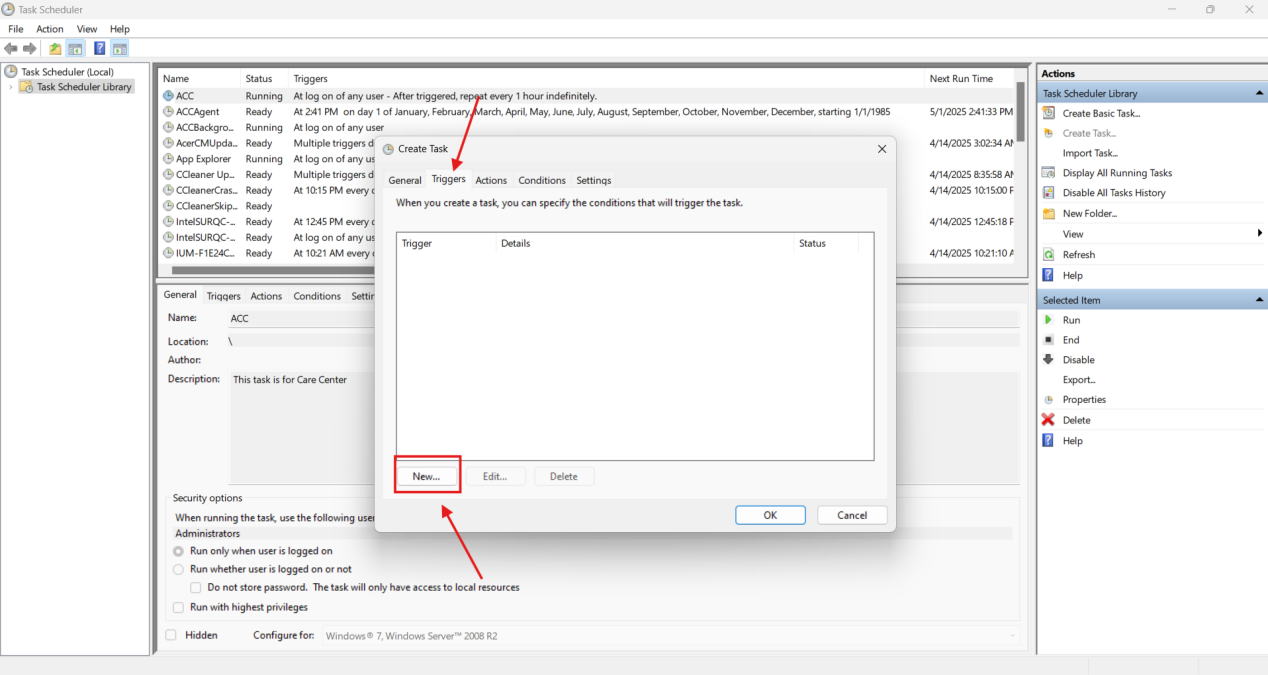
\includegraphics[width=14cm]{Images/C6/Cai-dat-Collector/collector6.png}
        \vspace{15pt}
        \caption{Giao diện Tab Trigger}     
    \end{figure}
    Tại màn hình này chọn New để tạo \textbf{Trigger} \\
    \begin{figure}[H]
        \centering
        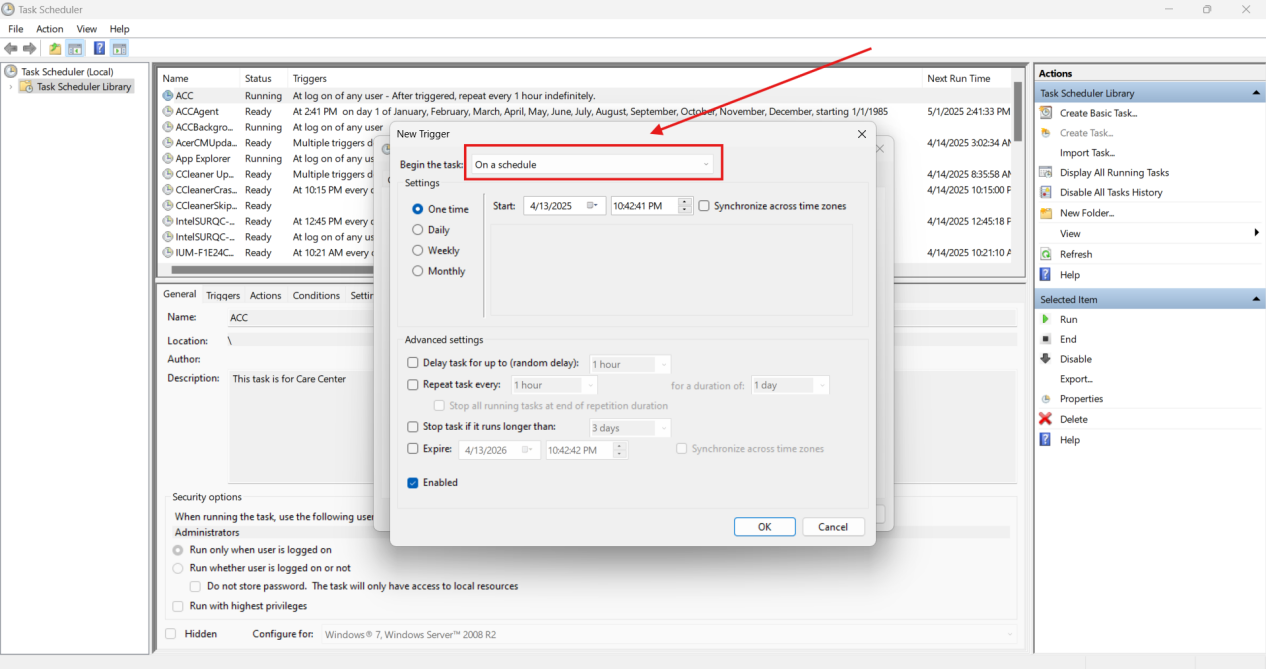
\includegraphics[width=14cm]{Images/C6/Cai-dat-Collector/collector7.png}
        \vspace{15pt}
        \caption{Giao diện Chọn Trigger}

    \end{figure}
    Click Vào ô \textbf{On a Schedule} như hình trên rồi chọn \textbf{At log on} như hình dưới, rồi nhấn \textbf{Ok} \\
    \begin{figure}[H]
        \centering
        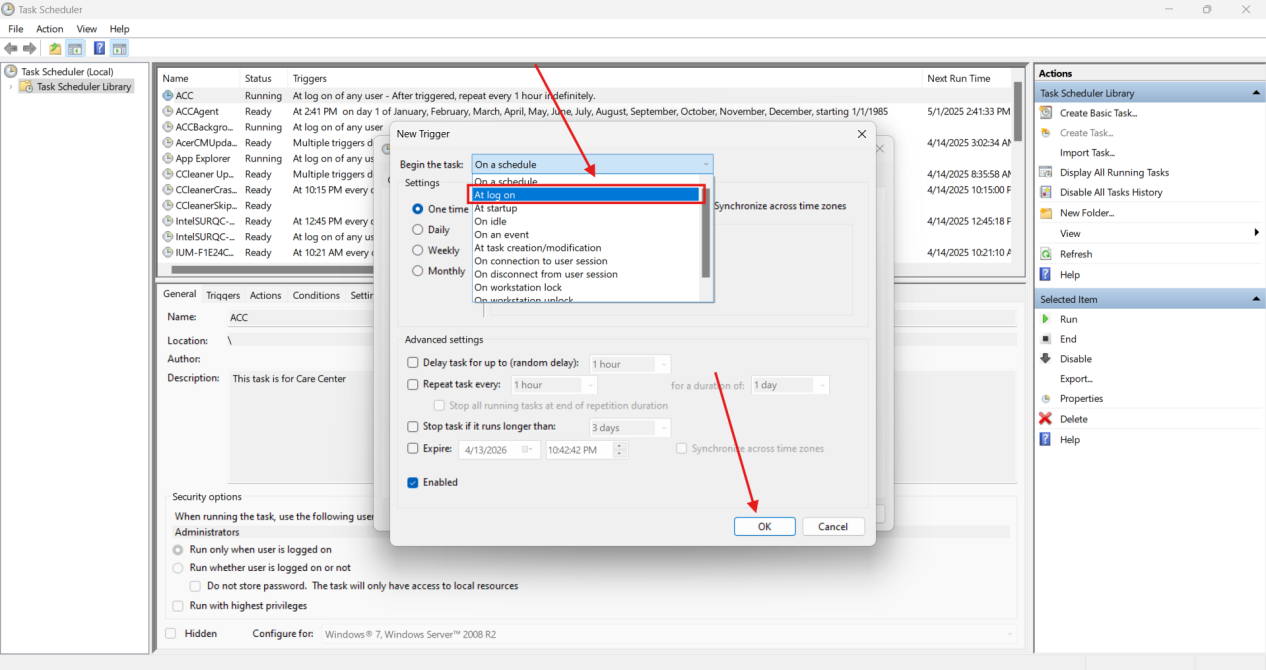
\includegraphics[width=14cm]{Images/C6/Cai-dat-Collector/collector8.png}
        \vspace{15pt}
        \caption{Chọn tùy chỉnh cho Trigger}
    \end{figure}

    \item \textbf{Bước 3}\\
    Sau khi đã tạo \textbf{trigger} xong, ấn chuyển qua tab Actions bên cạnh, màn hình hiện ra như ở dưới.\\
    \begin{figure}[H]
        \centering
        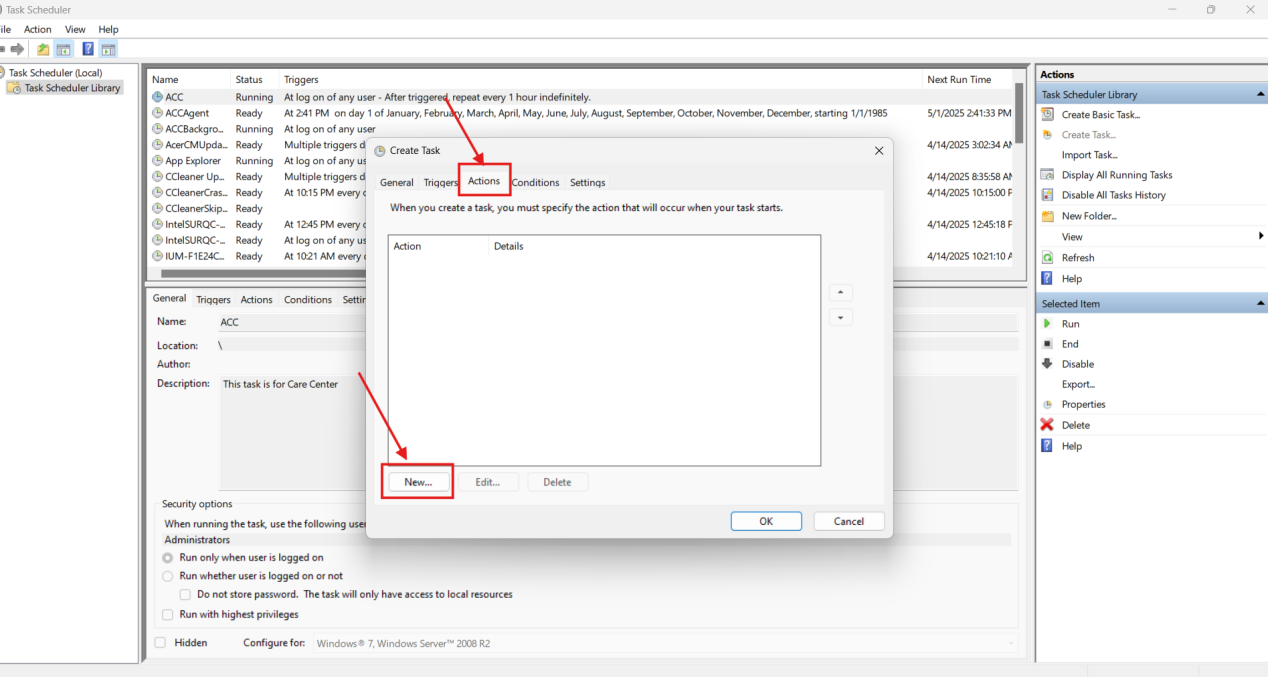
\includegraphics[width=14cm]{Images/C6/Cai-dat-Collector/collector9.png}
        \vspace{15pt}
        \caption{Giao diện Tab Action}
    \end{figure}
    Chọn \textbf{New} để tạo \textbf{Action} mới. \\

    Cửa sổ hiện lên (như hình dưới)\\
    \begin{figure}[H]
        \centering
        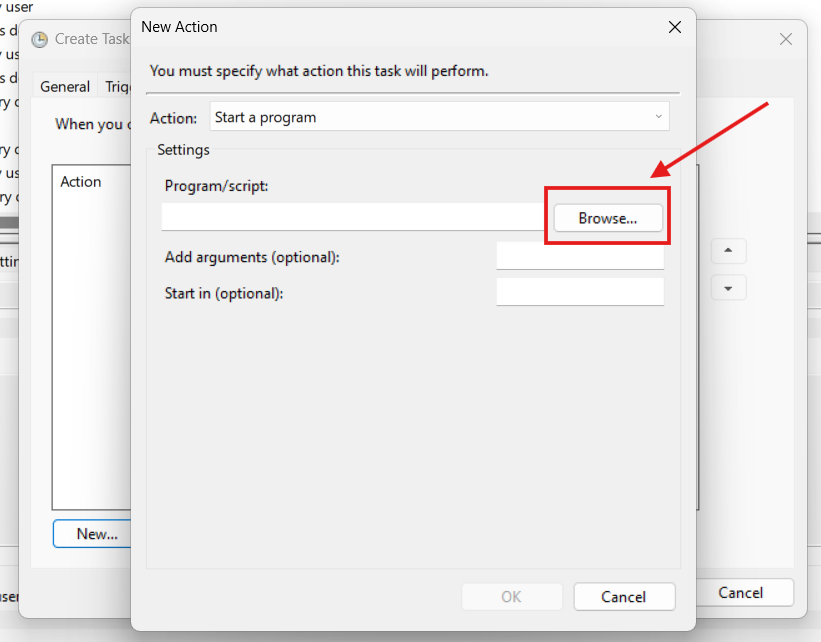
\includegraphics[width=0.8\linewidth]{Images/C6/Cai-dat-Collector/collector10.png}
        \vspace{15pt}
        \caption{Tùy chỉnh Action}
    \end{figure}
    Ấn chọn \textbf{Browse} để tìm kiếm \textbf{Collector.exe}\\
    \begin{figure}[H]
        \centering
        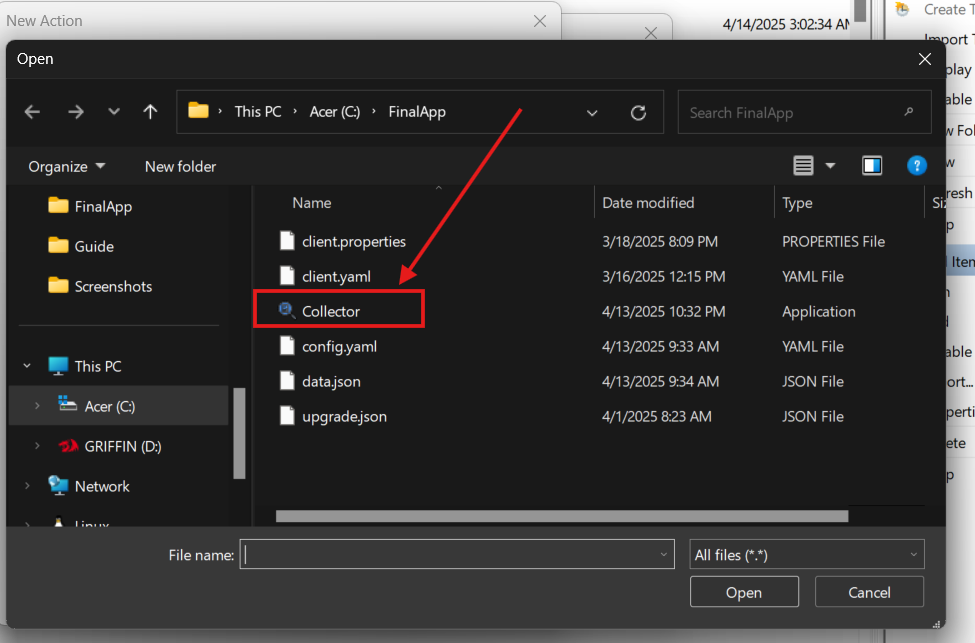
\includegraphics[width=0.7\linewidth]{Images/C6/Cai-dat-Collector/collector11.png}
        \vspace{15pt}
        \caption{Tìm kiếm Collector.exe}
    \end{figure}
    Sau khi chọn xong thì sẽ được màn hình như hình dưới. Sau đó nhấn \textbf{OK} để hoàn tất quá trình tạo Actions \\
    \begin{figure}[H]
        \centering
        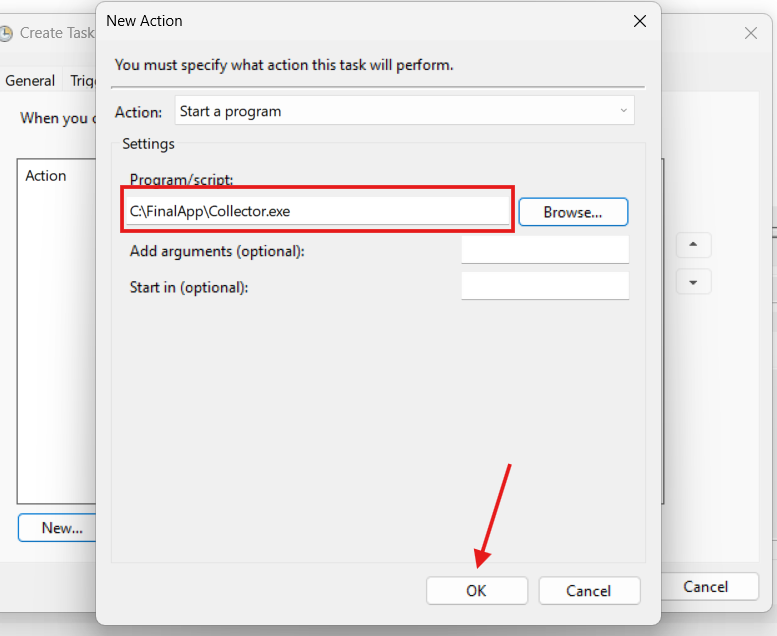
\includegraphics[width=0.7\linewidth]{Images/C6/Cai-dat-Collector/collector12.png}
        \vspace{15pt}
        \caption{Hoàn tất cài đặt Collector.exe}
    \end{figure}
    \textbf{Nhấn OK một lần nữa để hoàn tất quá trình cài đặt\\ 
Tool sẽ tự động khởi động và chạy ngầm khi khởi động lại máy.
}
\end{itemize}
\section{Phụ lục Hiện thực dự đoán nhu cầu nâng cấp RAM bằng Random Forest}
\begin{enumerate}
    \item \textbf{Mô tả dữ liệu}\\
    Dữ liệu được sử dụng lại từ phần LSTM tuy nhiên sẽ được xử lý lại để phù hợp với mục tiêu hiện thực. Dữ liệu sẽ được chia thành các chuỗi để đảm bảo khoảng cách giữa các hàng dữ liệu không quá 20 phút.
    \begin{itemize}[label=--]
        \item Thông tin người dùng
        \item Mức sử dụng RAM trung bình trong chuỗi dữ liệu
        \item Số lượng tiến trình trung bình trong chuỗi dữ liệu
        \item Mức sử dụng CPU trung bình trong một chuỗi dữ liệu
        \item Mức sử dụng RAM lớn nhất trong một chuỗi dữ liệu
        \item Mức sử dụng CPU lớn nhất trong một chuỗi dữ liệu
        \item Tổng dung lượng RAM mà máy tính có
        \item Độ dài của chuỗi, tổng thời gian của chuỗi
    \end{itemize}
     Sau khi đã trích xuất các cột dữ liệu cần, chúng ta tiến hành gán nhãn cho các máy tính. 
     \begin{itemize}[label=--]
        \item Nhãn 0: với máy không cần nâng cấp
        \item Nhãn 1: với các máy có RAM sẵn có là 16GB muốn nâng cấp thêm 8GB
        \item Nhãn 2: với các máy có RAM sẵn có là 8GB muốn nâng cấp thêm 8GB
        \item Nhãn 3: với các máy có RAM sẵn có từ 8 tới 16GB nhưng chỉ cần nâng cấp thêm 4GB
        \item Nhãn 4: với các máy có dung lượng RAM lớn hơn 16GB cần nâng cấp với lượng RAM lớn hơn 4GB.
     \end{itemize}
     \item \textbf{Huấn luyện dữ liệu với mô hình Random Forest}:\\
    Tham số:
    \begin{itemize}[label=--]
        \item n\_estimators: Số lượng cây trong rừng
        \item max\_depth: Giới hạn độ sâu tối đa của mỗi cây
        \item min\_samples\_leaf: Số mẫu tối thiểu trong một nút lá
    \end{itemize}
    \item \textbf{Đánh giá mô hình}:\\
    Bảng dưới đây thể hiện các chỉ số đánh giá hiệu suất của mô hình Random Forest trên tập kiểm tra, bao gồm Precision, Recall và F1-score cho từng nhãn (từ 0 đến 4), cùng với các chỉ số tổng hợp như Accuracy, Macro Average và Weighted Average. Đây là mô hình được sử dụng để dự đoán nhu cầu nâng cấp RAM của máy tính dựa trên dữ liệu hiệu suất hoạt động thu thập được trong quá trình sử dụng.
    \begin{longtable}{|p{0.1\textwidth}|p{0.12\textwidth}|p{0.2\textwidth}|p{0.2\textwidth}|}
    \caption{Đánh giá mô hình Random Forest}\\
    \hline
    \textbf{Nhãn}  & \textbf{Precision} & \textbf{Recall} & \textbf{F1-Score} \\
    \hline
    0 & 0.85 & 0.80 & 0.82 \\
    \hline
    1 & 0.92 & 0.95 & 0.93 \\
    \hline
    2 & 0.80 & 0.67 & 0.73 \\
    \hline
    3 & 0.75 & 0.60 & 0.67 \\
    \hline
    4 & 0.78 & 0.88 & 0.82 \\
    \hline
\end{longtable}
Kết quả đánh giá mô hình như sau:
 \begin{itemize}[label=--]
        \item Mô hình đạt Accuracy = 0.84, tức tỷ lệ dự đoán chính xác trên toàn bộ tập kiểm tra là 84%.
        \item Macro F1-score = 0.82 và Weighted F1-score = 0.84, thể hiện mô hình duy trì hiệu suất ổn định và tương đối cân bằng giữa các nhãn.
    \end{itemize}
Nhận xét:
\begin{itemize}[label=--]
        \item Nhãn 1 đạt F1-score = 0.93 với Precision = 0.92 và Recall = 0.95. Đây là lớp được mô hình dự đoán tốt nhất, có thể là do dữ liệu rõ ràng, số lượng mẫu đủ lớn và đặc trưng nhận diện dễ phân biệt.
        \item Nhãn 3 có F1-score = 0.67, thấp nhất trong các nhãn. Điều này cho thấy mô hình gặp khó khăn trong việc phân loại đúng các trường hợp yêu cầu nâng cấp thêm 4GB, khả năng do sự chồng chéo đặc trưng giữa các lớp hoặc thiếu dữ liệu đại diện.
        \item Các nhãn còn lại gồm 0, 2 và 4 có F1-score dao động từ 0.73 đến 0.82, thể hiện mức độ phân loại tốt và ổn định.
    \end{itemize}
=> Mô hình \textbf{Random Forest} đã thể hiện năng lực phân loại khá hiệu quả trong việc dự đoán nhu cầu nâng cấp RAM, đặc biệt trong các tình huống phổ biến như nâng từ 16GB lên 24GB (nhãn 1) hoặc không cần nâng cấp (nhãn 0). Với các chỉ số tổng hợp đạt mức cao, mô hình này có thể được tích hợp vào hệ thống quản lý tài sản CNTT như một thành phần hỗ trợ ra quyết định nâng cấp RAM một cách tự động, khách quan và có độ tin cậy cao.
\item Màn hình hiện thực dự đoán nhu cầu nâng cấp RAM:
\begin{figure}
    \centering
    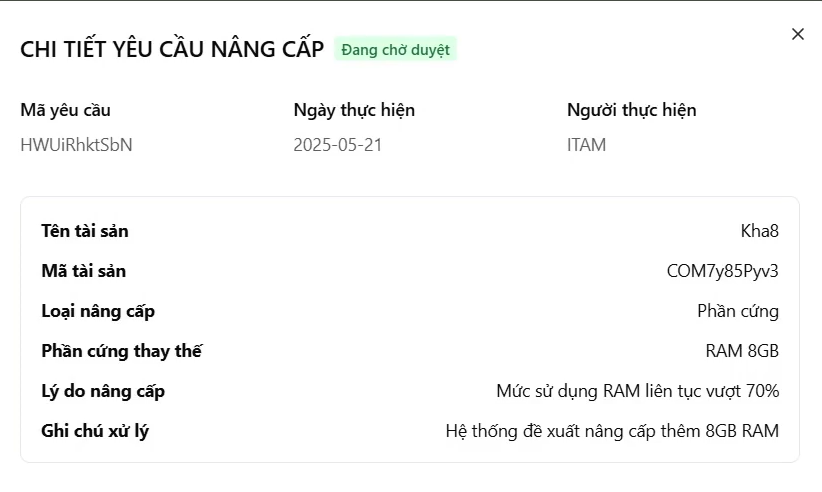
\includegraphics[width=0.5\linewidth]{Images/RamUpgrade.png}
    \caption{Đề xuất nâng cấp RAM}
    \label{fig:enter-label}
\end{figure}
\end{enumerate}
%   \begin{itemize}[label=\textbullet]

\section{Phụ lục Các kịch bản kiểm thử còn lại của hệ thống}
\begin{longtable}{
    |>{\raggedright\arraybackslash}p{0.05\textwidth}
    |>{\raggedright\arraybackslash}p{0.15\textwidth}
    |>{\raggedright\arraybackslash}p{0.2\textwidth}
    |>{\raggedright\arraybackslash}p{0.3\textwidth}
    |>{\raggedright\arraybackslash}p{0.2\textwidth}|
}
    \caption{Kịch bản kiểm thử module Quản lý người dùng} \\
    \hline
    \textbf{ID} & \textbf{Testcase} & \textbf{Description} & \textbf{Step} & \textbf{Kết quả} \\
    \hline
    \vspace{0.1pt} U01 & \vspace{0.1pt} Đăng nhập thành công & \vspace{0.1pt} Người dùng nhập đúng thông tin đăng nhập & 
    \begin{itemize}[leftmargin=*,topsep=0pt,itemsep=0pt,label=--]
        \item Open website
        \item Click on "Tài khoản"
        \item Enter "user7@example.com" into "Tài khoản"
        \item Enter "******" into "Mật khẩu"
        \item Click on "Đăng nhập"
        \item Redirect to Dashboard
    \end{itemize} &
    \begin{itemize}[leftmargin=*,topsep=0pt,itemsep=0pt,label=--]
        \item Hệ thống chuyển sang trang chủ, lưu accessToken và refreshToken vào localStorage
    \end{itemize} \\
    \hline    
    \vspace{0.1pt} U02 & \vspace{0.1pt} Đăng nhập thất bại & \vspace{0.1pt} Người dùng nhập sai tài khoản hay password & 
    \begin{itemize}[leftmargin=*,topsep=0pt,itemsep=0pt,label=--]
        \item Open website
        \item Click on "Tài khoản"
        \item Enter "user7" into "Tài khoản"
        \item Enter "******" into "Mật khẩu"
        \item Click on "Đăng nhập"
        \item Failed login attempt
    \end{itemize} &
    \begin{itemize}[leftmargin=*,topsep=0pt,itemsep=0pt,label=--]
        \item Hệ thống hiển thị thông báo lỗi "Vui lòng kiểm tra lại tài khoản hoặc mật khẩu". Không chuyển trang, không lưu token
    \end{itemize} \\
    \hline
    \vspace{0.1pt} U03 & \vspace{0.1pt} Chưa nhập thông tin đăng nhập & \vspace{0.1pt} Người dùng không nhập tài khoản hay password & 
    \begin{itemize}[leftmargin=*,topsep=0pt,itemsep=0pt,label=--]
        \item Open website
        \item Click on "Tài khoản"
        \item Enter "user7" into "Tài khoản"
        \item Click on "Đăng nhập"
    \end{itemize} &
    \begin{itemize}[leftmargin=*,topsep=0pt,itemsep=0pt,label=--]
        \item Hệ thống hiển thị thông báo lỗi "Bạn chưa nhập tài khoản đăng nhập" hoặc "Bạn chưa nhập mật khẩu". Không chuyển trang, không lưu token
    \end{itemize} \\
    \hline    
    \vspace{0.1pt} U04 & \vspace{0.1pt} Đăng xuất & \vspace{0.1pt} Người dùng đang đăng nhập chọn chức năng đăng xuất & 
    \begin{itemize}[leftmargin=*,topsep=0pt,itemsep=0pt,label=--]
        \item Open website
        \item Click on "Auser7ITStaff"
        \item Click on "Sign out"
    \end{itemize} &
    \begin{itemize}[leftmargin=*,topsep=0pt,itemsep=0pt,label=--]
        \item Hệ thống xóa accessToken và refreshToken khỏi localStorage, chuyển về trang đăng nhập
    \end{itemize} \\
    \hline    
    \vspace{0.1pt} U05 & \vspace{0.1pt} Xác thực đa yếu tố (MFA) & \vspace{0.1pt} Kiểm tra gửi mã OTP khi đăng nhập & &
    \begin{itemize}[leftmargin=*,topsep=0pt,itemsep=0pt,label=--]
        \item Chức năng chưa hoàn thiện
    \end{itemize} \\
    \hline
\end{longtable}
\begin{longtable}{
    |>{\raggedright\arraybackslash}p{0.05\textwidth}
    |>{\raggedright\arraybackslash}p{0.15\textwidth}
    |>{\raggedright\arraybackslash}p{0.2\textwidth}
    |>{\raggedright\arraybackslash}p{0.3\textwidth}
    |>{\raggedright\arraybackslash}p{0.2\textwidth}|
}
    \caption{Kịch bản kiểm thử module Quản lý vòng đời tài sản} \\
    \hline
    \textbf{ID} & \textbf{Testcase} & \textbf{Description} & \textbf{Step} & \textbf{Kết quả} \\
    \hline
    \vspace{0.1pt} L01 & \vspace{0.1pt} Tạo yêu cầu nâng cấp tài sản & \vspace{0.1pt} Tạo một yêu cầu nâng cấp cho một tài sản cụ thể & 
    \begin{itemize}[leftmargin=*,topsep=0pt,itemsep=0pt,label=--]
        \item Log into the website with an Administrator or ITStaff account
        \item Click on "Máy tính"
        \item Click on "COMiVT7eNQE"
        \item Click on "Gửi yêu cầu nâng cấp"
        \item Choose "CPU" for "Loại phần cứng cần nâng cấp"
        \item Enter "RAMBLVb7LVc" into "Phần cứng cần thay thế"
        \item Enter "RAMBLVb7LVc" into "Phần cứng cần thay thế"
        \item Enter "Thiết bị không đủ mạnh" into "Lý do nâng cấp"
        \item Click on "Gửi"
    \end{itemize} &
    \begin{itemize}[leftmargin=*,topsep=0pt,itemsep=0pt,label=--]
        \item Dữ liệu yêu cầu nâng cấp được tạo thành công. Khi Manager kiểm tra sẽ có yêu cầu nâng cấp vừa được tạo trong tình trạng "Đang chờ duyệt"
    \end{itemize} \\
    \hline
    \vspace{0.1pt} L02 & \vspace{0.1pt} Phê duyệt yêu cầu nâng cấp & \vspace{0.1pt} Phê duyệt yêu cầu nâng cấp tài sản bởi người quản lý & 
    \begin{itemize}[leftmargin=*,topsep=0pt,itemsep=0pt,label=--]
        \item Log into the website with a Manager account
        \item Click on "Yêu cầu nâng cấp"
        \item Click on "HWUUg49Igpa"
        \item Click on "Xác nhận phê duyệt yêu cầu"
        \item Click on "Đồng ý"
    \end{itemize} &
    \begin{itemize}[leftmargin=*,topsep=0pt,itemsep=0pt,label=--]
        \item Yêu cầu nâng cấp được phê duyệt thành công, trạng thái của yêu cầu nâng cấp sẽ là "Đã phê duyệt"
    \end{itemize} \\
    \hline
    \vspace{0.1pt} L03 & \vspace{0.1pt} Điền thông tin mua sắm tài sản & \vspace{0.1pt} Nhập thông tin mua sắm cho tài sản sau khi mua sắm tài sản & 
    \begin{itemize}[leftmargin=*,topsep=0pt,itemsep=0pt,label=--]
        \item Log into the website with a Manager account
        \item Click on "Máy tính"
        \item Click on "COMiVT7eNQE"
        \item Click on "Vòng đời tài sản"
        \item Enter 100000 for "Giá trị tài sản"
    \end{itemize} &
    \begin{itemize}[leftmargin=*,topsep=0pt,itemsep=0pt,label=--]
        \item Thông tin mua sắm tài sản được cập nhật với giá trị lúc mua sắm là 100000 VND
    \end{itemize} \\
    \hline
    \vspace{0.1pt} L04 & \vspace{0.1pt} Thay đổi thông tin triển khai tài sản & \vspace{0.1pt} Cập nhật thông tin triển khai khi đưa tài sản vào sử dụng sau khi đã mua sắm tài sản & 
    \begin{itemize}[leftmargin=*,topsep=0pt,itemsep=0pt,label=--]
        \item Log into the website with a Manager account
        \item Click on "Máy tính"
        \item Click on "COMiVT7eNQE"
        \item Click on "Vòng đời tài sản"
        \item Click on "Triển khai"
        \item Choose "Tầng 404, Tầng 4, Tòa nhà D, Hải Phòng" for "Vị trí"
    \end{itemize} &
    \begin{itemize}[leftmargin=*,topsep=0pt,itemsep=0pt,label=--]
        \item Thông tin triển khai tài sản được cập nhật thành công
    \end{itemize} \\
    \hline
    \vspace{0.1pt} L05 & \vspace{0.1pt} Gửi yêu cầu thanh lý tài sản & \vspace{0.1pt} Tạo yêu cầu thanh lý đối với một tài sản không còn sử dụng & 
    \begin{itemize}[leftmargin=*,topsep=0pt,itemsep=0pt,label=--]
        \item Log into the website with an Administrator or ITStaff account
        \item Click on "Máy tính"
        \item Click on "COMiVT7eNQE"
        \item Click on "Vòng đời tài sản"
        \item Click on "Thanh lý"
        \item Enter "Bán lại" for "Phương thức thanh lý"
        \item Enter "06/04/2025" for "Ngày thanh lý"
        \item Enter 80000 for "Giá bán cuối cùng"
        \item Enter "Disposal Company" for "Nhà cung cấp dịch vụ thanh lý"
        \item Enter "Đã cũ" for "Lý do thanh lý"
        \item Click on "Gửi yêu cầu thanh lý"
        \item Choose GPU and network to be sold with computer
        \item Click on "Gửi yêu cầu"
    \end{itemize} &
    \begin{itemize}[leftmargin=*,topsep=0pt,itemsep=0pt,label=--]
        \item Yêu cầu thanh lý tài sản được gửi thành công với trạng thái "Đang chờ duyệt"
    \end{itemize} \\
    \hline
    \vspace{0.1pt} L06 & \vspace{0.1pt} Phê duyệt yêu cầu thanh lý tài sản & \vspace{0.1pt} Quản lý xem xét và phê duyệt yêu cầu thanh lý & 
    \begin{itemize}[leftmargin=*,topsep=0pt,itemsep=0pt,label=--]
        \item Log into the website with a Manager account
        \item Click on "Yêu cầu thanh lý"
        \item Click on "DRQPpLtvJ0m"
        \item Click on "Duyệt"
        \item Click on "Đồng ý"
    \end{itemize} &
    \begin{itemize}[leftmargin=*,topsep=0pt,itemsep=0pt,label=--]
        \item Yêu cầu thanh lý được duyệt, trạng thái chuyển sang "Đã phê duyệt", hệ thống ghi nhận tài sản sẽ bị thanh lý
    \end{itemize} \\
    \hline
    \vspace{0.1pt} L07 & \vspace{0.1pt} Liên kết yêu cầu nâng cấp với tài sản & \vspace{0.1pt} Kiểm tra các yêu cầu nâng cấp của một tài sản cụ thể & 
    \begin{itemize}[leftmargin=*,topsep=0pt,itemsep=0pt,label=--]
        \item Log into the website with any account
        \item Click on "Máy tính"
        \item Click on "COMiVT7eNQE"
        \item Click on "Vòng đời tài sản"
        \item Click on "Sử dụng"
        \item Click on "Yêu cầu nâng cấp"
    \end{itemize} &
    \begin{itemize}[leftmargin=*,topsep=0pt,itemsep=0pt,label=--]
        \item Hệ thống hiển thị danh sách các yêu cầu nâng cấp đã được liên kết với tài sản
    \end{itemize} \\
    \hline
    \vspace{0.1pt} L08 & \vspace{0.1pt} Chỉnh sửa thông tin khấu hao tài sản & \vspace{0.1pt} Thay đổi các thông tin như giá trị còn lại, thời gian khấu hao, phương pháp khấu hao trong quá trình sử dụng tài sản để tính lại giá trị tài sản & 
    \begin{itemize}[leftmargin=*,topsep=0pt,itemsep=0pt,label=--]
        \item Log into the website with a Manager account
        \item Click on "Máy tính"
        \item Click on "COMiVT7eNQE"
        \item Click on "Vòng đời tài sản"
        \item Click on "Sử dụng"
        \item Click on "Khấu hao"
        \item Choose "SLS 5 Years" for "Phương pháp khấu hao"
        \item Enter "06/04/2025" for "Ngày bắt đầu có hiệu lực"
        \item Enter 100000 for "Tổng giá trị đã khấu hao"
        \item Enter 900000 for "Giá trị còn lại của tài sản"
    \end{itemize} &
    \begin{itemize}[leftmargin=*,topsep=0pt,itemsep=0pt,label=--]
        \item Thông tin khấu hao được cập nhật thành công
    \end{itemize} \\
    \hline
    \vspace{0.1pt} L09 & \vspace{0.1pt} Ghi nhận tài sản không thể nâng cấp & \vspace{0.1pt} Đánh dấu tài sản không phù hợp để nâng cấp và loại khỏi danh sách nâng cấp & 
    \begin{itemize}[leftmargin=*,topsep=0pt,itemsep=0pt,label=--]
        \item Log into the website with an Administrator or ITStaff account
        \item Click on "Yêu cầu nâng cấp"
        \item Click on the filter
        \item Click on "Lọc theo trạng thái"
        \item Click on "Đã từ chối"
    \end{itemize} &
    \begin{itemize}[leftmargin=*,topsep=0pt,itemsep=0pt,label=--]
        \item Tài sản được ghi nhận là không thể nâng cấp, trạng thái cập nhật trong hệ thống
    \end{itemize} \\
    \hline
    \vspace{0.1pt} L10 & \vspace{0.1pt} Xem lịch sử sự cố của tài sản & \vspace{0.1pt} Truy xuất và hiển thị các sự cố đã xảy ra với tài sản & 
    \begin{itemize}[leftmargin=*,topsep=0pt,itemsep=0pt,label=--]
        \item Log into the website with any account
        \item Click on "Máy tính"
        \item Click on "COMiVT7eNQE"
        \item Click on "Vòng đời tài sản"
        \item Click on "Sử dụng"
        \item Click on "Lịch sử sự cố"
    \end{itemize} &
    \begin{itemize}[leftmargin=*,topsep=0pt,itemsep=0pt,label=--]
        \item Hệ thống hiển thị danh sách các sự cố liên quan đến tài sản
    \end{itemize} \\
    \hline
    \vspace{0.1pt} L11 & \vspace{0.1pt} Xem lịch sử bảo trì của tài sản & \vspace{0.1pt} Truy xuất thông tin các lần bảo trì tài sản & 
    \begin{itemize}[leftmargin=*,topsep=0pt,itemsep=0pt,label=--]
        \item Log into the website with any account
        \item Click on "Máy tính"
        \item Click on "COMiVT7eNQE"
        \item Click on "Vòng đời tài sản"
        \item Click on "Sử dụng"
        \item Click on "Lịch sử bảo trì"
    \end{itemize} &
    \begin{itemize}[leftmargin=*,topsep=0pt,itemsep=0pt,label=--]
        \item Hệ thống hiển thị đầy đủ các thông tin bảo trì theo thời gian
    \end{itemize} \\
    \hline
    \vspace{0.1pt} L12 & \vspace{0.1pt} Xem lịch sử cảnh báo của tài sản & \vspace{0.1pt} Truy xuất các cảnh báo hệ thống đã ghi nhận đối với tài sản & 
    \begin{itemize}[leftmargin=*,topsep=0pt,itemsep=0pt,label=--]
        \item Log into the website with any account
        \item Click on "Máy tính"
        \item Click on "COMiVT7eNQE"
        \item Click on "Vòng đời tài sản"
        \item Click on "Sử dụng"
        \item Click on "Lịch sử cảnh báo"
    \end{itemize} &
    \begin{itemize}[leftmargin=*,topsep=0pt,itemsep=0pt,label=--]
        \item Hệ thống hiển thị danh sách cảnh báo của tài sản theo thứ tự thời gian
    \end{itemize} \\
    \hline
    \vspace{0.1pt} L13 & \vspace{0.1pt} Thay đổi trạng thái sử dụng của tài sản & \vspace{0.1pt} Cập nhật trạng thái tài sản: đang sử dụng, bảo trì, ngừng sử dụng & 
    \begin{itemize}[leftmargin=*,topsep=0pt,itemsep=0pt,label=--]
        \item Log into the website with any account
        \item Click on "Máy tính"
        \item Click on "COMiVT7eNQE"
        \item Click on status "Using"
        \item Choose "Maintenance"
    \end{itemize} &
    \begin{itemize}[leftmargin=*,topsep=0pt,itemsep=0pt,label=--]
        \item Trạng thái sử dụng của tài sản được cập nhật thành công trong hệ thống
    \end{itemize} \\
    \hline
    \vspace{0.1pt} L14 & \vspace{0.1pt} Gửi yêu cầu thanh lý phần cứng cụ thể & \vspace{0.1pt} Tạo yêu cầu thanh lý cho một bộ phận phần cứng cụ thể (RAM, ổ cứng,...) & 
    \begin{itemize}[leftmargin=*,topsep=0pt,itemsep=0pt,label=--]
        \item Log into the website with an Administrator or ITStaff account
        \item Click on "Phần cứng"
        \item Click on "RAMBLVb7LVc"
        \item Click on "Thanh lý"
        \item Enter "Bán lại" for "Phương thức thanh lý"
        \item Enter "06/04/2025" for "Ngày thanh lý"
        \item Enter 80000 for "Giá bán cuối cùng"
        \item Enter "Disposal Company" for "Nhà cung cấp dịch vụ thanh lý"
        \item Enter "Đã cũ" for "Lý do thanh lý"
        \item Click on "Gửi yêu cầu thanh lý"
        \item Click on "Gửi yêu cầu"
    \end{itemize} &
    \begin{itemize}[leftmargin=*,topsep=0pt,itemsep=0pt,label=--]
        \item Yêu cầu thanh lý phần cứng được gửi thành công, trạng thái ban đầu là "Đang chờ duyệt"
    \end{itemize} \\
    \hline
    \vspace{0.1pt} L15 & \vspace{0.1pt} Gửi yêu cầu thanh lý phần mềm cụ thể & \vspace{0.1pt} Gửi yêu cầu thanh lý đối với một phần mềm không còn sử dụng & 
    \begin{itemize}[leftmargin=*,topsep=0pt,itemsep=0pt,label=--]
        \item Log into the website with an Administrator or ITStaff account
        \item Click on "Phần mềm"
        \item Click on "SOFc1vLpaeW"
        \item Click on "Thanh lý"
        \item Enter "Bán lại" for "Phương thức thanh lý"
        \item Enter "06/04/2025" for "Ngày thanh lý"
        \item Enter 80000 for "Giá bán cuối cùng"
        \item Enter "Disposal Company" for "Nhà cung cấp dịch vụ thanh lý"
        \item Enter "Đã cũ" for "Lý do thanh lý"
        \item Click on "Gửi yêu cầu thanh lý"
        \item Click on "Gửi yêu cầu"
    \end{itemize} &
    \begin{itemize}[leftmargin=*,topsep=0pt,itemsep=0pt,label=--]
        \item Yêu cầu thanh lý phần mềm được tạo thành công với trạng thái ban đầu là "Đang chờ duyệt"
    \end{itemize} \\
    \hline
\end{longtable}